\documentclass[12pt,a4 paper]{extreport}
\usepackage[a4paper, top=1.0in, bottom=1.0in, left=1.0in, right=1.0in, heightrounded]{geometry}
\usepackage{ryan}
\usepackage[bottom]{footmisc}
\usepackage{pdfpages}

\pagestyle{fancy}
\fancyhf{}
\fancyhead[L]{\slshape\nouppercase{\leftmark}}
\fancyhead[R]{\thepage}
\renewcommand{\headrulewidth}{0.4pt}
\renewcommand{\arraystretch}{1.5}

\usepackage[
backend=biber,
style=alphabetic,
sorting=anyt
]{biblatex}
\addbibresource{biblio.bib}

\makeglossaries

\newacronym{h3math}{H3M}{H3 Mathematics}
\newacronym{h2fmath}{H2FM}{H2 Further Mathematics}
\newacronym{mat}{MAT}{Oxford Maths Admissions Test}
\newacronym{putnam}{PUTNAM}{William Lowell Putnam Mathematics Competition}

\begin{document}
%\includepdf{cover_page_uni}
% https://docs.google.com/document/d/1BnYV-5DkLfizphAaOHeH5S_hUeFZTAGS0Cg6YEeL7oA/edit?usp=sharing

\begin{titlepage}
\title{\sffamily\bfseries Fons}
\author{Ryan Joo Rui An}
\date{\today}

\vfill
\titlepic{
\includegraphics[width=0.5\textwidth]{images/logo.png}}
%\url{ryanjoo18.github.io/publications/fons.html}
\vfill
\vfill
\end{titlepage}

\maketitle
\pagebreak

\

\vfill

\begin{quote}
\textit{The mathematician does not study mathematics because it is useful; he studies it because he delights in it and he delights in it because it is beautiful.}

\begin{flushright}--- Henri Poincar\'{e} (1854--1912)\\
French mathematician and theoretical physicist\end{flushright}
\end{quote}

\vfill

\copyright 2024 Ryan Joo Rui An.\\
Text licensed under \href{https://creativecommons.org/licenses/by-sa/4.0/}{CC-by-SA-4.0}. Source files licensed under \href{https://www.mit.edu/~amini/LICENSE.md}{MIT License}.

This is (still!) an incomplete draft. Please send corrections and comments to \url{ryanjooruian18@gmail.com}, or pull-request at \url{https://github.com/Ryanjoo18/fons}.

Last updated \today.
\thispagestyle{empty}

\chapter*{Preface}
\emph{Fons}, derived from the Latin word for source or fountain, introduces the core concepts of university-level mathematics. Just as a fountain provides a continuous wellspring of water, \emph{Fons} aims to be a continuous source of knowledge for you.

At this moment of writing, I am a high school student working on my A Level studies in Singapore. I have about 11 years of participating in mathematics competitions, including three years of experience in mental arithmetic and the rest few years in mathematics olympiad.

This book mainly serves as my notes when studying mathematics at the university level. Feel free to refer to it too.

\

\begin{flushright}
Ryan Joo Rui An\\
\today\\
Singapore, SG
\end{flushright}
\pagebreak

\chapter*{Introduction}
The book is divided into the following sections:
\begin{enumerate}
\item \textbf{preliminary topics} such as basic set theory, 
\item \textbf{abstract algebra} which follows \cite{dummit-foote}, 
\item \textbf{linear algebra} which follows \cite{hoffman-kunze}, 
\item \textbf{real analysis} which follows \cite{rudin,apostol}, and
\item \textbf{complex analysis} which follows \cite{ahlfors}.
\end{enumerate}

The chapters in this book are structured as follows:
\begin{itemize}
\item A \textbf{theoretical portion}, which starts off with a couple of definitions coupled with examples, followed by theorems and propositions built upon the definitions.
\item A series of \textbf{exercises}.
\item Full \textbf{solutions} to the exercises.
\end{itemize}

The reader is not assumed to have any mathematical prerequisites, althrough some experience with proofs may be helpful.

\section*{Problem Solving}
In \cite{polya}, George P\'{o}lya outlined the following problem solving cycle:
\begin{enumerate}
\item \textbf{Understand the problem}

Ask yourself the following questions:
\begin{itemize}
\item Do you understand all the words used in stating the problem?
\item Is it possible to satisfy the condition? Is the condition sufficient to determine the unknown? Or is it insufficient? Or redundant? Or contradictory?
\item What are you asked to find or show? Can you restate the problem in your own words?
\item Draw a figure. Introduce suitable notation.
\item Is there enough information to enable you to find a solution?
\end{itemize}

\item \textbf{Devise a plan}

A partial list of heuristics -- good rules of thumb to solve problems -- is included:
\begin{multicols}{2}
\begin{itemize}
\item Guess and check
\item Look for a pattern
\item Make an orderly list
\item Draw a picture
\item Eliminate possibilities
\item Solve a simpler problem
\item Use symmetry
\item Use a model
\item Consider special cases
\item Work backwards
\item Use direct reasoning
\item Use a formula
\item Solve an equation
\item Be ingenious
\end{itemize}
\end{multicols}

\item \textbf{Execute the plan}

This step is usually easier than devising the plan. In general, all you need is care and patience, given that you have the necessary skills. Persist with the plan that you have chosen. If it continues not to work discard it and choose another. Don't be misled, this is how mathematics is done, even by professionals.

\begin{itemize}
\item Carrying out your plan of the solution, check each step. Can you see clearly that the step is correct? Can you prove that it is correct?
\end{itemize}

\item \textbf{Check and expand}

P\'{o}lya mentions that much can be gained by taking the time to reflect and look back at what you have done, what worked, and what didn't. Doing this will enable you to predict what strategy to use to solve future problems.

Look back reviewing and checking your results. Ask yourself the following questions:
\begin{itemize}
\item Can you check the result? Can you check the argument?
\item Can you derive the solution differently? Can you see it at a glance?
\item Can you use the result, or the method, for some other problem?
\end{itemize}
\end{enumerate}

Building on P\'{o}lya's problem solving strategy, Schoenfeld \cite{schoenfeld} came up with the following framework for problem solving, consisting of four components:
\begin{enumerate}
\item \textbf{Cognitive resources}: the body of facts and procedures at one's disposal.
\item \textbf{Heuristics}: `rules of thumb' for making progress in difficult situations.
\item \textbf{Control}: having to do with the efficiency with which individuals utilise the knowledge at their disposal. Sometimes, this is referred to as metacognition, which can be roughly translated as `thinking about one's own thinking'.
\begin{enumerate}
\item These are questions to ask oneself to monitor one's thinking.
\begin{itemize}
    \item What (exactly) am I doing? [Describe it precisely.] Be clear what I am doing NOW. Why am I doing it? [Tell how it fits into the solution.]
    \item Be clear what I am doing in the context of the BIG picture -- the solution. Be clear what I am going to do NEXT.
\end{itemize}

\item Stop and reassess your options when you
\begin{itemize}
    \item cannot answer the questions satisfactorily [probably you are on the wrong track]; OR
    \item are stuck in what you are doing [the track may not be right or it is right but it is at that moment too difficult for you].
\end{itemize}

\item Decide if you want to
\begin{itemize}
    \item carry on with the plan,
    \item abandon the plan, OR
    \item put on hold and try another plan.
\end{itemize}
\end{enumerate}

\item \textbf{Belief system}: one's perspectives regarding the nature of a discipline and how one goes about working on it.
\end{enumerate}
\pagebreak

\tableofcontents

\printglossary[type=\acronymtype]

% Materials to be cleared:
% https://www.seab.gov.sg/docs/default-source/national-examinations/syllabus/alevel/2022syllabus/9649_y22_sy.pdf
% https://www.cambridgeinternational.org/Images/597381-2023-2025-syllabus.pdf

\part{Preliminaries}
\chapter{Mathematical Reasoning and Logic}
% https://www.maths.ox.ac.uk/system/files/attachments/study_public_0.pdf

\section{Logical statements and notation}
It is useful to be familiar with the following terminology.
\begin{itemize}
\item A \vocab{definition} is a precise and unambiguous description of the meaning of a mathematical term. It characterises the meaning of a word by giving all the properties and only those properties that must be true.
\item A \vocab{theorem} is a true mathematical statement that can be proven mathematically. In a mathematical paper, the term theorem is often reserved for the most important results.
\item A \vocab{lemma} is a minor result whose sole purpose is to help in proving a theorem. It is a stepping stone on the path to proving a theorem. Very occasionally lemmas can take on a life of their own.
\item A \vocab{corollary} is a result in which the (usually short) proof relies heavily on a given theorem. We often say that ``this is a corollary of Theorem A''.
\item A \vocab{proposition} is a proven and often interesting result, but generally less important than a theorem.
\item A \vocab{conjecture} is a statement that is unproved, but is believed to be true.
\item An \vocab{axiom} is a statement that is assumed to be true without proof. These are the basic building blocks from which all theorems are proven.
\item An \vocab{identity} is a mathematical expression giving the equality of two (often variable) quantities.
\item A \vocab{paradox} is a statement that can be shown, using a given set of axioms and definitions, to be both true and false. Paradoxes are often used to show the inconsistencies in a flawed theory.
\end{itemize}

\subsection{Notation}
A \vocab{proposition} is a sentence which has exactly one truth value, i.e. it is either true or false, but not both and not neither. A proposition is denoted by uppercase letters such as $P$ and $Q$. If the proposition $P$ depends on a variable $x$, it is sometimes helpful to denote it by $P(x)$. 

We can so some algebra on propositions, which include
\begin{enumerate}[label=(\roman*)]
\item \vocab{equivalence}, denoted by $P \equiv Q$, which means $P$ and $Q$ are logically equivalent statements;

\item \vocab{conjunction}, denoted by $P \land Q$, which means ``$P$ and $Q$'';

\item \vocab{disjunction}, denoted by $P \lor Q$, which means ``$P$ or $Q$'';

\item \vocab{negation}, denoted by $\lnot P$, which means ``not $P$''.
\end{enumerate}

Here are some useful properties when handling logical statements. You can easily prove all of them using truth tables.
\begin{itemize}
\item Double negation law:
\[ P \equiv \lnot(\lnot P) \]

\item Commutative property:
\[ P \land Q \equiv Q \land P, \quad P \lor Q \equiv Q \lor P \]

\item Associative property for conjunction: 
\[ (P\land Q)\land R \equiv P\land (Q\land R) \]

\item Associative property for disjunction: 
\[ (P\lor Q)\lor R \equiv P\lor (Q\lor R) \]

\item Distributive property for conjunction across disjunction: 
\[ P\land(Q\lor R) \equiv (P\land Q)\lor(P\land Q) \]

\item Distributive property for disjunction across conjunction: 
\[ P\lor(Q\land R) \equiv (P\lor Q)\land(P\lor R) \]

\item \textbf{De Morgan's Laws}:
\[ \lnot(P \lor Q) \equiv (\lnot P \land \lnot Q) \]
\[ \lnot (P\land Q) \equiv (\lnot P\lor \lnot Q) \]
\end{itemize}

\begin{exercise}{}{}
Assume that $x$ is a fixed real number. What is the negation of the statement $1<x<2$?
\end{exercise}
\begin{solution}
The negation of $1<x<2$ is ``it is not the case that $1<x<2$”. However this is not useful.

Note that $1<x<2$ means $1<x$ and $x<2$. Let $P:1<x$ and $Q:x<2$. Then the statement $1<x<2$ is $P \land Q$.

By De Morgan's Laws, we have $\lnot (P \land Q) \equiv \lnot P \lor \lnot Q$.

The \emph{Trichotomy Axiom of real numbers} states that given fixed real numbers $a$ and $b$, exactly one of the statements $a<b, a=b, b<a$ is true. Hence $\lnot P \equiv \lnot (1<x) \equiv (x \le 1)$ and $\lnot Q \equiv \lnot (x<2) \equiv (x \ge 2)$.

Thus
\[ \lnot (1<x<2) \equiv \lnot (P \land Q) \equiv \lnot P \lor \lnot Q \equiv (1 \ge x) \lor (x \ge 2). \]

Therefore the negation of $1<x<2$ is logically equivalent to the statement $x \le 1$ or $x \ge 2$.
\end{solution}

\begin{exercise}{}{}
Assume that $n$ is a fixed positive integer. Find a useful denial of the statement
\[ n = 2 \text{ or } n \text{ is odd.} \]
\end{exercise}
\begin{solution}
Using De Morgan's Laws,
\begin{align*}
\lnot [(n = 2) \lor (n \text{ is odd})] &\equiv \lnot(n = 2) \land \lnot(n \text{ is odd}) \\
&\equiv (n \neq 2) \land (n \text{ is even})
\end{align*}
where we are using the fact that every integer is either even or odd, but not both.

Thus a useful denial of the given statement is: $n$ is an even integer other than 2.
\end{solution}
\pagebreak

\subsection{If, only if, $\implies$}
\vocab{Implication} is denoted by $P \implies Q$, which means ``$P$ implies $Q$'', i.e. if $P$ holds then $Q$ also holds. It is equivalent to saying ``If $P$ then $Q$''. The only case when $P \implies Q$ is false is when the hypothesis $P$ is true and the conclusion $Q$ is false.

$P \implies Q$ is known as a \vocab{conditional statement}. $P$ is known as the \vocab{hypothesis}, $Q$ is known as the \vocab{conclusion}.

Statements of this form are probably the most common, although they may sometimes appear quite differently. The following all mean the same thing:
\begin{enumerate}[label=(\roman*)]
\item if $P$ then $Q$;
\item $P$ implies $Q$;
\item $P$ only if $Q$;
\item $P$ is a sufficient condition for $Q$;
\item $Q$ is a necessary condition for $P$.
\end{enumerate}

The \vocab{converse} of $P \implies Q$ is given by $Q \implies P$; both are not logically equivalent.

The \vocab{inverse} of $P \implies Q$ is given by $\lnot P \implies \lnot Q$, i.e. the hypothesis and conclusion of the statement are both negated.

The \vocab{contrapositive} of $P \implies Q$ is given by $\lnot Q \implies \lnot P$; both are logically equivalent.

\textbf{How to prove:} To prove $P \implies Q$, start by assuming that $P$ holds and try to deduce through some logical steps that $Q$ holds too. Alternatively, start by assuming that $Q$ does not hold and show that $P$ does not hold (that is, we prove the contrapositive).
\pagebreak

\subsection{If and only if, iff, $\iff$}
\vocab{Bidirectional implication} is denoted by $P \iff Q$, which means both $P \implies Q$ and $Q \implies P$. We can read this as ``$P$ if and only if $Q$''. The letters ``iff'' are also commonly used to stand for ‘if and only if’.
\[ P \iff Q \equiv (P \implies Q) \land (Q \implies P) \]

$P \iff Q$ is true exactly when $P$ and $Q$ have the same truth value.

$P \iff Q$ is known as a \vocab{biconditional statement}.

These statements are usually best thought of separately as ‘if’ and ‘only if’ statements.

\textbf{How to prove:} To prove $P \iff Q$, prove the statement in both directions, i.e. prove both $P \implies Q$ and $Q \implies P$. Remember to make very clear, both to yourself and in your written proof, which direction you are doing.
\pagebreak

\subsection{Quantifiers}
The \vocab{universal quantifier} is denoted by $\forall$, which means ``for all'' or ``for every''. An universal statement has the form $\forall x\in X, P(x)$.

The \vocab{existential quantifier} is denoted by $\exists$, which means ``there exists''. An existential statement has the form $\exists x\in X, P(x)$, where $X$ is known as the \vocab{domain}.

These are versions of De Morgan's laws for quantifiers:
\[ \lnot \forall x\in X,P(x) \equiv \exists x\in X,\lnot P(x) \]
\[ \lnot \exists x\in X,P(x) \equiv \forall x\in X,\lnot P(x) \]

\begin{exercise}{}{}
Find a useful denial of the statement
\[ \text{for all real numbers } x, \text{ if } x>2, \text{ then } x^2>4 \]
\end{exercise}
\begin{solution}
In logical notation, this statement is $(\forall x \in \RR)[x>2 \implies x^2>4]$.
\begin{align*}
\lnot\{(\forall x \in \RR)[x>2 \implies x^2>4]\} 
&\equiv (\exists x \in \RR) \lnot[x>2 \implies x^2>4] \\
&\equiv (\exists x \in \RR) \lnot [(x\le2) \lor (x^2>4)] \\
&\equiv (\exists x \in \RR) [(x>2) \land (x^2\le4)]
\end{align*}
Therefore a useful denial of the statement is:
\[ \text{there exists a real number } x \text{ such that } x>2 \text{ and } x^2\le4. \] 
\end{solution}

\begin{exercise}{}{}
Negate surjectivity.
\end{exercise}
\begin{solution}
If $f:X\to Y$ is not surjective, then it means that there exists $y \in Y$ not in the image of $X$, i.e. for all $x$ in $X$ we have $f(x)\neq y$.
\begin{align*}
\lnot \forall y \in Y, \exists x \in X, f(x)=y 
&\iff \exists y \in Y, \lnot (\exists x \in X, f(x)=y) \\
&\iff \exists y \in Y, \forall x \in X, \lnot (f(x)=y) \\
&\iff \exists y \in Y, \forall x \in X, f(x) \neq y
\end{align*}
\end{solution}

\textbf{How to prove:} To prove a statement of the form $\forall x \in X \suchthat P(x)$’, start the proof with ‘Let $x \in X$.’ or ‘Suppose $x \in X$ is given.’ to address the quantifier with an arbitrary $x$; provided no other assumptions about $x$ are made during the course of proving $P(x)$, this will prove the statement for all $x \in X$. 

\textbf{How to prove:} To prove a statement of the form $\exists x \in X \suchthat P(x)$, there is not such a clear steer about how to continue: you may need to show the existence of an $x$ with the right properties; you may need to demonstrate logically that such an $x$ must exist because of some earlier assumption, or it may be that you can show constructively how to find one; or you may be able to prove by contradiction, supposing that there is no such $x$ and consequently arriving at some inconsistency.

\begin{remark}
Read from left to right, and as new elements or statements are introduced they are allowed to depend on previously introduced elements but cannot depend on things that are yet to be mentioned.
\end{remark}

\begin{remark}
To avoid confusion, it is a good idea to keep to the convention that the quantifiers come first, before any statement to which they relate.
\end{remark}
\pagebreak

\section{Proofs}
\subsection{Direct proof}
A direct proof of $P \implies Q$ is a series of valid arguments that start with the hypothesis $P$ and end with the conclusion $Q$. It may be that we can start from $P$ and work directly to $Q$, or it may be that we make use of $P$ along the way.

\subsection{Proof by contrapositive}
To prove $P \implies Q$, we can instead prove $\lnot Q \implies \lnot P$.

\begin{exercise}{}{}
For every integer $a$, prove that if $3a^2+1$ is even, then $a$ is odd.
\end{exercise}
\begin{proof}
We prove this by contrapositive.

Suppose $a$ is not odd. So $a=2k$ for some integer $k$. Then
\[ 3a^2+1=3(2k)^2+1=2(6k^2)+1. \]
Since $3a^2+1=2q+1$ for some integer $q$, hence $3a^2+1$ is odd.
\end{proof}

\begin{exercise}{}{}
For $m\in\ZZ$, prove that if $3\mid m^2$ then $3\mid m$.
\end{exercise}
\begin{proof}
We prove this by contrapositive.

Suppose $3\nmid m$. We shall prove $3\nmid m^2$.

\textbf{Case 1}: $m=3k+1$

Then $m^2=(3k+1)^2=3(3k^2+2k)+1$ so $m^2$ has remainder $1$ when divided by $3$, hence $3\nmid m^2$.

\textbf{Case 2}: $m=3k+2$

This case shall be left as an exercise.
\end{proof}

\subsection{Disproof by counterexample}
Providing a counterexample is the best method for refuting, or dispoving, a conjecture. 

In seeking counterexamples, it is a good idea to keep the cases you consider simple, rather than searching randomly. It is often helpful to consider ``extreme'' cases; for example, something is zero, a set is empty, or a function is constant.

The counterexample must make the hypothesis a true statement, and the conclusion a false statement.

\subsection{Proof by cases}
You can sometimes prove a statement by:
\begin{enumerate}
\item Dividing the situation into cases which exhaust all the possibilities; and
\item Showing that the statement follows in all cases.
\end{enumerate}

\begin{remark}
It is important to cover all the possibilities.
\end{remark}

\subsection{Proof by contradiction}
To prove $P$ by contradiction, suppose that $P$ is false, i.e. $\lnot P$. Similarly, to prove $P \implies Q$ by contradiction, suppose that $Q$ is false, i.e. $P\land\lnot Q$.

Then show through some logical reasoning that this leads to a contradiction or inconsistency. We may arrive at something that contradicts the hypothesis $P$, or something that contradicts the initial supposition that $Q$ is not true, or we may arrive at something that we know to be universally false.

\begin{exercise}{Irrationality of $\sqrt{2}$}{}
Prove that $\sqrt{2}$ is irrational.
\end{exercise}
\begin{proof}
We prove by contradiction. Suppose otherwise, that $\sqrt{2}$ is rational. Using the definition of rational numbers, we can write it as $\sqrt{2} = \dfrac{a}{b}$ for some $a,b\in\ZZ,b\neq 0$. 

We also assume that $\dfrac{a}{b}$ is simplified to lowest terms, since that can obviously be done with any fraction. Notice that in order for $\dfrac{a}{b}$ to be in simplest terms, both $a$ and $b$ cannot be even; one or both must be odd, otherwise we could simplify the fraction further.

Squaring both sides gives us
\[ a^2 = 2b^2. \]
Since RHS is even, LHS must also be even. Hence it follows that $a$ is even. Let $a=2k$ where $k\in\ZZ$. Substituting $a = 2k$ into the above equation and simplifying it gives us
\[ b^2=2k^2. \]
This means that $b^2$ is even, from which follows again that $b$ is even. 

This is a contradiction, as we started out assuming that $\dfrac{a}{b}$ was simplified to lowest terms, and now it turns out that $a$ and $b$ both would be even. Hence proven.
\end{proof}

\begin{exercise}{}{}
For any integer $n$, prove that there is no integer $a>1$ such that $a\mid n$ and $a\mid (n+1)$.
\end{exercise}
\begin{proof}
Suppose there is an integer $n$ and integer $a>1$ such that $a\mid n$ and $a\mid (n+1)$.

Then $n=ak$ and $n+1=ah$ for some integers $k$ and $h$.
\[ ak+1=ah \implies 1=a(h-k) \implies a\mid 1 \implies a=\pm1 \]
This contradicts $a>1$.

Hence we conclude that, for any $n$, there is no integer $a>1$ such that $a\mid n$ and $a\mid (n+1)$.
\end{proof}

\subsection{Proof of uniqueness}
$\exists!$ means ``there exists a unique''.

To prove uniqueness, we can do one of the following:
\begin{itemize}
\item Assume $\exists x,y \in S$ such that $P(x) \land P(y)$ is true and show $x=y$.
\item Argue by assuming that $\exists x,y \in S$ are distinct such that $P(x) \land P(y)$, then derive a contradiction.
\end{itemize}
To prove uniqueness and existence, we also need to show that $\exists x \in S \suchthat P(x)$ is true.

\subsection{Proof of existence}
To prove existential statements, we can adopt two approaches:
\begin{enumerate}
\item Constructive proof (direct proof)
\item Non-constructive proof (indirect proof)
\end{enumerate}

\subsubsection{Constructive proof}
To prove statements of the form $\exists x\in X \suchthat P(x)$, find or construct \emph{a specific example} for $x$. To prove statements of the form $\forall y\in Y,\:\exists x\in X\suchthat P(x,y)$, construct example for $x$ \emph{in terms of $y$} (since $x$ is dependent on $y$).

In both cases, you have to justify that your example $x$
\begin{enumerate}
\item belongs to the domain $X$, and
\item satisfies the condition $P$.
\end{enumerate}

\begin{exercise}
Prove that we can find $100$ consecutive positive integers which are all composite numbers.
\end{exercise}

\begin{proof}
We can prove this existential statement via constructive proof.

Our goal is to find integers $n,n+1,n+2,\dots,n+99$, all of which are composite.

Take $n=101!+2$. Then $n$ has a factor of $2$ and hence is composite. Similarly, $n+k=101!+(k+2)$ has a factor $k+2$ and hence is composite for $k=1,2,\dots,99$.

Hence the existential statement is proven.
\end{proof}

\begin{exercise}
Prove that for all rational numbers $p$ and $q$ with $p<q$, there is a rational number $x$ such that $p<x<q$.
\end{exercise}
\begin{proof}
We prove this by construction. Our goal is to find such a rational $x$ \emph{in terms of $p$ and $q$}.

We take the average. Let $x=\dfrac{p+q}{2}$ which is a rational number.

Since $p<q$, 
\[ x=\frac{p+q}{2}<\frac{q+q}{2}=q \implies x<q \]
Similarly,
\[ x=\frac{p+q}{2}>\frac{p+p}{2}=p \implies p<x \]
Hence we have shown the existence of rational number $x$ such that $p<x<q$.

\begin{remark}
For this type of question, there are two parts to prove: firstly, $x$ satisfies the given statement; secondly, $x$ is within the domain (for this question we do not have to prove $x$ is rational since $\QQ$ is closed under addition).
\end{remark}
\end{proof}

\begin{exercise}
Prove that for all rational numbers $p$ and $q$ with $p<q$, there is an irrational number $r$ such that $p<r<q$.
\end{exercise}
\begin{proof}
We prove this by construction. Similarly, our goal is to find an irrational $r$ in terms of $p$ and $q$.

Note that we cannot simply take $r=\dfrac{p+q}{2}$; a simple counterexample is the case $p=-1,q=1$ where $r=0$ is clearly not irrational.

Since $p$ lies in between $p$ and $q$, let $r=p+c$ where $0<c<q-p$. Since $c<q-p$, we have $c=\dfrac{q-p}{k}$ for some $k>1$; to make $c$ irrational, we take $k$ to be irrational.

Take $r=p+\dfrac{q-p}{\sqrt{2}}$. We need to show $r$ is irrational and $p<r<q$.

\textbf{Part 1:} $p<r<q$

Since $q<p$, $r=p+\text{(positive number)}>p$. On the other hand, $\dfrac{q-p}{\sqrt{2}}<q-p$ so $r<p+(q-p)=q$.

\textbf{Part 2:} $r$ is irrational

We prove by contradiction. Suppose $r$ is rational. We have $\sqrt{2}=\dfrac{q-p}{r-p}$. Since $p,q,r$ are all rational (and $r-p\neq0$), RHS is rational. This implies that LHS is rational, i.e. $\sqrt{2}$ is rational, a contradiction.
\end{proof}

\subsubsection{Non-constructive proof}
Use when specific examples are not easy or not possible to find or construct.
Make arguments why such objects have to exist.
May need to use proof by contradiction.
Use definition, axioms or results that involve existential statements.

\begin{exercise}{}{}
Prove that every integer greater than $1$ is divisible by a prime.
\end{exercise}

\begin{proof}
If $n$ is prime, then we are done as $n\mid n$.

If $n$ is not prime, then $n$ is composite. So $n$ has a divisor $d_1$ such that $1<d_1<n$. If $d_1$ is prime then we are done as $d_1\mid n$. If $d_1$ is not prime then $d_1$ is composite, has divisor $d_2$ such that $1<d_2<n$.

If $d_2$ is prime, then we are done as $d_2\mid d_1$ and $d_1\mid n$ imply $d_2\mid n$. If $d_2$ is not prime then $d_2$ is composite, has divisor $d_3$ such that $1<d_3<d_2$.

Continuing in this manner after $k$ times, we will get
\[ 1<d_k<d_{k-1}<\cdots<d_2<d_1<n \]
where $d_i\mid n$ for all $i$.

This process must stop after finite steps, as there can only be a finite number of $d_i$'s between $1$ and $n$. On the other hand, the process will stop only if there is a $d_i$ which is a prime. 

Hence we conclude that there must be a divisor $d_i$ of $n$ that is prime.
\end{proof}

\begin{remark}
This proof is also known as \emph{proof by infinite descent}, a method which relies on the well-ordering principle of the positive integers.
\end{remark}

\begin{exercise}{}{}
Prove that the equation $x^2+y^2=3z^2$ has no solutions $(x,y,z)$ in integers where $z\neq0$.
\end{exercise}

\begin{proof}
Suppose we have a solution $(x,y,z)$. Without loss of generality, we may assume that $z>0$. By the least integer principle, we may also assume that our solution has $z$ minimal. Taking remainders modulo $3$, we see that
\[ x^2+y^2\equiv0\pmod3 \]
Recalling that squares may only be congruent to $0$ or $1$ modulo $3$, we conclude that
\[ x^2\equiv y^2\equiv 0 \implies x \equiv y \equiv 0 \pmod 3 \]
Writing $x=3a$ and $y=3b$ we obtain
\[ 9a^2+9b^2=3z^2 \implies 3(a^2+b^2)=z^2 \implies 3\mid z^2 \implies 3\mid z \]
Now let $z=3c$ and cancel $3$'s to obtain
\[ a^2+b^2=3c^2. \]
We have therefore constructed another solution $(a,b,c)=\brac{\frac{x}{3},\frac{y}{3},\frac{z}{3}}$ to the original equation. However $0<c<z$ contradicts the minimality of $z$.
\end{proof}

\begin{exercise}{}{}
An odd prime $p$ may be written as a sum of two squares if and only $p \equiv 1 \pmod 4$.
\end{exercise}

\begin{proof}
We again use the method of descent, though this time \textit{constructively}.

($\implies$) If $p=x^2+y^2$, then both $x$ and $y$ are non-zero modulo $p$. Taking Legendre symbols, we see that
\[ 1=\brac{\frac{x^2}{p}}=\brac{\frac{-y^2}{p}}=\brac{\frac{-1}{p}} \implies p\equiv1\pmod4 \]

($\impliedby$) Suppose that $p$ is a prime congruent to $1$ modulo $4$. We must show that there exist integers $x,y$ such that $x^2+y^2=p$. We do this by descent:
\begin{enumerate}
\item Modulo $p$, the congruence $x^2+1\equiv0$ has a solution $x$ since $-1$ is a quadratic residue. By taking $y=1$, we may therefore assume the existence of a solution to an equation $x^2+y^2=mp$ for some integer $1 \le m<p$. If $m=1$ we are done. Otherwise ...

\item Define
\[ \begin{cases}
u\equiv x\pmod m \\
v\equiv y\pmod m
\end{cases} \quad \text{such that } |u|,|v|\le\frac{m}{2}. \]
Since $xu+yv$, $xv-yu$ and $u^2+v^2$ are all divisible by $m$, we may divide the identity
\[ (u^2+v^2)(x^2+y^2)=(xu+yv)^2+(xv-yu)^2 \]
by $m^2$ to obtain an equation in integers:
\[ kp=\brac{\frac{xu+yv}{m}}^2+\brac{\frac{xv-yu}{m}}^2 \text{ where } k=\frac{u^2+v^2}{m}\le\frac{m}{2} \]

\item We have therefore constructed an integer solution to $X^2+Y^2=kp$ with $k<m$. If $k \ge 2$, simply repeat the process from step 2: by descent, we must eventually reach $k=1$.
\end{enumerate}
\end{proof}

\subsection{Pigeonhole principle}
\begin{theorem}[Pigeonhole Principle (naive)]
If $m$ objects are placed into $n$ boxes and $m>n$, then at least one box must contain more than one object.
\end{theorem}

\begin{theorem}[Pigeonhole Principle (general)]
If more than $k\cdot n$ objects are placed into $n$ boxes, then at least one box must contain more than $k$ objects.
\end{theorem}
\pagebreak

\subsection{Proof by mathematical induction}
Induction is an extremely powerful method of proof used throughout mathematics. It deals with infinite families of statements which come in the form of lists. The idea behind induction is in showing how each statement follows from the previous one on the list -- all that remains is to kick off this logical chain reaction from some starting point.

\begin{theorem}[Principle of Mathematical Induction (PMI)]
Let $P(n)$ be a family of statements indexed by $\ZZ^+$. Suppose that 
\begin{enumerate}[label=(\roman*)]
\item (\textbf{base case}) $P(1)$ is true and
\item (\textbf{inductive step}) for all $k\in\ZZ^+$, $P(k)\implies P(k+1)$.
\end{enumerate}
Then $P(n)$ is true for all $n\in\ZZ^+$.
\end{theorem}

Using logic notation, this is written as
\[ \{P(1) \land (\forall n \in \ZZ^+) [P(k) \implies P(k+1)]\} \implies (\forall n \in \ZZ^+)P(n) \]

Induction is often visualised like toppling dominoes. The inductive step (ii) corresponds to placing each domino sufficiently close that it will be hit when the previous one falls over, and base case (i) corresponds to knocking over the first one.
\[ P(1) \implies P(2) \implies \cdots \implies P(k) \implies P(k+1) \implies \cdots \]

\begin{exercise}{}{}
Prove that for any $n \in \ZZ^+$,
\[ \sum_{k=1}^n k = \frac{n(n+1)}{2} \]
\end{exercise}

\begin{proof}
Let $P(n)$ be the statement $\sum_{k=1}^n k = \frac{n(n+1)}{2}$.

Clearly $P(1)$ holds because for $n=1$, the sum on the LHS is 1 and the expression on the RHS is also 1.

Now suppose $P(n)$ holds. Then we have
\[ \sum_{k=1}^n k = \frac{n(n+1)}{2} \]
Adding $n+1$ to both sides,
\begin{align*}
\sum_{k=1}^{n+1} k &= \frac{n(n+1)}{2}+(n+1) \\
&= \frac{(n+1)(n+2)}{2} \\
&= \frac{(n+1)[(n+1)+1]}{2}
\end{align*}
thus $P(n+1)$ is true.

By PMI, $P(n)$ is true for all $n \in \ZZ^+$.
\end{proof}

\begin{remark}
Do not write $P(n)=\frac{n(n+1)}{2}$, as $P(n)$ is a statement, not an expression (which does not have truth values).
\end{remark}

A corollary of induction is if the family of statements holds for $n \ge N$, rather than necessarily $n \ge 0$:

\begin{corollary}
Let $N$ be an integer and let $P(n)$ be a family of statements indexed by integers $n \ge N$. Suppose that 
\begin{enumerate}[label=(\roman*)]
\item (\textbf{base case}) $P(N)$ is true and
\item (\textbf{inductive step}) for all $k \ge N$, $P(k) \implies P(k+1)$. 
\end{enumerate}
Then $P(n)$ is true for all $n \ge N$.
\end{corollary}

\begin{proof}
This follows directly by applying the above theorem to the statement $Q(n) = P(n+N)$ for $n \in N$.
\end{proof}

\subsubsection{Strong induction}
Another variant on induction is when the inductive step relies on some earlier case(s) but not necessarily the immediately previous case. This is known as \vocab{strong induction}:

\begin{theorem}[Strong Form of Induction]
Let $P(n)$ be a family of statements indexed by the natural numbers. Suppose that
\begin{enumerate}[label=(\roman*)]
\item (\textbf{base case}) $P(1)$ is true and
\item (\textbf{inductive step}) for all $m \in \ZZ^+$, if for integers $k$ with $1 \le k \le m$, $P(k)$ is true then $P(m+1)$ is true.
\end{enumerate}
Then $P(n)$ is true for all $n \in \NN$.
\end{theorem}

Using logic notation, this is written as
\[ \{P(1) \land (\forall m \in \ZZ^+) [P(1) \land P(2) \land \cdots \land P(m) \implies P(m+1)]\} \implies (\forall n \in \ZZ^+)P(n) \]

\begin{proof}
We can this it to an instance of ``normal'' induction by defining a related family of statements $Q(n)$. 

Let $Q(n)$ be the statement ``$P(k)$ holds for $k=0,1,\dots,n$''. Then the conditions for the strong form are equivalent to 
\begin{enumerate}[label=(\roman*)]
\item $Q(0)$ holds and 
\item for any $n$, if $Q(n)$ is true then $Q(n+1)$ is also true.
\end{enumerate}
It follows by induction that $Q(n)$ holds for all $n$, and hence $P(n)$ holds for all $n$.
\end{proof}

The following example illustrates how the strong form of induction can be useful:

\begin{example}[Fundamental Theorem of Arithmetic]
Every natural number greater than 1 may be expressed as a product of one or more prime numbers.
\end{example}

\begin{proof}
Let $P(n)$ be the statement that $n$ may be expressed as a product of prime numbers. 

Clearly $P(2)$ holds, since $2$ is itself prime. 

Let $n \ge 2$ be a natural number and suppose that $P(m)$ holds for all $m<n$.

\begin{itemize}
\item If $n$ is prime then it is trivially the product of the single prime number $n$. 

\item If $n$ is not prime, then there must exist some $r, s > 1$ such that $n = rs$. By the inductive hypothesis, each of $r$ and $s$ can be written as a product of primes, and therefore $n = rs$ is also a product of primes.
\end{itemize}

Thus, whether $n$ is prime or not, we have have that $P(n)$ holds. By strong induction, $P(n)$ is true for all natural numbers. That is, every natural number greater than 1 may be expressed as a product of one or more primes.
\end{proof}

\subsubsection{Cauchy induction}
\begin{theorem}[Cauchy Induction]
Let $P(n)$ be a family of statements indexed by $\ZZ^+_{\ge2}$. Suppose that
\begin{enumerate}[label=(\roman*)]
\item (\textbf{base case}) $P(2)$ is true and
\item (\textbf{inductive step}) for all $k\in\ZZ^+$, $P(k)\implies P(2k)$ and $P(k)\implies (k-1)$.
\end{enumerate}
Then $P(n)$ is true for all $n\in\ZZ^+_{\ge2}$.
\end{theorem}

\begin{exercise}{}{}
Using Cauchy Induction, prove the AM--GM Inequality for $n$ variables, which states that for positive reals $a_1, a_2,\dots a_n$,
\[ \frac{a_1+a_2+\cdots+a_n}{n}\ge\sqrt[n]{a_1a_2\cdots a_n}. \]
\end{exercise}
\begin{proof}
Let $P(n)$ be $\frac{a_1+a_2+\cdots+a_n}{n}\ge\sqrt[n]{a_1a_2\cdots a_n}$.

Base case $P(2)$ is true because\[\frac{a_1+a_2}{2}\ge\sqrt{a_1a_2} \iff (a_1+a_2)^2\ge 4a_1a_2 \iff (a_1-a_2)^2\ge0\]

Next we show that $P(n)\implies P(2n)$, i.e. if AM--GM holds for $n$ variables, it also holds for $2n$ variables:

\[\frac{a_1+a_2+\cdots+a_{2n}}{2n}=\frac{\frac{a_1+a_2+\cdots+a_n}{n}+\frac{a_{n+1}+a_{n+2}+\cdots+a_{2n}}{n}}{2}\]\[\frac{\frac{a_1+a_2+\cdots+a_n}{n}+\frac{a_{n+1}+a_{n+2}+\cdots+a_{2n}}{n}}{2}\ge\frac{\sqrt[n]{a_1a_2\cdots a_n}+\sqrt[n]{a_{n+1}a_{n+2}\cdots a_{2n}}}{2}\]\[\frac{\sqrt[n]{a_1a_2\cdots a_n}+\sqrt[n]{a_{n+1}a_{n+2}\cdots a_{2n}}}{2}\ge\sqrt{\sqrt[n]{a_1a_2\cdots a_n}\sqrt[n]{a_{n+1}a_{n+2}\cdots a_{2n}}}\]\[\sqrt{\sqrt[n]{a_1a_2\cdots a_n}\sqrt[n]{a_{n+1}a_{n+2}\cdots a_{2n}}}=\sqrt[2n]{a_1a_2\cdots a_{2n}}\]
The first inequality follows from $n$-variable AM--GM, which is true by assumption, and the second inequality follows from 2-variable AM--GM, which is proven above.

Finally we show that $P(n)\implies P(n-1)$, i.e. if AM--GM holds for $n$ variables, it also holds for $n-1$ variables. By $n$-variable AM--GM, $\frac{a_1+a_2+\cdots+a_n}{n}\ge\sqrt[n]{a_1a_2\cdots a_n}$ Let $a_n=\frac{a_1+a_2+\cdots+a_{n-1}}{n-1}$ Then we have\[\frac{a_1+a_2+\cdots+a_{n-1}+\frac{a_1+a_2+\cdots+a_{n-1}}{n-1}}{n}=\frac{a_1+a_2+\cdots+a_{n-1}}{n-1}\]So,\[\frac{a_1+a_2+\cdots+a_{n-1}}{n-1}\ge\sqrt[n]{a_1a_2\cdots a_{n-1}\cdot \frac{a_1+a_2+\cdots+a_{n-1}}{n-1}}\]\[\Rightarrow\left(\frac{a_1+a_2+\cdots+a_{n-1}}{n-1}\right)^n\ge a_1a_2\cdots a_{n-1}\cdot \frac{a_1+a_2+\cdots+a_{n-1}}{n-1}\]\[\Rightarrow\left(\frac{a_1+a_2+\cdots+a_{n-1}}{n-1}\right)^{n-1}\ge a_1a_2\cdots a_{n-1}\]\[\Rightarrow \frac{a_1+a_2+\cdots+a_{n-1}}{n-1}\ge\sqrt[n-1]{a_1a_2\cdots a_{n-1}}\]
By Cauchy Induction, this proves the AM--GM inequality for $n$ variables.
\end{proof}

\subsubsection{Other variations}
Apart from proving $P(n)$ indexed by $\ZZ^+$, we can also use PMI to prove statements of the form
\begin{itemize}
\item $(\forall n\in\ZZ) P(n)$

\textbf{Base case:} $P(0)$

\textbf{Inductive step:} $(\forall k\in\ZZ_{\ge0}) P(k)\implies P(k+1)$ and $(\forall k\in\ZZ_{\le0}) P(k)\implies P(k-1)$
\[ \cdots \Longleftarrow P(-n) \Longleftarrow \cdots \Longleftarrow P(-1) \Longleftarrow P(0) \implies P(1) \implies \cdots \implies P(n) \implies \cdots \]

\item $(\forall n\in\QQ) P(n)$

\textbf{Base case:} $P(0)$

\textbf{Inductive step:} $P(x)\implies P(-x)$ and $P\brac{\frac{a}{b}}\implies P\brac{\frac{a+1}{b}}$ and $P\brac{\frac{a}{b}}\implies P\brac{\frac{a}{b+1}}$
\end{itemize}

\subsubsection{A more generalised version}
\begin{definition}
A binary relation $\preceq$ on $X$ that satisfies the following conditions is called a \vocab{well-ordering} on $X$:
\begin{enumerate}[label=(\roman*)]
\item for every $a,b\in X$, $a\preceq b$ or $b\preceq a$,
\item every non-empty subset $S$ of $X$ contains a least element wrt $\preceq$.
\end{enumerate}
\end{definition}

\begin{theorem}[Well-ordering principle]
Let $(X,\preceq)$ be a well-ordered set, with the least element $x_0$. Then $P(x)$ holds for all $x\in X$ if the following conditions hold:
\begin{enumerate}[label=(\roman*)]
\item (\textbf{base case}) $P(x_0)$ holds
\item (\textbf{inductive step}) $\forall x^\prime\prec x$, $P(x^\prime)\implies P(x)$
\end{enumerate}
\end{theorem}

The following principle allows us to apply induction in cases where there may not be a linear ordering.
\pagebreak

\subsection{Symmetry principle}

\subsection{Combinatorial arguments and proofs}
\pagebreak

\section*{Exercises}
Some of the exercise problems here are from the ``Number and Proofs'' topic of H3 Mathematics, so the reader is assumed to have some basic knowledge in Number Theory, in particular modular arithmetic.

\begin{prbm}
Let $a,b$ be integers, not both $0$. Prove that $\gcd(a+b,a-b)\le\gcd(2a,2b)$.
\end{prbm}

\begin{proof}
Direct proof.

Let $e=\gcd(a+b,a-b)$. Then $e\mid(a+b)$ and $e\mid(a-b)$. So
\[ e\mid(a+b)+(a-b) \implies e\mid 2a \]
and
\[ e\mid(a+b)-(a-b) \implies e\mid 2b \]
This implies $e$ is a common divisor of $2a$ and $2b$. So $e\le\gcd(2a,2b)$.
\end{proof}

\begin{prbm}[Division Algorithm]
Let $c$ and $d$ be integers, not both $0$. If $q$ and $r$ are integers such as $c=dq+r$, then $\gcd(c,d)=\gcd(d,r)$.
\end{prbm}

\begin{proof}
Let $m=\gcd(c,d)$ and $n=\gcd(d,r)$. To prove $m=n$, we will show $m\le n$ and $n\le m$.

\begin{enumerate}[label=(\roman*)]
\item Show $n\le m$

Since $n=\gcd(d,r)$, $n\mid d$ and $n\mid r$. There exists integers $x$ and $y$ such that $d=nx$ and $r=ny$.

From $c=dq+r$, we have $c=(nx)q+ny=n(xq+y)$ thus $n\mid c$. $n$ is a common divisor of $c$ and $d$, so $n\le\gcd(c,d)$. Hence $n\le m$.

\item Show $m\le n$

This is left as an exercise.
\end{enumerate}
\end{proof}

\begin{prbm}[Euclid's Lemma]
Let $a,b,c$ be any integers. If $a\mid bc$ and $\gcd(a,b)=1$, then $a\mid c$.
\end{prbm}

\begin{proof}
Since $a\mid bc$, $bc=ak$ for some $k\in\ZZ$.

Since $\gcd(a,b)=1$,
\begin{align*}
ax+by&=1 \quad \text{for some } x,y\in\ZZ \\
cax+cby&=c \\
acx+aky&=c \\
a(cx+ky)&=c
\end{align*}
thus $a\mid c$.
\end{proof}

\begin{prbm}
Let $a$ and $b$ be integers, not both $0$. Show that $\gcd(a,b)$ is the smallest possible positive linear combination of $a$ and $b$. (i.e. There is no positive integer $c<\gcd(a,b)$ such that $c=ax+by$ for some integers $x$ and $y$.)
\end{prbm}

\begin{proof}
Prove by contradiction.

Suppose there is a positive integer $c<\gcd(a,b)$ such that $c=ax+by$ for some integers $x$ and $y$.

Let $d=\gcd(a,b)$. Then $d\mid a$ and $d\mid b$, and hence $d\mid ax+by$. This means $d\mid c$.

Since $c$ is positive, this implies $\gcd(a,b)=d\le c$. This contradicts $c<\gcd(a,b)$.

Hence we conclude that there is no positive integer $c<\gcd(a,b)$ such that $c=ax+by$ for some integers $x$ and $y$.
\end{proof}

\begin{prbm}
Use the Unique Factorisation Theorem to prove that, if a positive integer $n$ is not a perfect square, then $\sqrt{n}$ is irrational.

[The Unique Factorisation Theorem states that every integer $n>1$ has a unique standard factored form, i.e. there is exactly one way to express $n=p_1^{k_1}p_2^{k_2}\cdots p_t^{k_t}$ where $p_1<p_2<\cdots<p_t$ are distinct primes and $k_1,k_2,\dots,k_t$ are some positive integers.]
\end{prbm}

\begin{proof}
Prove by contradiction.

Suppose $n$ is not a perfect square and $\sqrt{n}$ is rational.

Then $\sqrt{n}=\frac{a}{b}$ for some integers $a$ and $b$. Squaring both sides and clearing denominator gives 
\begin{equation*}\tag{$\ast$}
nb^2=a^2.
\end{equation*}

Consider the standard factored forms of $n$, $a$ and $b$:
\[ n=p_1^{k_1}p_2^{k_2}\cdots p_t^{k_t} \]
\[ a=q_1^{e_1}q_2^{e_2}\cdots q_u^{e_u} \implies a^2=q_1^{2e_1}q_2^{2e_2}\cdots q_u^{2e_u} \]
\[ b=r_1^{f_1}r_2^{f_2}\cdots r_v^{f_v} \implies b^2=r_1^{2f_1}r_2^{2f_2}\cdots r_v^{2f_v} \]
i.e. the powers of primes in the standard factored form of $a^2$ and $b^2$ are all even integers. 

This means the powers $k_i$ of primes $p_i$ in the standard factored form of $n$ are also even by Unique Factorisation Theorem (UFT):

Note that all $p_i$ appear in the standard factored form of $a^2$ with even power $2c_i$, because of $(\ast)$. By UFT, $p_i$ must also appear in the standard factored form of $nb^2$ with the same even power $2c_i$.

If $p_i\nmid b$, then $k_i=2c_i$ which is even. If $p_i\mid b$, then $p_i$ will appear in $b^2$ with even power $2d_i$. So $k_i+2d_i=2c_i$, and hence $k_i=2(c_i-d_i)$, which is again even.

Hence $n=p_1^{k_1}p_2^{k_2}\cdots p_t^{k_t}=\brac{p_1^{\frac{k_1}{2}}p_2^{\frac{k_2}{2}}\cdots p_t^{\frac{k_t}{2}}}^2$.

Since $\frac{k_i}{2}$ are all integers, $p_1^{\frac{k_1}{2}}p_2^{\frac{k_2}{2}}\cdots p_t^{\frac{k_t}{2}}$ is an integer and $n$ is a perfect square. This contradicts the given hypothesis that $n$ is not a perfect square.

So we conclude that when a positive integer $n$ is not a perfect square, then $\sqrt{n}$ is irrational.
\end{proof}

\begin{prbm}[Sieve of Eratosthenes]
If $p>1$ is an integer and $n\mid p$ for each integer $n$ for which $2\le n\le\sqrt{p}$, then $p$ is prime.
\end{prbm}

\begin{proof}
Prove by contrapositive.

Suppose that $p$ is not prime, so it factors as $p=mn$ for $1<m,n<p$.

Observe that it is not the case that both $m>\sqrt{p}$ and $n>\sqrt{p}$, because if this were true the inequalities would multiply to give $mn>\sqrt{p}\sqrt{p}=p$, which contradicts $p=mn$.

Therefore $m\le\sqrt{p}$ or $n\le\sqrt{p}$. Without loss of generality, say $n\le\sqrt{p}$. Then the equation $p=mn$ gives $n\mid p$, with $1<n\le\sqrt{p}$. Hence it is not true that $n\nmid p$ for each integer $n$ for which $2\le n\le\sqrt{p}$.
\end{proof}

\begin{prbm}[Euclid's proof]
There are infinitely many primes.
\end{prbm}

\begin{proof}
Prove by contradiction.

Suppose otherwise, that the list of primes is finite. Let $p_1,\dots,p_r$ be our finite list of primes. We want to show this is not the full list of the primes.

Consider the number
\[ N=p_1\cdots p_r+1. \]
Since $N>1$, it has a prime factor $p$. The prime $p$ cannot be any of $p_1,\dots,p_r$ since $N$ has remainder $1$ when divided by each $p_i$. Therefore $p$ is a prime not on our list, so the set of primes cannot be finite.
\end{proof}

\begin{prbm}
If $n$ is an integer, prove that $3$ divides $n^3-n$.
\end{prbm}

\begin{proof}
Prove by cases. This is done by partitioning $\ZZ$ according to remainders when divided by $d$ (i.e. equivalence classes).

We prove the three cases: $n=3k$, $n=3k+1$, and $n=3k+2$.

\textbf{Case 1:} $n=3k$ for some integer $k$

Then
\[ n^3-n=(3k)^3-(3k)=3(9k^3-k). \]
Since $9k^3-k$ is an integer, $3\mid n^3-n$.

\textbf{Case 2:} $n=3k+1$ for some integer $k$

Then
\[ n^3-n=(3k+1)^3-(3k+1)=3(9k^3+9k^2+2k). \]
Since $9k^3+9k^2+2k$ is an integer, $3\mid n^3-n$.

\textbf{Case 3:} $n=3k+2$ for some integer $k$

The proof is similar and shall be left as an exercise.
\end{proof}
\pagebreak

\begin{prbm}
Prove that for every pair of irrational numbers $p$ and $q$ such that $p<q$, there is an irrational $x$ such that $p<x<q$.
\end{prbm}

\begin{proof}
Consider the average of $p$ and $q$: $p<\dfrac{p+q}{2}<q$.

If $\dfrac{p+q}{2}$ is irrational, take $x=\dfrac{p+q}{2}$ and we are done.

If $\dfrac{p+q}{2}$ is rational, call it $r$, take the average of $p$ and $r$: $p<\dfrac{p+r}{2}<r<q$. Since $p$ is irrational and $r$ is rational, $\dfrac{p+r}{2}$ is irrational. In this case, we take $x=\dfrac{3p+q}{4}$.
\end{proof}

\begin{prbm}
Given $n$ real numbers $a_1,a_2,\dots,a_n$. Show that there exists an $a_i$ ($1\le i\le n$) such that $a_i$ is greater than or equal to the mean (average) value of the $n$ numbers.
\end{prbm}

\begin{proof}
Prove by contradiction.

Let $\bar{a}$ denote the mean value of the $n$ given numbers. Suppose $a_i<\bar{a}$ for all $a_i$. Then
\[ \bar{a}=\frac{a_1+a_2+\cdots+a_n}{n}<\frac{\bar{a}+\bar{a}+\cdots+\bar{a}}{n}=\frac{n\bar{a}}{n}=\bar{a}. \]
We derive $\bar{a}<\bar{a}$, which is a contradiction.

Hence there must be some $a_i$ such that $a_i>\bar{a}$.
\end{proof}

\begin{prbm}
Prove that the following statement is false: there is an irrational number $a$ such that for all irrational number $b$, $ab$ is rational.
\end{prbm}

\textbf{Thought process:} prove the negation of the statement: for every irrational number $a$, there is an irrational number $b$ such that $ab$ is irrational.

\textbf{Proving technique:} constructive proof (note that we can consider multiple cases and construct more than one $b$)

\begin{proof}
Given an irrational number $a$, let us consider $\dfrac{\sqrt{2}}{a}$.

\textbf{Case 1:} $\dfrac{\sqrt{2}}{a}$ is irrational.

Take $b=\dfrac{\sqrt{2}}{a}$. Then $ab=\sqrt{2}$ which is irrational.

\textbf{Case 2:} $\dfrac{\sqrt{2}}{a}$ is rational.

Then the reciprocal $\dfrac{a}{\sqrt{2}}$. Since $\sqrt{6}$ is irrational, the product $\brac{\dfrac{a}{\sqrt{2}}}\sqrt{6}=a\sqrt{3}$ is irrational. Take $b=\sqrt{3}$, which is irrational. Then $ab=a\sqrt{3}$ which is irrational.
\end{proof}

\begin{prbm}
Prove that there are infinitely many prime numbers that are congruent to $3$ modulo $4$.
\end{prbm}

\begin{proof}
Prove by contradiction.

Suppose there are only finitely many primes that are congruent to $3$ modulo $4$. Let $p_1,p_2,\dots,p_m$ be the list of all the primes that are congruent to $3$ modulo $4$.

We construct an integer $M$ by $M=(p_1p_2\cdots p_m)^2+2$.

We have the following observation:
\begin{enumerate}[label=(\roman*)]
\item  $M\equiv 3 \mod 4$.
\item Every $p_i$ divides $M-2$.
\item None of the $p_i$ divides $M$. [Otherwise, together with (ii), this will imply $p_i$ divides $2$, which is impossible.]
\item $M$ is not a prime number. [Otherwise, by (i), $M$ is a prime number congruent to $3$ modulo $4$. But $M\neq p_i$ for all $1\le i\le m$. This contradicts the assumption that $p_1,p_2,\dots,p_m$ are all the prime numbers congruent to $3$ modulo $4$.]
\end{enumerate}

From the above discussion, we know that $M$ is a composite number by (iv). So it has a prime factorization $M=q_1q_2\cdots q_k$.

Since $M$ is odd, all these prime factors $q_j$ must be odd, and hence $q_j$ must be congruent to either $1$ or $3$ modulo $4$.

By (iii), $q_j$ cannot be any of the $p_i$. So all $q_j$ must be congruent to $1$ modulo $4$. Then $M$, which is the product of $q_j$, must also be congruent to $1$ modulo $4$.

This contradicts (i) that $M$ is congruent to $3$ modulo $4$.

Hence we conclude that there must be infinitely many primes that are congruent to $3$ modulo $4$.
\end{proof}

\begin{prbm}
Prove that, for any positive integer $n$, there is a perfect square $m^2$ ($m$ is an integer) such that $n\le m^2\le 2n$.
\end{prbm}

\begin{proof}
Prove by contradiction.

Suppose otherwise, that $n>m^2$ and $(m+1)^2>2n$ so that there is no square between $n$ and $2n$, then
\[ (m+1)^2>2n>2m^2. \]
Since we are dealing with integers and the inequalities are strict, we get
\[ (m+1)^2\ge2m^2+2 \]
which simplifies to
\[ 0\ge m^2-2m+1=(m-1)^2 \]
The only value for which this is possible is $m=1$, but you can eliminate that easily enough.
\end{proof}





\begin{prbm}
Prove that for every positive integer $n\ge4$,
\[ n!>2^n. \]
\end{prbm}

\begin{proof}
Let $P(n):n!>2^n$

\textbf{Base case:} $P(4)$

LHS: $4!=4\times3\times2\times1=24$, RHS: $2^4=16<24$

So $P(4)$ is true.

\textbf{Inductive step:} $P(k) \implies P(k+1)$ for all $k\in\ZZ^+_{\ge4}$
\begin{align*}
k! &> 2^k \\
(k+1)k! &> 2^k(k+1) \\
&> 2^k2 \quad \text{since from $k\ge4$, $k+1\ge5>2$} \\
&= 2^{k+1}
\end{align*}
hence proven $P(k) \implies P(k+1)$ for integers $k\ge4$.

By PMI, we have proven $P(n)$ for all integers $n\ge4$.
\end{proof}

\begin{prbm}[\acrshort{h2fmath} TJC 2023]
Prove by mathematical induction, for $n\ge2$,
\[ \sqrt[n]{n}<2-\frac{1}{n}. \]
\end{prbm}

\begin{proof}
Let $P(n):\sqrt[n]{n}<2 - \dfrac{1}{n}$ for $n \ge 2$.

\textbf{Base case:} $P(2)$

When $n=2$, $\sqrt{2}=1.41\dots<2-\dfrac{1}{2}=1.5$ which is true. Hence $P(2)$ is true.

\textbf{Inductive step:} $P(k)\implies P(k+1)$ for all $k\in\ZZ^+_{\ge2}$

Assume $P(k)$ is true for $k \ge 2, k \in \ZZ^+$, i.e.
\[ \sqrt[k]{k}<2 - \dfrac{1}{k} \implies k<\brac{2-\frac{1}{k}}^k \]

We want to prove that $P(k+1)$ is true, i.e.
\[ k+1<\brac{2-\frac{1}{k+1}}^{k+1} \]

Since $k>2$, we have 
\begin{align*}
\brac{2-\frac{1}{k+1}}^{k+1}
&> \brac{2-\frac{1}{k}}^{k+1} \quad \because k>2 \\
&= \brac{2-\frac{1}{k}}^k\brac{2-\frac{1}{k}} \\
&> k\brac{2-\frac{1}{k}} \quad \text{[by inductive hypothesis]} \\
&= 2k-1=k+k-1 > k-1 \because k>2
\end{align*}
Hence $P(k+1)$ is true.

Since $P(2)$ is true and $P(k)\implies P(k+1)$, by mathematical induction $P(n)$ is true.
\end{proof}

\begin{prbm}
Prove that for all integers $n \ge 3$, 
\[ \brac{1+\frac{1}{n}}^n<n \]
\end{prbm}

\begin{proof}
\textbf{Base case:} $P(3)$

On the LHS, $\brac{1+\dfrac{1}{3}}^3=\dfrac{64}{27}=2\dfrac{10}{27}<3$. Hence $P(3)$ is true.

\textbf{Inductive step:} $P(k)\implies P(k+1)$ for all $k\in\ZZ^+_{\ge3}$

Our inductive hypothesis is
\[ \brac{1+\frac{1}{k}}^k<k \]
Multiplying both sides by $\brac{1+\dfrac{1}{k}}$ (to get a $k+1$ in the power),
\[ \brac{1+\frac{1}{k}}^k\brac{1+\frac{1}{k}}=\brac{1+\frac{1}{k}}^{k+1}<k\brac{1+\frac{1}{k}}=k+1  \]
Since $k<k+1 \iff \dfrac{1}{k}>\dfrac{1}{k+1}$, 
\[ \brac{1+\frac{1}{k}}^{k+1} > \brac{1+\frac{1}{k+1}}^{k+1} \]
The rest of the proof follows easily.
\end{proof}

A sequence of integers $F_i$, where integer $1\le i\le n$, is called the \emph{Fibonacci sequence} if and only if it is defined recursively by $F_1=1$, $F_2=1$, $F_n=F_{n-1}+F_{n-2}$ for $n>2$.

\begin{prbm}
Let $F_i$ be the Fibonacci sequence. Prove that $3\nmid n$ if and only if $F_n$ is odd.
\end{prbm}

\begin{proof}
($\implies$) $3\nmid n \implies F_n \text{ is odd}$

($\impliedby$) $F_n \text{ is odd} \implies 3\nmid n$ (We prove the contrapositive: $3\mid n \implies F_n \text{ is even}$)

Hence we only need to prove the following via PMI:
\begin{itemize}
\item $(\forall n\in\ZZ^+\text{ and }3\nmid n), F_n\text{ is odd}$

\textbf{Base case:} $P(1),P(2)$

\textbf{Inductive step:} $P(k)\implies P(k+3)$ for all $k\ge1$

\item $(\forall n\in\ZZ^+\text{ and }3\mid n), F_n\text{ is even}$

\textbf{Base case:} $P(3)$

\textbf{Inductive step:} $P(k)\implies P(k+3)$ for all $k\ge3$
\end{itemize}
[Note that we have partitioned the domain into two.]

Hence to show $\forall n\in\ZZ^+\:P(n)$,

\textbf{Base case:} $P(1),P(2),P(3)$

\textbf{Inductive step:} $\forall k\in\ZZ^+\:P(k)\implies P(k+3)$
\end{proof}
\pagebreak

\begin{prbm}
Let $a_i$ where integer $1\le i\le n$ be a sequence of integers defined recursively by initial conditions $a_1=1$, $a_2=1$, $a_3=3$ and the recurrence relation $a_n=a_{n-1}+a_{n-2}+a_{n-3}$ for $n>3$.

For all $n\in\ZZ^+$, prove that
\[ a_n\le2^{n-1}. \]
\end{prbm}

\begin{proof}
Let $P(n):a_n\le2^{n-1}$.

Given the recurrence relation, it could be possible to use $P(k),P(k+1),P(k+2)$ to prove $P(k+3)$ for all $k\in\ZZ^+$.

\textbf{Base case:} $P(1),P(2),P(3)$

$P(1):a_1=1\le2^{1-1}=1$ is true.

$P(2):a_2=1\le2^{2-1}=2$ is true.

$P(3):a_3=3\le2^{3-1}=4$ is true.

\textbf{Inductive step:} $P(k)\land P(k+1)\land P(k+2)\implies P(k+3)$ for all $k\in\ZZ^+$

By inductive hypothesis, for $k\in\ZZ^+$ we have $a_k\le2^k, a_{k+1}\le2^{k+1}, a_{k+2}\le2^{k+2}$.
\begin{align*}
a_{k+3} &= a_k+a_{k+1}+a_{k+2} \quad \text{[start from recurrence relation]} \\
&\le 2^k+2^{k+1}+2^{k+2} \quad \text{[use inductive hypothesis]} \\
&= 2^k(1+2+2^2) \\
&< 2^k(2^3) \quad \text{[approximation, since $1+2+2^2<2^3$]} \\
&= 2^{k+3}
\end{align*}
which is precisely $P(k+3):a_{k+3}\le2^{k+3}$.
\end{proof}
\pagebreak

\begin{prbm}[B\'{e}zout's lemma]
Let $a$ and $b$ be integers, not both $0$. Prove that $\gcd(a,b)=ax_0+by_0$ for some integers $x_0$ and $y_0$.
\end{prbm}

\begin{solution}
Given $a$ and $b$, consider the set
\[ S=\{z\in\ZZ \mid z>0; \exists x,y\in\ZZ, z=ax+by\}. \]
$S$ satisfies the conditions of well-ordering principle, and hence has a smallest element $c=ax_0+by_0$. We want to show that (i) $c$ is a common divisor of $a$ and $b$; (ii) $c=\gcd(a,b)$.

\begin{enumerate}[label=(\roman*)]
\item $c$ is a common divisor of $a$ and $b$

Suppose $c\nmid a$. By quotient-remainder theorem, $a=cq+r$ where $0<r<c$.

Then
\[ a=(ax_0+by_0)q+r \implies r=a-(ax_0+by_0)q \implies r=a(1-x_0q)-b(y_0q) \]

So $r$ is an element in $S$, and $r<c$. This contradicts the minimality of $c$ in $S$. Hence $c\mid a$. Then $a=(ax_0+by_0)q+r$.

Similarly, $c\mid b$.

\item $c=\gcd(a,b)$

Suppose otherwise, that $c$ is not the greatest common divisor of $a$ and $b$.

Let there exists some $d>c$ which satisfies $d\mid a$ and $d\mid b$.

Then $d\mid (ax+by)$ for any $x$ and $y$. So $d$ divides all elements in $S$. In particular, $d\mid c$, which means $d \le c$, a contradiction.

Hence $c=\gcd(a,b)$.
\end{enumerate}
This concludes the proof that $\gcd(a,b)=ax_0+by_0$ for some integers $x_0$ and $y_0$.
\end{solution}
\pagebreak

\begin{prbm}[Wilson's Theorem]
Let $p$ be a prime number. Prove that $(p-1)!+1$ is divisible by $p$.
\end{prbm}

\begin{proof}
We first prove the uniqueness of inverse modulo $p$: for each $x\in Q=\{1,2,\dots,p-1\}$ for some prime $p$, there is precisely one integer $y$ such that $xy\equiv 1\pmod p$.
\begin{proof}
Suppose otherwise, that there are two distinct inverses for $x$ modulo $p$; that is, $xy_1\equiv 1\pmod p$ and $xy_2\equiv 1\pmod p$. Then $x(y_1-y_2)\equiv 0\pmod p$. Since $x\nmid p$, by Euclid's lemma, $y_1\equiv y_2\pmod p$ so $y_1=y_2+kp$ for some integer $k$. But we know that $0\le y_1,y_2<p$, so $kp=y_1-y_2$, $0\le kp<p$ thus $k=0$. Hence $y_1=y_2$.
\end{proof}

If $y\neq x$, we can pair up elements of $Q$ such that their product is congruent to $1$ modulo $p$.

If $y=x$, then $x^2\equiv 1\pmod p$. Thus
\[ p\mid x^2=1 \implies p\mid(x+1)(x-1) \implies p\mid x+1\text{ or }p\mid x-1 \implies x\equiv\pm1\pmod p \]
which is $1^2\equiv1\pmod p$ and $(p-1)^2\equiv1\pmod p$. So aside $1$ and $p-1$, all other elements can be paired up. Hence,
\begin{align*}
(p-1)!+1&\equiv1(p-1)+1\pmod p\\
&\equiv p-1+1\pmod p\\
&\equiv p\pmod p
\end{align*}
Hence $(p-1)!+1$ is divisible by $p$.
\end{proof}
\pagebreak

\begin{prbm}
For $m,n\in\NN$, prove that
\[ F_{n+m+1}=F_nF_m+F_{n+1}F_{m+1}. \]
\end{prbm}

\begin{proof}
For $n\in\NN$, take $P(n):F_{n+m+1}=F_nF_m+F_{n+1}F_{m+1}$ for all $m\in\NN$ in the cases $k=n$ and $k=n+1$.

So we are using induction to progress through $n$ and dealing with $m$ simultaneously at each stage. 

To verify $P(0)$, we note that
\[ F_{m+1}=F_0F_m+F_1F_{m+1} \]
and
\[ F_{m+2}=F_1F_m+F_2F_{m+1} \]
for all $m$, as $F_0=0$ and $F_1=F_2=1$.

For the inductive step we assume $P(n)$, i.e. that for all $m\in\NN$,
Fn+m+1 = FnFm + Fn+1Fm+1,
Fn+m+2 = Fn+1Fm + Fn+2Fm+1.
To prove $P(n+1)$ it remains to show that for all $m\in\NN$,
\[ F_{n+m+3}=F_{n+2}F_m+F_{n+3}F_{m+1}. \]
From our $P(n)$ assumptions and the definition of the Fibonacci numbers,
LHS of (5) = Fn+m+3
= Fn+m+2 + Fn+m+1
= FnFm + Fn+1Fm+1 + Fn+1Fm + Fn+2Fm+1
= (Fn + Fn+1) Fm + (Fn+1 + Fn+2) Fm+1
= Fn+2Fm + Fn+3Fm+1
= RHS of (5).
\end{proof}

\chapter{Set Theory}
\section{Basics}
\subsection{Notation}
You should, by now, be familiar with the following definitions and notation:
\begin{itemize}
\item A \vocab{set} $S$ can be loosely defined as a collection of objects.

\item For a set $S$, we write $x \in S$ to mean that $x$ is an \vocab{element} of $S$, and $x \notin S$ if otherwise.

\item A set can be defined in terms of some property $P(x)$ that the elements $x \in S$ satisfy, denoted by the following \vocab{set builder notation}:
\[ \{x \in S \mid P(x)\} \]

\item Some basic sets (of numbers) you should be familiar with:
\begin{itemize}
\item $\NN=\{0,1,2,3,\dots\}$ denotes the natural numbers (non-negative integers).
\item $\ZZ=\{\dots,-2,-1,0,1,2,\dots\}$ denotes the integers.
\item $\QQ=\{\frac{p}{q} \mid p,q\in\ZZ, q\neq0\}$ denotes the rational numbers.
\item $\RR$ denotes the real numbers, which can be expressed in terms of decimal expansion.
\item $\CC=\{x+yi \mid x,y\in\RR\}$ denotes the of complex numbers.
\end{itemize}

\item The \vocab{empty set} is the set with no elements, denoted by $\emptyset$.

\item $A$ is a \vocab{subset} of $B$ if every element of $A$ is in $B$, denoted by $A \subseteq B$.
\[ A \subseteq B \iff \forall x, x\in A \implies x\in B \]

$\subseteq$ is transitive, i.e. if $A \subseteq B$ and $B \subseteq C$, then $A \subseteq C$.

\begin{proof}
Let $x\in A$. 
Since $A \subseteq B$ and $x\in A$, $x\in B$. 
Since $B \subseteq C$ and $x\in B$, $x\in C$. 
Hence $A \subseteq C$.
\end{proof}

$A$ is a \vocab{proper subset} of $B$ if $A \subseteq B$ and $A \neq B$, denoted by $A \subset B$.

Using this definition, we have the relationship 
\[ \NN \subset \ZZ \subset \QQ \subset \RR \]

\item $A$ and $B$ are \vocab{equal} if and only if they contain the same elements, denoted by $A=B$.

To prove that $A$ and $B$ are equal, we simply need to prove that $A \subseteq B$ and $A \subseteq B$.

\begin{proof}
We have 
\begin{align*}
A = B &\iff (\forall x)[x \in A \iff x \in B] \\
&\iff (\forall x)[(x \in A \implies x \in B) \land (x \in B \implies x \in A)] \\
&\iff \{(\forall x)[x \in A \implies x \in B]\} \land {(\forall x)[x \in B \implies x \in A)]} \\
&\iff (A \subseteq B) \land (B \subseteq A)
\end{align*}
\end{proof}

\item Some frequently occurring subsets of the real numbers are known as \vocab{intervals}, which can be visualised as sections of the real line:
\begin{itemize}
\item Open interval
\[ (a,b) = \{x\in\RR \mid a<x<b\} \]
\item Closed interval
\[ [a,b] = \{x\in\RR \mid a\le x<b\} \]
\item Half open interval
\[ (a,b] = \{x\in\RR \mid a<x\le b\} \]
\end{itemize}

\item The \vocab{power set} $\mathcal{P}(A)$ of $A$ is the set of all subsets of $A$ (including the set itself and the empty set).

\item An \vocab{ordered pair} is denoted by $(a,b)$, where the order of the elements matters. Two pairs $(a_1,b_1)$ and $(a_2,b_2)$ are equal if and only if $a_1=a_2$ and $b_1=b_2$. 

Similarly, we have ordered triples $(a,b,c)$, quadruples $(a,b,c,d)$ and so on. If there are $n$ elements it is called an $n$-tuple.

\item The \vocab{Cartesian product} of sets $A$ and $B$, denoted by $A \times B$, is the set of all ordered pairs with the first element of the pair coming from $A$ and the
second from $B$:
\begin{equation}
A \times B = \{(a,b) \mid a \in A, b \in B\}
\end{equation}
More generally, we define $A_1 \times A_2 \times \cdots \times A_n$ to be the set of all ordered $n$-tuples $(a_1, a_2, \dots, a_n)$, where $a_i \in A_i$ for $1 \le i \le n$. If all the $A_i$ are the same, we write the product as $A^n$.

\begin{example}
$\RR^2$ is the Euclidean plane, $\RR^3$ is the Euclidean space, and $\RR^n$ is the $n$-dimensional Euclidean space.
\begin{align*}
\RR \times \RR = \RR^2 &= \{(x,y) \mid x,y \in \RR\} \\
\RR \times \RR \times \RR = \RR^3 &= \{(x,y,z) \mid x,y,z \in \RR\} \\
\RR^n &= \{(x_1,x_2,\dots,x_n) \mid x_1,x_2,\dots,x_n \in \RR\}
\end{align*}
\end{example}
\end{itemize}

\subsection{Algebra of Sets}
Given $A \subset S$ and $B \subset S$.
\begin{itemize}
\item The \vocab{union} $A \cup B$ is the set consisting of elements that are in $A$ or $B$ (or both):
\[ A\cup B=\{x \in S \mid x\in A \lor x\in B\} \]

\item The \vocab{intersection} $A \cap B$ is the set consisting of elements that are in both $A$ and $B$:
\[ A\cap B=\{x \in S \mid x\in A \land x\in B\} \]

$A$ and $B$ are \vocab{disjoint} if both sets have no element in common:
\[ A\cap B = \emptyset \]

More generally, we can take unions and intersections of arbitrary numbers of sets, even infinitely many. If we have a family of subsets $\{A_i \mid i \in I\}$, where $I$ is an \vocab{indexing set}, we write
\[ \bigcup_{i\in I} A_i = \{x \mid \exists i\in I\,(x\in A_i)\} \]
and
\[ \bigcap_{i\in I} A_i = \{x \mid \forall i\in I\,(x\in A_i)\} \] 

\item The \vocab{complement} of $A$, denoted by $A^c$, is the set containing elements that are not in A:
\[ A^c = \{x \in S \mid x \notin A\} \]

\item The \vocab{set difference}, or complement of $B$ in $A$, denoted by $A\setminus B$, is the subset consisting of those elements that are in $A$ and not in $B$:
\[ A\setminus B = \{x \in A \mid x \notin B\} \]
Note that $A\setminus B = A \cap B^c$.
\end{itemize}

\begin{proposition}[Double Inclusion]
Let $A\subset S$ and $B\subset S$. Then 
\begin{equation}
A = B \iff A \subseteq B \text{ and } B \subseteq A
\end{equation}
\end{proposition}

\begin{proof} \

($\implies$) If $A = B$, then every element in $A$ is an element in $B$, so certainly $A \subseteq B$, and
similarly $B \subseteq A$. 

($\impliedby$) Suppose $A \subseteq B$, and $B \subseteq A$. Then for every element $x \in S$, if $x \in A$ then $A \subseteq B$ implies that $x \in B$, and if $x \notin A$ then $B \subseteq A$ means $x \notin B$. So $x \in A$ if and only if $x \in B$, and therefore $A = B$.
\end{proof}

\begin{proposition}[Distributive Laws]
Let $A\subset S$, $B\subset S$ and $C\subset S$. Then
\begin{equation}
(A\cup B)\cap C = (A\cap C)\cup(B\cap C)
\end{equation}
\begin{equation}
(A\cap B)\cap C = (A\cup C)\cap(B\cup C)
\end{equation}
\end{proposition}
\begin{proof}
For the first one, suppose $x$ is in the LHS, that is $x \in A\cup(B \cap C)$. This means that $x \in A$ or $x \in B \cap C$ (or both). Thus either $x \in A$ or $x$ is in both $B$ and $C$ (or $x$ is in all three sets). If $x \in A$ then $x \in A\cup B$ and $x \in A\cup C$, and therefore $x$ is in the RHS. If $x$ is in both $B$ and $C$ then similarly $x$ is in both $A\cup B$ and $A\cup C$. Thus every element of the LHS is in the RHS, which means we have shown $A \cup (B \cap C) \subseteq (A \cup B) \cap (A \cup C)$.

Conversely suppose that $x \in (A \cup B) \cap (A \cup C)$. Then $x$ is in both $A \cup B$ and $A\cup C$. Thus either $x \in A$ or, if $x \notin A$, then $x \in B$ and $x \in C$. Thus $x \in A\cup(B \cap C)$. Hence $(A \cup B) \cap (A \cup C) \subseteq A \cup (B \cap C)$.

By double inclusion, $(A \cup B) \cap (A \cup C) = A \cup (B \cap C)$.

The proof of the second one follows similarly and is left as an exercise.
\end{proof}

\begin{proposition}[De Morgan's Laws]
Let $A \subset S$ and $B \subset S$. Then
\begin{equation}
(A \cup B)^c = A^c \cap B^c
\end{equation}
\begin{equation}
(A \cap B)^c = A^c \cup B^c
\end{equation}
\end{proposition}
\begin{proof}
For the first one, suppose $x \in (A \cup B)^c$. Then $x$ is not in either $A$ or $B$. Thus $x \in A^c$ and $x \in B^c$, and therefore $x \in A^c \cap B^c$. 

Conversely, suppose $x \in A^c \cap B^c$. Then $x \notin A$ and $x \notin B$, so $x$ is in neither $A$ nor $B$, and therefore $x \in (A \cup B)^c$.

By double inclusion, the first result holds. The second result follows similarly and is left as an exercise.
\end{proof}

De Morgan’s laws extend naturally to any number of sets, so if $\{A_i \mid i \in I\}$ is a family of subsets of $S$, then
\[ \brac{\bigcap_{i\in I}A_i}^c = \bigcup_{i\in I}A_i^c \quad \text{and} \quad \brac{\bigcup_{i\in I}A_i}^c = \bigcap_{i\in I}A_i^c \]

\begin{exercise}{}{}
Prove the following:
\begin{enumerate}
\item $\brac{\bigcup_{i\in I}A_i}\cup B=\bigcup_{i\in I}(A_i\cup B)$
\item $\brac{\bigcap_{i\in I}A_i}\cup B=\bigcap_{i\in I}(A_i\cup B)$
\item $\brac{\bigcup_{i\in I}A_i}\cup\brac{\bigcup_{j\in J}B_j}=\bigcup_{(i,j)\in I\times J}(A_i\cup B_j)$
\item $\brac{\bigcap_{i\in I}A_i}\cup\brac{\bigcap_{j\in J}B_j}=\bigcap_{(i,j)\in I\times J}(A_i\cup B_j)$
\end{enumerate}
\end{exercise}

\begin{exercise}{}{}
Let $S\subset A\times B$. Express the set $A_S$ of all elements of $A$ which appear as the first entry in at least one of the elements in $S$.

($A_S$ here may be called the projection of $S$ onto $A$.)
\end{exercise}
\pagebreak

\section{Relations}
\subsection{Definition}
\begin{definition}
$R$ is a \vocab{relation} between $A$ and $B$ if and only if $R$ is a subset of the Cartesian product $A \times B$, i.e. $R \subseteq A \times B$.

$a \in A$ and $b \in B$ are \vocab{related} if $(a,b) \in R$, denoted by $a R b$.
\end{definition}

\begin{remark}
A relation is a set of ordered pairs.
\end{remark}

Visually speaking, a relation is uniquely determined by a simple bipartite graph over $A$ and $B$. On the bipartite graph, this is usually represented by an edge between $a$ and $b$.

\begin{definition}
A \vocab{binary relation} in $A$ is a relation between $A$ and itself, i.e. $R \subseteq A \times A$.
\end{definition}

$A$ and $B$ are the \vocab{domain} and \vocab{range} of $R$ respectively, denoted by $\dom R$ and $\ran R$ respectively, if and only if $A \times B$ is the smallest Cartesian product of which $R$ is a subset.

\begin{example}
Given $R=\{(1,a),(1,b),(2,b),(3,b)\}$, then $\dom R=\{1,2,3\}$ and $\ran R=\{a,b\}$.
\end{example}

In many cases we do not actually use $R$ to write the relation because there is some other conventional notation:

\begin{example} \
\begin{itemize}
\item The ``less than or equal to'' relation $\le$ on the set of real numbers is $\{(x,y) \in \RR^2 \mid x \le y\}$. We write $x \le y$ if $(x,y)$ is in this set.
\item The ``divides'' relation $\mid$ on $\NN$ is $\{(m,n) \in \NN^2: m \text{ divides } n\}$. We write $m \mid n$ if $(m,n)$ is in this set.
\item For a set S, the ``subset'' relation $\subseteq$ on $\mathcal{P}(S)$ is $\{(A,B) \in \mathcal{P}(S)^2 \mid A \subseteq B\}$. We write $A \subseteq B$ if $(A,B)$ is in this set.
\end{itemize}
\end{example}
\pagebreak

\subsection{Properties of relations}
Let $A$ be a set, $R$ a relation on $A$, and $x,y,z \in A$. We say that
\begin{itemize}
\item $R$ is \vocab{reflexive} if $xRx$ for all $x\in A$;
\item $R$ is \vocab{symmetric} if $xRy \implies yRx$;
\item $R$ is \vocab{anti-symmetric} if $xRy \text{ and } yRx \implies x=y$;
\item $R$ is \vocab{transitive} if $xRy \text{ and } yRz \implies xRz$.
\end{itemize}

\begin{example}[Less than or equal to]
The relation $\le$ on $R$ is reflexive, anti-symmetric, and transitive, but not symmetric. 
\end{example}

\begin{definition}
Any relation on $A$ that is reflexive, anti-symmetric, and transitive is called a \vocab{partial order}, denoted by $\le$. It is called a \vocab{total order} if for every $x, y \in A$, either $xRy$ or $yRx$ (or both).
\end{definition}

\begin{example}[Less than]
The relation $<$ on $R$ is not reflexive, symmetric, or anti-symmetric, but it is transitive.
\end{example}

\begin{example}[Not equal to]
The relation $\neq$ on $R$ is not reflexive, anti-symmetric or transitive, but it is symmetric.
\end{example}

\begin{exercise}{Congruence modulo $n$}{}
Let $n \ge 2$ be an integer, and define $R$ on $\ZZ$ by saying $aRb$ if and only if $a-b$ is a multiple of $n$. Prove that $R$ is reflexive, symmetric and transitive.
\end{exercise}
\begin{proof} \
\begin{itemize}
\item Reflexivity: For any $a \in \ZZ$ we have $aRa$ as 0 is a multiple of $n$.
\item Symmetry: If $aRb$ then $a-b=kn$ for some integer $k$. So $b-a=-kn$, and hence $bRa$.
\item Transitivity: If $aRb$ and $bRc$ then $a-b=kn$ and $b-c=ln$ for integers $k,l$. So then $a-c=(a-b)+(b-c)=(k+l)n$, and hence $aRc$.
\end{itemize}
\end{proof}
\pagebreak

\subsection{Equivalence relations, equivalence classes, and partitions}
One important type of relation is an equivalence relation. An equivalence relation is a way of saying two objects are, in some particular sense, ``the same''.

\begin{definition}
A binary relation $R$ on $A$ is an \vocab{equivalence relation} if it is reflexive, symmetric and transitive.
\end{definition}

\begin{notation}
We use the symbol $\sim$ to denote the equivalence relation $R$ in $A \times A$: whenever $(a,b)\in R$ we denote $a \sim b$.
\end{notation}

An equivalence relation provides a way of grouping together elements that can be viewed as being the same:

\begin{definition}
Given an equivalence relation $\sim$ on a set $A$, and given $x \in A$, the \vocab{equivalence class} of $x$, denoted $[x]$, is the subset
\[ [x] = \{y \in A \mid y \sim x\} \]
\end{definition}

\begin{example}[Congruence modulo $n$]
For the equivalence relation of congruence modulo $n$, the equivalence class of 1 is the set $1 = \{\dots, -n+1, 1, n+1, 2n+1, \dots\}$; that is, all the integers that are congruent to 1 modulo $n$.
\end{example}

Properties of equivalence classes:
\begin{itemize}
\item Every two equivalence classes are disjoint
\item The union of equivalence classes form the entire set
\end{itemize}

You can translate these properties into the point of view from the elements: Every element belongs to one and only one equivalence class.
\begin{itemize}
\item No element belongs to two distinct classes
\item All elements belong to an equivalence class
\end{itemize}

\begin{definition}
The \vocab{set of equivalence classes} (quotient sets) are the set of all equivalence classes, denoted by $A/\sim$.
\end{definition}

Grouping the elements of a set into equivalence classes provides a partition of the set, which we define as follows:

\begin{definition}
A \vocab{partition} of a set $A$ is a collection of subsets $\{A_i \subseteq A \mid i \in I\}$, where $I$ is an indexing set, with the property that
\begin{enumerate}[label=(\roman*)]
\item $A_i \neq \emptyset$ for all $i \in I$ (that is, all the subsets are non-empty),
\item $\bigcup_{i\in I} Ai = A$ (that is, every member of $A$ lies in one of the subsets),
\item $A_i \cap A_j = \emptyset$ for every $i \neq j$ (that is, the subsets are disjoint).
\end{enumerate}
The subsets are called the parts of the partition.
\end{definition}

\begin{example}[Odd and even natural numbers]
$\{\{n \in \NN \mid n \text{ is divisible by } 2\}, \{n \in \NN \mid n+1 \text{ is divisible by } 2\}\}$ forms a partition of the natural numbers, into evens and odds.
\end{example}
\pagebreak

\section{Functions}
\subsection{Definition}
\begin{definition}
Given two sets $X$ and $Y$, a \vocab{function} $f$ from $X$ to $Y$ is a mapping of every element of $X$ to some element of $Y$, denoted by $f:X\to Y$. 
\end{definition}

$X$ and $Y$ are known as the \vocab{domain} and \vocab{codomain} of $f$ respectively.

\begin{remark}
The definition requires that a unique element of the codomain is assigned for every element of the domain. For example, for a function $f:\RR \to \RR$, the assignment $f(x)=\frac{1}{x}$ is not sufficient as it fails at $x=0$. Similarly, $f(x)=y$ where $y^2=x$ fails because $f(x)$ is undefined for $x<0$, and for $x>0$ it does not return a unique value; in such cases, we say the the function is \vocab{ill-defined}. We are interested in the opposite; functions that are \vocab{well-defined}.
\end{remark}

\begin{definition}
Given a function $f:X \to Y$, the \vocab{image} (or range) of $f$ is
\[ f(X) = \{f(x) \mid x \in X\} \subseteq Y \]
More generally, given $A \subseteq X$, the image of $A$ under $f$ is
\[ f(A) = \{f(x) \mid x \in A\} \subseteq Y \]
Given $B \subseteq Y$, the \vocab{pre-image} of $B$ under $f$ is
\[ f^{-1}(B) = \{x \mid f(x) \in B\} \subseteq X \]
\end{definition}

\begin{remark}
Beware the potentially confusing notation: for $x \in X$, $f(x)$ is a single element of $Y$, but for $A \subseteq X$, $f(A)$ is a set (a subset of $Y$). Note also that $f^{-1}(B)$ should be read as ``the pre-image of $B$'' and not as ``$f$-inverse of $B$''; the pre-image is defined even if no inverse function exists (in which case $f^{-1}$ on its own has no meaning; we discuss invertibility of a function below).
\end{remark}

\begin{exercise}{}{}
Prove the following statements:
\begin{enumerate}[label=(\alph*)]
\item $f(A\cup B)=f(A)\cup f(B)$
\item $f(A_1\cup\cdots\cup A_n)=f(A_1)\cup\cdots\cup f(A_n)$
\item $f(\bigcup_{\lambda\in A}A_\lambda)=\bigcup_{\lambda\in A}f(A_\lambda)$
\item $f(A\cap B)\subset f(A)\cap f(B)$
\item $f^{-1}(f(A))\supset A$
\item $f(f^{-1}(A))\subset A$
\item $f^{-1}(A\cup B)=f^{-1}(A)\cup f^{-1}(B)$
\item $f^{-1}(A\cap B)=f^{-1}(A)\cap f^{-1}(B)$
\item $f^{-1}(A_1\cup\cdots\cup A_n)=f^{-1}(A_1)\cup\cdots\cup f^{-1}(A_n)$
\item $f^{-1}(\bigcup_{\lambda\in A}A_\lambda)=\bigcup_{\lambda\in A}f^{-1}(A_\lambda)$
\end{enumerate}
\end{exercise}

If a function is defined on some larger domain than we care about, it may be helpful to restrict the domain:

\begin{definition}[Restriction]
Given a function $f:X \to Y$ and a subset $A \subseteq X$, the \vocab{restriction} of $f$ to $A$ is the map $f|_A:A \to Y$ defined by $f|_A(x) = f(x)$ for all $x \in A$.
\end{definition}

The restriction is almost the same function as the original $f$ -- just the domain has changed.

Another rather trivial but nevertheless important function is the identity map:

\begin{definition}[Identity map]
Given a set $X$, the \vocab{identity} $\mathrm{id}_X:X \to X$ is defined by $\mathrm{id}_X(x) = x$ for all $x \in X$.
\end{definition}

\begin{notation}
If the domain is unambiguous, the subscript may be removed.
\end{notation}
\pagebreak

\subsection{Injectivity, Surjectivity, Bijectivity}
\begin{definition}
$f:X\to Y$ is \vocab{injective} if each element of $Y$ has at most one element of $X$ that maps to it.
\[ \forall x_1,x_2\in X,\:f(x_1)=f(x_2) \implies x_1=x_2 \]
\end{definition}

\begin{proposition}
If $f:X \to Y$ is injective and $g:Y \to Z$ is injective, then $g \circ f:X \to Z$ is injective.
\end{proposition}
\begin{proof}
Let $f:X \to Y$ and $g:Y \to Z$ be arbitrary injective functions. We want prove that the function $g \circ f:X \to Z$ is also injective.

To do so, we will prove $\forall x,x^\prime \in X$ that 
\[ (g \circ f)(x) = (g \circ f)(x^\prime) \implies x=x^\prime \]

Suppose that $(g \circ f)(x) = (g \circ f)(x^\prime)$. Expanding out the definition of $g \circ f$, this means that $g(f(x)) = g(f(x^\prime))$.

Since $g$ is injective and $g(f(x)) = g(f(x^\prime))$, we know $f(x)=f(x^\prime)$.

Similarly, since $f$ is injective and $f(x) = f(x^\prime)$, we know that $x=x^\prime$, as required.
\end{proof}

\begin{proposition}
$f$ is injective if and only if for any set $Z$ and any functions $g_1,g_2:Z\to X$ we have $f\circ g_1=f\circ g_2 \implies g_1=g_2$.
\end{proposition}

\begin{proof}
($\implies$) If $f$ is injective, we ultimately wish to show that $g_1=g_2$, so in order to do this we consider all possible inputs $z \in Z$, hoping to show that $g_1(z)=g_2(z)$.

But this is quite simple because we are given that $f\circ g_1=f\circ g_2$ and that $f$ is injective, so
\[ f \circ g_1(z)=f \circ g_2(z) \implies g_1(z)=g_2(z) \]

($\impliedby$) We specifically pick $Z=\{1\}$, basically some random one-element set.

Then $\forall x,y \in X$, we define
\begin{align*}
& g_1:Z \to X, g_1(1)=x \\
& g_2:Z \to Y, g_2(1)=y \\
\end{align*}
Then
\[ f(x)=f(y) \implies f(g_1(1))=f(g_2(1)) \implies g_1(1)=g_2(1) \implies x=y \]
\end{proof}

\begin{definition}
$f:X\to Y$ is \vocab{surjective} if every element of $Y$ is mapped to at least one element of $X$.
\[ \forall y\in Y,\:\exists x\in X \suchthat f(x)=y \]
\end{definition}

\begin{proposition}
If $f:X\to Y$ is surjective and $g:Y\to Z$ is surjective, then $g \circ f:X\to Z$ is surjective.
\end{proposition}
\begin{proof}
Let $f:X\to Y$ and $g:Y\to Z$ be arbitrary surjective functions. We want to prove that the function $g \circ f:X\to Z$ is subjective. 

To do so, we want to prove that for any $z \in Z$, there is some $x \in X$ such that $(g \circ f)(x) = z$. Equivalently, we want to prove that for any $z \in Z$, there is some $x \in X$ such that $g(f(x)) = z$.

Consider any $z \in Z$. Since $g:Y\to Z$ is surjective, there is some $y \in Y$ such that $g(y) = z$. Similarly, since $f:X\to Y$ is surjective, there is some $x \in X$ such that $f(x) = y$. This means that there is some $x \in X$ such that $g(f(x)) = g(y) = z$, as required.
\end{proof}

\begin{proposition}
$f$ is surjective if and only if for any set $Z$ and any functions $g_1,g_2:Y\to Z$ we have $g_1 \circ f=g_2 \circ f \implies g_1=g_2$.
\end{proposition}

\begin{proof} \

($\implies$) Suppose that $f$ is surjective. Again, we wish to show that $g_1=g_2$, so we need to consider every possible input $y$ in Y. Then, since $f$ is injective, we can always pick $x \in X$ such that $f(x)=y$.

Then
\[ g_1 \circ f=g_2 \circ f \implies g_1 \circ f(x)=g_2 \circ f(x) \implies g_1(y)=g_2(y) \]

On the other hand, if $f$ is not surjective, then there exists $y \in Y$ such that for all $x \in X$ we have $f(x)\neq y$. We then aim to construct set $Z$ and $g_1,g_2:Y\to Z$ such that
\begin{enumerate}[label=(\roman*)]
\item $g_1(y) \neq g_2(y)$
\item $\forall y^\prime \neq y, g_1(y^\prime)=g_2(y^\prime)$
\end{enumerate}

Because if this is satisfied, then $\forall x \in X$, since $f(x)\neq y$ we have from (ii) that $g_1(f(x))=g_2(f(x))$; thus $g_1 \circ f=g_2 \circ f$, and yet from (i) we have $g_1 \neq g_2$.

($\impliedby$) We construct $Z=Y\cup\{1,2\}$ for some random $1,2 \notin Y$.

Then we define
\begin{align*}
&g_1:Y\to Z,g_1(y)=1,g_1(y^\prime)=y^\prime
&g_2:Y\to Z,g_2(y)=2,g_2(y^\prime)=y^\prime
\end{align*}

Then when $y$ is not in the image of $f$, these two functions will satisfy $g_1 \circ f=g_2 \circ f$ but not $g_1=g_2$.

So conversely, if for any set $Z$ and any functions $g_i:Y \to Z$ we have $g_1 \circ f=g_2 \circ f \implies g_1=g_2$, such a value $y$ that is in the codomain but not in the range of $f$ cannot appear, and hence $f$ must be surjective.
\end{proof}

\begin{definition}
$f:X\to Y$ is \vocab{bijective} if it is both injective and surjective: each element of $Y$ is mapped to a unique element of $X$.
\end{definition}

\begin{notation}
Given two sets $X$ and $Y$ , we will write $X\sim Y$ to denote the existence of a bijection from $X$ to $Y$ . One easily checks that $\sim$ is transitive, i.e. if $X\sim Y$ and $Y\sim Z$, then $X\sim Z$.
\end{notation}

\begin{theorem}[Cantor--Schroder--Bernstein]
If $f:A\to B$ and $g:B\to A$ are both injections, then $A\sim B$.
\end{theorem}

\begin{proof}
%https://web.williams.edu/Mathematics/lg5/CanBer.pdf
\end{proof}
\pagebreak

\subsection{Composition of functions and invertibility}
\begin{definition}
Given two functions $f:X\to Y$ and $g:Y\to Z$, the \vocab{composition} $g\circ f:X\to Z$ is defined by
\[ (g \circ f)(x) = g(f(x)) \quad \forall x \in X. \]
\end{definition}

The composition of functions is not commutative. However, composition is associative, as the following results shows:

\begin{proposition}[Associativity]
Let $f:X\to Y$, $g:Y\to Z$, $h:Z\to W$ be three functions. Then
\[ f \circ (g \circ h) = (f \circ g) \circ h. \]
\end{proposition}

\begin{proof}
Let $x \in X$. Then, by the definition of composition, we have
\[ (f \circ (g \circ h))(x) = f((g \circ h)(x)) = f(g(h(x))) = (f \circ g)(h(x)) = ((f \circ g) \circ h)(x). \]
\end{proof}

The following proposition addresses the extent to which composition of functions preserves injectivity and surjectivity:
\begin{proposition}
Let $f:X\to Y$ and $g:Y\to Z$ be functions.
\begin{enumerate}[label=(\roman*)]
\item If $f$ and $g$ are injective then so is $g \circ f$. Conversely, if $g \circ f$ is injective, then $f$ is injective, but g need not be.
\item If $f$ and $g$ are surjective then so is $g \circ f$. Conversely, if $g \circ f$ is surjective, then $g$ is surjective, but $f$ need not be.
\end{enumerate}
\end{proposition}
\begin{proof}
For the first part of (i), suppose $(g \circ f)(x_1) = (g \circ f)(x_2)$ for some $x_1, x_2 \in X$. From the injectivity of $g$ we know that $g(f(x_1)) = g(f(x_2))$ implies $f(x_1) = f(x_2)$, and then from the injectivity of $f$ we know that this implies $x_1 = x_2$. So $g \circ f$ is injective.

For the second part of (i), suppose $f(x_1) = f(x_2)$ for some $x_1, x_2 \in X$. Then applying g gives $g(f(x_1)) = g(f(x_2))$, and by the injectivity of $g \circ f$ this means $x_1 = x_2$. So $f$ is injective. To see that $g$ need not be injective, a counterexample is $X = Z = \{0\}, Y = \RR$, with $f(0) = 0$ and $g(y) = 0$ for all $y \in \RR$.
\end{proof}

Recalling that $\mathrm{id}_X$ is the identity map on $X$, we can define invertibility:

\begin{definition}
A function $f:X\to Y$ is \vocab{invertible} if there exists a function $g:Y\to X$ such that $g \circ f = \mathrm{id}_X$ and $f \circ g = \mathrm{id}_Y$. The function $g$ is the \vocab{inverse} of $f$, denoted by $g=f^{-1}$.
\end{definition}

Note that directly from the definition, if $f$ is invertible then $f^{-1}$ is also invertible, and $(f^{-1})^{-1} = f$.

An immediate concern we might have is whether there could be multiple such functions $g$, in which case the inverse $f^{-1}$ would not be well-defined. This is resolved by the following result:

\begin{proposition}[Uniqueness of inverse]
If $f:X \to Y$ is invertible then its inverse is unique.
\end{proposition}
\begin{proof}
Let $g_1$ and $g_2$ be two functions for which $g_i \circ f = \mathrm{id}_X$ and $f \circ g_i = \mathrm{id}_Y$. Using the fact that composition is associative, and the definition of the identity maps, we can write
\[ g_1 = g_1 \circ \mathrm{id}_Y = g_1 \circ (f \circ g_2) = (g_1 \circ f) \circ g_2 = \mathrm{id}_X \circ g_2 = g_2 \]
\end{proof}

The following result shows how to invert the composition of invertible functions:

\begin{proposition}
Let $f:X \to Y$ and $g:Y \to Z$ be functions. If $f$ and $g$ are invertible, then $g \circ f$ is invertible, and $(g \circ f)^{-1} = f^{-1} \circ g^{-1}$.
\end{proposition}
\begin{proof}
Making repeated use of the fact that function composition is associative, and the definition of the inverses $f^{-1}$ and $g^{-1}$, we note that
\begin{align*}
(f^{-1}\circ g^{-1}) \circ (g \circ f) 
&= ((f^{-1} \circ g^{-1}) \circ g) \circ f \\
&= (f^{-1} \circ (g^{-1} \circ g)) \circ f \\
&= (f^{-1} \circ \mathrm{id}_Y) \circ f \\
&= f^{-1} \circ f \\
&= \mathrm{id}_X
\end{align*}
and similarly,
\begin{align*}
(g \circ f) \circ (f^{-1} \circ g^{-1}) 
&= g \circ (f \circ (f^{-1} \circ g^{-1})) \\
&= g \circ ((f \circ f^{-1}) \circ g^{-1}) \\
&= g \circ (\mathrm{id}_Y \circ g^{-1}) \\
&= g \circ g^{-1} \\
&= \mathrm{id}_Z
\end{align*}
which shows that $f^{-1} \circ g^{-1}$ satisfies the properties required to be the inverse of $g \circ f$.
\end{proof}

The following result provides an important and useful criterion for invertibility:

\begin{theorem}
A function $f:X \to Y$ is invertible if and only if it is bijective.
\end{theorem}

\begin{proof} \

($\implies$) Suppose $f$ is invertible, so it has an inverse $f^{-1}: Y \to X$. To show $f$ is injective, suppose that for some $x_1, x_2 \in X$ we have $f(x_1) = f(x_2)$. Then applying $f^{-1}$ to both sides and noting that by definition $f^{-1} \circ f = \mathrm{id}_X$, we see that $x_1 = f^{-1}(f(x_1)) = f^{-1}(f(x_2)) = x_2$. So $f$ is injective. To show that $f$ is surjective, let $y \in Y$, and note that $f^{-1}(y) \in X$ has the property that $f(f^{-1}(y)) = y$. So $f$ is surjective. Therefore $f$ is bijective.

($\impliedby$) Suppose $f$ is bijective, we aim to show that there is a well-defined $g:Y \to X$ such that $g \circ f = \mathrm{id}_X$ and $f \circ g = \mathrm{id}_Y$. Since $f$ is surjective, we know that for any $y \in Y$, there is an $x \in X$ such that $f(x) = y$. Furthermore, since $f$ is injective, we know that this $x$ is unique. So for each $y \in Y$ there is a unique $x \in X$ such that $f(x) = y$. This recipe provides a well-defined function $g(y) = x$, for which we have $g(f(x)) = x$ for any $x \in X$ and $f(g(y)) = y$ for any $y \in Y$. So $g$ satisfies the property required to be an inverse of $f$ and therefore $f$ is invertible.
\end{proof}

It is also possible to define left-inverse and right-inverse functions as functions that partially satisfy the definition of the inverse:

\begin{definition}
A function $f:X \to Y$ is \vocab{left invertible} if there exists a function $g:Y \to X$ such that $g \circ f = \mathrm{id}_X$, and is \vocab{right invertible} if there exists a function $h: Y \to X$ such that $f \circ h = \mathrm{id}_Y$.
\end{definition}

As may be somewht apparent from the previous proof, being left- and right-invertible is equivalent to being injective and surjective, respectively. We leave this as an exercise to show.
\pagebreak

\subsection{Monotonic functions}
\begin{definition}
A real valued function $f:[a,b]\to\RR$ is called
\begin{enumerate}[label=(\arabic*)]
\item \vocab{increasing}, if any $a<x_1\le x_2<b$, there is $f(x_1)\le f(x_2)$;
\item \vocab{decreasing}, if any $a<x_1\le x_2<b$, there is $f(x_1)\ge f(x_2)$;
\item \vocab{monotonic}, if it is increasing or decreasing.
\end{enumerate}
\end{definition}

Suppose $f(x)$ is continuous in $[a,b]$. To locate the roots of $f(x)=0$:
\begin{itemize}
\item If $f(a)$ and $f(b)$ have \emph{opposite} signs, i.e. $f(a)f(b)<0$, then there is an odd number of real roots (counting repeated) in $[a,b]$.

Furthermore, if $f$ is either strictly increasing or decreasing in $[a,b]$, then $f(x)=0$ has \emph{exactly one real root} in $[a,b]$.

\item If $f(a)$ and $f(b)$ have \emph{same} signs, i.e. $f(a)f(b)>0$, then there is an even number of roots (counting repeated) in $[a,b]$.
\end{itemize}

\subsection{Convex and Concave Functions}
\begin{definition}
A function $f$ is \vocab{convex} if for all $x_1,x_2\in D_f$ and $0\le t\le 1$, we have
\[ f(tx_1+(1-t)x_2)\le tf(x_1)+(1-t)f(x_2). \]
Note that equality holds when $x_1=x_2$.
\end{definition}

\begin{definition}
A function $f$ is \vocab{strictly convex} if for all $x_1,x_2\in D_f$ with $x_1\neq x_2$ and $0<t<1$, we have
\[ f(tx_1+(1-t)x_2)<tf(x_1)+(1-t)f(x_2). \]
\end{definition}

\begin{definition}
A function $f$ is \vocab{concave} if for all $x_1,x_2\in D_f$ and $0\le t\le 1$, we have
\[ f(tx_1+(1-t)x_2)\ge tf(x_1)+(1-t)f(x_2). \]
Note that equality holds when $x_1=x_2$.
\end{definition}

\begin{definition}
A function $f$ is \vocab{strictly concave} if for all $x_1,x_2\in D_f$ with $x_1\neq x_2$ and $0<t<1$, we have
\[ f(tx_1+(1-t)x_2)>tf(x_1)+(1-t)f(x_2). \]
\end{definition}

\subsection{Other Functions}
\subsubsection{Piecewise Functions}
A function that has its domain divided into \emph{separate partitions} and each partition of the domain given a different formula or rule is known as a \vocab{piecewise funtion}, i.e. a function defined ``piece-wise''.

\begin{definition}[Absolute value function]
\[ f(x)=|x|=\begin{cases}
-x & x<0, \\
x & x\ge0.
\end{cases} \]
\end{definition}

\begin{definition}[Floor function]
The \vocab{floor function} $f(x)=\floor{x}$ is defined as the greatest integer smaller than or equal to $x$.

For $x\in\RR$ and $n\in\ZZ$,
\[ \floor{x}=n\iff n\le x<n+1. \]
\end{definition}

\begin{definition}[Ceiling function]
The ceiling function $f(x)=\ceiling{x}$ is the direct opposite of the floor function; it maps all real numbers in the domain to the smallest integer not smaller than it.
\[ \ceiling{x}=\begin{cases}
\floor{x}+1 & x\notin\ZZ \\
\floor{x} & x\in\ZZ
\end{cases} \]
\end{definition}

\begin{exercise}
Prove that
\begin{enumerate}[label=(\alph*)]
\item $\floor{\sqrt{x}}=\floor{\sqrt{\floor{x}}}$
\item $\ceiling{\sqrt{x}}=\ceiling{\sqrt{\ceiling{x}}}$
\end{enumerate}
\end{exercise}

\begin{solution} \
\begin{enumerate}[label=(\alph*)]
\item \begin{align*}
&\floor{\sqrt{x}}=n \\
&\iff n\le\sqrt{x}<n+1 \quad \text{[by definition of floor function]} \\
&\iff n^2\le x<(n+1)^2 \quad \text{[square both sides]} \\
&\iff n^2\le\floor{x}\le x<(n+1)^2 \\
&\iff n\le\sqrt{\floor{x}}<n+1 \quad \text{[take square root throughout]} \\
&\iff \floor{\sqrt{\floor{x}}}=n \quad \text{[by definition of floor function]}
\end{align*}

\item \begin{align*}
&\ceiling{\sqrt{x}}=n+1 \\
&\iff n<\sqrt{x}\le n+1 \quad \text{[by definition of ceiling function]} \\
&\iff n^2<x\le(n+1)^2 \quad \text{[square both sides]} \\
&\iff n^2<x\le\ceiling{x}\le(n+1)^2 \\
&\iff n<\sqrt{\ceiling{x}}\le n+1 \quad \text{[take square root throughout]} \\
&\iff \ceiling{\sqrt{\ceiling{x}}}=n+1 \quad \text{[by definition of ceiling function]}
\end{align*}
\end{enumerate}
\end{solution}

\subsubsection{Symmetrical Functions}
There are special functions with some form of geometric symmetry.

\begin{itemize}
\item Even Functions

$f$ is \vocab{even} if $f(-x)=f(x)$ for every $x\in D_f$.

The graph of an even function is symmetric about the $y$-axis.

\item Odd Functions

$f$ is \vocab{odd} if $f(-x)=-f(x)$ for every $x\in D_f$.

The graph of an odd function is symmetric about the origin.

\item Periodic Functions

$f$ is \vocab{periodic} if $f(x+p)=f(x)$ for every $x\in D_f$, where $p$ is a positive constant. The smallest such $p$ is known as the period.
\end{itemize}

\begin{exercise}{}{}
For a triangle $ABC$ with corresponding angles $a$, $b$ and $c$, show that
\[ \sin a+\sin b+\sin c\le\frac{3\sqrt{3}}{2} \]
and determine when equality holds. (Hint: $y=\sin x$ is concave)
\end{exercise}

\begin{solution}
Since $f(x)=\sin x$ is strictly concave on $[0,\pi]$,
\begin{align*}
&\frac{1}{3}f(a)+\frac{1}{3}f(b)+\frac{1}{3}f(c) \\
&= \frac{1}{3}f(a)+\frac{2}{3}\brac{\frac{1}{2}f(b)+\frac{1}{2}f(c)} \\
&\le \frac{1}{3}f(a)+\frac{2}{3}\brac{f\brac{\frac{b}{2}+\frac{c}{2}}} \quad \text{[Concavity Inequality]} \\
&\le f\brac{\frac{a}{3}+\frac{2}{3}\brac{\frac{b+c}{2}}} \quad \text{[Concavity Inequality]} \\
&= f\brac{\frac{a+b+c}{3}}
\end{align*}
Hence 
\[ \sin a+\sin b+\sin c=f(a)+f(b)+f(c)\le3f\brac{\frac{a+b+c}{3}}=3\sin\frac{\pi}{3}=\frac{3\sqrt{3}}{2}. \]
Equality holds when $a=b=c$, i.e. when $ABC$ is an equilateral triangle.
\end{solution}
\pagebreak

\section{Boundedness}
\begin{definition}
Let $S$ be a set. An \vocab{order} on $S$ is a relation, denoted by $<$, with the following two properties:
\begin{enumerate}[label=(\roman*)]
\item (\textbf{trichotomy}) $\forall x,y \in S$, one and only one of the statements
\[ x<y, \quad x=y, \quad y<x \]
is true.
\item (\textbf{transitivity}) $\forall x,y,z \in S$, if $x<y$ and $y<z$, then $x<z$.
\end{enumerate}
\end{definition}

\begin{notation}
The notation $x \le y$ indicates that $x<y$ or $x = y$, without specifying which of these two is to hold. In other words, $x\le y$ is the negation of $x>y$.
\end{notation}

\begin{definition}
An \vocab{ordered set} is a set $S$ in which an order is defined.
\end{definition}

\begin{example}
$\QQ$ is an ordered set if $r<s$ is defined to mean that $s-r$ is a positive rational number.
\end{example}

\begin{definition}
Suppose $S$ is an ordered set, and $E\subset S$. $E$ is \vocab{bounded above} if there exists an \vocab{upper bound} $M\in S$ such that $x \le M$ for all $x\in E$.

Similarly, $E$ is \vocab{bounded below} if there exists a \vocab{lower bound} $m\in S$ such that $x\ge m$ for all $x\in E$.

$E$ is \vocab{bounded} in $S$ if it is bounded above and below.
\end{definition}

\begin{definition}
Suppose $S$ is an ordered set, $E\subset S$, and $E$ is bounded above. Suppose there exists $\alpha\in S$ with the following properties:
\begin{enumerate}[label=(\roman*)]
\item $\alpha$ is an upper bound for $E$;
\item if $\beta<\alpha$ then $\beta$ is not an upper bound of $E$.
\end{enumerate}
Then we call $\alpha$ the \vocab{supremum} (or \emph{least upper bound}) of $E$, and we write
\[ \alpha=\sup E. \]
\end{definition}

\begin{definition}
Suppose there exists $\alpha\in S$ with the following properties:
\begin{enumerate}[label=(\roman*)]
\item $\alpha$ is a lower bound for $E$;
\item if $\beta>\alpha$ then $\beta$ is not a lower bound of $E$.
\end{enumerate}
Then we call $\alpha$ the \vocab{infimum} (or \emph{greatest lower bound}) of $E$, and we write
\[ \alpha=\inf E. \]
\end{definition}

\begin{proposition}[Uniqueness of suprenum]
If $E$ has a supremum, then it is unique.
\end{proposition}

\begin{proof}
Assume that $M$ and $N$ are suprema of $E$.

Since $N$ is a supremum, it is an upper bound for $E$. Since $M$ is a supremum, then it is the least upper bound and thus $M \le N$. 

Similarly, since $M$ is a supremum, it is an upper bound for $E$; since $N$ is a supremum, it is a least upper bound and thus $N \le M$.

Since $N \le M$ and $M \le N$, thus $M=N$. Therefore, a supremum for a set is unique if it exists.
\end{proof}

\begin{definition}
An ordered set $S$ is said to have the \vocab{least-upper-bound property} (l.u.b.) if the following is true: if non-empty $E\subset S$ is bounded above, then $\sup E$ exists in $S$.
\end{definition}

We shall now show that there is a close relation between greatest lower bounds and least upper bounds, and that every ordered set with the least-upper-bound property also has the greatest-lower-bound property.

\begin{theorem}
Suppose $S$ is an ordered set with the least-upper-bound property, $B\subset S$, $B$ is not empty, and $B$ is bounded below. Let $L$ be the set of all lower bounds of $B$. Then
\[ \alpha=\sup L \]
exists in $S$, and $\alpha=\inf B$.

In particular, $\inf B$ exists in $S$.
\end{theorem}

\begin{proof}
Since $B$ is bounded below, $L$ is not empty. Since $L$ consists of exactly those $y\in S$ which satisfy the inequality $y\le x$ for every $x\in B$, we see that every $x\in B$ is an upper bound of $L$. Thus $L$ is bounded above. Our hypothesis about $S$ thus implies that $L$ has a supremum in $S$; call it $\alpha$.

If $\gamma<\alpha$ then $\gamma$ is not an upper bound of $L$, hence $\gamma\notin B$. It follows that $\alpha\le x$ for every $x\in B$. Thus $\alpha\in L$.

If $\alpha<\beta$ then $\beta\notin L$, since $\alpha$ is an upper bound of $L$.

We have shown that $\alpha\in L$ but $\beta\notin L$ if $\beta>\alpha$. In other words, $\alpha$ is a lower bound of $B$, but $\beta$ is not if $\beta>\alpha$. This means that $\alpha=\inf B$.
\end{proof}


%%%%%%%%%%%%%%%%%%%%%%%%%%%


\begin{theorem}[Comparison Theorem]
Let $S, T \subset \RR$ be non-empty sets such that $s \le t$ for every $s \in S$ and $t \in T$. If $T$ has a supremum, then so does $S$, and $\sup S \le \sup T$.
\end{theorem}

\begin{proof}
Let $\tau = \sup T$. Since $\tau$ is a supremum for $T$, then $t \le \tau$ for all $t \in T$. Let $s \in S$ and choose any $t \in T$. Then, since $s \le t$ and $t \le \tau$ , then $s \le t$. Thus, $\tau$ is an upper bound for $S$. 

By the Completeness Axiom, $S$ has a supremum, say $\sigma = \sup S$. We will show that $\sigma \le \tau$. Notice that, by the above, $\tau$ is an upper bound for $S$. Since $\sigma$ is the least upper bound for $S$, then $\sigma \le \tau$. Therefore,
\[\sup S \le \sup T.\]
\end{proof}

Let's explore some useful properties of sup and inf.

\begin{proposition}
Let $S, T$ be non-empty subsets of $\RR$, with $S \subseteq T$ and with $T$ bounded above. Then $S$ is bounded above, and $\sup S \le \sup T$.
\end{proposition}
\begin{proof}
Since $T$ is bounded above, it has an upper bound, say $b$. Then $t \le b$ for all $t \in T$, so certainly $t \le b$ for all $t \in S$, so $b$ is an upper bound for $S$.

Now $S, T$ are non-empty and bounded above, so by completeness each has a supremum. Note that $\sup T$ is an upper bound for $T$ and hence also for $S$, so $\sup T \ge \sup S$ (since $\sup S$ is the least upper bound for $S$).
\end{proof}

\begin{proposition}
Let $T \subseteq \RR$ be non-empty and bounded below. Let $S = \{-t \mid t \in T\}$. Then $S$ is non-empty and bounded above. Furthermore, $\inf T$ exists, and $\inf T = -\sup S$.
\end{proposition}
\begin{proof}
Since $T$ is non-empty, so is $S$. Let $b$ be a lower bound for $T$, so $t \ge b$ for all $t \in T$. Then $-t \le -b$ for all $t \in T$, so $s \le -b$ for all $s \in S$, so $-b$ is an upper
bound for $S$.

Now $S$ is non-empty and bounded above, so by completeness it has a
supremum. Then $s \le \sup S$ for all $s \in S$, so $t \ge -\sup S$ for all $t \in T$, so $-\sup S$ is a lower bound for $T$.

Also, we saw before that if $b$ is a lower bound for $T$ then $-b$ is an upper bound for $S$. Then $-b \ge \sup S$ (since $\sup S$ is the least upper bound), so $b \le -\sup S$. So $-\sup S$ is the greatest lower bound.

So $\inf T$ exists and $\inf T = -\sup S$.
\end{proof}

\begin{proposition}[Approximation Property]
Let $S \subseteq \RR$ be non-empty and bounded above. For any $\epsilon > 0$, there is $s_\epsilon \in S$ such that $\sup S-\epsilon < s_\epsilon \le \sup S$.
\end{proposition}
\begin{proof}
Take $\epsilon > 0$.

Note that by definition of the supremum we have $s \le \sup S$ for all $s \in S$. Suppose, for a contradiction, that $\sup S-\epsilon \ge s$ for all $s \in S$.

Then $\sup S-\epsilon$ is an upper bound for $S$, but $\sup S-\epsilon < \sup S$, which is a contradiction.

Hence there is $s_\epsilon \in S$ with $\sup S-\epsilon<s_\epsilon$.
\end{proof}
\pagebreak

\begin{prbm}
Consider the set $\{\frac{1}{n} \mid n\in\ZZ^{+}\}$.
\begin{enumerate}[label=(\alph*)]
\item Show that $\max S = 1$.
\item Show that if $d$ is a lower bound for $S$, then $d \le 0$.
\item Use (b) to show that $0 = \inf S$.
\end{enumerate}
\end{prbm}

\begin{proof}

\end{proof}

If we are dealing with rational numbers, the sup/inf of a set may not exist. For example, a set of numbers in $\QQ$, defined by $\{[\pi\cdot10^n]/10^n\}$.
3,3.1,3.14,3.141,3.1415,3.14159,...
But this set does not have an infimum in $\QQ$.

By ZFC, we have the Completeness Axiom, which states that any non-empty set $A \subset \RR$ that is bounded above has a supremum; in other words, if $A$ is a non-empty set of real numbers that is bounded above, there exists a $M \in \RR$ such that $M = \sup A$.




\begin{prbm}
Find, with proof, the supremum and/or infimum of $\{\frac{1}{n}\}$.
\end{prbm}

\begin{proof}
For the suprenum,
\[ \sup\crbrac{\frac{1}{n}} = \max\crbrac{\frac{1}{n}} = 1. \]
For the infinum, for all positive $a$ we can pick $n=[\frac{1}{a}]+1$, then $a>\frac{1}{n}$. Hence 
\[ \inf\crbrac{\frac{1}{n}}=0. \]
\end{proof}

\begin{prbm}
Find, with proof, the supremum and/or infimum of $\{\sin n\}$.
\end{prbm}

\begin{proof}
The answer is easy to guess: $\pm1$

For the supremum, we need to show that $1$ is the smallest we can pick, so for any $a=1-\epsilon<1$ we want to find an integer $n$ close enough to $2k\pi+\dfrac{\pi}{2}$ so that $\sin n > a$.

Whenever we want to show the approximations between rational and irrational numbers we should think of the \textbf{pigeonhole principle}.
\[ 2k\pi+\frac{\pi}{2}=6k+(2\pi-6)k+\frac{\pi}{2} \]
Consider the set of fractional parts $\{(2\pi-6)k\}$. Since this an infinite set, for any small number $\delta$ there is always two elements $\{(2\pi-6)a\}<\{(2\pi-6)b\}$ such that
\[ |\{(2\pi-6)b\}-\{(2\pi-6)a\}|<\epsilon \]

Then $\{(2\pi-6)(b-a)\}<\delta$

We then multiply by some number $m$ (basically adding one by one) so that
\[ 0 \le \{(2\pi-6)\cdot m(b-a)\}-\brac{2-\frac{\pi}{2}}<\delta \]

Picking $k=m(b-a)$ thus gives
\begin{align*}
2k\pi+\frac{\pi}{2} &= 6k+(2\pi-6)k+\frac{\pi}{2} \\
&= 6k+[(2\pi-6)k]+2+{(2\pi-6)k}-\brac{2-\frac{\pi}{2}}
\end{align*}

Thus $n=6k+[(2\pi-6)k]+2$ satisfies $\absolute{2k\pi+\dfrac{\pi}{2}-n}<\delta$

Now we're not exactly done here because we still need to talk about how well $\sin n$ approximates to 1.

We need one trigonometric fact: $\sin x<x$ for $x>0$. (This simply states that the area of a sector in the unit circle is larger than the triangle determined by its endpoints.)

\begin{align*}
\sin n&=\sin\brac{n-\brac{2k\pi+\frac{\pi}{2}}+\brac{2k\pi+\frac{\pi}{2}}} \\
&=\cos\brac{n-\brac{2k\pi+\frac{\pi}{2}}} \\
&=\cos\theta
\end{align*}

\[ 1 - \sin n = 2 \sin^2 \frac{\theta}{2} = 2 \sin^2 \absolute{\frac{\theta}{2}} \le \frac{\theta^2}{2}<\delta \]

Hence we simply pick $\delta=\epsilon$ to ensure that $1 - \sin n<\epsilon$, and we're done.
\end{proof}
\pagebreak

\section{Cardinality of Sets}
\begin{definition}
If there exists a bijective mapping of $A$ onto $B$, we say that $A$ and $B$ can be put in \emph{1-1 correspondence}, or that $A$ and $B$ have the same \vocab{cardinal number}, or, briefly, that $A$ and $B$ are \emph{equivalent}, denoted by $A\sim B$ (an equivalence relation). 
\end{definition}

\begin{notation}
For any positive integer $n$, let $J_n$ be the set whose elements are the integers $1,2,\dots,n$. Let $J$ be the set consisting of all positive integers. 
\end{notation}

\begin{definition}
For any set $A$, we say
\begin{itemize}
\item $A$ is \vocab{finite} if $A\sim J_n$ for some $n$ (the empty set is also considered to be finite)
\item $A$ is \vocab{infinite} if $A$ is not finite.
\item $A$ is \vocab{countable} if $A\sim J$.
\item $A$ is \vocab{uncountable} if $A$ is neither finite nor countable.
\item $A$ is \vocab{at most countable} if $A$ is finite or countable.
\end{itemize}
\end{definition}

For two finite sets $A$ and $B$, we evidently have $A\sim B$ if and only if $A$ and $B$ contain the same number of elements.

For infinite sets, however, the idea of ``having the same number of elements'' becomes quite vague, whereas the notion of bijectivity retains its clarity.

\begin{proposition}
$2J=\{2n\mid n\in J\}$ is countable.
\end{proposition}

\begin{proof}
We can find the function $f:J\to2J$ given by 
\[f(n)=2n\]
which is bijective. Thus there is a 1-1 correspondence between $J$ and $2J$.
\end{proof}

\begin{proposition}
$\ZZ$ is countable.
\end{proposition}

\begin{proof}
Consider the following arrangement of the sets $\ZZ$ and $J$:
\begin{align*}
\ZZ&:\quad0,1,-1,2,-2,3,-3,\dots\\
J&:\quad1,2,3,4,5,6,7,\dots
\end{align*}
We can even give an explicit formula for a bijective function $f:J\to\ZZ$:
\[f(n)=\begin{cases}
\dfrac{n}{2}&\text{if }n\text{ is even,}\\[1ex]
-\dfrac{n-1}{2}&\text{if }n\text{ is odd.}
\end{cases}\]
\end{proof}

\begin{proposition}
Every infinite subset of a countable set $A$ is countable.
\end{proposition}

\begin{proof}
Suppose $E\subset A$, and $E$ is infinite. Arrange the elements $x\in A$ in a sequence $\{x_n\}$ of distinct elements.

Construct a sequence $\{n_k\}$ as follows: Let $n_1$ be the smallest positive integer such that $x_{n_1}\in E$. Having chosen $n_1,\dots,n_{k-1}$ ($k=2,3,4,\dots$), let $n_k$ be the smallest integer greater than $n_{k-1}$ such that $x_{n_k}\in E$.

Putting $f(k)=x_{n_k}$ ($k=1,2,3,\dots$), we obtain a 1-1 correspondence between $E$ and $J$.
\end{proof}

This shows that countable sets represent the ``smallest'' infinity: No uncountable set can be a subset of a countable set.

\begin{proposition}
Let $\{E_n\mid n\in J\}$ be a sequence of countable sets, and put
\[S=\bigcup_{n=1}^\infty E_n.\]
Then $S$ is countable.
\end{proposition}

\begin{proof}
Let every set $E_n$ be arranged in a sequence $\{x_{n_k}\}$ ($k=1,2,3,\dots$), and consider the infinite array
\begin{align*}
&x_{11}\quad x_{12}\quad x_{13}\quad x_{14}\quad\cdots\\
&x_{21}\quad x_{22}\quad x_{23}\quad x_{24}\quad\cdots\\
&x_{31}\quad x_{32}\quad x_{33}\quad x_{34}\quad\cdots\\
&x_{41}\quad x_{42}\quad x_{43}\quad x_{44}\quad\cdots\\
&\vdots
\end{align*}
in which the elements of $E_n$ form the $n$-th row. The array contains all elements of $S$. These elements can be arranged in a sequence
\[x_{11},x_{21},x_{12},x_{31},x_{22},x_{13},x_{41},x_{32},x_{23},x_{14},\dots\]

\end{proof}

\begin{proposition}
Let $A$ and $B$ be finite sets. Then $|A \cup B| = |A| + |B| - |A \cap B|$.
\end{proposition}

\begin{proof}
The proof is left as an exercise.
\end{proof}

\begin{proposition}[Subsets of a finite set]
If a set $A$ is finite with $|A| = n$, then its power set has $|\mathcal{P}(A)| = 2^n$.
\end{proposition}

\begin{proof}
We use induction. For the initial step, note that if $|A| = 0$ then $A = \emptyset$ has no elements, so there is a single subset $\emptyset$, and therefore $|\mathcal{P}(A)| = 1 = 2^0$.

Now suppose that $n \ge 0$ and that $|P(S)| = 2^n$ for any set S with $|S| = n$. Let $A$ be any set with $|A| = n+1$. By definition, this means that there is an element $a$ and a set $A_0 = A\setminus\{a\}$ with $|A_0| = n$. Any subset of A must either contain the element a or not, so we can partition $\mathcal{P}(A) = P(A_0) \cup \{S \cup \{a\} \mid S \in P(A_0)\}$. These two sets are disjoint, and each of them has cardinality $|P(A_0)| = 2^n$ by the inductive hypothesis. Hence $|\mathcal{P}(A)| = 2^n + 2^n = 2^{n+1}$.

Thus, by induction, the result holds for all $n$.
\end{proof}

Another way to see this is through combinatorics: Consider the process of creating a subset. We can do this systematically by going through each of the $|A|$ elements in $A$ and making the yes/no decision whether to put it in the subset. Since there are $|A|$ such choices, that yields $2^{|A|}$ different combinations of elements and therefore $2^{|A|}$ different subsets.

% to include more stuff before introducing PIE

\begin{theorem}[Principle of Inclusion and Exclusion]
Let $S_i$ be finite sets. Then
\begin{equation}
\absolute{\bigcup_{i=1}^nS_i}=\sum_{i=1}|S_i|-\sum_{1\le i<j\le n}|S_i\cap S_j|+\sum_{1\le i<j<k\le n}|S_i\cap S_j\cap S_k|+\cdots+(-1)^{n+1}\absolute{\bigcap_{i=1}^nS_i}.
\end{equation}
\end{theorem}

\begin{proof}
By induction.
\end{proof}

The following more elegant proof was presented to the author by Dr. Ho Weng Kin during a H3 Mathematics lecture in 2024.

\begin{proof}
Let $U$ be a finite set (interpreted as the universal set), and $S\subseteq U$. Define the characteristic/indicator function of $S$ by
\[ \chi_S(x)=\begin{cases}
1&\text{if }x\in S,\\
0&\text{if }x\notin S.
\end{cases} \]
In other words,
\[ x\in S\iff\chi_S(x)=1 \]
and equivalently,
\[ x\notin S\iff\chi_S(x)=0. \]
Let $S_1,S_2\subseteq U$ be given. Then for any $x\in U$ it holds that
\[ \chi_{S_1\cap S_2}(x)=\chi_{S_1}(x)\cdot\chi_{S_2}(x) \]
where $\cdot$ denotes ordinary multiplication.

Similarly,
\[ \chi_{S_1\cup S_2}(x)=1-\brac{1-\chi_{S_1}(x)}\cdot\brac{1-\chi_{S_2}(x)}. \]
In general, for any $x\in U$ it holds that
\[ \chi_{S_1\cup\cdots\cup S_n}(x)=1-\brac{1-\chi_{S_1}(x)}\cdots\brac{1-\chi_{S_n}(x)} \]
for any $S_1,\dots,S_n\subset U$.

Since $x\in S$ if and only if $\chi_S(x)=1$, it follows that
\[ |S|=\sum_{x\in U}\chi_S(x). \]
To prove the PIE, we calculate
\begin{align*}
&|S_1\cup\cdots\cup S_n|\\
&=\sum_{x\in U}\chi_{S_1\cup\cdots\cup S_n}(x)\\
&=\sum_{x\in U}1-\brac{1-\chi_{S_1}(x)}\cdots\brac{1-\chi_{S_n}(x)}\\
&=\brac{\chi_{S_1}(x)+\cdots+\chi_{S_n}(x)}-\brac{\chi_{S_1}(x)\chi_{S_2}(x)+\cdots+\chi_{S_{n-1}}(x)\chi_{S_n}(x)}+\cdots+(-1)^{n+1}\chi_{S_1}(x)\cdots\chi_{S_n}(x)\\
&=\brac{\chi_{S_1}(x)+\cdots+\chi_{S_n}(x)}-\brac{\chi_{S_1\cap S_2}(x)+\cdots+\chi_{S_{n-1}\cap S_n}(x)}+\cdots+(-1)^{n+1}\chi_{S_1\cap\cdots\cap S_n}(x)\\
&=\sum_{i=1}^n|S_i|-\sum_{J\subseteq\{1,\dots,n\},|J|=2}\absolute{\bigcap_{j\in J}S_j}+\cdots+(-1)^{k+1}\sum_{J\subseteq\{1,\dots,n\},|J|=k}\absolute{\bigcap_{j\in J}S_j}+\cdots+(-1)^{n+1}\absolute{\bigcap_{i=1}^nS_i}.
\end{align*}
\end{proof}

%%%%%%%%%%%%%%%%%%%%%%%%

\begin{theorem}[Cantor]
For a set $A$, $|A|<|\mathcal{P}(A)|$.
\end{theorem}
\begin{proof}
Define the function $f:A \to \mathcal{P}(A)$ by $f(x) = \{x\}$. Then, $f$ is injective as $\{x\}=\{y\} \implies x=y$. Thus $|A| \le |\mathcal{P}(A)|$. To finish the proof now all we need to show is that $|A| \neq |\mathcal{P}(A)|$. We will do so through contradiction. Suppose that $|A| = |\mathcal{P}(A)|$. Then, there exists a surjection $g:A \to \mathcal{P}(A)$. We define the set $B$ as
\[ B \coloneq \{x \in A \mid x \notin g(x)\} \in \mathcal{P}(A) \]
Since $g$ is surjective, there exists a $b \in A$ such that $g(b) = B$. There are two cases:
\begin{enumerate}
\item $b \in B$. Then $b \notin g(b) = B \implies b \notin B$.
\item $b \notin B$. Then $b \notin g(b) = B \implies b \in B$.
\end{enumerate}
In either case we obtain a contradiction. Thus, $g$ is not surjective so $|A| \neq |\mathcal{P}(A)|$.
\end{proof}

\begin{corollary}
For all $n \in \NN \cup \{0\}$, $n<2^n$.
\end{corollary}
\begin{proof}
This can be easily proven through induction.
\end{proof}
\pagebreak

\section*{Exercises}
\begin{prbm}
Let $A$ be the set of all complex polynomials in $n$ variables. Given a subset $T \subset A$, define the \textit{zeros} of $T$ as the set
\[ Z(T) = \{P=(a_1,\dots,a_n) \mid f(P)=0 \text{ for all } f \in T\} \]
A subset $Y \in \CC^n$ is called an algebraic set if there exists a subset $T \subset A$ such that $Y=Z(T)$.

Prove that the union of two algebraic sets is an algebraic set.
\end{prbm}
\begin{proof}
We would like to consider $T=\{f_1, f_2, \dots\}$ expressed as indexed sets $T=\{f_i\}$. Then $Z(T)$ can also be expressed as $\{P \mid \forall i, f_i(P)=0\}$.

Suppose that we have two algebraic sets $X$ and $Y$. Let $X=Z(S)$, $Y=Z(T)$ where $S,T$ are subsets of $A$ (basically, they are certain sets of polynomials). Then
\[ X=\{P \mid \forall f \in S, f(P)=0\} \]
\[ Y=\{P \mid \forall g \in T, g(P)=0\} \]

We imagine that for $P\in X\cap Y$, we have $f(P)=0$ or $g(P)=0$. Hence we consider the set of polynomials
\[ U=\{f\cdot g \mid f\in S, g\in T\} \]

For any $P\in X\cup Y$ and for any $fg\in U$ where $f\in S$ and $f\in g$, either $f(P)=0$ or $g(P)=0$, hence $fg(P)=0$ and thus $P\in Z(U)$.

On the other hand if $P\in Z(U)$, suppose otherwise that $P$ is not in $X\cup Y$, then $P$ is neither in $X$ nor in $Y$. This means that there exists $f\in S,g\in T$ such that $f(P)\neq0$ and $g(P)\neq0$, hence $fg(P)\neq0$. This is a contradiction as $P\in Z(U)$ implies $fg(P)=0$. Hence we have $X\cup Y=Z(U)$ and thus $X\cup Y$ is an algebraic set.

Now the other direction is simpler and can actually be generalised: The intersection of arbitrarily many algebraic sets is algebraic. 

The basic result is that if $X=Z(S)$ and $Y=Z(T)$ then $X\cap Y=Z(S\cup T)$. 
\end{proof}
\pagebreak

\begin{prbm}[Modular Arithmetic]
Define the ring of integers modulo $n$:
\[ \ZZ/n\ZZ = \ZZ/\sim \text{ where } x \sim y \iff x-y \in n\ZZ. \]
The equivalence classes are called congruence classes modulo $n$.
\begin{enumerate}[label=(\alph*)]
\item Define the sum of two congruence classes modulo $n$, $[x], [y] \in \ZZ/n\ZZ$, by
\[ [x] + [y] = [x + y] \]
Show that the above definition is well-defined.
\item Define the product of two congruence classes modulo $n$ and show that such a definition is well-defined.
\end{enumerate} 
\end{prbm}

\begin{solution} \
\begin{enumerate}[label=(\alph*)]
\item We often define such concepts by considering the \textbf{representatives} of the equivalence classes.

For example, here we define $[x]+[y]=[x+y]$ for two elements $[x]$ and $[y]$ in $\ZZ/n\ZZ$. So what we know here are the classes $[x]$ and $[y]$. But what exactly are $x$ and $y$? They are just some element in the equivalence classes that was arbitrarily picked out. We then perform the sum $x+y$, and consequently, we used this to point towards the class $[x+y]$. 

However, $x$ and $y$ are arbitrarily picked. We want to show that, regardless of which representatives are chosen from  the equivalence classes $[x]$ and $[y]$, we will always obtain the same result.

In the definition itself, we have defined that, for the two representatives $x$ and $y$ we define $[x]+[y]=[x+y]$. So now, let's say that we take two other arbitrary representatives, $x^\prime\in [x]$ and $y^\prime\in [y]$. 
Then by definition, we have
\[ [x]+[y]=[x^\prime+y^\prime] \]

Thus, our goal is to show that $x^\prime+y^\prime]=[x+y]$. 
This expression means that the two sides of the equation are referring to the same equivalence class.
Therefore, the expression above is completely equivalent to the condition.
\[ x^\prime+y^\prime \sim x+y \]

We then check that this final expression is indeed true:
Since $x^\prime\in [x]$ and $y^\prime\in [y]$, we have 
\begin{align*}
&x^\prime\sim x \text{ and } y^\prime\sim y \\
&\implies x^\prime-x, y^\prime-y\in n\ZZ \\
&\implies (x^\prime+y^\prime)-(x+y)=(x^\prime-x)+(y^\prime-y)\in n\ZZ
\end{align*}

\item The product of two congruence classes is defined by
\[ [x][y]=[xy] \]

For any other representatives $x^\prime$, $y^\prime$ we have
\begin{align*}
&x^\prime y^\prime-xy \\
&=x^\prime y^\prime-xy^\prime+xy^\prime-xy \\
&=(x^\prime-x)y^\prime+x(y^\prime-y) \in n\ZZ
\end{align*}

Thus $[x^\prime y^\prime]=[xy]$ and the product is well-defined.
\end{enumerate}
\end{solution}
\pagebreak

\begin{prbm}
Let $A = \RR$ and for any $x, y \in A$, $x \sim y$ if and only if $x-y \in \ZZ$. For any two equivalence classes $[x], [y] \in A/\sim$, define
\[ [x] + [y] = [x + y] \text{ and } -[x] = [-x] \]
\begin{enumerate}[label=(\alph*)]
\item Show that the above definitions are well-defined.
\item Find a one-to-one correspondence $\phi:X \to Y$ between $X = A/\sim$ and $Y:|z| = 1$, i.e. the unit circle in $\CC$, such that for any $[x_1], [x_2] \in X$ we have
\[ \phi([x_1])\phi([x_2]) = \phi([x_1 + x_2]) \]
\item Show that for any $[x] \in X$,
\[ \phi(-[x]) = \phi([x])^{-1} \]
\end{enumerate}
\end{prbm}

\begin{solution} \ 
\begin{enumerate}[label=(\alph*)]
\item 
\[ (x^\prime+y^\prime)-(x+y)=(x^\prime-x)+(y^\prime-y)\in \ZZ \]
Thus $[x^\prime+y^\prime]=[x+y]$

\[ (-x^\prime)-(-x)=-(x^\prime-x)\in \ZZ \]
Thus $[-x^\prime]=[-x]$.

\item Complex numbers in the polar form: $z=re^{i\theta}$

Then the correspondence is given by $\phi([x])=e^{2\pi ix}$
\[ [x]=[y] \iff x-y\in \ZZ \iff e^{2\pi i(x-y)}=1 \iff e^{2\pi ix}=e^{2\pi iy} \]
Hence this is a bijection.

Before that, we also need to show that $\phi$ is well-defined, which is almost the same as the above.

If we choose another representative $x^\prime$ then
\[ \phi([x])=e^{2\pi ix^\prime} = e^{2\pi ix}\cdot e^{2\pi i(x^\prime-x)} = e^{2\pi ix} \]

\item You can either refer to the specific correspondence $\phi([x])=e^{2\pi ix}$ or use its properties.
\[ \phi(-[x])\phi([x]) = \phi([-x])\phi([x]) = \phi([-x+x]) = \phi([0]) = 1 \]
\end{enumerate}
\end{solution}
\pagebreak

\begin{prbm}[Complex Numbers]
Let $\RR[x]$ denote the set of real polynomials. Define
\[ \CC=\RR[x]/(x^2+1)\RR[x] \]
where
\[ f(x)\sim g(x) \iff x^2+1 \text{ divides } f(x)-g(x). \]
The complex number $a+bi$ is defined to be the equivalence class of $a+bx$.
\begin{enumerate}[label=(\alph*)]
\item Define the sum and product of two complex numbers and show that such definitions are well-defined.
\item Define the reciprocal of a complex number.
\end{enumerate}
\end{prbm}
\pagebreak
% https://courses.maths.ox.ac.uk/pluginfile.php/93650/mod_resource/content/1/Richard_Earl_lectures.pdf
\part{Abstract Algebra}
\chapter{Group Theory}
\section{Group Axioms}
\begin{definition}
A \vocab{binary operation} $\ast$ on a set $G$ is a function $\ast:G\times G\to G$. For any $a,b\in G$, we write $a \ast b$ for the image of $(a,b)$ under $\ast$.

A binary operation $\ast$ on $G$ is \vocab{associative} if, for any $a,b,c\in G$, $(a \ast b) \ast c = a \ast (b \ast c)$.

A binary operation $\ast$ on $G$ is \vocab{commutative} if, for any $a, b \in G$, $a \ast b = b \ast a$.
\end{definition}

\begin{example}
The following are examples of binary operations.
\begin{itemize}
\item $+$ (usual addition) is a commutative binary operation on $\ZZ$ (or on $\QQ$, $\RR$, or $\CC$ respectively).
\item $\times$ (usual multiplication) is a commutative binary operation on $\ZZ$ (or on $\QQ$, $\RR$, or $\CC$ respectively).
\item $-$ (usual subtraction) is a non-commutative binary operation on $\ZZ$.
\item $-$ is not a binary operation on $\ZZ^+$ (nor $\QQ^+$, $\RR^+$) because for $a,b\in\ZZ^+$, with $a<b$, $a-b\notin\ZZ^+$; that is, $-$ does not map $\ZZ^+\times\ZZ^+\to\ZZ^+$.
\item Taking the vector cross-product of two vectors in $\RR^3$ is a binary operation which is not associative and not commutative.
\end{itemize}
\end{example}

Suppose that $\ast$ is a binary operation on $G$ and $H\subseteq G$. If the restriction of $\ast$ to $H$ is a binary operation on $H$, i.e. for all $a,b\in H$, $a\ast b\in H$, then $H$ is said to be \vocab{closed} under $\ast$.

\begin{remark}
Observe that if $\ast$ is an associative (respectively, commutative) binary operation on $G$ and $\ast$ is restricted to some $H\subseteq G$ is a binary operation on $H$, then $\ast$ is automatically associative (respectively, commutative) on $H$ as well.
\end{remark}

\begin{definition}
A \vocab{group} is a pair $(G,\ast)$, where $G$ is a set and $\ast$ is a binary operation on $G$ satisfying the following group axioms:
\begin{enumerate}[label=(\roman*)]
\item \textbf{(associativity)} for all $a,b,c \in G$, $a \ast (b \ast c)=(a \ast b) \ast c$.
\item \textbf{(identity)} there exists an identity element $e \in G$ such that for all $a\in G$, $a \ast e = e \ast a = a$.
\item \textbf{(invertibility)} for all $a \in G$, there exists a unique inverse $a^{-1} \in G$ such that $a \ast a^{-1} = a^{-1} \ast a = e$.
\end{enumerate}

$G$ is \vocab{abelian} if the operation is commutative; it is \vocab{non-abelian} if otherwise.
\end{definition}

\begin{remark}
The \textbf{closure} axiom (for all $a,b,c \in G$, $a\ast b\in G$) is implicitly implied, as a binary operation has to be closed under the set.
\end{remark}

\begin{notation}
A group $(G,\ast)$ is usually simply denoted by $G$.
\end{notation}

\begin{notation}
We abbreviate $a \ast b$ to just $ab$. Also, since the operation $\ast$ is associative, we can omit unnecessary parentheses: $(ab)c = a(bc) = abc$.
\end{notation}

\begin{notation}
For any $g\in G$ and $n\in\ZZ^+$ we abbreviate $g^n=\underbrace{g \ast \cdots \ast g}_{n\text{ times}}$.
\end{notation}

\begin{example} \
\begin{itemize}
\item $\ZZ$, $\QQ$, $\RR$, $\CC$ are groups under $+$ with $e=0$ and $a^{-1}=-a$ for all $a$.
\item $\QQ\setminus\{0\}$, $\RR\setminus\{0\}$, $\CC\setminus\{0\}$, $\QQ^+$, $\RR^+$ are groups under $\times$ with $e=1$ and $a^{-1}=\frac{1}{a}$ for all $a$. Note however that $\ZZ\setminus\{0\}$ is not a group under $\times$ because the element 2 (for instance) does not have an inverse in $\ZZ\setminus\{0\}$.
\item For $n\in\ZZ^+$, $\ZZ/n\ZZ$ is an abelian group under $+$.
\item For $n\in\ZZ^+$
\end{itemize}
\end{example}

\begin{definition}
Let $(G,\ast_G)$ and $(H,\ast_H)$ be groups. Then the operation $\ast$ defined on $G\times H$ by
\[ (g_1,h_1)\ast(g_2,h_2)=(g_1\ast_G g_2,h_1\ast_H h_2) \]
is a group operation. $(G \times H, \ast)$ is called the \vocab{product group} or the product of $G$ and $H$.
\end{definition}
    
\begin{proof}
As $\ast_G$ and $\ast_H$ are both associative binary operations then it follows easily from the definition to see that $\ast$ is also an associative binary operation on $G \times H$. We also note
\[ e_{G\times H}=(e_G,e_H) \quad \text{and} \quad (g,h)^{-1}=(g^{-1},h^{-1}) \]
as for any $g \in G$, $h \in H$,
\[ (e_G,e_H)\ast(g,h)=(g,h)=(g,h)\ast(e_G,e_H); \]
\[ (g^{-1},h^{-1})\ast(g,h)=(e_G,e_H)=(g,h)\ast(g^{-1},h^{-1}). \]
\end{proof}

\begin{proposition}
Cancellation laws hold in groups.
\end{proposition}
\begin{proof}
By invertibility axiom,
\[ ab=ac \implies b=c,\quad ba=ca\implies b=c \]
by multiplying $a^{-1}$ on LHS or RHS. 
\end{proof}

\begin{proposition}[Inverse of products]
For $a,b \in G$, $(ab)^{-1} = b^{-1}a^{-1}$.
\end{proposition}
\begin{proof}
Direct computation. We have
\[ (ab)(b^{-1}a^{-1}) = a(bb^{-1})a^{-1} = aa^{-1} = e. \]
Similarly, 
\[ (b^{-1}a^{-1})(ab) = e. \]
Hence equating both gives us $(ab)^{-1} = b^{-1}a^{-1}$.
\end{proof}

\begin{proposition}[Left multiplication is a bijection]
For a group $G$, pick a $g \in G$. Then the map $G \to G$ given by $x \mapsto gx$ is a bijection.
\end{proposition}
\begin{proof}
Check this by showing injectivity and surjectivity directly.
\end{proof}

permutation group, subgroup, order of group, homomorphism and isomorphism

An important (if rather elementary) family of groups is the cyclic groups.

\begin{definition}[Cyclic group]
A group $G$ is called \vocab{cyclic} if there exists $g\in G$ such that
\[ G=\{g^k\mid k\in\ZZ\}. \]
Such a $g$ is called a \vocab{generator}.
\end{definition}

As $g^ig^j=g^{i+j}=g^jg^i$ then cyclic groups are abelian.

\begin{example}
$\ZZ$ is cyclic and has generators $1$ and $-1$.
\end{example}

\begin{example}
Let $n\ge1$. The $n$-th cyclic group $C_n$ is the group with elements
\[ e, g, g_2, \dots, g^{n-1} \]
which satisfy $g^n=e$. So given two elements in $C_n$ we define
\[ g_ig_j=\begin{cases}
g^{i+j} & \text{if } 0\le i+j<n, \\
g^{i+j-n} & \text{if } n\le i+j\le 2n-2.
\end{cases} \]
\end{example}

Another important family of groups is the dihedral groups.

\begin{definition}[Dihedral group]
Let $n\ge3$ be an integer and consider a regular $n$-sided polygon $P$ in the plane. We then write $D_{2n}$ for the set of isometries of the plane which map the polygon back to itself.
\end{definition}

\begin{remark}
Here ``D'' stands for ``dihedral'', meaning two-sided.
\end{remark}

It is clear that $D_{2n}$ forms a group under composition as
\begin{enumerate}[label=(\roman*)]
\item the identity map is in $D_{2n}$,
\item the product of two isometries taking $P$ to $P$ is another such isometry,
\item the inverse of such an isometry is another such isometry,
\item composition is associative.
\end{enumerate}

Given two groups $G$ and $H$, there is a natural way to make their Cartesian product $G \times H$ into a group. Recall that as a set 
\[ G \times H = {(g,h)\mid g\in G, h\in H}. \]
We then define the product group $G\times H$ as follows.



\begin{definition}[Order (of a group)]
The cardinality $|G|$ of a group $G$ is called the \vocab{order} of $G$. We say that a group $G$ is \vocab{finite} if $|G|$ is finite.
\end{definition}



An element $e \in S$ is said to be an \vocab{identity element} (or simply an identity) for an operation $\ast$ on $S$ if, for any $a \in S$,
\[ e \ast a = a = a \ast e. \]

\begin{proposition}[Uniqueness of identity]
Let $\ast$ be a binary operation on a set $S$ and let $a \in S$. If an identity $e$ exists then it is unique.
\end{proposition}
\begin{proof}
Suppose that $e_1$ and $e_2$ are two identities for $\ast$. Then
\[ e_1 \ast e_2 = e_1 \quad \text{as }e_2\text{ is an identity;} \]
\[ e_1 \ast e_2 = e_2 \quad \text{as }e_1\text{ is an identity.} \]
Hence $e_1 = e_2$.
\end{proof}

If an operation $\ast$ on a set $S$ has an identity $e$ and $a \in S$, then we say that $b \in S$ is an \vocab{inverse} of $a$ if
\[ a \ast b = e = b \ast a. \]

\begin{proposition}[Uniqueness of inverse]
Let $\ast$ be an associative binary operation on a set $S$ with an identity $e$ and let $a \in S$. Then an inverse of $a$, if it exists, is unique.
\end{proposition}
\begin{proof}
Suppose that $b_1$ and $b_2$ are inverses of $a$. Then
\[ b_1 \ast (a \ast b_2) = b_1 \ast e = b_1; \]
\[ (b_1 \ast a) \ast b_2 = e \ast b_2 = b_2. \]
By associativity $b_1 = b_2$.
\end{proof}

\begin{notation}
If $\ast$ is an associative binary operation on a set $S$ with identity $e$, then the inverse of $a$ (if it exists) is written $a^{-1}$.
\end{notation}

\begin{example}
The following are examples of binary operations.
\begin{itemize}
\item $+$ on $\RR$ is associative, commutative, has identity 0 and $x^{-1} \coloneqq -x$ for any $x$; $-$ on $\RR$ is not associative or commutative and has no identity; $\times$ on $\RR$ is associative, commutative, has identity 1 and $x^{-1} \coloneqq \frac{1}{x}$ for any non-zero $x$.
\item $\min$ on $\NN$ is both associative and commutative but has no identity; $\max$ on $\NN$ is both associative and commutative and has identity $0$ (being the least element of $\NN$) though no positive integer has an inverse;
\item $\circ$ is associative, but not commutative, with the identity map $x \to x$ being the identity element and as permutations are bijections they each have inverses.
\end{itemize}
\end{example}
\pagebreak




One way to represent a finite group is by means of the group table or Cayley table\footnote{after the English mathematician Arthur Cayley (1821--1895)}.

\begin{definition}[Cayley table]
Let $G=\{e,g_2,g_3,\dots,g_n\}$ be a finite group. The \vocab{Cayley table} (or group table) of $G$ is a square grid which contains all the possible products of two elements from $G$. The product $g_ig_j$ appears in the $i$-th row and $j$-th column of the Cayley table.
\end{definition}

\begin{remark}
Note that a group is abelian if and only if its Cayley table is symmetric about the main (top-left to bottom-right) diagonal.
\end{remark}

\begin{definition}[Subgroup]
Let $G$ be a group. We say that a subset $H \subseteq G$ is a \vocab{subgroup} of $G$ if the group operation $\ast$ restricts to make a group of $H$. That is $H$ is a subgroup of $G$ if:
\begin{enumerate}[label=(\roman*)]
\item $e \in H$;
\item whenever $g_1,g_2\in H$ then $g_1g_2 \in H$.
\item whenever $g \in H$ then $g^{-1} \in H$.
\end{enumerate}
\end{definition}

\begin{remark}
Note that there is no need to require that associativity holds for products of elements in $H$ as this follows from the associativity of products in $G$.
\end{remark}

\begin{example}
The set of even integers is a subgroup of $\ZZ$; the set of odd integers is not a subgroup of $\ZZ$ because it does not even form a group, since it does not satisfy the closure axiom.
\end{example}

\begin{definition}[Order (of a group element)]
Let $G$ be a group and $g \in G$. The \vocab{order} of $g$, written $o(g)$, is the least positive integer $k$ such that $g^k=e$. If no such integer exists then we say that $g$ has infinite order.
\end{definition}

\begin{remark}
Note, now, that there are unfortunately two different uses of the word order: the order of a group is the number of elements it contains; the order of a group element is the least positive power of that element which is the identity.
\end{remark}

\begin{definition}[Isomorphism]
An \vocab{isomorphism} $\phi: G \to H$ between two groups $(G,\ast_G)$ and $(H,\ast_H)$ is a bijection such that for any $g_1,g_2 \in G$ we have
\[ \phi(g_1 \ast_G g_2) = \phi(g_1) \ast_H \phi(g_2). \]
Two groups are said to be \vocab{isomorphic} if there is an isomorphism between them, denoted by $G \cong H$.
\end{definition}

\begin{example}[$\ZZ\cong10\ZZ$]
Consider the two groups
\[ \ZZ = (\{\dots, -2, -1, 0, 1, 2, \dots\}, +) \] and
\[ 10\ZZ = (\{\dots, -20, -10, 0, 10, 20, \dots\}, +). \]
These groups are ``different'', but only superficially so --- you might even say they only differ in the names of the elements.

Formally, the map
\[ \phi: \ZZ \to 10\ZZ \text{ by } x \mapsto 10x \]
is a bijection of the underlying sets which respects the group operation. In symbols,
\[ \phi(x+y) = \phi(x) + \phi(y). \]
In other words, $\phi$ is a way of re-assigning names of the elements without changing the structure of the group.
\end{example}
\pagebreak

\section{Permutation Groups}

\section{More on Subgroups \& Cyclic Groups}


\section{Lagrange's Theorem}
\begin{definition}[Coset]
Let $H$ be a subgroup of $G$.

Then the \vocab{left cosets} of $H$ (or left $H$-cosets) are the sets
\[ gH=\{gh\mid h\in H\}. \]
The \vocab{right cosets} of $H$ (or right $H$-cosets) are the sets
\[ Hg=\{hg\mid h\in H\}. \]
\end{definition}

Two (left) cosets $aH$ and $bH$ are either disjoint or equal. 

Since multiplication is injective, the cosets of $H$ are the same size as $H$, and thus $H$ partitions $G$ into equal-sized parts.

\begin{notation}
We write $G/H$ for the set of (left) cosets of $H$ in $G$. The cardinality of $G/H$ is called the \vocab{index} of $H$ in $G$.
\end{notation}

An important result relating the order of a group with the orders of its subgroups is Lagrange's theorem.

\begin{theorem}[Lagrange's theorem]
If $G$ is a finite group and $H$ is a subgroup of $G$, then $|H|$ divides $|G|$.
\end{theorem}

Groups of small order (up to order 8). Quaternions. Fermat--Euler theorem
from the group-theoretic point of view.

\begin{theorem}[Fermat's Little Theorem]
For every finite group $G$, for all $a \in G$, $a^{|G|}=e$.
\end{theorem}

\begin{proof}
Consider the subgroup $H$ generated by $a$: $H = \{a^i \mid i \in \ZZ\}$. Since $G$ is finite, the infinite sequence $a^0=e, a^1, a^2, a^3, \dots$ must repeat, say $a^i = a^j, i < j$. Let $k=j-i$. Multiplying both sides by $a^{-i} = (a^{-1})^i$, we get $a^{j-i} = a^k = e$. Suppose $k$ is the least positive integer for which this holds. Then $H = \{a_0, a_1, a_2, \dots, a^{k-1}\}$, and thus $|H| = k$. By Lagrange’s Theorem, $k$ divides $|G|$, so $a^{|G|} = (a^k)^\frac{|G|}{k} = e$.
\end{proof}

\chapter{Ring Theory}
\textbf{Readings:}
\begin{itemize}
\item \href{https://brilliant.org/wiki/ring-theory/}{Ring Theory by Brilliant}
\item \href{https://math.berkeley.edu/~gmelvin/math113su14/math113su14notes2.pdf}{Ring Theory (Math 113) by UC Berkeley}
\end{itemize}

\section{Definition}
A ring is just a set where you can add, subtract, and multiply. In some rings you can divide, and in others you can't. There are many familiar examples of rings, the main ones falling into two camps: ``number systems'' and ``functions''.

\begin{definition}
A \vocab{ring} is a set $R$ endowed with two binary operations, addition and multiplication, denoted $+$ and $\times$, with elements $0,1\in R$, which maps $+: R \times R \to R$ and $\times: R \times R \to R$, subject to three axioms:
\begin{enumerate}
\item $(R,+)$ is an abelian group with identity $0$.
\item $(R,\times)$ is a commutative semigroup, i.e. $a \times (b \times c) = (a \times b) \times c$, $a \times 1 = 1 \times a = a$, and $a \times b = b \times a$ for all $a, b, c \in R$.
\item Distributivity: $a \times (b + c) = a \times b + a \times c$ for all $a, b, c \in R$.
\end{enumerate}
\end{definition}

\begin{example}
Examples of rings:
\begin{itemize}
\item $\ZZ$: the integers $\dots,-2,-1,0,1,2,\dots$ with usual addition and multiplication, form a ring. Note that we cannot always divide, since 1/2 is no longer an integer.

\item $2\ZZ$: the even integers $\dots,-4,-2,0,2,4,\dots$

\item $\ZZ[x]$: this is the set of polynomials whose coefficients are integers. 

It is an extension of $\ZZ$, in the sense that we allow all the integers, plus an “extra symbol” $x$, which we are allowed to multiply and add, giving rise to $x^2$, $x^3$, etc., as well as $2x$, $3x$, etc. Adding up various combinations of these gives all the possible integer polynomials.

\item $\ZZ[x,y,z]$: polynomials in three variables with integer coefficients. 

This is an extension of the previous ring. In fact you can continue adding variables to get larger and larger rings.

\item $\ZZ/n\ZZ$: integers mod $n$. 

These are equivalence classes of the integers under the equivalence relation “congruence mod n”. If we just think about addition (and subtraction), this is exactly the cyclic group of order $n$. However, when we call it a ring, it means we are also using the operation of multiplication.

\item $\QQ$, $\RR$, $\CC$
\end{itemize}
\end{example}

Ideals, homomorphisms, quotient rings, isomorphism theorems. Prime and maximal ideals. Fields. The characteristic of a field. Field of fractions of an
integral domain.
Factorization in rings; units, primes and irreducibles. Unique factorization in principal ideal domains, and
in polynomial rings. Gauss’ Lemma and Eisenstein’s irreducibility criterion.
Rings $\ZZ[\alpha]$ of algebraic integers as subsets of $\CC$ and quotients of $\ZZ[x]$. Examples of Euclidean domains and
uniqueness and non-uniqueness of factorization. Factorization in the ring of Gaussian integers; representation of integers as sums of two squares.
Ideals in polynomial rings. Hilbert basis theorem

\chapter{Field Theory}
\section{Field Axioms}
\begin{definition}
A \vocab{field} is a ring $R$ that satisfies the following extra properties:
\begin{itemize}
\item $0 \neq 1$,
\item every non-zero element of $R$ has a multiplicative inverse (or reciprocal): if $r \in R$ and $r \neq 0$, then there exists $s \in R$ such that $rs=1$; in other words: $R \setminus\{0\}$ is a group under $\times$ with identity $1$.
\end{itemize}
\end{definition}

\begin{example}
Examples and non-examples of fields:
\begin{itemize}
\item $\ZZ^+$ is not a field because, for example, $0$ is not a positive integer, for no positive integer $n$ is $-n$ a positive integer, for no positive integer $n$ except 1 is $n^{-1}$ a positive integer.
\item $\ZZ$ is not a field because for an integer $n$, $n^{-1}$ is not an integer unless $n=1$ or $n=-1$.
\item $\QQ$, $\RR$ and $\CC$ are fields.
\end{itemize}
\end{example}

\begin{proposition}
Suppose $K$ is a field and $X \subseteq K$ is a subset of $K$, with the following properties:
\begin{itemize}
\item $0, 1 \in X$,
\item if $x, y \in X$, then $x+y, x-y, x \times y \in X$; and if $y \neq 0$, then $\frac{x}{y} \in X$.
\end{itemize}
Then $X$ is a field.
\end{proposition}
\begin{proof}
By assumption, $X$ is closed under addition and multiplication. Moreover, $X$ is clearly a ring, because $X$ inherits all the axioms from $K$. Finally, $0 \neq 1$, and if $0 \neq x \in X$, then $x^{-1} \in X$ by assumption. Therefore, $X$ is a field.
\end{proof}
We call $X$ a \vocab{subfield} of $K$.

\chapter{Galois Theory}
%https://www.maths.ed.ac.uk/~tl/gt/gt.pdf}{Notes by Tom Leinster}

\chapter{Category Theory}
%https://arxiv.org/pdf/1612.09375.pdf}{Basic Category Theory, by Tom Leinster}
\part{Linear Algebra}
\chapter{Vectors}
\section{Coordinate Space and the Algebra of Vectors}
\begin{definition}
By a \vocab{vector} we will mean a list of $n$ real numbers $x_1,x_2,\dots,x_n$ where $n$ is a positive integer. Mostly this list will be written as a row vector:
\[ (x_1,x_2,\dots,x_n) \]
Sometimes the numbers will be arranged as a coluumn vector:
\[ \begin{pmatrix}
x_1\\x_2\\\vdots\\x_n
\end{pmatrix} \]
Often we will denote such a vector by a single letter in bold, say $\vb{x}$, and refer to $x_i$ as the $i$-th coordinate of $\vb{x}$.
\end{definition}

\begin{definition}
For a given $n$, we denote the set of all vectors with $n$ coordinates as $\RR^n$, and often refer to $\RR^n$ as $n$-dimensional coordinate space or simply as $n$-dimensional space. If $n=2$ then we commonly use $x$ and $y$ as coordinates and refer to $\RR^2=\{(x,y)\mid x,y\in\RR\}$ as the $xy$-plane. If $n=3$ then we commonly use $x$, $y$ and $z$ as coordinates and refer to $\RR^3=\{(x,y,z)\mid x,y,z\in\RR\}$ as $xyz$-space.
\end{definition}

\begin{definition}
There is a special vector $(0,0,\dots,0)$ in $\RR^n$ which we denote as $\vb{0}$ and refer to as the \vocab{zero vector}.
\end{definition}

A vector is an object that has both magnitude and direction. In simple terms, especially when we are thinking of $\RR^2$ or $\RR^3$, a vector is an arrow.

\begin{definition}
The points $(0,0,\dots,0,x_i,0,\dots,0)$ in $\RR^n$, where $x_i$ is a real number, comprise the $x_i$-axis, with the origin lying at the intersection of all the axes.
\end{definition}

Given two vectors $\vb{u}=(u_1,u_2,\dots,u_n)$ and $\vb{v}=(v_1,v_2,\dots,v_n)$ in $\RR^n$, we can add and subtract them much as you would expect, by separately adding the corresponding coordinates; that is, 
\[ \vb{u}+\vb{v}=(u_1+v_1,u_2+v_2,\dots,u_n+v_n); \quad \vb{u}-\vb{v}=(u_1-v_1,u_2-v_2,\dots,u_n-v_n). \]

\begin{remark}
Note that two vectors may be added if and only if they have the same number of coordinates. No immediate sense can be made of adding a vector in $\RR^2$ to one from $\RR^3$, for example.
\end{remark}

Given a vector $\vb{v}=(v_1,v_2,\dots,v_n)$ and a real number $k$ then the scalar multiple $k\vb{v}$ is defined as
\[ k\vb{v}=(kv_1,kv_2,\dots,kv_n). \]

\begin{definition}
The $n$ vectors
\[ (1,0,\dots,0), \quad (0,1,0,\dots,0), \quad \dots, \quad (0,\dots,0,1,0), \quad (0,\dots,0,1) \]
in $\RR^n$ are known as the \vocab{standard} (or canonical) basis for $\RR^n$. We will denote these, respectively, as $\vb{e}_1,\vb{e}_2,\dots,\vb{e}_n$.
\end{definition}

\begin{notation}
When $n=2$, the vectors $(1,0)$ and $(0,1)$ form the standard basis for $\RR^2$. These are also commonly denoted by the symbols $\vb{i}$ and $\vb{j}$ respectively. Note that any vector $\vb{v}=(x,y)$ can be written uniquely as a linear combination of $\vb{i}$ and $\vb{j}$: that is $(x,y)=x\vb{i}+y\vb{j}$ and this is the only way to write $(x,y)$ as a sum of scalar multiples of $\vb{i}$ and $\vb{j}$.

When $n=3$, the vectors $(1,0,0)$, $(0,1,0)$, $(0,0,1)$ form the standard basis for $\RR^3$ being respectively denoted $\vb{i}$, $\vb{j}$, $\vb{k}$.
\end{notation}

\section{The Geometry of Vectors}
\begin{definition}
The \vocab{length} (or \vocab{magnitude}) of a vector $\vb{v}=(v_1,v_2,\dots,v_n)$, which is written $|\vb{v}|$, is defined by
\[ |\vb{v}|=\sqrt{v_1^2+v_2^2+\cdots+v_n^2}. \]
We say a vector $\vb{v}$ is a \vocab{unit vector} if it has length $1$.
\end{definition}

This formula formalises our intuitive idea of a vector as an arrow having a length; the length of the arrow is exactly what you'd expect it to be from Pythagoras’ Theorem. We see this is the distance of the point $\vb{v}$ from the origin, or equivalently the distance a point moves when it is translated by $\vb{v}$. So if $\vb{p}$ and $\vb{q}$ are points in $\RR^n$, then the vector that will translate $\vb{p}$ to $\vb{q}$ is $\vb{q}-\vb{p}$, and hence we define:

\begin{definition}
The distance between two points $\vb{p}$ and $\vb{q}$ in $Rn$ is $|\vb{q}-\vb{p}|$ (or equally $|\vb{p}-\vb{q}|$). In terms of their coordinates $p_i$ and $q_i$ we have
\[ \text{distance between }\vb{p}\text{ and }\vb{q}=\sqrt{\sum_{i=0}^n(p_i-q_i)^2}. \]
\end{definition}

Note that $|\vb{v}|>0$ and that $|\vb{v}|=0$ if and only if $\vb{v}=\vb{0}$.

Also $|\lambda\vb{v}|=|\lambda||\vb{v}|$ for any real number $\lambda$.

\begin{proposition}[Triangle Inequality]
Let $\vb{u}$ and $\vb{v}$ be vectors in $\RR^n$. Then
\begin{equation}
|\vb{u}+\vb{v}|\le|\vb{u}|+|\vb{v}|.
\end{equation}
If $\vb{v}\neq\vb{0}$ then equality holds if and only if $\vb{u}=\lambda\vb{v}$ for some $\lambda\ge0$.
\end{proposition}

Geometrically, this is intuitively obvious.

\begin{proof}
Let $\vb{u}=(u_1,u_2,\dots,u_n)$ and $\vb{v}=(v_1,v_2,\dots,v_n)$. The inequality is trivial if $\vb{v}=0$, so suppose $\vb{v}\neq\vb{0}$. Note that for any real number $t$,
\[ 0\le|\vb{u}+t\vb{v}|^2=\sum_{i=1}^n(u_i+tv_i)^2=|\vb{u}|^2+2t\sum_{i=1}^nu_iv_i+t^2|\vb{v}|^2. \]
As $|\vb{v}|\neq0$, the RHS of the above inequality is a quadratic in $t$ which is always non-negative, and thus has non-positive discriminant ($b^2\le4ac$). Hence
\[ 4\brac{\sum_{i=0}^nu_iv_i}^2\le4|\vb{u}|^2|\vb{v}|^2 \quad \text{giving} \quad \absolute{\sum_{i=1}^nu_iv_i}\le|\vb{u}||\vb{v}|. \]
Finally

\end{proof}

\chapter{Linear Systems and Matrices}
\section{Systems of linear equations}
\begin{definition}
By a \vocab{linear system}, or \vocab{linear system of equations}, we will mean a set of $m$ simultaneous equations in $n$ real variables $x_1,x_2,\dots,x_n$ which are of the form
\begin{equation}\label{eqn:linear_system}
\begin{cases}
a_{11}x_1+a_{12}x_2+\cdots+a_{1n}x_n&=b_1 \\
a_{21}x_1+a_{22}x_2+\cdots+a_{2n}x_n&=b_2 \\
&\vdots \\
a_{m1}x_1+a_{m2}x_2+\cdots+a_{mn}x_n&=b_m
\end{cases}
\end{equation}
\[  \]
where $a_{ij}$ and $b_i$ are real constants.
\end{definition}

Any vector $(x_1,x_2,\dots,x_n)$ which satisfies \cref{eqn:linear_system} is said to be a \vocab{solution}; if the linear system has one or more solutions then it is said to be \vocab{consistent}. The \vocab{general solution} to the system is any description of all the solutions of the system. We will see later that such linear systems can have zero, one or infinitely many solutions.

We will often write the linear system \cref{eqn:linear_system} as the \vocab{augmented matrix} $(A\mid\vb{b})$ where
\[ A=\begin{pmatrix}
    a_{11} & a_{12} & \cdots & a_{1n} \\
    a_{21} & a_{22} & \cdots & a_{2n} \\
    \vdots & \vdots & & \vdots \\ 
    a_{m1} & a_{m2} & \cdots & a_{mn}
\end{pmatrix} \quad \text{and} \quad 
\vb{b}=\begin{pmatrix}b_1\\b_2\\\vdots\\b_m\end{pmatrix}. \]
For now, we won't consider a matrix (such as $A$) or vector (such as $\vb{b}$) to be anything more than an array of numbers.

To solve systems of linear equations efficiently, we introduce such a process called \vocab{row-reduction}. It relies on three types of operation, called elementary row operations (EROs), which importantly do not affect the set of solutions of a linear system as we apply them.

\begin{definition}
Given a linear system of equations, an \vocab{elementary row operation} (ERO) is an operation of one of the following three kinds.
\begin{enumerate}[label=(\alph*)]
\item Swap two equations.
\item Multiply an equation by a non-zero constant.
\item Add a multiple of one equation to another equation.
\end{enumerate}
\end{definition}

\begin{notation} \
\begin{enumerate}[label=(\alph*)]
\item Let $S_{ij}$ denote the ERO which swaps rows $i$ and $j$ (or equivalently the $i$-th and $j$-th equations).
\item Let $M_i(\lambda)$ denote the ERO which multiplies row $i$ by $\lambda\neq0$ (or equivalently both sides of the ith equation).
\item For $i\neq j$, let $A_{ij}(\lambda)$ denote the ERO which adds $\lambda$ times row $i$ to row $j$ (or does the same to the equations).
\end{enumerate}
Note this is not standard notation in any way, but I have introduced it here for
convenience.
\end{notation}

\section{Matrices and matrix algebra}
At its simplest, a matrix is just a two-dimensional array of numbers.

\begin{definition}
Let $m$ and $n$ be positive integers. An $m\times n$ \vocab{matrix} is an array of real numbers arranged into $m$ rows and $n$ columns.
\end{definition}

The numbers in a matrix are its \vocab{entries}. Given an $m\times n$ matrix $A$, we will write $a_{ij}$ for the entry in the $i$-th row and $j$-th column. Note that $i$ can vary between $1$ and $m$, and that $j$ can vary between $1$ and $n$. So
\[ i\text{-th row}=(a_{i1},\dots,a_{in}) \quad \text{and} \quad j\text{-th column}=\begin{pmatrix}a_{ij}\\\vdots\\a_{mj}\end{pmatrix} \]

\begin{notation}
We shall denote the set of real $m\times n$ matrices as $M_{mn}$. Note that $M_{1n}=\RR^n$ and that $M_{n1}=\RR^n_\text{col}$.
\end{notation}

There are three important operations that can be performed with matrices: matrix addition, scalar multiplication and matrix multiplication. As with vectors, not all pairs of matrices can be meaningfully added or multiplied.

\textbf{Addition}: Let $A=(a_{ij})$ be an $m\times n$ matrix (recall: $m$ rows and $n$ columns) and $B=(b_{ij})$ be a $p\times q$ matrix. As with vectors, matrices are added by adding their corresponding entries. So, as with vectors, to add two matrices they have to be the same size -- that is, to add $A$ and $B$, we must have $m=p$ and $n=q$. If we write $C=A+B=(c_{ij})$ then $c_{ij}=a_{ij}+b_{ij}$ for $1\le i\le m$ and $1\le j\le n$.

In general, matrix addition is commutative as for matrices $M$ and $N$ of the same size we have
\[ M+N=N+M. \]
Addition of matrices is also associative as
\[ L+(M+N)=(L+M)+N \]
for any matrices of the same size.

\begin{definition}
The $m\times n$ \vocab{zero matrix} is the matrix with $m$ rows and $n$ columns whose every entry is $0$. This matrix is simply denoted as $0$ unless we need to specify its size, in which case it is written $0_{mn}$.
\end{definition}

A simple check shows that $A+0_{mn}=A=0_{mn}+A$ for any $m\times n$ matrix $A$.

\textbf{Scalar multiplication}: Let $A=(a_{ij})$ be an $m\times n$ matrix and $k$ be a real number (a scalar). Then the matrix $kA$ is defined to be the $m\times n$ matrix with $(i,j)$-th entry equal to $ka_{ij}$.

More generally the following identities hold. Let $A$, $B$, $C$ be $m\times n$ matrices and $\lambda,\mu$ be real numbers.
\begin{itemize}
\item $A+0_{mn}=A$
\item $A+B=B+A$
\item $0A=0_{mn}$
\item $A+(-A)=0_{mn}$
\item $(A+B)+C=A+(B+C)$
\item $1A=A$
\item $(\lambda+\mu)A=\lambda A+\mu A$
\item $\lambda(A+B)=\lambda A+\lambda B$
\item $\lambda(\mu A)=(\lambda\mu)A$
\end{itemize}
These are readily verified and show that $M_{mn}$ is a real vector space.

Based on how we added matrices then you might think that we multiply matrices in a similar fashion, namely multiplying corresponding entries, but we do not. At first glance the rule for multiplying matrices is going to seem rather odd but, in due course, we will see why matrix multiplication is done as follows and that this is natural in the context of matrices representing linear maps.

\textbf{Matrix multiplication}: We can multiply an $m\times n$ matrix $A=(a_{ij})$ with an $p\times q$ matrix $B=(b_{ij})$ if $n=p$. That is, $A$ must have as many columns as $B$ has rows. If this is the case then the product $C=AB$ is the $m\times q$ matrix with entries
\begin{equation}
c_{ij}=\sum_{k=1}^n a_{ik}b_{kj}
\end{equation}
for $1\le i\le m$ and $1\le j\le q$.

It may help to write the rows of $A$ as $\vb{r}_1,\dots,\vb{r}_m$ and the columns of $B$ as $\vb{c}_1,\dots,\vb{c}_q$. Then the above equation is equivalent to
\[ \text{the }(i,j)\text{-th entry of }AB=\vb{r}_i\cdot\vb{c}_j \]
for $1\le i\le m$ and $1\le j\le q$.

\begin{definition}
The $n\times n$ \vocab{identity matrix} $I_n$ is the $n\times n$ matrix with entries
\[ \delta_{ij}=\begin{cases}
1 & \text{if }i=j \\
0 & \text{if }i\neq j
\end{cases}. \]
\end{definition}

The identity matrix will be simply denoted as $I$ unless we need to specify its size. The $(i,j)$-th entry of $I$ is denoted as $\delta_{ij}$ which is referred to as the \textbf{Kronecker delta}.

\todo{remove below}


Matrices: linear transformations, kernels and images; inner products, inner product spaces, orthonormal sets, and the Gram-Schmidt process; eigenvectors and eigenvalues; matrix diagonalisation and its applications; symmetric and Hermitian matrices; quandratic forms and bilinear forms; Jordan normal form and other canonical forms.

• determinant of a square matrix and inverse of a non-singular matrix (2 × 2 and 3 × 3 matrices only)
• use of matrices to solve a set of linear equations (including row reduction and echelon forms, and geometrical interpretation of the solution)

Here are some special matrices:
\begin{itemize}
\item \textbf{Square matrix} of order $n$ is a matrix with $n$ rows and $n$ columns, i.e. \# rows = \# columns
\[ \mathbf{A} = \begin{bmatrix}
    a_{11} & a_{12} & \cdots & a_{1m} \\
    a_{21} & a_{22} & \cdots & a_{2m} \\
    \vdots & \vdots & \ddots & \vdots \\
    a_{m1} & a_{m2} & \cdots & a_{mm}
\end{bmatrix} \]

\item \textbf{Diagonal matrix}
\[ \mathbf{A} = \begin{bmatrix}
    a_{11} & 0 & \cdots & 0 \\
    0 & a_{22} & \cdots & 0 \\
    \vdots & \vdots & \ddots & \vdots \\
    0 & 0 & \cdots & a_{mm}
\end{bmatrix} \]

\item \textbf{Symmetric matrix}
\[ \mathbf{A} = \mathbf{A}^T \]

\item \textbf{Row matrix}: matrix with only one row (sometimes used to represent a vector)
\[ \mathbf{A} = 
\begin{bmatrix}
    a_{11} & a_{12} & \cdots & a_{1n}
\end{bmatrix} \]

\item \textbf{Column matrix}:  matrix with only one column (sometimes used to represent a vector)
\[ \mathbf{A} = 
\begin{bmatrix}
    a_{11} \\
    a_{21} \\
    \vdots \\
    a_{m1}
\end{bmatrix} \]
\end{itemize}

Conjugate matrix

\subsection{Identity Matrix, Determinant and Inverse of a Matrix}
\subsubsection{Identity Matrix}
The identity matrix has the property that when multiplied with another matrix it leaves the other matrix unchanged:
\begin{equation}
\mathbf{AI} = \mathbf{A} = \mathbf{IA}
\end{equation}

\subsubsection{Transpose of Matrix}
The \vocab{transpose} of an $m \times n$ matrix $\mathbf{A}$ is the $n \times m$ matrix $\mathbf{A}^T$ formed by turning rows into columns and vice versa:
\[ (\mathbf{A}^T)_{i,j} = \mathbf{A}_{j,i} \]
For example:
\[ \begin{bmatrix}
    1 & 2 & 3 \\
    0 & -6 & 7
\end{bmatrix}^T =
\begin{bmatrix}
    1 & 0 \\
    2 & -6 \\
    3 & 7
\end{bmatrix} \]

\subsubsection{Determinant of Matrix}
The \vocab{determinant} of a $2 \times 2$ matrix $\mathbf{A}$, denoted by $|\mathbf{A}|$ or $\det\mathbf{A}$, is
\[ \begin{vmatrix}
    a & b\\
    c & d
\end{vmatrix} = ad-bc \]
and the determinant of a $3 \times 3$ matrix is
\[ \begin{vmatrix}
    a_{11} & a_{12} & a_{13}\\ 
    a_{21} & a_{22} & a_{23}\\
    a_{31} & a_{32} & a_{33} 
\end{vmatrix}
= a_{11}\begin{vmatrix} 
    a_{22} & a_{23} \\ 
    a_{32} & a_{33}
\end{vmatrix} 
+ a_{12}\begin{vmatrix}
    a_{23} & a_{21} \\ 
    a_{33} & a_{31}
\end{vmatrix} 
+ a_{13}\begin{vmatrix}
    a_{21} & a_{22} \\
    a_{31} & a_{32}
\end{vmatrix}
 \]

More generally, for a $n \times n$ matrix $\mathbf{A}$, the formal method is as follows. First we will require some definitions:
\begin{itemize}
\item The $(i,j)$-\textbf{minor} of $\mathbf{A}$ is the determinant of the submatrix obtained by deleting the $i$-th row and $j$-th column of $\mathbf{A}$. We denote this submatrix as $M_{ij}(\mathbf{A})$.
\item The $(i,j)$-\textbf{cofactor} of $\mathbf{A}$ is the matrix $C_{ij}(\mathbf{A})=(-1)^{i+j}M_{ij}(\mathbf{A})$.
\end{itemize}
Now, in order to calculate the determinant of an $n \times n$ matrix $\mathbf{A}$, we calculate
\begin{equation}
|\mathbf{A}| = \sum_{i=1}^n a_{1n}C_{1n}(\mathbf{A}) = a_{11}C_{11}(\mathbf{A}) + a_{12}C_{12}(\mathbf{A}) + a_{13}C_{13}(\mathbf{A}) + \cdots + a_{1n}C_{1n}(\mathbf{A})
\end{equation}

A matrix whose determinant is zero, i.e. $|\mathbf{A}| = 0$, is said to be \vocab{singular}; a matrix whose determinant is non-zero, i.e. $|\mathbf{A}| \neq 0$, is said to be \vocab{non-singular}.

\subsubsection{Inverse of Matrix}
Only non-singular matrices have an inverse matrix. The \vocab{inverse} of a matrix $\mathbf{A}$ is denoted $\mathbf{A}^{-1}$ and has the following property:
\begin{equation}
\mathbf{AA}^{-1} = \mathbf{A}^{-1}\mathbf{A} = \mathbf{I}
\end{equation}

To find the inverse of a 2 × 2 matrix $\mathbf{A}$ given by
\[ \mathbf{A} = \begin{bmatrix}
    a & b \\
    c & d
\end{bmatrix} \]
we have the following formula:
\begin{equation}
\mathbf{A}^{-1} = \frac{1}{|\mathbf{A}|}\begin{bmatrix} d & -b \\ -c & a \end{bmatrix}
\end{equation}
where $|\mathbf{A}|=ad-bc\neq0$.

\begin{remark}
There exists more complicated methods for finding the inverses of $3 \times 3$ matrices and square matrices of larger size, which we will not discuss here.
\end{remark}

\subsection{Rank of Matrix}

\subsection{Orthogonal Matrix}
A square matrix $A$ is called \textbf{orthogonal} if
\[ \mathbf{A}\mathbf{A}^T = \mathbf{I} \text{ and } \mathbf{A}^T\mathbf{A} = \mathbf{I}. \]

Show that if $\mathbf{A}$ and $\mathbf{B}$ are orthogonal matrices, then $\mathbf{AB}$ is an orthogonal matrix.

\subsection{System of Linear Equations}
\begin{exmp}{}{}
Solve the following linear system by performing elementary row operations:
\begin{align*}
x - 3y &= 2 \\
-x + y + 5z &= 2 \\
2x - 5y + z &= 0
\end{align*}
\end{exmp}

\begin{proof}[Solution]
The augmented matrix of the linear system is
\[ \begin{bmatrix}
    1 & -3 & 0 & 2 \\
    -1 & 1 & 5 & 2 \\
    2 & -5 & 1 & 0
\end{bmatrix} \]

Hence
\begin{figure}[H]
    \centering
    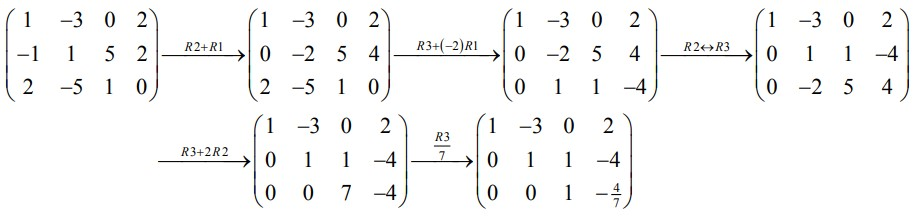
\includegraphics[width=16cm]{images/aug_matrix.jpg}
\end{figure}

By backward substitution, we obtain the solution of the linear system:
\[ x=-\frac{58}{7}, \quad y=-\frac{24}{7}, \quad z=-\frac{4}{7}. \]
\end{proof}

Consider the following two linear systems:
\begin{equation*}\tag{1}
\begin{split}
x + 2y - z + 5w &= -1 \\
y + 3z - w &= 2 \\
z + 2w &= 3 \\
w &= 1
\end{split}
\end{equation*}
and
\begin{equation*}\tag{2}
\begin{split}
x &= 3 \\
y &= 1 \\
z &= 2 \\
w &= 5
\end{split}
\end{equation*}
The solution to (1) can be obtained by backward substitution, while the solution to (2) is immediate.

The augmented matrices of the linear systems (1) and (2) are respectively
\[ \begin{bmatrix}
    1 & 2 & -1 & 5 & -1 \\
    0 & 1 & 3 & -1 & 2 \\
    0 & 0 & 1 & 2 & 3 \\
    0 & 0 & 0 & 1 & 1
\end{bmatrix} \quad \text{and} \quad
\begin{bmatrix}
    1 & 0 & 0 & 0 & 3 \\
    0 & 1 & 0 & 0 & 1 \\
    0 & 0 & 1 & 0 & 2 \\
    0 & 0 & 0 & 1 & 5
\end{bmatrix} \]
The first matrix is an example of a matrix in \textbf{row-echelon form}, while the second matrix is an example of a matrix in \textbf{reduced row-echelon form}.

\begin{defn}{Row-echelon form}{}
A matrix is said to be in \textbf{row-echelon form} if it satisfies all the following properties:
\begin{enumerate}
\item If there are any rows that consist entirely of zeros, then they are grouped together at the bottom of the matrix.
\item If a row does not consist of entirely of zeros, then the first nonzero number in the row is a 1. We call this a leading 1.
\item In any two successive rows that do not consists entirely of zeros, the leading 1 in the lower row occurs further to the right than the leading 1 in the higher row.
\end{enumerate}
The matrix is said to be in \textbf{reduced row-echelon form} if, in addition to the above three properties, the following property is satisfied:
\begin{enumerate}[resume]
\item Each column that contains a leading 1 has zeros everywhere else in that column.
\end{enumerate}
\end{defn}

\begin{exmp}{Linear system with a unique solution}{} 
The augmented matrix of a linear system in $(x,y,z)$ has been reduced to the given row-echelon form:
\[ \begin{bmatrix}
    1 & 2 & -1 & 2 \\
    0 & 1 & 3 & -1 \\
    0 & 0 & 1 & 4
\end{bmatrix} \]
Solve the linear system.
\end{exmp}

\begin{proof}[Solution]
The corresponding linear system is
\begin{align*}
x + 2y - z &= 2 \\
y + 3z &= -1 \\
z &= 4
\end{align*}
By backward substitution, we obtain the solution $x=32$, $y=-13$ and $z=4$.
\end{proof}

\begin{exmp}{Linear system with infinitely many solutions}{}
Write down all the solutions of 
\[ x+2y-z=3. \]
\end{exmp}

\begin{proof}[Solution]
Let $y=s$ and $z=t$, then $x=3-2s+t$.

Thus all the solutions are $x=3-2s+t$, $y=s$ and $z=t$, where $s,t\in\RR$.
\end{proof}

\begin{remark}
Note that $s$ and $t$ are called \textbf{parameters}, and the set of all solutions expressed in terms of the parameters is called the \textbf{general solution} of the linear system.
\end{remark}

\begin{exmp}{}{}
The augmented matrix of a linear system in $(x,y,z,w)$ has been reduced to the reduced-row echelon form:
\[ \begin{bmatrix}
    1 & 0 & 0 & 2 & -7 \\
    0 & 1 & 0 & 1 & 5 \\
    0 & 0 & 1 & 3 & 1 \\
    0 & 0 & 0 & 0 & 0
\end{bmatrix} \]
Solve the linear system.
\end{exmp}

\begin{proof}[Solution]
The corresponding linear system is
\begin{align*}
x + 2w &= -7 \\
y + w &= 5 \\
z + 3w &= 1
\end{align*}
The variables (unknowns) that corresponding to the leading 1's, namely $x$, $y$ and $z$, are called \textbf{leading variables}. The non-leading variables ($w$ in this case) are called \textbf{free variables}.

Solving for leading variables in terms of variables, we can assign any arbitrary value to the free variable $w$, say $t$, which then determines the values of the leading variable. Thus this linear system has \emph{infinitely many solutions} given by
\[ x=-7-2t, \quad y=5-t, \quad z=1-3t, \quad w=t \quad \text{where } t\in\RR \]
\end{proof}

\begin{defn}{Gaussian elimination}{}
The method of solving a linear system by reducing the corresponding augmented matrix to row-echelon form (respectively reduced row-echelon form) is unknown as \textbf{Gaussian elimination} (respectively \textbf{Gauss-Jordan elimination}).
\end{defn}

\begin{exmp}{}{}
Without using a calculator, solve the linear system
\begin{align*}
3x + 4y - 2z + 13w &= 9 \\
x + 2y - 2z + 7w &= 5 \\
2x + y + 4z + 6w &= -3
\end{align*}
\end{exmp}

\begin{proof}[Solution]
We write down the augmented matrix of the linear system and then perform elementary row operations to reduce it to row-echelon form or reduced row-echelon form:
\begin{figure}[H]
    \centering
    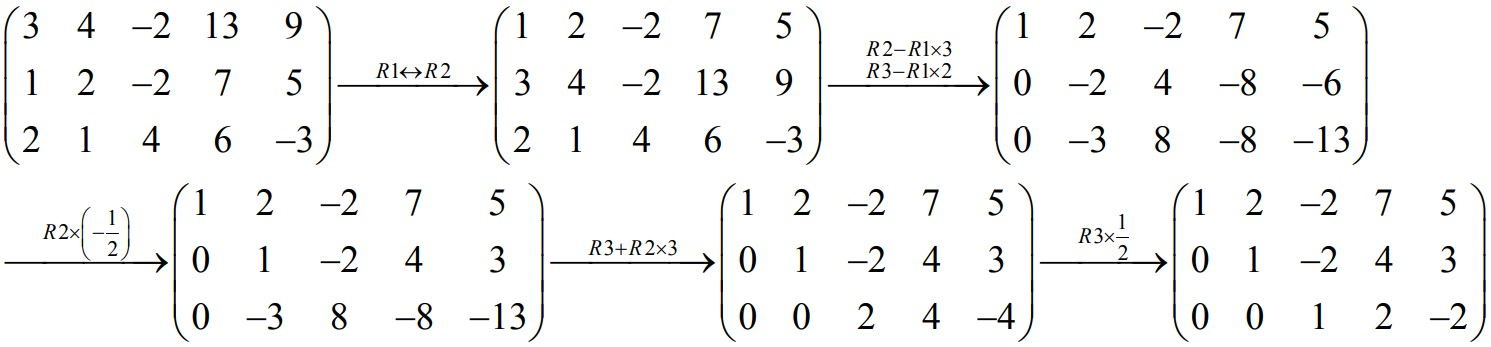
\includegraphics[width=16cm]{images/matrix_1.jpg}
\end{figure}
The linear system corresponding to the row-echelon form is
\begin{align*}
x + 2y - 2z + 7w &= 5 \\
y - 2z + 4w &= 3 \\
z + 2w &= -2
\end{align*}
which has the same set of solutions as the given linear system. Now $x$, $y$ and $z$ are the leading variables, and $w$ is the free variable. Let $w=t$ where $t\in\RR$ is an arbitrary number. By backward substitution, $z=-2-2t, y=-1-8t, x=3+5t$. Thus the general solution of the given linear system is
\[ x=3+5t, \quad y=-1-8t, \quad z=-2-2t, \quad w=t \quad \text{where } t\in\RR \]
Alternatively, we can further reduce the row-echelon form to reduced row-echelon form, then assign $w=t$ to obtain the same general solution.
\end{proof}

\begin{exmp}{Geometrical interpretation}{}
The general solution of the system of linear equations
\begin{align*}
x + y &= -1 \\
2x + y + z &= 3 \\
x + z &= 4
\end{align*}
is given by $x=4-t, y=-5+t, z=t$. What is the geometrical interpretation of the solution?
\end{exmp}

\begin{proof}[Solution]
The three planes $x+y=-1$, $2x+y+z=3$ and $x+z=4$ intersect in a common line, with vector equation
\[ r = \begin{pmatrix} x \\ y \\ z \end{pmatrix} 
= \begin{pmatrix} 4-t \\ -5+t \\ t \end{pmatrix} 
= \begin{pmatrix} 4 \\ -5 \\ 0 \end{pmatrix} + t\begin{pmatrix} -1 \\ 1 \\ 1 \end{pmatrix}, \quad t\in\RR \]
\end{proof}

\subsubsection{Homogenous Linear Systems}
\begin{defn}{Homogenous linear system}{}
A linear system of the form
\[ \begin{split}
a_{11}x_1 + a_{12}x_2 + \cdots + a_{1n}x_n &= 0 \\
a_{21}x_1 + a_{22}x_2 + \cdots + a_{2n}x_n &= 0 \\
&\vdots \\
a_{m1}x_1 + a_{m2}x_2 + \cdots + a_{mn}x_n &= 0
\end{split} \]
is known as a \textbf{homogeneous linear system}.
\end{defn}

Every homogeneous linear system is consistent, since $x_1=x_2=\cdots=x_n=0$ is a solution; this solution is called the \textbf{trivial solution}; if there are other solutions, then they are called \textbf{non-trivial solutions}, i.e. a solution $x_1=s_1, x_2=s_2, \dots, x_n=s_n$ is a non-trivial solution if \emph{at least one} of $s_i \neq 0$.

\begin{thrm}{}{}
Every homogeneous system of linear equations with more unknowns than equations has infinity many solutions.
\end{thrm}

\begin{exmp}{}{}
Determine whether the homogeneous linear system has non-trivial solution.
\begin{align*}
x + y + 3z &= 0 \\
-x + 2y + 6z &= 0 \\
2x - y - 3z &= 0
\end{align*}
\end{exmp}

\begin{proof}[Solution]
The augmented matrix is 
\[ \begin{bmatrix}
    1 & 1 & 3 & 0 \\
    -1 & 2 & 6 & 0 \\
    2 & -1 & -3 & 0
\end{bmatrix} \]
Performing elementary row operations on the augmented matrix gives us:
\[ \begin{bmatrix}
    1 & 1 & 3 & 0 \\
    0 & 3 & 9 & 0 \\\
    0 & 0 & 0 & 0
\end{bmatrix} \]
The corresponding homogeneous system
\begin{align*}
x + y + 3z &= 0 \\
3y + 9z &= 0
\end{align*}
has 3 unknowns and 2 equations.

Hence the homogeneous linear system has non-trivial solution. Since it is equivalent to the given homogeneous system, it also has non-trivial solution.
\end{proof}

% https://en.wikipedia.org/wiki/Matrix_(mathematics)#Linear_equations



\subsection{Linear Transformations}
% https://en.wikipedia.org/wiki/Matrix_(mathematics)#Linear_transformations
• linear spaces and subspaces, and the axioms (restricted to spaces of finite dimension over the field of real numbers only)
• linear independence and span
• basis and dimension (in simple cases), including use of terms such as ‘column space', ‘row space', ‘range space' and ‘null space'
• rank of a square matrix and relation between rank, dimension of null space and order of the matrix
• linear transformations and matrices from $\RR^n$ to $\RR^m$
• eigenvalues and eigenvectors of square matrices (2 × 2 and 3 × 3 matrices, restricted to cases where the eigenvalues are real and distinct)
• diagonalisation of a square matrix M by expressing the matrix in the form QDQ–1, where D is a diagonal matrix of eigenvalues and Q is a matrix whose columns are eigenvectors, and use of this expression such as to find the powers of M 

\subsection{Eigenvalues and Eigenvectors}

\pagebreak

Bases: Spans and Spanning Sets, Linear Independence

Dimension

Linear Transformations

Linear Maps and Matrices

Inner Product Spaces

% remove all from here
\chapter{Vectors}
\section{Basic Properties}
\subsection{Coordinate Space and the Algebra of Vectors}
\begin{defn}{Vector}{}
By a \emph{vector} we will mean a list of $n$ real numbers $x_1,x_2,x_3,\dots,x_n$ where $n$ is a positive integer. Mostly this list will be treated as a row vector and written as
\[ (x_1,x_2,\dots,x_n). \]
Sometimes (for reasons that will become apparent) the numbers will be arranged as a column vector
\[ \begin{pmatrix} x_1\\x_2\\\vdots\\x_n \end{pmatrix}. \]
Often we will denote such a vector by a single letter in bold, say $\vb{x}$, and refer to $x_i$ as the $i$-th coordinate of $\vb{x}$.
\end{defn}

\begin{defn}{Coordinate space}{}
For a given $n$, we denote the set of all vectors with n coordinates as $\RR^n$, and often refer to $\RR^n$ as \emph{$n$-dimensional coordinate space} or simply as \emph{$n$-dimensional space}.
\end{defn}

If $n=2$ then we commonly use $x$ and $y$ as coordinates and refer to $\RR^2=\{(x,y)\mid x,y\in\RR\}$ as the $xy$-plane.

If $n=3$ then we commonly use $x$, $y$ and $z$ as coordinates and refer to $\RR^3=\{(x,y,z)\mid x,y,z\in\RR\}$ as $xyz$-space. 

\begin{remark}
Note that the order of the coordinates matters; so, for example, $(2,3)$ and $(3,2)$ are different vectors in $\RR^2$.
\end{remark}

There is a special vector $(0,0,\dots,0)$ in $\RR^n$ which we denote as $\vb{0}$ and refer to as the \emph{zero vector}.

A vector is an object that has both \emph{magnitude} and \emph{direction}. In simple terms, especially when we are thinking of $\RR^2$ or $\RR^3$, a vector is an arrow. A vector can be used in different ways. Consider the case of vectors in $\RR^3$, the $xyz$-space: we can use a vector to represent a point that has coordinates $x$, $y$ and $z$. We call this vector the \emph{position vector} of that point.

The points $(0,0,\dots,0,x_i,0,\dots,0)$ in $\RR^n$, where $x_i$ is a real number, comprise the $x_i$-axis, with the origin lying at the intersection of all the axes.

Similarly in three (and likewise higher) dimensions, the triple $(x,y,z)$ can be thought of as the point in $\RR^3$ which is $x$ units along the $x$-axis from the origin, $y$ units parallel to the $y$-axis and $z$ units parallel to the $z$-axis, or it can represent the translation which would take the origin to that point.

\begin{defn}{Vector addition}{}
Given two vectors $\vb{u}=(u_1,u_2,\dots,u_n)$ and $\vb{v}=(v_1,v_2,\dots,v_n)$ in $\RR^n$, we can add and subtract them much as you would expect, by separately adding the corresponding coordinates.
That is
\[ \vb{u}+\vb{v}=(u_1+v1, u_2+v2, \dots, u_n+v_n); \quad \vb{u}-\vb{v}=(u_1-v_1, u_2-v_2, \dots, u_n-v_n). \]
\end{defn}

Geometrically, the vector $\vb{u}+\vb{v}$ is constructed by moving the start of the $\vb{v}$ arrow to the end of the $\vb{u}$ arrow: $\vb{u}+\vb{v}$ is then the arrow from the start of $\vb{u}$ to the end of $\vb{v}$.

\begin{defn}{Scalar multiple}{}
Given a vector $\vb{v}=(v_1,v_2,\dots,v_n)$ and a real number $k$ then the scalar multiple $k\vb{v}$ is defined as 
\[ k\vb{v} = (kv_1,kv_2,\dots,kv_n). \]
\end{defn}

We write $-\vb{v}$ for $(-1)\vb{v}=(-v_1,-v_2,\dots,-v_n)$.

\begin{defn}{Standard basis}{}
The $n$ vectors
\[ (1,0,\dots,0), (0,1,0,\dots,0), \dots, (0,\dots,0,1,0), (0,\dots,0,1) \]
in $\RR^n$ are known as the \emph{standard (or canonical) basis} for $\RR^n$. We will denote these, respectively, as $\vb{e}_1,\vb{e}_2,\dots,\vb{e}_n$.
\end{defn}

When $n=2$, the vectors $(1,0)$ and $(0,1)$ form the standard basis for $\RR^2$. These are also commonly denoted by the symbols $\vb{i}$ and $\vb{j}$ respectively. Note that any vector $\vb{v}=(x,y)$ can be written uniquely as a linear combination of $\vb{i}$ and $\vb{j}$: that is $(x,y)=x\vb{i}+y\vb{j}$ and this is the only way to write $(x,y)$ as a sum of scalar multiples of $\vb{i}$ and $\vb{j}$. 

When $n=3$, the vectors $(1,0,0), (0,1,0), (0,0,1)$ form the standard basis for $\RR^3$ being respectively denoted $\vb{i}$, $\vb{j}$, $\vb{k}$.

\subsection{Geometry of Vectors. Some Geometric Theory}
\begin{defn}{Magnitude}{}
The \emph{length (or magnitude)} of a vector $\vb{v}=(v_1,v_2,\dots,v_n)$, denoted by $|\vb{v}|$, is defined by
\[ |\vb{v}| = \sqrt{{v_1}^2+{v_2}^2+\cdots+{v_n}^2}. \]
\end{defn}

We say a vector $\vb{v}$ is a \emph{unit vector} if it has length $1$.

This formula formalises our intuitive idea of a vector as an arrow having a length; the length of the arrow is exactly what you would expect it to be from Pythagoras' Theorem. We see this is the distance of the point $\vb{v}$ from the origin, or equivalently the distance a point moves when it is translated by $\vb{v}$.

So if $\vb{p}$ and $\vb{q}$ are points in $\RR^n$, then the vector that will translate $\vb{p}$ to $\vb{q}$ is $\vb{q}-\vb{p}$, and hence we define:

\begin{defn}{Distance}{}
The distance between two points $\vb{p}$ and $\vb{q}$ in $\RR^n$ is $|\vb{q}-\vb{p}|$ (or equally $|\vb{p}-\vb{q}|$). In terms of their coordinates $p_i$ and $q_i$ we have
\[ |\vb{q}-\vb{p}|=\sqrt{\sum_{i=1}^n(q_i-p_i)^2}. \]
\end{defn}

\begin{remark}
Note that $|\vb{v}|\ge0$ and that $|\vb{v}|=0$ if and only if $\vb{v}=\vb{0}$. Also $|\lambda\vb{v}|=|\lambda|\,|\vb{v}|$ for any real number $\lambda$.
\end{remark}

\begin{thrm}{Triangle Inequality}{}
Let $\vb{u}$ and $\vb{v}$ be vectors in $\RR^n$. Then
\begin{equation}\label{eqn:triangle_inequality}
|\vb{u}+\vb{v}| \le |\vb{u}|+|\vb{v}|
\end{equation}
\end{thrm}

If $\vb{v}\neq\vb{0}$ then there is equality in \cref{eqn:triangle_inequality} if and only if $\vb{u}=\lambda\vb{v}$ for some $\lambda>0$.

\begin{proof}
Let $\vb{u}=(u_1,u_2,\dots,u_n)$ and $\vb{v}=(v_1,v_2,\dots,v_n)$. The inequality \cref{eqn:triangle_inequality} is trivial if $\vb{v}=\vb{0}$, so suppose $\vb{v}\neq\vb{0}$. Note that for any real number $t$,
\[ 0 \le |\vb{u}+t\vb{v}|^2 = \sum_{i=1}^n(u_i+tv_i)^2 = |\vb{u}|^2+2t\sum_{i=1}^nu_iv_i+t^2|\vb{v}|^2. \]
As $|\vb{v}|\neq0$, the RHS of the above inequality is a quadratic in $t$ which is always non-negative, and so has non-positive discriminant ($b^2\le4ac$). Hence
% refer to oxford notes
\end{proof}

\subsection{Equations of lines and planes}
\subsection{The Question Of Consistency}

\section{Vector Product and Vector Algebra}
\subsection{Vector Product}
\subsection{Scalar and vector triple product}
\subsection{Cross product equation of a line}
\subsection{Properties of Determinants}


\section{Vectors}
\subsection{Linear Combinations}
\emph{Linear combinations} of vectors $\vb{u}$ and $\vb{v}$ are given by
\[ \lambda\vb{u}+\mu\vb{v} \]
where $\lambda,\mu\in\RR$.

For $a_1,a_2,a_3\in\RR$, 
\begin{itemize}
\item the combinations $a_1\vb{u}$ fill a \textbf{line} through the origin; 
\item the combinations $a_1\vb{u}+a_2\vb{v}$ fill a \textbf{plane} through the origin; 
\item the combinations $a_1\vb{u}+a_2\vb{v}+a_3\vb{w}$ fill the \textbf{three-dimensional space}. (Provided $\vb{w}$ does not lie in the plane of $\vb{u}$ and $\vb{v}$.)
\end{itemize}

The \textbf{Euclidean space} $\RR^n$, as a set, is defined as the set of vertical vectors with $n$ coordinates in the real numbers. Algebraically, $\RR^n$ is an $n$-dimensional vector space over $\RR$. Vectors in $\RR^n$ are expressed as vertical vectors 
\[ \vb{x} = \begin{pmatrix} x_1 \\ x_2 \\ \vdots \\ x_n \end{pmatrix} \]
To save space, we usually express the above vector compactly as follows:
\[ \vb{x}=(x_1,\dots,x_n) \]

\subsection{Length and Dot Product}
\begin{defn}{Dot product}{}
The dot product (or inner product) of $\vb{v}=(v_1,\dots,v_n)$ and $\vb{w}=(w_1,\dots,w_n)$ is given by
\begin{equation}
\vb{v} \cdot \vb{w} = \sum_{i=1}^nv_iw_i = v_1w_1 + \cdots + v_nw_n
\end{equation}
\end{defn}

It is easy to verify that the dot product is commutative; that is, $\vb{v} \cdot \vb{w} = \vb{w} \cdot \vb{v}$.

For perpendicular vectors, the dot product is zero.

An important case is the dot product of a vector \emph{with itself}. In this case $\vb{v}$ equals $\vb{w}$. The dot product $\vb{v} \cdot \vb{v}$ gives the \textbf{length of $\vb{v}$ squared}.

\begin{defn}{Length}{}
The length $\norm{\vb{v}}$ of a vector $\vb{v}=(v_1,\dots,v_n)$ is the square root of $\vb{v}\cdot\vb{v}$, given by
\begin{equation}
\norm{\vb{v}} = \sqrt{\vb{v}\cdot\vb{v}} = \sqrt{\sum_{i=1}^nv_i^2}
\end{equation}
\end{defn}

\begin{proof}
This simply follows from Pythagoras' theorem.
\end{proof}

The word ``unit” indicates that some measurement equals ``one”. Hence we can define the \textbf{unit vector} as follows.

\begin{defn}{Unit vector}{}
A unit vector of vector $\vb{v}$, denoted by $\hat{\vb{v}}$, is a vector whose length equals one; that is, $\hat{\vb{v}}\cdot\hat{\vb{v}}=1$.
\end{defn}

The standard unit vectors along the $x$- and $y$-axes are written $\hat{\vb{i}}$ and $\hat{\vb{j}}$ respectively. In the $xy$-plane, the unit vector that makes an angle $\theta$ with the $x$-axis is $(\cos\theta,\sin\theta)$.
\[ \hat{\vb{i}}=\begin{pmatrix} 1 \\ 0 \end{pmatrix} \quad \hat{\vb{j}}=\begin{pmatrix} 0 \\ 1 \end{pmatrix} \quad \hat{\vb{u}}=\begin{pmatrix} \cos\theta \\ \sin\theta \end{pmatrix} \]

To get the unit vector, divide any non-zero vector $\vb{v}$ by its length $\norm{v}$.
\begin{equation}
\hat{\vb{v}} = \frac{\vb{v}}{\norm{\vb{v}}}
\end{equation}
is a unit vector in the same direction as $\vb{v}$.

Cosine formula
If $\vb{v}$ and $\vb{w}$ are non-zero vectors then
\begin{equation}
\frac{\vb{v}\cdot\vb{w}}{\norm{\vb{v}}\norm{\vb{w}}} = \cos\theta
\end{equation}
where $\theta$ is the angle between the two vectors.

Since $|\cos\theta|$ never exceeds 1, the cosine formula gives two great inequalities:
\begin{thrm}{Schwarz inequality}{}
\begin{equation}
|\vb{v}\cdot\vb{w}| \le \norm{\vb{v}}\norm{\vb{w}}
\end{equation}
\end{thrm}
\begin{thrm}{Triangle inequality}{}
\begin{equation}
\norm{\vb{v}+\vb{w}} \le \norm{\vb{v}} + \norm{\vb{w}}
\end{equation}
\end{thrm}


\section{Solving Linear Equations}


\chapter{Vector Spaces}
\section{Real and Complex Numbers}
This text assumes that the reader should be familiar with the sets of real and complex numbers, denoted by $\RR$ and $\CC$ respectively.



Euclidean spaces, linear combinations and linear span, subspaces, linear independence, bases and dimension, rank of a matrix, inner products, eigenvalues and eigenvectors, diagonalisation, linear transformations between Euclidean spaces

\section{Definition}
The motivation for the definition of a vector space comes from properties of addition and scalar multiplication in $\FF^n$: Addition is commutative, associative, and has an identity. Every element has an additive inverse. Scalar multiplication is associative. Scalar multiplication by 1 acts as expected. Addition and scalar multiplication are connected by distributive properties. 

We will define a vector space to be a set $V$ with an addition and a scalar multiplication on V that satisfy the properties in the paragraph above.

\begin{defn}{Addition, scalar multiplication}
An \textbf{addition} on $V$ is a function that assigns an element $u+v \in V$ to each pair of elements $u,v \in V$.

A \textbf{scalar multiplication} on $V$ is a function that assigns an element $\lambda v \in V$ to each $\lambda \in \FF$ and each $v \in V$.
\end{defn}

Now we are ready to give the formal definition of a vector space.

\begin{definition}[Vector space]
A \emph{vector space} is a set $V$ along with an addition on $V$ and a scalar multiplication on $V$ such that the following properties hold:
\begin{enumerate}[label=(\roman*)]
\item Commutativity: $\forall u, v \in V, u+v=v+u$
\item Associativity: $\forall u,v,w \in V, u+(v+w)=(u+v)+w$
\item Existence of additive identity: there exists $0 \in V$ such that $\forall v\in V, v + 0 = v = 0 + v$ 
\item Existence of additive inverse: $\forall v \in V$ there exists $w \in V$ such that $v + w = 0_V = w + v$ 
\item Existence of multiplicative identity: $\forall v\in V, 1v = v$
\item Distributivity of scalar multiplication over vector addition: $\forall u,v \in V, \lambda\in\FF, \lambda(u + v) = \lambda u + \lambda v$
\item Distributivity of scalar multiplication over field addition: $\forall v\in V, \lambda,\mu\in\FF, (\lambda+\mu)v = \lambda v + \mu v$
\item Scalar multiplication interacts well with field multiplication: $\forall v\in V, \lambda,\mu\in\FF, (\lambda\mu)v = \lambda(\mu v)$
\end{enumerate}
\end{definition}

Elements of a vector space are called \emph{vectors} or \emph{points}.

The scalar multiplication in a vector space depends on $\FF$. Thus when we need to be precise, we will say that $V$ is a vector space over $\FF$ instead of saying simply that $V$ is a vector space. 

\begin{example}[$\RR^n$ and $\CC^n$]
$\RR^n$ is a vector space over $\RR$, and $\CC^n$ is a vector space over $\CC$.
\end{example}

A vector space over $\RR$ is called a \emph{real vector space}; a vector space over $\CC$ is called a \emph{complex vector space}.

\begin{proposition}[Uniqueness of additive identity]
A vector space has a unique additive identity.
\end{proposition}
\begin{proof}
Suppose $0$ and $0^\prime$ are both additive identities for some vector space $V$.

Then
\[ 0^\prime = 0^\prime + 0 = 0 + 0^\prime = 0 \]
where the first equality holds because $0$ is an additive identity, the second equality comes from commutativity, and the third equality holds because $0^\prime$ is an additive identity. 

Thus $0^\prime = 0$, proving that $V$ has only one additive identity.
\end{proof}

\begin{proposition}[Uniqueness of additive inverse]
Every element in a vector space has a unique additive inverse.
\end{proposition}
\begin{proof}
Suppose $V$ is a vector space. Let $v \in V$. Suppose $w$ and $w^\prime$ are additive inverses of v. Then
\[ w = w+0 = w+(v+w^\prime) = (w+v)+w^\prime = 0+w^\prime = w^\prime \]
Thus $w=w^\prime$, as desired.
\end{proof}

Because additive inverses are unique, the following notation now makes sense.
\begin{notation}
Let $v,w\in V$. Then $-v$ denotes the additive inverse of $v$; $w-v$ is defined to be $w+(-v)$.
\end{notation}

\begin{notation}
For the rest of the book, $V$ denotes a vector space over $\FF$.
\end{notation}

\section{Subspaces}
\begin{definition}[Subspace]
A subset $U \subset V$ is called a subspace of $V$ if $U$ is also a vector space (with the same addition and scalar multiplication as on $V$).
\end{definition}

A subset $U$ of $V$ is a subspace of $V$ if and only if $U$ satisfies the following three conditions:
\begin{enumerate}
\item Existence of additive identity: $0 \in U$
\item Closed under addition: $u+w \in U \implies u+w \in U$
\item Closed under scalar multiplication: $a \in F$ and $u \in U$ implies $au \in U$.
\end{enumerate}
\begin{proof}
If $U$ is a subspace of $V$, then $U$ satisfies the three conditions above by the definition of vector space.

Conversely, suppose $U$ satisfies the three conditions above. The first condition above ensures that the additive identity of $V$ is in $U$.

The second condition above ensures that addition makes sense on $U$. The third condition ensures that scalar multiplication makes sense on $U$.
\end{proof}


\part{Real Analysis}
\chapter{Number Systems}
\section{Natural Numbers $\NN$}
\subsection{Construction}
In Peano's development, it is assumed that there is a set $\NN$ (the natural numbers) of undefined objects with a distinguished element $1$ such that
\begin{enumerate}[label=(\roman*)]
\item $1$ is a natural number; that is $1\in\NN$;
\item every $n\in\NN$ has a successor $S(n)\in\NN$;
\item for every $n$, $S(n)\neq1$ (there is no number with 1 as successor)
\item if $S(n)=S(m)$, then $n=m$;
\item if $A$ is a set of natural numbers such that $1\in A$ and
\[n\in A\implies S(n)\in A,\]
then $A$ contains all natural numbers.
\end{enumerate}

\subsection{Properties}
\begin{theorem}[Archimedean property of $\NN$]
$\NN$ is not bounded above.
\end{theorem}

\begin{proof}
Suppose, for a contradiction, that $\NN$ is bounded above. Then $\NN$ is non-empty and bounded above, so by completeness (of $\RR$) $\NN$ has a supremum.

By the Approximation property with $\epsilon=\frac{1}{2}$, there is a natural number $n\in\NN$ such that $\sup\NN-\frac{1}{2}<n\le\sup\NN$.

Now $n+1\in\NN$ and $n+1>\sup\NN$. This is a contradiction.
\end{proof}
\pagebreak

\section{Rational Numbers $\QQ$}
\subsection{Construction}
\begin{notation}
$\ZZ^\prime=\ZZ\setminus\{0\}$.
\end{notation}

\begin{definition}
Let $\sim$ be the binary relation defined on $\ZZ\times\ZZ^\prime$ by
\[ (a,b)\sim(c,d) \iff ad=bc. \]
\end{definition}

\begin{proposition}
$\sim$ is an equivalence on $\ZZ\times\ZZ^\prime$.
\end{proposition}

\begin{proof}
We just check that $\sim$ is transitive. So suppose that $(a,b)\sim(c,d)$ and $(c,d)\sim(e,f)$. Then
\begin{equation*}\tag{1}
ad=bc
\end{equation*}
\begin{equation*}\tag{2}
cf=de
\end{equation*}
Multiplying (1) by $f$ and (2) by $b$, we obtain
\begin{equation*}\tag{3}
adf=bcf
\end{equation*}
\begin{equation*}\tag{4}
bcf=bde
\end{equation*}
Hence $adf=bde$. Since $d\neq0$, the Cancellation Law implies that $af=bc$. Hence $(a,b)\sim(e,f)$.
\end{proof}

\begin{definition}
The set of \vocab{rational numbers} is defined by
\[ \QQ\coloneqq\ZZ\times\ZZ^\prime/\sim \]
i.e. $\QQ$ is the set of $\sim$ equivalence classes.
\end{definition}

\begin{notation}
For each $(a,b)\in\ZZ\times\ZZ^\prime$, the corresponding equivalence class is denoted by $[(a,b)]$.
\end{notation}

Next we want to define an addition operation on $\QQ$. You may know that
\[\frac{a}{b}+\frac{c}{d}=\frac{ad+bc}{bd}.\]
This suggests we make the following definition:

\begin{definition}
We define the binary operation $+_\QQ$ on $\QQ$ 
by
\[[(a,b)]+_\QQ[(c,d)]=[(ad+bc,bd)].\]
\end{definition}

\begin{remark}
Since $b\neq0$ and $d\neq0$, we have that $bd\neq0$ and so $(ad+bc,bd)\in\ZZ\times\ZZ^\prime$.
\end{remark}

\begin{lemma}
$+_\QQ$ is well-defined.
\end{lemma}

\begin{theorem}
For all $q,r,s\in\QQ$, we have that
\[q+_\QQ r=r+_\QQ q\]
\[q+_\QQ(r+_\QQ s)=(q+_\QQ r)+_\QQ s.\]
\end{theorem}

\begin{definition}[Identity element for $+_\QQ$]
$0_\QQ=[(0,1)]$.
\end{definition}

\begin{proposition}
\begin{enumerate}[label=(\arabic*)]
\item For any $q\in\QQ$, $q+_\QQ0_\QQ=q$.
\item For any $q\in\QQ$, there exists a unique $r\in\QQ$ such that $q+_\QQ r=0_\QQ$.
\end{enumerate}
\end{proposition}

\begin{proof} \
\begin{enumerate}[label=(\arabic*)]
\item Let $q=[(a,b)]$. Then
\begin{align*}
q+_\QQ0Q&=[(a,b)]+_\QQ[(0,1)]\\
&=[(a\cdot1+0\cdot b,b\cdot1)]\\
&=[(a,b)]\\
&=q.
\end{align*}
\item To show that there exists at least one such element, consider $r=[(-a,b)]$. Then
\begin{align*}
q+_\QQ r&=[(a,b)]+_\QQ[(-a,b)]\\
&=[(ab+(-a)b,b^2)]\\
&=[(0,b^2)]
\end{align*}
Since $0\cdot1=0\cdot b^2$, we have $(0,b^2)=(0,1)$. Hence 
\begin{align*}
q+_\QQ r&=[(0,b^2)]\\
&=[(0,1)]\\
&=0_\QQ
\end{align*}
As before, simple algebra shows that there exists at most one such element.
\end{enumerate}
\end{proof}

\begin{definition}
For any $q\in\QQ$, $-q$ is the unique element of $\QQ$ such that
\[q+_\QQ(-q)=0_\QQ.\]
\end{definition}

\begin{definition}
We define the binary operation $-_\QQ$ on $\QQ$ by
\[q-_\QQ r=q+_QQ(-r).\]
\end{definition}

Next we want to define a multiplication operation on $\QQ$. Note that
\[\frac{a}{b}\cdot\frac{c}{d}=\frac{ac}{bd}.\]
This suggests we make the following definition.

\begin{definition}
We define the binary operation $\cdot_\QQ$ on $\QQ$ by
\[[(a,b)]\cdot_\QQ[(c,d)]=[(ac,bd)].\]
\end{definition}

\begin{remark}
Since $b\neq0$ and $d\neq0$, we have that $bd\neq0$ and so $(ac,bd)\in\ZZ\times\ZZ^\prime$.
\end{remark}

\begin{lemma}
$\cdot_\ZZ$ is well-defined.
\end{lemma}

\begin{theorem}
For all $q,r,s\in\QQ$, we have that
\begin{align*}
q\cdot_\QQ r&=r\cdot_\QQ q\\
(q\cdot_\QQ r)\cdot_\QQ s&=q\cdot_\QQ(r\cdot_\QQ s)\\
q\cdot_\QQ(r+_\QQ s)&=(q\cdot_\QQ r)+_\QQ(q\cdot_\QQ s)
\end{align*}
\end{theorem}

\begin{definition}[Identity element for $\cdot_\QQ$]
$1_\QQ=[(1,1)]$.
\end{definition}

\begin{theorem}
\begin{enumerate}[label=(\arabic*)]
\item For all $q\in\QQ$, $q\cdot_\QQ1_\QQ=q$.
\item For every $0_\QQ\neq q\in\QQ$, there exists a unique $r\in\QQ$ such that $q\cdot_\QQ r=1_\QQ$.
\end{enumerate}
\end{theorem}

\begin{proof} \
\begin{enumerate}[label=(\arabic*)]
\item Let $q=[(a,b)]$. Then
\begin{align*}
q\cdot_\QQ1_\QQ
\end{align*}
\end{enumerate}
\end{proof}



\begin{theorem}
$\QQ$ is an ordered set if $r<s$ is defined to mean that $s-r$ is a positive rational number.
\end{theorem}
\pagebreak

\section{Real Numbers $\RR$}
\subsection{Construction: Dedekind cuts}
We shall construct $\RR$ from $\QQ$.

\begin{definition}
A \vocab{Dedekind cut} $\alpha\subset\QQ$ satisfies the following properties:
\begin{enumerate}[label=(\roman*)]
\item $\alpha\neq\emptyset$, $\alpha\neq\QQ$;
\item if $p\in\alpha$, $q\in\QQ$ and $q<p$, then $q\in\alpha$;
\item if $p\in\alpha$, then $p<r$ for some $r\in\alpha$.
\end{enumerate}
\end{definition}

Note that (iii) simply says that $\alpha$ has no largest member; (ii) implies two facts which will be used freely:
\begin{itemize}
\item If $p\in\alpha$ and $q\notin\alpha$ then $p<q$.
\item If $r\notin\alpha$ and $r<s$ then $s\notin\alpha$.
\end{itemize}

\begin{example}
Let $r\in\QQ$ and define
\[ \alpha_r\coloneqq\{p\in\QQ\mid p<r\}. \]
We now check that this is indeed a Dedekind cut.
\begin{enumerate}[label=(\arabic*)]
\item $p=1+r\notin\alpha_r$ thus $\alpha_r\neq\QQ$. $p=r-1\in\alpha_r$ thus $\alpha_r\neq\emptyset$.

\item Suppose that $q\in\alpha_r$ and $q^\prime<q$. Then $q^\prime<q<r$ which implies that $q^\prime<r$ thus $q^\prime\in\alpha_r$.

\item Suppose that $q\in\alpha_r$. Consider $\dfrac{q+r}{2}\in\QQ$ and $q<\dfrac{q+r}{2}<r$. Thus $\dfrac{q+r}{2}\in\alpha_r$.
\end{enumerate}
\end{example}

This example shows that every rational $r$ corresponds to a Dedekind cut $\alpha_r$.

\begin{example}
$\sqrt[3]{2}$ is not rational, but it is real. $\sqrt[3]{2}$ corresponds to the cut
\[ \alpha=\{p\in\QQ\mid p^3<2\}. \]
\begin{enumerate}[label=(\arabic*)]
\item Trivial.
\item If $q<p$, by the monotonicity of the cubic function, this implies that $q^3<p^3<2$ thus $q\in\alpha$.
\item If $p\in\alpha$, consider $\brac{p+\frac{1}{n}}^3<2$.
\end{enumerate}
\end{example}

\begin{definition}
The set of real numbers, denoted by $\RR$, is the set of all Dedekind cuts.
\[ \RR\coloneqq\{\alpha\mid\alpha\text{ is a Dedekind cut}\} \]
\end{definition}

\begin{proposition}
$\RR$ has an order.
\end{proposition}

\begin{proof}
We define $\alpha<\beta$ to mean that $\alpha\subset\beta$. Let us check if this is an order (check for transitivity and trichotomy).
\begin{enumerate}[label=(\arabic*)]
\item For $\alpha,\beta,\gamma\in\RR$, if $\alpha<\beta$ and $\beta<\gamma$ it is clear that $\alpha<\gamma$. (A proper subset of a proper subset is a proper subset.)

\item It is clear that at most one of the three relations
\[ \alpha<\beta, \quad \alpha=\beta, \quad \beta<\alpha \]
can hold for any pair $\alpha,\beta$. 

To show that at least one holds, assume that the first two fail. Then $\alpha$ is not a subset of $\beta$. Hence there exists some $p\in\alpha$ with $p\in\beta$.

If $q\in\beta$, it follows that $q<p$ (since $p\notin\beta$), hence $q\in\alpha$, by (ii). Thus $\beta\subset\alpha$. Since $\beta\neq\alpha$, we conclude that $\beta<\alpha$.
\end{enumerate}
Thus $\RR$ is an ordered set.
\end{proof}

\begin{proposition}
The ordered set $\RR$ has the least-upper-bound property.
\end{proposition}

\begin{proof}
Let $A\neq\emptyset$, $A\subset\RR$. Assume that $\beta\in\RR$ is an upper bound of $A$.

Define $\beta$ to be the union of all $\alpha\in A$; in other words, $p\in\gamma$ if and only if $p\in\alpha$ for some $\alpha\in A$. We shall prove that $\gamma\in\RR$ by checking the definition of Dedekind cuts:
\begin{enumerate}[label=(\arabic*)]
\item Since $A$ is not empty, there exists an $\alpha_0\in A$. This $\alpha_0$ is not empty. Since $\alpha_0\subset\gamma$, $\gamma$ is not empty.

Next, $\gamma\subset\beta$ (since $\alpha\subset\beta$ for every $\alpha\in A$), and therefore $\gamma\neq\QQ$.

\item Pick $p\in\gamma$. Then $p\in\alpha_1$ for some $\alpha_1\in A$. If $q<p$, then $q\in\alpha_1$, hence $q\in\gamma$.

\item If $r\in\alpha_1$ is so chosen that $r>p$, we see that $r\in\gamma$ (since $\alpha_1\subset\gamma$).
\end{enumerate}

Next we prove that $\gamma=\sup A$.
\begin{enumerate}[label=(\arabic*)]
\item It is clear that $\alpha\le\gamma$ for every $\alpha\in A$.
\item Suppose $\delta<\gamma$. Then there is an $s\in\gamma$ and that $s\notin\delta$. Since $s\in\gamma$, $s\in\alpha$ for some $\alpha\in A$. Hence $\delta<\alpha$, and $\delta$ is not an upper bound of $A$.
\end{enumerate}
\end{proof}

\begin{proposition}
$\RR$ is closed under addition.
\end{proposition}

\begin{proof}
Let $\alpha = (A,B)$, $\beta = (C,D)$, then $\alpha + \beta = (X,Y)$ where
\[ X = \{a+c \mid a \in A, c \in C\} \]

To show that $(X,Y)$ is a Dedekind cut, we simply need to check the conditions for Dedekind cuts. 
\begin{itemize}
\item Property 1 is trivial.

\item Property 2 is by definition.

\item Property 3:

Let $x,y \in X$ satisfy $x<y$, $y \in X$. 

Let $y = a + c$, $a \in A$, $c \in C$.

Let $\epsilon = y - x$.

Let $a^\prime = a - \dfrac{\epsilon}{2}$, $c^\prime = c - \dfrac{\epsilon}{2}$.

Then \[ a^\prime + c^\prime = a + c - \epsilon = x \]
$a^\prime < a, a \in A \implies a^\prime \in A$. Similarly, $c^\prime \in C$.\\
$\therefore\:x = a^\prime +c^\prime \in X$.

\item Property 4:

$\forall a+c \in X, a \in A, c \in C$, $\exists a^\prime \in A, c^\prime \in C$ such that $a<a^\prime, c<c^\prime$.

$\therefore\:a^\prime +c^\prime \in X$ satisfies $a+c < a^\prime+c^\prime$.
\end{itemize}
\end{proof}

We now prove that the set of real numbers satisfies the commutative, associative, and identity field axioms with respect to addition.

\begin{proposition}
Addition is commutative on $\RR$: $\forall\alpha,\beta\in\RR$,
\[ \alpha+\beta=\beta+\alpha \]
\end{proposition}

\begin{proof}
We need to show that $\alpha+\beta\subseteq\beta+\alpha$ and $\beta+\alpha\subseteq\alpha+\beta$.

Let $r\in\alpha+\beta$. Then $r=a+b$ for $a\in\alpha$ and $b\in\beta$. Thus $r=b+a$ since $+$ is commutative on $\QQ$. Hence $r\in\beta+\alpha$. Therefore $\alpha+\beta\subseteq\beta+\alpha$.

Similarly, $\beta+\alpha\subseteq\alpha+\beta$.

Therefore $\alpha+\beta=\beta+\alpha$.
\end{proof}

\begin{proposition}
Addition is associative on $\RR$: $\forall\alpha,\beta,\gamma\in\RR$,
\[ \alpha+(\beta+\gamma)=(\alpha+\beta)+\gamma. \]
\end{proposition}

\begin{proof}
Let $r\in\alpha+(\beta+\gamma)$. Then $r=a+(b+c)$ where $a\in\alpha,b\in\beta,c\in\gamma$. Thus $r=(a+b)+c$ by associativity of $+$ on $\QQ$. Therefore $r\in(\alpha+\beta)+\gamma$, hence $\alpha+(\beta+\gamma)\subseteq(\alpha+\beta)+\gamma$.

Similarly, $(\alpha+\beta)+\gamma\subseteq\alpha+(\beta+\gamma)$.
\end{proof}

\begin{proposition}
Define $0^*\coloneqq\{p\in\QQ\mid p<0\}$. Then $\alpha+0^*=\alpha$.
\end{proposition}

\begin{proof}
Let $r\in\alpha+0^*$. Then $r=a+p$ for some $a\in\alpha,p\in0^*$. Thus $r=a+p<a+0=a$ by ordering on $\QQ$ and identity on $\QQ$. Hence $\alpha+0^*\subseteq\alpha$.

Let $r\in\alpha$. Then there exists $r^\prime>p$ where $r^\prime\in\alpha$. Thus $r-r^\prime<0$, so $r-r^\prime\in0^*$. We see that
\[ r=\underbrace{r^\prime}_{\in\alpha}+\underbrace{(r-r^\prime)}_{\in0^*}. \]
Hence $\alpha\subseteq\alpha+0*$.
\end{proof}

%%%%%%%%%%%%%%%%

\begin{exercise}
Express $-\alpha$ in terms of $\alpha$; show
\[ \alpha+(-\alpha)=0=(-\alpha)+\alpha \]
\end{exercise}

\begin{proof}
We split this into two cases.

\textbf{Case 1}: $\alpha$ is a rational number, then $\alpha=(A,B)$ where $A = \{x \mid x < \alpha\}$, $B = \{x \mid x \ge \alpha\}$.

Let $-\alpha=(A^\prime,B^\prime)$, where $A^\prime = \{x \mid x < -\alpha\}$, $B^\prime = \{x \mid x\ge -\alpha\}$. 
We see that $\alpha+(-\alpha) \le 0$ is obvious.

On the other hand, since $0=(O,O^\prime)$, for any $\epsilon<0$ we have
\[ \epsilon = \brac{\alpha+\frac{\epsilon}{2}} + \brac{-\alpha+\frac{\epsilon}{2}} \in A+A^\prime \]
Hence $\alpha+(-\alpha)=0$.

\

\textbf{Case 2}: $\alpha$ is irrational, let $\alpha = (A,B)$ where $B$ does not have a lowest value. 
Then $-B = \{-x \mid x \in B\}$ does not have a highest value.

We wish to define $-\alpha=(-B,-A)$, but first we need to show that this is well-defined by checking through all the conditions.

\begin{itemize}
\item Property 1: This is trivial.

\item Property 2: Prove that $- A$ and $B$ are disjoint.

Note that $\forall x \in \RR$, if $x=-y$, then exactly one out of $y \in A$ and $y \in B$ is true $\implies$ exactly one out of $x \in -B$ and $x \in -A$ is true.

\item Property 3: Prove $-B$ is closed downwards.

Suppose otherwise, that $x<y, y \in -B$ but $x \notin -B$. Then $-y \in B$, $-x \notin B$. Since $A$ is the complement of $B$, $-y \notin A$, $-x \in A$. But $-y<-x$, which is a contradiction.

\item Property 4 is already guaranteed by the irrationality of $\alpha$.
\end{itemize}

All of these properties imply that the real numbers form a commutative group by addition.
\end{proof}

\subsubsection{Negation}
Given any set $X \subset \RR$, let $-X$ denote the set of the negatives of those rational numbers. That is $x \in X$ if and only if $-x \in -X$. 

If $(A,B)$ is a Dedekind cut, then $-(A,B)$ is defined to be
$(-B,-A)$.

This is pretty clearly a Dedekind cut. - proof

\subsubsection{Signs}
A Dedekind cut $(A,B)$ is \textbf{positive} if $0 \in A$ and \textbf{negative} if $0 \in B$. If $(A,B)$ is neither positive nor negative, then $(A,B)$ is the cut representing 0.

If $(A,B)$ is positive, then $-(A,B)$ is negative. Likewise, if $(A,B)$ is negative, then $-(A,B)$ is positive. The cut $(A,B)$ is non-negative if it is either positive or 0.

\subsubsection{Multiplication}
% Define multiplication of real numbers; you will need to define them for positive real numbers first

%\subsubsection{Positive multiplication}
Let $\alpha = (A,B)$ and $\beta = (C,D)$ where $\alpha, \beta$ are both non-negative.

We define $\alpha \times \beta$ to be the pair $(X,Y)$ where

$X$ is the set of all products $ac$ where $a \in A, c \in C$ and at least one of the two numbers is non-negative. 
$Y$ is the set of all products $bd$ where $b \in B, d \in D$.

%\subsubsection{General Multiplication}


% https://www.math.brown.edu/reschwar/INF/handout3.pdf

\subsection{Properties}
\begin{theorem}[$\RR$ is archimedian]\label{thrm:r-archimedian}
For any $x\in\RR^+$ and $y\in\RR^+$, there exists some $n\in\ZZ^+$ so that
\[n\cdot x>y.\]
\end{theorem}

\begin{proof}
In particular, if we take $x=1$ from this theorem, we immediately get the following statement.

\begin{proposition}\label{prop:r-archimedian}
For any $y\in\RR$, there exists some positive integer $n$ so that $n>y$.
\end{proposition}

We now give a proof of Proposition \ref{prop:r-archimedian} directly without using Theorem \ref{thrm:r-archimedian}, and then we prove Theorem \ref{thrm:r-archimedian} from Proposition \ref{prop:r-archimedian}. This shows that these two statements are in fact equivalent, though Proposition \ref{prop:r-archimedian} looks much simpler.

\begin{proof}
Assume $n\in\ZZ^+$ does not exist; that is to say that the set of positive integers $\ZZ^+$ has an upper bound $y$. Then using the l.u.b. property of $\RR$, $\sup\ZZ^+$ exists, which we denote by $x_0\in\RR$.

Now we look at $x_0-1$. This is not an upper bound by definition of $x_0$, which means there exists some $N\in\ZZ^+$ such that
\[x_0-1<N.\]
Then it follows that $x_0<N+1$. Notice that $N+1\in\ZZ^+$. So this contradicts the assumption that $x_0$ is an upper bound.

Hence our original assumption cannot be true, and thus there exists $n\in\ZZ^+$ with $n>y$.
\end{proof}

For any $x\in\RR^+$ and $y\in\RR$, consider $y\cdot x^{-1}\in\RR$. From Proposition \ref{prop:r-archimedian}, there exists some $n\in\ZZ^+$ such that
\[n>y\cdot x^{-1}.\]
Then this is equivalent to $n-yx^{-1}>0$. Since $x>0$, and $\RR$ is an ordered field, we have
\[(n-y\cdot x^{-1})\cdot x>0.\]
This is equivalent to $n\cdot x>y$.
\end{proof}

\begin{remark}
The archimedian property guarantees that we can use decimals to represent real numbers. %See Rudin 1.22
\end{remark}

% https://mth32015.files.wordpress.com/2015/01/jan-26-30.pdf

\begin{theorem}[$\QQ$ is dense in $\RR$]
For any $a,b\in\RR$ with $a<b$, there exists some $x\in\QQ$ such that $a<x<b$.
\end{theorem}

\begin{proof}
This means one can find some $m\in\ZZ$ and $n\in\ZZ^+$ so that
\[a<\frac{m}{n}<b,\]
which is further equivalent to finding $m\in\ZZ$ and $n\in\ZZ^+$ so that
\[an<m<bn.\]
Notice that $b-a>0$, so by the archimedian property, there exists $n\in\ZZ^+$ so that
\[bn-an=(b-a)n>1.\]
We now argue that there exists some integer between two real numbers, whenever their difference is larger than 1.

\begin{lemma*}
For any $\alpha,\beta\in\RR$ with $\beta-\alpha>1$, there exists some integer $m$ so that $\alpha<m<\beta$.
\end{lemma*}

\begin{proof}
We prove this lemma by finding such $m$. First, using archimedian property of $\RR$, we can find some integer $N>0$ so that
\[-N<\alpha<\beta<N.\]
Then consider the integers which are smaller than $N$ and greater than $\alpha$, i.e., the set
\[A\coloneqq\{k\in\ZZ\mid a<k\le N\}.\]
It is not empty since $N\in A$. Since this a subset of $\{-N+1,-N+2,\dots,N-2,N-1,N\}$ which is a finite set, it contains only finite elements. We can pick the smallest one from it and denote it by $m$, i.e., $m\coloneqq\min A$. We claim this $m$ is just the one we are looking for.

First since $m\in A$, $m>\alpha$. Then we only need to check $m<\beta$. If this is not true, i.e., $m\ge\beta$, then we consider $m-1$. It follows
\[m-1\ge\beta-1\ge\alpha.\]
This contradicts the fact that $m$ is the smallest integer which is greater than $\alpha$.

Above all, we are done with the lemma.
\end{proof}

At last, apply the lemma to $\alpha=an$ and $\beta=bn$, we are done.
\end{proof}

\begin{theorem}[$\RR$ is closed under taking roots]
For every $y\in\RR^+$ and every $n\in\ZZ^+$, there exists a unique $x\in\RR^+$ so that $x^n=y$.
\end{theorem}

\begin{proof}
We first claim that such $x\in\RR^+$, if exists, must be unique. Otherwise, assume that both $x_1,x_2\in\RR^+$ are solutions of the equation
\[x^n=y,\quad y\in\RR^+,n\in\ZZ^+.\]
Assume now $x_1<x_2$, then from the fact that $\RR$ is an ordered field, we have $x_1^n<x_2^n$ (why?), a contradiction. Similarly, $x_1>x_2$ also leads to a contradiction, and so $x_1=x_2$.

Now we look for a solution for the equation. Consider a subset of $\RR$ as
\[S\coloneqq\{a\in\RR^+\mid a^n<y\}.\]
Try to check that
\begin{enumerate}[label=(\arabic*)]
\item $S\neq\emptyset$;
\item $S$ has an upper bound.
\end{enumerate}
Then using the fact that $\RR$ has the l.u.b. property, $\sup S$ exists. Define it as $x$, clearly $x\in\RR^+$. We show that $x$ solves the equation. (The idea of the proof is similar to the proof of $\sup_\QQ\{x\in\QQ\mid x^2\le2\}$ does not exist.)

First, we show that if $x^n<y$, then we can construct some $x_0\in S$ which is greater than $x$, which says $x$ is not an upper bound of $S$. So $x^n\ge y$.

Second, we show that if $x^n>y$, then we can find an upper bound of $S$ which is smaller than $x$, which says that $x$ is not the least upper bound. So $x^n\le y$.

Above all, we must have $x^n=y$.

From now on, we use $y^\frac{1}{n}$ to denote the unique solution for the equation
\[x^n=y,\quad y\in\RR^+,n\in\ZZ^+,\]
and call it the $n$-th real root of $y$. The property
\[(ab)^\frac{1}{n}=a^\frac{1}{n}\cdot b^\frac{1}{n}\]
immediately follows from the uniqueness of $n$-th real root.
\end{proof}

\begin{theorem}[Completeness axiom for $\RR$]
If non-empty $E\subset\RR$ is bounded above, then $E$ has a supremum.
\end{theorem}

Any set in the reals bounded from above/below must have a supremum/infimum.

\begin{proof}
We prove this using Dedekind cuts.

Let $S$ be a real number set. 
We consider the rational number set $A = \{x \in \QQ \mid \exists y \in S\}$. Set $B$ is defined to be the complement of $A$ in $\QQ$.

We go through the definitions to check that $(A|B)$ is a Dedekind cut.
\begin{enumerate}
\item Since $S \neq \emptyset$, pick $y \in S$, then $[y]-1$ is a real number smaller than some element in $S$, hence $[y]-1 \in A$ and thus $A \neq \emptyset$.

Since we're given that $S$ is bounded, $\exists M>0$ as the upper bound for $S$, thus $B \neq \emptyset$.

(Note that an upper bound is simply a number that is bigger than anything from the set, and is not the supremum

\item We defined $B$ to be the complement of $A$ in $\QQ$, so this condition is trivial.

\item For any $x,y \in A$, if $x<y$ and $y\in A$, then $\exists z \in S$ such that $y<z \implies x<z \implies x \in A$.

\item Suppose otherwise that $x \in A$ is the largest element in A, then $\exists y \in S$ such that $x<y$
We then pick a rational number $z$ between $x$ and $y$. 
Since we still have $z<y$, we have $z \in A$ but $z>x$, contradictory to $z$ being the largest.

Now there's actually an issue with the proof for property 4 here
How exactly are we finding z?

First $x \in \QQ$. 
Then $y \in \RR$ so we rewrite it as $y=(C|D)$ via definition.

$x<y$ translates to the fact that $x \in C$.

Since $y$ is real, by definition we know that $C$ must not have a largest element.

In particular, $x$ is not largest and we can pick $z \in C$ such that $z>x$. 
This is in fact the $z$ that we need
\end{enumerate}

Now that all the properties of a real number are validated, we may finally conclude that $\alpha=(A|B)$ is indeed a real number.

Now we need to show that $\alpha = \sup S$.

Let $x \in S$. 
If $x$ is not the maximum value of $S$, i.e. $\exists y \in S,x<y$, then $x \in A$ and thus $x<\alpha$.

If $x$ is the maximum value of $S$, then for any rational number $y<x$ we have $y \in A$, and for any rational number $y \ge x$ we have $y \in B$.
Thus $x=(A|B)=\alpha$.

In conclusion, $x \le \alpha$ for all $x \in S$.

For any upper bound $x$ of $S$, since $\forall y \in S, x \ge y$ we have $x \in B$ and thus $x \ge \alpha$.

$\therefore$ $\alpha$ is the smallest upper bound of $S$ and thus $\sup S = \alpha$ exists.
\end{proof}

\subsection{Extended real number system}
\begin{definition}
We add $\pm\infty$ to $\RR$, and call the union $\RR\cup\{\pm\infty\}$ the \vocab{extended real number system}. Now any non-empty set $E\subset\RR$ has a supremum and infimum, since we can define
\[\sup E=+\infty,\quad\text{if $E$ has no upper bound in $\RR$}\]
and
\[\inf E=-\infty,\quad\text{if $E$ has no lower bound in $\RR$.}\]
\end{definition}

The extended real number system does not form a field, but it is customary to make the following conventions:
\begin{enumerate}[label=(\arabic*)]
\item If $x$ is real then
\[ x+\infty=+\infty, \quad x-\infty=-\infty, \quad \frac{x}{+\infty}=\frac{x}{-\infty}=0. \]
\item If $x>0$ then $x\cdot(+\infty)=+\infty$, $x\cdot(-\infty)=-\infty$.
\item If $x<0$ then $x\cdot(+\infty)=-\infty$, $x\cdot(-\infty)=+\infty$.
\end{enumerate}
When it is desired to make the distinction between real numbers on the one hand and the symbols $+\infty$ and $-\infty$ on the other quite explicit, the former are called \emph{finite}.
\pagebreak

\section{Euclidean Plane $\RR^2$}
We consider the Cartesian product of $\RR$ with $\RR$; that is,
\[ \RR^2\coloneqq\RR\times\RR\coloneqq\{(x_1,x_2)\mid x_1,x_2\in\RR\}. \]
Over $\RR^2$, we can define operations
\begin{itemize}
\item Addition $+$: $(x_1,x_2)+(y_1,y_2)=(x_1+y_1,x_2+y_2)$;
\item Scalar multiplication $\RR\times\RR^2\to\RR^2$: $c\cdot(x_1,x_2)=(c\cdot x_1,c\cdot x_2)$.
\end{itemize}

This two operations make $\RR^2$ a 2-dimensional vector space (linear space) over the real field $\RR$. We also say $\RR^2$ is a $\RR$-linear space of real dimension 2. For example, $\{(1,0),(0,1)\}$ form a basis of $\RR^2$.

Moreover, over the linear space $\RR^2$, one can define an inner product as
\[ \langle(x_1,x_2),(y_1,y_2)\rangle=x_1y_1+x_2y_2. \]
The inner product induces a norm
\[ |(x_1,x_2)|=\sqrt{\langle(x_1,x_2),(x_1,x_2)\rangle}=\sqrt{x_1^2+x_2^2}. \]
From now on, we use $\vec{x}$ to denote $(x_1,x_2)$.
\begin{proposition} \
\begin{itemize}
\item $|\vec{x}|\ge0$, where equality holds if and only if $\vec{x}=\vec{0}$.
\item $|c\cdot\vec{x}|=|c||\vec{x}|$
\item $|\vec{x}+\vec{y}|\le|\vec{x}|+|\vec{y}|$
\item $|\langle\vec{x},\vec{y}\rangle|\le|\vec{x}||\vec{y}|$
\end{itemize}
\end{proposition}

All constructions here can be easily generalised to any $\RR^n$ with $n\in\ZZ^+$.

\section{Complex Numbers $\CC$}


Over $\RR^2$, we can define a multiplication $\cdot$ as
\[ (a,b)\cdot(c,d)=(ac-bd,ad+bc). \]
If we identity $\RR^2$ with
\[ \CC\coloneqq\{x+yi\mid x,y\in\RR\} \]
via $(x,y)\mapsto x+yi$, then all structures defined above are induced to $\CC$. In particular, the multiplication is induced to $\CC$ via requiring $i^2=-1$. A nontrivial fact is that $(\CC,+,\cdot)$ is a field. A element in $\CC$ is called a complex number. Usually, people prefer to use $z=x+yi$, $x,y\in\RR$, to denote a complex number. Here $x$ is called the real part of $z$ and $y$ is called the imaginary part of $z$. We use $|z|$ to denote its norm.
\pagebreak

\section{Euclidean Spaces}
For each positive integer $n$, let $\RR^n$ be the set of all ordered $n$-tuples
\[ \vb{x}=(x_1,x_2,\dots,x_n), \]
where $x_1,\dots,x_n$ are real numbers, called the \emph{coordinates} of $\vb{x}$. The elements of $\RR^n$ are called points, or vectors, especially when $n>1$. We shall denote vectors by boldfaced letters.

Since $\RR^n$ is a vector space (over $\RR$), $\RR^n$ has the following extra properties
\begin{itemize}
\item For any two vectors $\vb{x}$ and $\vb{y}$ we may perform addition:
\[ \vb{x}+\vb{y}=(x_1+y_1,\dots,x_n+y_n) \]
Properties of addition:
\begin{enumerate}
\item $\vb{x}+\vb{y}=\vb{y}+\vb{x}$
\item $(\vb{x}+\vb{y})+\vb{z}=\vb{x}+(\vb{y}+\vb{z})$
\item Zero vector $\vb{0}=(0,\dots,0)$ satisfies $\vb{x}+\vb{0}=\vb{0}+\vb{x}=\vb{x}$
\item For any vector $\vb{x}$, its negative $-\vb{x}$ satisfies $\vb{x}+(-\vb{x})=(-\vb{x})+\vb{x}=\vb{0}$
\end{enumerate}
\item For any vector $\vb{x}$ and scalar $k\in\RR$ we may perform scalar multiplication:
\[ k\vb{x}=(kx_1,\dots,kx_n) \]
Properties of scalar multiplication:
\begin{enumerate}
\item $0\cdot\vb{x}=\vb{0},1\cdot\vb{x}=\vb{x}$
\item $(kl)\vb{x}=k(l\vb{x})=l(k\vb{x})$
\item $k(\vb{x}+\vb{y})=k\vb{x}+k\vb{y}$
\item $(k+l)\vb{x}=k\vb{x}+l\vb{x}$
\end{enumerate}
\end{itemize}

We define the \textbf{inner product} (or scalar product) of $\vb{x}$ and $\vb{y}$ by
\[ \vb{x}\cdot\vb{y}\coloneqq\sum_{i=1}^nx_iy_i. \]

The Euclidean space builds upon the vector space $\RR^n$; specifically speaking, it is $\RR^n$ endowed with two extra notions:
\begin{itemize}
\item The \textbf{norm} of the Euclidean space $\norm{\cdot}$ is a real-valued function $\norm{\cdot}:\RR^n\to\RR$. Given a vector $\vb{x}=(x_1,\dots,x_n)$ in $\RR^n$, the norm of $\vb{x}$ is defined as
\[ \norm{\vb{x}}\coloneqq\sqrt{\vb{x}\cdot\vb{x}}=\sqrt{\sum_{i=1}^nx_i^2}=\sqrt{x_1^2+\cdots+x_n^2}. \]
\item The \textbf{metric} $d$ of the Euclidean space is a real-valued function $d:\RR^n\times\RR^n\to\RR$. Given two vectors $\vb{x}=(x_1,\dots,x_n)$ and $\vb{y}=(y_1,\dots,y_n)$, the distance between $\vb{x}$ and $\vb{y}$ is defined as
\[ d(\vb{x},\vb{y})\coloneqq\norm{\vb{x}-\vb{y}}=\sqrt{\sum_{i=1}^n(x_i-y_i)^2}=\sqrt{(x_1-y_1)^2+\cdots+(x_n-y_n)^2}. \]
\end{itemize}

\begin{remark}
The norm is something like the length of the vector itself (distant to the origin); the metric refers to the distance function which measures the length between two points in $\RR^n$ (determined by their positional vectors $\vb{x}$ and $\vb{y}$). Essentially, the metric is a much more general notion than the norm: the norm can only be defined on vector spaces; the metric can literally be defined on any set.
\end{remark}

Norms are required to satisfy the following properties:
\begin{enumerate}[label=(\arabic*)]
\item (\textbf{positive definiteness}) for any vector $\vb{x}$, $\norm{\vb{x}}\ge0$, and equality holds if and only if $\vb{x}=\vb{0}$.
\item (\textbf{absolute homogeneity}) for any vector $\vb{x}$ and scalar $a$, $\norm{a\vb{x}}=|a|\norm{\vb{x}}$.
\item (\textbf{triangle inequality}) for any two vectors $\vb{x}$ and $\vb{y}$, $\norm{\vb{x}+\vb{y}}\le\norm{\vb{x}}+\norm{\vb{y}}$.
\end{enumerate}

Metrics are required to satisfy the following properties:
\begin{enumerate}[label=(\arabic*)]
\item (\textbf{positive definiteness}) for any two elements $\vb{x}$ and $\vb{y}$, $d(\vb{x},\vb{y})\ge0$, equality holds if and only if $\vb{x}=\vb{y}$.
\item (\textbf{symmetry}) for any two elements $\vb{x}$ and $\vb{y}$, $d(\vb{x},\vb{y})=d(\vb{y},\vb{x})$.
\item (\textbf{triangle inequality}) for any three elements $\vb{x}$, $\vb{y}$ and $\vb{z}$, $d(\vb{x},\vb{z})\le d(\vb{x},\vb{y})+d(\vb{y},\vb{z})$.
\end{enumerate}

Generally, if there is a norm $\norm{\cdot}$ on some vector space, then this norm naturally determines a metric $d(x,y)=\norm{x-y}$, which is precisely the case for Euclidean spaces.

\begin{definition}
$E\subset\RR^n$ is \vocab{bounded} if there exists $M>0$ such that $\norm{x}\le M$ for all $x\in E$.
\end{definition}

\begin{exercise}
Given $E$ and $F$ in $\RR^n$ and real number $k$, define
\[ kE=\{kx \mid x\in E\} \]
\[ E+F=\{x+y \mid x\in E,y\in F\} \]
\begin{enumerate}[label=(\alph*)]
\item Show that if $E$ is bounded, then $kE$ is bounded;
\item Show that if $E$ and $F$ are bounded, then $E+F$ is bounded.
\end{enumerate}
\end{exercise}

\begin{definition}
The \vocab{diameter} of $E\subset\RR^n$ is defined as
\[ \diam E\coloneqq\sup_{x,y\in E}d(x,y). \]
\end{definition}

\begin{exercise}
Find the diameter of the open unit ball in $\RR^n$ given by
\[ B=\{x\in\RR^n \mid \norm{x}<1\}. \]
\end{exercise}

\begin{solution}
First note that
\[ d(x,y)=\norm{x-y}\le\norm{x}+\norm{-y}=\norm{x}+\norm{y}<1+1=2. \]
On the other hand, for any $\epsilon>0$, we pick
\[ x=\brac{1-\frac{\epsilon}{4},0,\dots,0}, \quad y=\brac{-\brac{1-\frac{\epsilon}{4}},0,\dots,0}. \]
Then $d(x,y)=2-\dfrac{\epsilon}{2}>2-\epsilon$.

Therefore $\diam B = 2$.
\end{solution}

\begin{exercise}
Given a set $E$ in $\RR^n$, show that $E$ is bounded iff $\diam E<+\infty$.
\end{exercise}
\begin{proof} \

($\implies$) If $E$ is bounded, then there exists $M>0$ such that $\norm{x}\le M$ for all $x \in E$.

Thus for any $x,y \in E$,
\[ d(x,y)=\norm{x-y}\le\norm{x}+\norm{y}\le2M. \]
Thus $\diam E = \sup d(x,y) \le 2M<+\infty$.

($\impliedby$) Suppose that $\diam E=r$. Pick a random point $x \in E$, suppose that $\norm{x}=R$.

Then for any other $y \in E$,
\[ \norm{y}=\norm{x+(y-x)}\le\norm{x}+\norm{y-x}\le R+r. \]
Thus, by picking $M=R+r$, we obtain $\norm{y}\le M$ for all $y \in E$, and we are done.

\begin{remark}
Basically you use $x$ to confine $E$ within a ball, which is then confined within an even bigger ball centered at the origin.
\end{remark}
\end{proof}

\begin{definition}
The \vocab{distance between sets} $E\subset\RR^n$ and $F\subset\RR^n$ is defined as
\[ d(E,F)\coloneqq\inf_{x\in E,y\in F}\norm{x-y}. \]
\end{definition}

Obviously $d(E,F)>0$ implies that $E$ and $F$ are disjoint, but $E$ and $F$ may still be disjoint even if $d(E,F)=0$. For example, the closed intervals $E=(-1,0)$ and $F=(0,1)$.

\begin{exercise}
Suppose that $E$ and $F$ are sets in $\RR^n$ where $E$ and $F$ is finite. Prove that $E$ and $F$ are disjoint iff $d(E,F)>0$.
\end{exercise}

\chapter{Basic Topology}
\section{Metric Space}
\begin{definition}
A set $X$, whose elements we shall call \emph{points}, is a \vocab{metric space} if for any two points $p,q\in X$ there is associated a real value function (called distance function or \emph{metric}) $d:X\times X\to\RR$ which satisfies the following properties:
\begin{enumerate}[label=(\roman*)]
\item (\textbf{positive definitiveness}) $d(p,q)\ge0$, where equality holds if and only if $x=y$;
\item (\textbf{symmetry}) $d(p,q)=d(q,p)$;
\item (\textbf{triangle inequality}) $d(p,q)\le d(p,r)+d(r,q)$ for any $r\in X$.
\end{enumerate}
\end{definition}

\begin{example}
The most important examples of metric spaces are the euclidean spaces $\RR^n$, especially $\RR^1$ (the real line) and $\RR^2$ (the complex plane); the distance in $\RR^n$ is defined by
\[ d(\vb{x},\vb{y})=|\vb{x}-\vb{y}|. \]
\end{example}

A metric space $(X,d)$ naturally induces a metric on any of its subsets.

\begin{definition}
For any $x\in X$, $r>0$, the subset $B_r(x)\coloneqq\{y\in X\mid d(y,x)<r\}$ is called the \vocab{open ball} centred at $x$ with radius $r$.

Similarly, the subset $\bar{B}_r(x)\coloneqq\{y\in X\mid d(y,x)\le r\}$ is called the \vocab{closed ball} centred at $x$ with radius $r$.
\end{definition}

An open ball centred at $x$ is also called a \vocab{neighbourhood} of $x$.

\begin{example}
An open (closed) ball in $\RR$ is equivalent to a finite open (closed) interval, i.e. $(a,b)$ ($[a,b]$), $a,b\in\RR$.
\end{example}

\begin{definition}
Let $X$ be a metric space. All points and sets mentioned below are understood to be elements and subsets of $X$.
\begin{enumerate}[label=(\arabic*)]
\item $p$ is a \vocab{limit point} of $E$ if every neighborhood of $p$ contains $q\neq p$ such that $q\in E$:
\[ \forall r>0,\exists q\in E, q\neq p\suchthat q\in B_r(p). \]
The \vocab{induced set} of $E$, denoted by $E^\prime$, is the set of all limit points of $E$ in $X$.
\item $p$ is an \vocab{isolated point} of $E$ if it not a limit point of $E$.
\item $E$ is \vocab{closed} if every limit point of $E$ is a point of $E$, i.e $\bar{E}=E$.

The \vocab{closure} of $E$, denoted by $\bar{E}$, is the union set $E\cup E^\prime$.

\item $p$ is an \vocab{interior point} of $E$ if there is a neighborhood $N$ of $p$ such that $N\subset E$:
\[ \exists r>0 \suchthat B_r(p)\subset E. \]
The \vocab{interior} of $E$, denoted by $E^\circ$, is the set of all interior points in $E$:
\[E^\circ\coloneqq\{p\in X\mid \exists r>0 \suchthat B_r(p)\subset E\}\]
A point $x$ is an \vocab{exterior point} of $A$ if it is an interior point of $A^c$.
\item $E$ is \vocab{open} if every point of $E$ is an interior point of $E$, i.e. $E^\circ=E$.
\item $E$ is \vocab{perfect} if $E$ is closed and if every point of E is a limit point of $E$.
\item $E$ is \vocab{bounded} if 
\[ \exists M\in\RR, q\in X\suchthat\forall p\in E, d(p,q)<M. \]
The \vocab{boundary} of $E$, denoted by $\partial E$, is the set difference $\bar{E}\setminus E^\circ$.

$p$ is a \vocab{boundary point} of $E$ if $p\in\partial E$.

$E$ is compact if it is a bounded closed set.
\item $E$ is \vocab{dense} in $X$ if every point of $X$ is a limit point of $E$, or a point of $E$ (or both). 

A subset $B\subset A$ is a dense subset of $A$ if $\bar{B}=A$.

$E$ is \vocab{nowhere dense} its closure has no interior, i.e. $(\bar{E})^\circ=\emptyset$.
\end{enumerate}
\end{definition}

\begin{proposition}
Any open ball is open.
\end{proposition}

\begin{proof}
Assume $B_r(x)$ is an open ball in a metric space $(X,d)$. Then for any point $y\in B_r(x)$, there is
\[ d(y,x)<r. \]
Now we define $r^\prime\coloneqq r-d(y,x)$, which is positive.

Consider the ball $B_{r^\prime}(y)$. We shall show it lives in $B_r(x)$. For this, take any point $z\in B_{r^\prime}(y)$. Using the triangle inequality of a metric, we have
\begin{align*}
d(z,x)&\le d(z,y)+d(y,x)\\
&<r^\prime+d(y,x)\\
&=r.
\end{align*}
Hence $z\in B_r(x)$, and $B_{r^\prime}(y)\subset B_r(x)$.
\end{proof}

\begin{proposition}
\begin{enumerate}[label=(\arabic*)]
\item Both $\emptyset$ and $X$ are open.
\item If $S_1,S_2$ are open, then $S_1\cap S_2$ is open.
\item For any set $\Lambda$ such that for any $\alpha\in\Lambda$, $S_\alpha$ is an open subset of $X$, the union $\bigcup_{\alpha\in\Lambda}S_\alpha$ is open.
\end{enumerate}
\end{proposition}

\begin{proof} \
\begin{enumerate}[label=(\arabic*)]
\item Obvious by definition.
\item Take a point $x\in S_1\cap S_2$, we need to find an open ball with radius $r>0$ such that $x\in B_r(x)\subset S_1\cap S_2$.

To find such $r>0$, notice that since both $S_1$ and $S_2$ are open, there are open balls
\begin{align*}
&x\in B_{r_1}(x)\subset S_1\\
&x\in B_{r_2}(x)\subset S_2
\end{align*}
Take $r\coloneqq\min\{r_1,r_2\}$. Then $B_r(x)\subset B_{r_1}(x)\subset S_1$ and $B_r(x)\subset B_{r_2}(x)\subset S_2$, and hence $B_r(x)\subset S_1\cap S_2$.

\item Take a point $x\in\bigcup_{\alpha\in\Lambda}S_\alpha$, then we can assume $x$ lives in some $S_{\alpha_0}$, $\alpha_0\in\Lambda$. Since $S_{\alpha_0}$ is open, take an open ball 
\[ B_r(x)\subset S_{\alpha_0}. \]
It follows
\[ B_r(x)\subset S_{\alpha_0}\subset\bigcup_{\alpha\in\Lambda}S_\alpha. \]
Hence $\bigcup_{\alpha\in\Lambda}S_\alpha$ is open.
\end{enumerate}
\end{proof}

\begin{example}
We know $I_n\coloneqq\brac{-\frac{1}{n},\frac{1}{n}}\subset\RR$ is open for any $n\in\ZZ^+$. However, $\bigcap_{n\in\ZZ^+}I_n=\{0\}$ is not open.
\end{example}

\begin{proposition}
\begin{enumerate}[label=(\arabic*)]
\item Both $\emptyset$ and $X$ are closed.
\item If $S_1$ and $S_2$ are closed, then $S_1\cup S_2$ is closed.
\item For any set $\Lambda$ so that any $\alpha\in\Lambda$, $S_\alpha$ is a closed subset of $X$, the intersection $\bigcap_{\alpha\in\Lambda}S_\alpha$ is closed.
\end{enumerate}
\end{proposition}

\begin{proof} \
\begin{enumerate}[label=(\arabic*)]
\item It follows immediately from $\emptyset=X^c$ and $X=\emptyset^c$.
\item It follows from above that
\[ (S_1\cup S_2)^c=S_1^c\cap S_2^c \]
is open, and hence $S_1\cup S_2$ is closed.
\item It follows from above that
\[ \brac{\bigcap_{\alpha\in\Lambda}S_\alpha}^c=\bigcup_{\alpha\in\Lambda}S_\alpha^c \]
is open, and hence $\bigcap_{\alpha\in\Lambda}S_\alpha$ is closed.
\end{enumerate}
\end{proof}

\begin{proposition}
If $p$ is a limit point of $E$, then every neighbourhood of $p$ contains infinitely many points of $E$.
\end{proposition}

\begin{proof}
Prove by contradiction. Suppose there is a neighborhood $B_r(p)$ which contains only a finite number of points of $E$: $q_1,\dots,q_n$, which are distinct from $p$. Define
\[ r=\min_{1\le m\le n} d(p,q_m). \]
The minimum of a finite set of positive numbers is clearly positive, so that $r>0$.

The neighborhood $B_r(p)$ contains no point $q\in E,q\neq p$ so that $p$ is not a limit point of $E$, a contradiction.
\end{proof}

\begin{corollary}
A finite point set has no limit points.
\end{corollary}

\begin{proposition}
$E$ is open if and only if its complement $E^c$ is closed.
\end{proposition}

\begin{proof} \

($\implies$) Suppose $E$ is open. Let $x$ be a limit point of $E^c$. Then every neighbourhood of $x$ contains a point of $E^c$, so that $x$ is not an interior point of $E$. Since $E$ is open, this means that $x\in E^c$. It follows that $E^c$ is closed.

($\impliedby$) Suppose $E^c$ is closed. Choose $x\in E$. Then $x\notin E^c$, and $x$ is not a limit point of $E^c$. Hence there exists $B_r(x)$ such that $E^c\cap B_r(x)$ is empty, that is, $B_r(x)\subset E$. Thus $x$ is an interior point of $E$, and $E$ is open.
\end{proof}

\begin{proposition}
\begin{enumerate}[label=(\arabic*)]
\item $\bar{E}$ is closed;
\item $E=\bar{E}$ if and only if $E$ is closed;
\item $\bar{E}\subset F$ for every closed set $F\subset X$ such that $E\subset F$.
\end{enumerate}
By (1) and (3), $\bar{E}$ is the \emph{smallest} closed subset of $X$ that contains $E$.
\end{proposition}

\begin{proof} \
\begin{enumerate}[label=(\arabic*)]
\item 
\item 
\item 
\end{enumerate}
\end{proof}

\begin{proposition}
\begin{enumerate}[label=(\arabic*)]
\item $E^\circ$ is open.
\item $E$ is open if and only if $E=E^\circ$.
\item If $G\subset E$ and $G$ is open, then $G\subset E^\circ$.
\end{enumerate}
\end{proposition}

\begin{proof} \
\begin{enumerate}[label=(\arabic*)]
\item If $p\in E^\circ$ then $B_r(p)\subset E$ for some $r>0$ and if $q\in B_r(p)$ then by triangle inequality, $B_{r-d(p, q)}(q)\subset E$ so $B_r(p)\subset E^\circ$ and
hence $E^\circ$ is open.

\item Certainly if $E$ is open then $E=E^\circ$ since for each $p\in E$ there exists $r>0$ such that $B_r(p)\subset E$.

Conversely if $E^\circ=E$ then this holds for each $p\in E$ so $E$ is open.

\item If $G\subset E$ is open then for each $p\in G$ there exists $r>0$ such that
$B_r(p)\subset G$, hence $B_r(p)\subset E$ so $p\in E^\circ$ and it follows that $G\subset E^\circ$.
\end{enumerate}
\end{proof}

\begin{proposition}
The set of exterior points, $(A^c)^\circ$ is the same as $(\bar{A})^c$.
\end{proposition}

\begin{proof}
\begin{align*}
x \in (A^c)^\circ 
&\iff \exists \epsilon>0 \text{ such that } B(x,\epsilon) \subset A^c \\
&\iff B(x,\epsilon) \cap A = \emptyset \\
&\iff x \notin A \text{ and } B_0(x,\epsilon) \cap A=\emptyset \\
&\iff x \notin A \cup A^\prime = \bar A \\
&\iff x \in (\bar A^c)
\end{align*}
\end{proof}

\begin{proposition}
\begin{enumerate}[label=(\arabic*)]
\item $A^\prime$ is closed.
\item $\bar{A}$ is closed, i.e. bar(barA)=barA
\end{enumerate}
\end{proposition}

\begin{proof} \
\begin{enumerate}[label=(\arabic*)]
\item In order to show that $A^\prime$ is closed, we need to show that if $x$ is a limit point of $A^\prime$, then $x\in A^\prime$, i.e. $x$ is a limit point of $A$.

So we need to show that limit points of $A^\prime$ are always limit points of $A$: 
Let $x$ be a limit point of $A^\prime$, then for all $\epsilon>0$, $B_0(x,\epsilon/2)$ intersects with $A^\prime$ and we may pick $y \in B_0(x,\epsilon/2)\cap A^\prime$

Now here's the tricky part
Since $y \in A^\prime$, y is a limit point of $A$, hence $B_0(y,|y-x|)$ intersects with $A$ and thus we may pick $z \in B_0(y,|y-x|)\cap A$.

We show that $z \in B_0(x,\epsilon)$:
\[ |z-x|\le|z-y|+|y-x|<2|y-x|<\epsilon, \]
hence $z \in B(x,\epsilon)$.
\[ |z-y|<|x-y|, \]
hence $z \neq x$

$\therefore\:z \in B_0(x,\epsilon)$

\item 
\end{enumerate}
\end{proof}

Prove the following properties regarding dense sets:

1. $A$ is a dense set in $X$ if and only if $A$ intersects with all open sets in $X$.
2. If $A$ is dense in $X$ and $B$ is dense in $A$, then $B$ is dense in $X$
3. If $A$ and $B$ are dense in $X$ where $A$ is open, then $A\cap B$ is dense in $X$

Ex 5: Regarding closures (The following properties are relatively nontrivial compared to its 'open-set' counterparts):
1. $A^{\prime\prime}=A^\prime$
2. $\bar{A}$ is closed, i.e. $\bar{\bar{A}}=\bar{A}$

%%%%%%%%%%%%%%%%%%%%%%%%

\begin{theorem}[Cantor's Intersection Theorem]
Given a decreasing sequence of compact sets $A_1\supset A_2 \supset \cdots$, there exists a point $x\in\RR^n$ such that $x$ belongs to all $A_i$. In other words, $\bigcap_{i=1}^\infty A_i\neq\emptyset$. Moreover, if for all $i\in\NN$ we have $\diam A_{i+1}\le c\cdot\diam A_k$ for some constant $c<1$, then such a point must be unique, i.e. $\bigcap_{i=1}^\infty A_k=\{x\}$ for some $x\in\RR^n$.
\end{theorem}

\begin{theorem}[Heine--Borel Theorem]
A set $A\subset\RR^n$ is compact if and only if every open covering has a finite subcover, i.e. for any family of open sets $\mathscr{U}=\{U_i\}_{i\in I}$ satisfying $A\subset\bigcup_{i\in I}U_i$, there exists $\{U_1,\dots,U_n\}\subset\mathscr{U}$ such that $A\subset\bigcup_{i=1}^n U_i$.
\end{theorem}

\begin{theorem}[Bolzano--Weierstrass Theorem]
Infinite bounded sets in $\RR^n$ must contain limit points.
\end{theorem}

We will follow a very specific sequence of steps to prove these three theorems:
\begin{enumerate}[label=(\alph*)]
\item Cantor Intersection for $n=1$
\item Bolzano--Weierstrass for $n=1$
\item Bolzano--Weierstrass for general $n$
\item Cantor Intersection for general $n$
\item Heine--Borel for general $n$
\end{enumerate}

\begin{proof} \
\begin{enumerate}[label=(\alph*)]
\item Suppose that there is a decreasing sequence of compact sets $A_1, A_2, \dots$ in the real numbers

Since $A_k$ are bounded, we may let $a_k=\inf A_k$
Also since $A_k$ are closed, $a_k \in A_k$

Note that since $A_k$ is a decreasing sequence of sets we have $a_1\le a_2\le\dots$

Also, whenever we have $n>k$, we have $a_n \in A_n$, but $A_n \subset A_k$ and thus $a_n \in A_k$.

Let $b_1=\sup A_1$, then $a_k \in A_1$ and thus $a_k\le b_1$ for all $k$.

This tells us that the sequence $\{a_k\}$ is bounded above, and thus we may let $a=\sup a_k$.

Our goal is to show that the number $a$ appears in all $A_k$, thus showing that the entire intersection $\bigcap A_k$ contains $a$ and thus must be non-empty.

Now we split this in two cases, which asks whether a is simply made from isolated points, or if it is actually some nontrivial point obtained from the boundaries of $A_k$

\textbf{Case 1:} $a_k=a$ for some $k$
In this case we see that $a_k\le a_n\le a$ for all $n>k$ and thus $a_n=a$ in this case, therefore a is an element in $A_n$ for all $n$

In this case you can imagine that there is a possibility where a is an isolated minimum point of $A_n$ which stays there forever in the decreasing sequence of sets

\textbf{Case 2:} $a_k<a$ for all $k$; in this case we see that $a$ is the limit point of the increasing sequence $\{a_k\}$

Exercise 1: Show that $a$ is a limit point of each $A_k$.

Note that $a_n$ is in $A_k$ for each $n>k$, and since $a=\sup\{a_k\}$ where $a_k$ is increasing, we can actually show that a is a limit point of $\{a_n \mid n \le k\}$:
For every $\epsilon>0$, we pick $n_0$ such that $0 < a-a_{n_0} < \epsilon$
Pick $n\prime > \max\{k,n_0\}$, then $a_{n^\prime} \ge a_{n_0}$ and so
\[ 0<a-a_n\prime \le a_{n_0} < \epsilon \]
This shows that there exists $a_n^\prime$ in $B_0(a,\epsilon) \cap \{a_n \mid n>k\}$ for all $\epsilon$, and so $a$ is a limit point of $\{a_n \mid n>k\}$.

Now since $\{a_n|n \ge k\}$ is a subset of $A_k$ we also see that a is a limit point of $A_k$
Finally, since $A_k$ is closed, we conclude that $a$ is in $A_k$ for all $k$, and we are done

Wait hold on, I forgot about the second part

Now we consider a decreasing sequence of compact sets $A_1, A_2, \dots$ such that $\diam A_{k+1} \le c \diam A_k$ for $c<1$.

Suppose otherwise that there exists $x, y$ in $\bigcap A_k$

You can imagine that this will form a fixed distance between two points, and thus there is a constant positive lower bound for the diameters:
\[ \diam A_k \ge |x-y| > 0 \forall k \]

But this cannot be true because $\diam A_{k+1} \le c \diam A_k$ and so the diameter is controlled by a decreasing geometric sequence:
\[ \diam A_{k+1} \le c^k \diam A_1 \]

So we can simply pick a natural number $k$ such that
\[ k > \log_c \frac{|x-y|}{\diam A_1} \]

\item We consider an infinite bounded set $A$ in the real numbers. Since $A$ is bounded, we can pick a closed interval $[a_1,b_1]$ containing $A$.

We then perform a series of binary cuts: Consider the two halves of $[a_1,b_1]$. We know that at least one of these two must contain infinitely many elements in $A$, otherwise $A$ cannot be infinite. We pick this half of the interval and denote it by $[a_2,b_2]$. We continue this to pick a decreasing sequence of closed intervals $[a_n,b_n]$.

Now $\diam [a_{n+1},b_{n+1}] = \frac{1}{2} \diam [a_n,b_n]$, so by the Cantor Intersection Theorem, there exists a unique real number $c$ in the intersection $\bigcap[a_n,b_n]$.

We show that this $c$ is in fact a limit point of $A$.

For any $\epsilon>0$, we need to show that $B_0(c,\epsilon) \cap A \neq \emptyset$, i.e. we need to find an element $x \neq c$ in $A$ that is less than $\epsilon$ apart from $c$.

We then realize that we can simply exploit the decreasing sequence $[a_n,b_n]$
Since $\diam [a_n,b_n]$ is controlled by a decreasing sequence:
\[ \diam [a_{n+1},b_{n+1}] \le 1/2^n \diam [a_1,b_1] \]
We take a sufficiently large n so that $b_n-a_n<\epsilon$
Since $c$ is in $[a_n,b_n]$, for all $x$ in $[a_n,b_n]$ we have $|x-c|\le b_n-a_n<\epsilon$ and therefore $[a_n,b_n]$ is within $B(c,\epsilon)$.

Here's the funny part: $[a_n,b_n]$ contains infinitely many elements of $A$, so it must contain at least one element in A that is not $c$.

Therefore this element $x \neq c$ is in $B_0(c,\epsilon)$.

\item Now we have an infinte bounded set $A$ in $\RR^n$

The idea here is to consecutively come up with better and better sequences of points in $A$. We denote $x_i$ to be the $i$-th coordinate in $\RR^n$.

Our first wish is to pick some elements in $A$ so that they sort of converge at $x_1$.

Because such considerations of 'restricting to a single coordinate' is important here, we define the projection map to the $i$-th coordinate by
\[ f_i(x_1,\dots,x_n)=x_i \]

So, we look at $f_i(A)$ and try to apply BW for the case where $n=1$.

However, the problem is that $f_i(A)$ need not be infinite. For example, the set $\{(0,0),(0,1),(0,2),\dots\}$ projected onto the first coordinate is simply $\{0\}$.

This forces us to consider two cases

Exercise 2: Show that $f_i(A)$ is bounded
This is simple
1. $f_1(A)$ is infinite, then we can apply BW(n=1) to find a real number $c_1$ which is a limit point in $f_1(A)$

Here we can construct a sequence of points 
\[ \{x^{(1),1},x^{(1),2},...\} \]
so that their first coordinates satisfy
\[ |x^{(1),n}_1-c_1| < 1/n \]
for all natural number n
(I know this notation is cumbersome but the problem is that we need multiple sequences for this proof)

2. $f_1(A)$ is finite, then by the Pigeonhole Principle there exists a real number $c_1$ such that its preimage $f_1^{-1}(c_1)$ in $A$ is infinite

In this case we can randomly pick a sequence $\{x^{(1),1},x^{(1),2},\dots\}$ in $A$ so that their first coordinate is equal to $c_1$

I forgot to mention something that is implied, but we actually do have the need to emphasize that the sequence $\{x^{(1),1},x^{(1),2},\dots\}$ can be chosen to contain mutually distinct entries

Now that we have a sequence that behaves nice on the first coordinate, we may then move on to the second coordinate

Let $A_1=\{x^{(1),1},x^{(1),2},\dots\}$
We again consider $f_2(A_1)$ in two cases, infinite or finite

In any case, we are able to find a subsequence $\{x^{(2),1},x^{(2),2},\dots\}$, where
$x^{(2),k}=x^{(1),n_k}$ for some strictly increasing sequence of natural numbers $n_k$

So that, for the limit point/point with infinite preimage $c_2$, this sequence satisfies
\[ |f_2(x^{(2),n})-c_2| < \frac{1}{n} \]
Note that the property we have for the second case (we in fact have $f_2(x^{(2),n})=c_2$) is just a better version of this.

Now, take note that picking this subsequence does no harm whatsoever towards the first coordinate (if anything it would turn out to be better) since
\[ |f_1(x^{(2),k})-c_1| = |f_1(x^{(1),n_k}-c_1| < \frac{1}{n_k} \le \frac{1}{k} \]
($n_1<\dots<n_k$ is a strictly increasing sequence of natural numbers so $n_k \ge k$)

This continues on until we obtain a sequence of points $\{x^{(n),1},x^{(n),2},\dots\}$ in $A$ so that
\[ |f_i(x^{(n),k}-c_i|<\frac{1}{k} \quad \forall i,k \]

As we can see, the point $c=(c_1,\dots,c_n)$ is in fact a limit point of $A$ as we can always choose a big enough $k$ so that $x^{(n),k}$ is in $B(c,\epsilon) \cap A$.

Since $\{x^{(n),k}\}$ was always chosen to be a sequence of distinct entries, there is no danger for this sequence to always be c, and so c must be a limit point of $A$.

\item We may now return to the general case of Cantor.

Suppose that there is a sequence of decreasing compact sets $A_1,A_2,\dots$ in $\RR^n$. 
Note that every point is contained in $A_1$, so boundedness will never be an issue here.

Since $A_k$ are all nonempty, we can simply pick any element $a_k$ from $A_k$.

For the uncannily specific case that there are only finitely many $\{a_k\}$ chosen, we simply note that, again by Pigeonhole Principle, one of the $a_k$ appears infinitely often; thus for each $A_n$ we simply pick $n_k>n$ so that $A_{n_k}$ contains $a_k$, then $a_k$ is in $A_{n_k}$ which is a subset of $A_n$.

Otherwise, we can then note that $\{a_k\}$ is an infinite bounded set of points, so there must exist a limit point a of $\{a_k\}$.

We can now see that $a$ is always an element of $A_k$:
Using the same technique as Exercise 1, we see that a is a limit point of $\{a_n \mid n>k\}$ and so is a limit point of $A_k$, therefore a is in $A_k$ as $A_k$ is closed.

This proves the first part of the statement
The second part is completely identical to the second part of the $n=1$ case so we don't need to waste our time there either

\item We now consider a compact set A with some open covering $\mathscr{U}$.

This theorem is proved by contradiction: 
Suppose otherwise that set $A$ cannot be covered by any finite collection of open sets in $\mathscr{U}$

Since $A$ is compact, we may enclose it in a closed cube $Q_1$ (whose edges are parallel to the axes)

Now, for each step, we partition $Q$ into $2^n$ cubes by cutting it in half from each direction.

Then, starting from $Q_1$, there must exist one of these smaller cubes, denoted by $Q_2$, such that $A \cap Q_2$ cannot be covered by a finite collection of open sets in $\mathscr{U}$. 
Otherwise, if each $A \cap Q$ has a finite cover, then we simply collect all of these open sets together to form a finite cover of $A$, which violates our assumption.

We continue on to partition $Q_n$ and pick $Q_{n+1}$ so that $A_{n+1}$ has no finite cover (denote $A_n = A \cap Q_n$).

Note that $A$ and $Q_n$ are both compact, so $A_n$ is compact
Also we see that there is a decreasing sequence $A_1,A_2,\dots$
(we can't exactly obtain a relation between $\diam A_n$ and $\diam A_{n+1}$ here)

By Cantor Intersection Theorem we can always find a point $x$ in $A$ located in the intersection $\bigcap A_k$.

Now, since $\mathscr{U}$ is an open covering of $A$, there exists an open set $U$ in $\mathscr{U}$ such that $x\in U$.

The final key step is to exploit the sequence of decreasing cubes $Q_n$. So even though there isn't a clear cut way to control the sizes of $\diam A_n$, we do in fact have the property that $\diam Q_{n+1} = \frac{1}{2^n} \diam Q_1$.

Therefore, by picking a sufficiently large $n$, we can obtain $Q_n$ that is contained in $U$.

But this is a contradiction. 
This is because we've specifically chosen the sequence $A_n$ to be sets that do not possess any finite cover $\{U_1,...,U_n\}$ in $\mathscr{U}$. But here $A_n$ simply would have a one-element cover $\{U\}$.

This completes our proof.
\end{enumerate}
\end{proof}

\begin{comment}
\begin{enumerate}
\item An arbitrary union of open sets is open; a finite intersection of open sets is open.

\begin{proof}
Let $A$ be an arbitrary union of open sets $\{U_i\}_{i \in I}$.

Then for any $x \in A$, suppose that $x \in U_i$, then since $U_i$ is open we can pick $B(x,\epsilon)$ subset of $U_i$ subset of $A$

On the other hand, let $U$ and $V$ be open sets and let $x \in U \cap V$. 
Since $U$ and $V$ are open, we can pick $\epsilon_1$ and $\epsilon_2$ such that $B(x,\epsilon_1)$ is in $U$ whereas $B(x,\epsilon_2)$ is in $V$. 
Then we simply pick $\epsilon=\min\{\epsilon_1,\epsilon_2\}$ so that $B(x,\epsilon)$ is in $U \cap V$.
\end{proof}

\item An arbitrary intersection of closed sets is closed; a finite union of closed sets is closed.

\begin{proof}
This follows from de Morgan's Law on P1 and P2.
\end{proof}
\end{enumerate}
\end{comment}

\section{Compactness}
\begin{definition}
By an \vocab{open cover} of a set $E$ in a metric space $X$ we mean a collection $\{G_\alpha\mid\alpha\in\Lambda\}$ of open subsets of $X$ such that
\[ E\subset\bigcup_{\alpha\in\Lambda}G_\alpha. \]
For $\Lambda^\prime\subset\Lambda$, if the subcollection $\{G_\alpha\mid\alpha\in\Lambda^\prime\}$ is also an open cover of $S$; that is,
\[ E\subset\bigcup_{\alpha\in\Lambda^\prime}U_\alpha, \]
then $\{G_\alpha\mid\alpha\in\Lambda^\prime\}$ is called a \vocab{subcover}. If moreover, $\Lambda^\prime$ is finite, then it is called a \vocab{finite subcover}.
\end{definition}

\begin{definition}
A subset $K$ of metric space $X$ is said to be \vocab{compact} if every open cover of $K$ contains a finite subcover.
\end{definition}

\begin{proposition}
Suppose $K\subset Y\subset X$. Then $K$ is compact relative to $X$ if and only if $K$ is compact relative to $Y$.
\end{proposition}

\begin{proof} \

($\implies$) Suppose $K$ is compact relative to $X$. Let $\{V_\alpha\mid\alpha\in\Lambda\}$ be a collection of sets open relative to $Y$, such that $K\subset\bigcup_{\alpha\in\Lambda}V_\alpha$. By 
\end{proof}

sequential compactness
A set $K$ is compact if and only if every sequence of points in $K$ has a subsequence that converges to a point in $K$.

Any continuous function defined on a compact set is bounded.

extreme value theorem

\section{Perfect Sets}


\section{Connected Sets}
\begin{definition}
Two subsets $A$ and $B$ of a metric space $X$ are said to be \vocab{separated} if both $A\cap\bar{B}$ and $\bar{A}\cap B$ are empty, i.e. no point of $A$ lies in the closure of $B$ and no point of $B$ lies in the closure of $A$.

A set $E\subset X$ is said to be \vocab{connected} if $E$ is not a union of two non-empty separated sets. 
\end{definition}

\begin{remark}
Separated sets are of course disjoint, but disjoint sets need not be separated. For example, the interval $[0,1]$ and the segment $(1,2)$ are not separated, since $1$ is a limit point of $(1,2)$. However, the segments $(0,1)$ and $(1,2)$ are separated.
\end{remark}

The connected subsets of the line have a particularly simple structure: 

\begin{proposition}
A subset $E\subset\RR^1$ is connected if and only if it has the following property: if $x,y\in E$ and $x<z<y$, then $z\in E$.
\end{proposition}

\begin{proof}
($\impliedby$) If there exists $x,y\in E$ and some $z\in(x,y)$ such that $z\notin E$, then $E=A_z\cup B_z$ where
\[ A_z=E\cap(-\infty,z), \quad B_z=E\cap(z,\infty). \]
Since 

($\implies$) 
\end{proof}

\chapter{Numerical Sequences and Series}
\section{Convergent Sequences}
\begin{definition}
A sequence $\{x_n\}$ in a metric spaec $X$ is said to \vocab{converge} if there exists some $x\in X$ such that $\forall\epsilon>0$, $\exists N\in\NN$, $\forall n>N$, 
\[ d(x_n,x)<\epsilon. \]

We denote it as 
\[ \lim_{n\to\infty}x_n=x, \]
and call $x$ the \vocab{limit} of the sequence $\{x_n\}$.

If $\{x_n\}$ does not converge, it is said to \vocab{diverge}.
\end{definition}

\begin{remark}
Take note of the use of logical statements:
\begin{itemize}
\item $\epsilon$ is independent, so it is literally for all $\epsilon>0$.
\item $N$ is dependent on $\epsilon$; if $\epsilon$ is very small we would expect the sequence $\{x_n\}$ to get close enough to $x$ further down the line.
\item The order of the quantifiers matters.
\end{itemize}
\end{remark}

\begin{example}
$\dfrac{1}{n}\to 0$ as $n\to\infty$. The proof is fairly straighforward: $\forall\epsilon>0$, pick $N=\frac{1}{\epsilon}+1$. Then $\forall n>N$,
\[ \frac{1}{n}<\frac{1}{N}=\frac{1}{\frac{1}{\epsilon}+1}<\frac{1}{\frac{1}{\epsilon}}=\epsilon. \]
\end{example}

We now outline some important properties of convergent sequences in metric spaces.

\begin{proposition}
Let $\{x_n\}$ be a sequence in a metric space $X$.
\begin{enumerate}[label=(\arabic*)]
\item $\{x_n\}$ converges to $x\in X$ if and only every neighbourhood of $x$ contains $x_n$ for all but finitely many $n$.
\item (uniqueness of the limit) If $x\in X$, $x^\prime\in X$, and if $\{x_n\}$ converges to $x$ and to $x^\prime$, then $x^\prime=x$.
\item (boundedness of convergent sequences) If $\{x_n\}$ converges, then $\{x_n\}$ is bounded.
\item If $E\subset X$ and if $x$ is a limit point of $E$, then there is a sequence $\{x_n\}$ in $E$ such that $\displaystyle x=\lim_{n\to\infty}x_n$.
\end{enumerate}
\end{proposition}

\begin{proof} \
\begin{enumerate}[label=(\arabic*)]
\item ($\implies$) Suppose $\{x_n\}$ converges to $x$, we wish to prove: given any neighbourhood $U$ of $x$, $U$ eventually contains all $x_n$.

Since $U$ is a neighbourhood of $x$, we pick a ball of radius $\epsilon$ centered at $x$, $B_\epsilon(x)$, so that $B_\epsilon(x)$ is contained in $U$.

Then since $B_\epsilon(x)$ is precisely the set of points whose distance to $x$ is no larger than $\epsilon$, we then apply the fact that $\{x_n\}$ converges to $x$.

So for this particular $\epsilon$, we take $N\in\NN$ so that $d(x_n,x)<\epsilon$, or $x_n\in B_\epsilon(x)$, for all $k>N$.

Then simultaneously $x_n$ are in $U$ since $B_\epsilon(x)\subset U$, thus we have shown that $U$ will contain all $x_n$ after a certain point $N\in\NN$.

\

($\impliedby$) Suppose that all neighbourhoods of $x$ will eventually contain all $x_n$, then in particular for any $\epsilon>0$, since $B_\epsilon(x)$ is a neighbourhood of $x$, it will also eventually contain all $x_n$. This then easily translates to the fact that $\{x_n\}$ converges to $x$.

\item $\forall\epsilon>0$, we know that the terms in $\{x_k\}$ must be less than $\epsilon$ away from its limit after a certain point. 

However, this certain point may not be the same for both limits; for the two limits $x$ and $x^\prime$, we must first assume two separate numbers $N$ and $N^\prime$ so that $|x_k-x|<\epsilon$ when $k>N$, and $|x_k-x^\prime|<\epsilon$ when $k>N^\prime$.

Now if you look at the book here, it says that we have a stronger requirement:
$|x_k-x|<\frac{\epsilon}{2}$ when $k>N$,
$|x_k-x^\prime|<\frac{\epsilon}{2}$ when $k>N^\prime$.
This is simply because we want to prove certain statements strictly by definition



There is an important detail to take note, regarding $\max\{N,N^\prime\}$.

We're taking the larger one of these, so it means that, after this certain point, we in fact have $|x_k-x|<\frac{\epsilon}{2}$ and $|x_k-x^\prime|<\frac{\epsilon}{2}$ at the same time.

Therefore by triangle inequality,
\[ |x-x^\prime| \le |x_k-x| + |x_k-x|<\epsilon \]
The choice of k actually vanished in the final statement; you can think of this as if picking this particular choice of k helps us to establish some kind of property for the original objects

Finally, since we've in fact proven that $|x-x^\prime|<\epsilon$ holds for any given positive $\epsilon>0$, we must have $|x-x^\prime|=0$ and therefore $x=x^\prime$.

Strictly speaking, for the first part we need to explain why $a<\epsilon$ for any positive $\epsilon$ implies that $a \le 0$. 
This is very easy to prove (by contradiction) so let's not be too redundant
The second part simply relies on the fact that |x-y| is the Euclidean metric and so by positive definiteness |x-y|=0 if and only if x=y.

\item We simply take the limit $x$ and note that the sequence is eventually contained in some ball centered at $x$, say $B(x,1)$.

There are several outlying points prior to this, but since there are only a finite number of these, it doesn't change the fact that the sequence (viewed as a set) is bounded nevertheless.

This argument is precisely expressed by the construction of r given in the book: let $|x_k-x|<1$ whenever $k>N$, then $\{x_k\}$ is in $B(x,r)$ where $r=\max\{1,|x_1-x|,\dots,|x_N-x|\}$



We talk about the relationship between the limit of a sequence and the limit points of a set.

Generally, limit points are a weaker construction.


Suppose that $\{x_k\}$ converges to $x$
If we view $\{x_k\}$ as a set, then $x$ will be a limit point of this set

The converse, however, is not true

Exercise 1: Construct a sequence in R that is bounded and contains a single limit point but is divergent (not convergent)

The thing about convergence of a series is that, unlike for limit points where we only require that there are other points that get arbitrarily close, but moreover we have to ensure that this pattern ensues for each and every term in the sequence

Me:Suppose that $\{x_k\}$ converges to $x$
If we view $\{x_k\}$ as a set, then $x$ will be a limit point of this set”
- - - - - - - - - - - - - - -
Sorry I forgot something crucial about this
:
There is the strange possibility that the sequence $\{x_k\}$ is constant
:
(or at least eventually constant)
:
Then in fact $x$ by definition is not a limit point of $x_k$ because you can find a ball around $x$ that only contains the element $x$ itself, since that point is merely what the entire sequence $\{x_k\}$ amounts to
:
Anyways, we simply can't say that a sequence $\{x_k\}$ converges to $x$ if we're only provided with the fact that $x$ is a limit point of $\{x_k\}$

However, we can say the following:
(d) If $x$ is a limit point of $E$, then there exists a sequence $\{x_n\}$ in $E\setminus x$ such that $\{x_n\}$ converges to $x$

In fact this is correct in both ways so let's rewrite this as follows:
(d) x is a limit point of $E$, if and only if there exists a sequence $\{x_n\}$ in $E\setminus x$ such that $\{x_n\}$ converges to $x$

($E\setminus x$ is important here, otherwise we simply pick the constant sequence $x_k=x$)

→: If x is a limit point, then for all $\epsilon>0$, $B_0(x,\epsilon)$ contains points in $E$
We then construct such a sequence $\{x_k\}$ in $E\setminus x$: pick any $x_k \in E$ so that $x_k$ is contained in $B_0(x,1/k)$

Then it is easy to show that $\{x_k\}$ is a sequence in $E\setminus x$ which converges to $x$.

←: Suppose that there exists a sequence $\{x_n\}$ in $E\setminus x$ such that $\{x_n\}$ converges to $x$
We wish to show that $B_0(x,\epsilon)$ contains points in $E$ for all $\epsilon>0$

Since $\{x_n\}$ converges to $x$, for all $\epsilon>0$ the sequence is eventually contained in $B(x,\epsilon)$
However because we have the precondition that $\{x_n\}$ has to be in $E\setminus x$, the sequence is in fact eventually contained in $B_0(x,\epsilon)$.

\item 
\end{enumerate}
\end{proof}

%%%%%%%%%%%%%%%%%%%%%%%%%

\section{Subsequences}
\begin{definition}
Given a sequence $\{x_n\}$, consider a sequence $\{n_k\}$ of positive integers such that $n_1<n_2<\dots$. Then $\{x_{n_i}\}$ is called a \vocab{subsequence} of $\{x_n\}$. If $\{x_{n_i}\}$ converges, its limit is called a \vocab{subsequential limit} of $\{x_n\}$.
\end{definition}

\begin{proposition}
$\{x_n\}$ converges to $x$ if and only if every subsequence of $\{x_n\}$ converges to $x$.
\end{proposition}

\begin{proof}
($\implies$) Every subsequence of $\{x_n\}$ can be written in the form $\{x_{n_i}\}$ where $n_1<n_2<\dots$ is a strictly increasing sequence of positive integers.

Intuitively, if every neighbourhood of $x$ eventually contains all $x_n$, then since $\{x_{n_i}\}$ is a subset of $\{x_n\}$ they should all be contained in the neighbourhood eventually as well.

Given that $\{x_n\}$ converges to $x$, we have $\forall\epsilon>0$, $\exists N\in\NN$, $\forall k>N$, $d(x_n,x)<\epsilon$.

Pick $M$ such that $k_M>N$, then $\forall i>M$, $d(x_{n_i},x)<\epsilon$.
\end{proof}

\begin{proposition}
Subsequential limits of a sequence are precisely the limit points of the sequence (viewed as a set)
\end{proposition}

\begin{proof}
This is just part (d) of the previous section.

Again, to make this work, we need to assume that nothing funny is going on at subsequential limits
If the limits appear due to eventually constant subsequences, then they need not be limit points of the original sequence when viewed as a set

3.6, 3.7 are precisely the statements we've prepared for last week
\end{proof}

\begin{proposition}
If $\{x_n\}$ is a sequence in a compact set (bounded closed set), then there exists a convergent subsequence of $\{x_n\}$
\end{proposition}

\begin{proof}
This is Weierstrass-Bolzano together with part (b)

Ah yes, regarding compact sets
I need to emphasize this again, but the definition that we are currently using for compact sets is not the actual definition

I've sent a video before the lesson which talks about the real definition for compact sets % www.youtube.com/watch?v=td7Nz9ATyWY
Essentially, compact sets satisfies the property akin to the statement in Heine-Borel:
Given a topological space $(X,\tau)$, a compact set $K$ in $X$ is a set satisfying that, given any open covering $\{U_i\}$ of $X$, there exists a finite open cover $\{U_1,\dots,U_n\}$ of $X$

This is difficult to process at this stage
Since we're currently only working with Euclidean spaces it would be more beneficial if you consider the Heine-Borel Theorem as a property first
It would be a lot easier to accept the definition after you're more accustomed to applying the theorem
\end{proof}

\begin{proposition}
(Rudin 3.7) Subsequential limits form a closed subset
\end{proposition}

\begin{proof}
Actually we've done this two weeks before, it is simply saying that A'' is a subset of A'.

(A'' is not always A'; consider the set in R² given by
{(1/n,1/m)|n,m in N}
Then (1,0),(0,1) are in A' but not in A''
\end{proof}
\pagebreak

\section{Cauchy Sequences}
This is a very helpful way to determine whether a sequence is convergent or divergent, as it does not require the limit to be known. In the future you will see many instances where the convergence of all sorts of limits are compared with similar counterparts; generally we describe such properties as \emph{Cauchy criteria}.

\begin{definition}
A sequence $\{x_n\}$ in a metric space $X$ is said to be a \vocab{Cauchy sequence} if $\forall\epsilon>0$, $\exists N\in\NN$, $\forall n,m\ge N$,
\[ d(x_n,x_m)<\epsilon. \] 
\end{definition}

\begin{remark}
This simply means that the distances between any two terms is sufficiently small after a certain point.
\end{remark}

It is easy to prove that a converging sequence is Cauchy using the triangle inequality. The idea is that, if all the points are becoming arbitrarily close to a given point $x$, then they are also becoming close to each other. The converse is not always true, however.

\begin{proposition}
A sequence $\{x_k\}$ in $\RR^n$ is convergent if and only if it is Cauchy.
\end{proposition}

\begin{proof} \

($\implies$) Suppose that $\{x_k\}$ converges to $x$, then there exists $N$ such that for $k>N$, $|x_k-x|<\dfrac{\epsilon}{2}$
Then for $k,l>N$, 
\[ |x-k-x_l| \le |x_k-x|+|x_l-x| < \epsilon \]

($\impliedby$) First, we show that $\{x_k\}$ must be bounded. 
Pick $N$ such that for all $k,l>N$ we have $|x_k-x_l|<1$. 
Centered at $x_k$, we show that $\{x_k\}$ is bounded; to do this we pick
\[ r = \max\{1,|x_k-x_1|,\dots,|x_k-x_N|\} \]
Then the sequence ${x_k}$ is in $B(x_k,r)$ and thus is bounded.

Since $\{x_k\}$ is bounded, by the collolary of Bolzano-Weierstrass we know that $\{x_k\}$ contains a subsequence $\{x_{k_i}\}$ that converges to a limit $x$.

Then for all $\epsilon>0$, pick $N_1$ such that for all $k,l>N$, $|x_k-x_l|<\dfrac{\epsilon}{2}$. 
Simultaneously, since $\{x_{k_i}\}$ converges to $x$, pick $M$ such that for $i>M$, $|x_{k_i}-x|<\dfrac{\epsilon}{2}$.

Now, since $k_1<k_2<\dots$ is a sequence of strictly increasing natural numbers, we can pick $i>M$ such that $k_i>N$. Then for all $k>N$, by setting $l=k_i$ we obtain
\[ |x_k-x_{k_i}| < \frac{\epsilon}{2}, \quad |x_{k_i}-x| < \frac{\epsilon}{2} \]
and hence
\[ |x_k-x| \le |x_k-x_{k_i}|+|x_{k_i}-x| < \epsilon \]
\end{proof}

\begin{definition}
Let nonempty $E\subseteq X$. Let $S$ be the set of all real numbers of the form $d(x,y)$, with $x,y\in E$. Then the \vocab{diameter} of $E$ is 
\[ \diam E\coloneqq\sup S. \]

\end{definition}
\pagebreak

\section{Upper and Lower Limits}


% Rudin 3.20
\subsection{Limits of Multiple Sequences}
We shall cover some of the more basic aspects of limits in this section.

\subsubsection{Inequalities}

First let's consider two converging sequences $\{a_n\}$ and $\{b_n\}$

If $a_n \le b_n$, then $\lim a_n \le \lim b_n$.

\begin{remark}
One important thing to take note for limits is that, even if you have $a_n<b_n$, you cannot say that $\lim a_n<\lim b_n$; for example, $\frac{1}{n}>-\frac{1}{n}$ but their limits are both $0$.
\end{remark}

\begin{proof}
Let's say that $A=\lim a_n$ and $B=\lim b_n$. Suppose otherwise that $A>B$, then we try to cause some chaos with $\epsilon=A-B>0$.

Since $\frac{\epsilon}{2}>0$, then there exists $N_1$ such that for $n>N_1$ we have $|a_n-A|<\frac{\epsilon}{2}$; and there exists $N_2$ such that for $n>N_2$ we have $|b_n-B|<\frac{\epsilon}{2}$.

Let $N=\max\{N_1,N_2\}$, then for any $n>N$, the two inequalities above will hold simultaneously
But then we would have
\[ a_n>A-\frac{\epsilon}{2}, b_n<B+\frac{\epsilon}{2} \]
and thus
\[ a_n-b_n>A-B-\epsilon=0, \]
so $a_n>b_n$, a contradiction
\end{proof}

A corollary is that limits essentially preserve signs, if you include 0 in your consideration

A converging sequence of nonnegative numbers will always be nonnegative, and same goes to nonpositive numbers
:
Now as we can see in the proof above, there is actually a place where the restrictions of limits overpower the statement itself
:
What I mean by that is, suppose that you want to form a proof by contradiction
:
What you need here is just one term $a_n>b_n$
But you actually have $a_n>b_n$ eventually for all terms in the sequence
:
In fact, a better exercise would have been to show that limsups and liminfs also preserves inequalities

I'll just use limsups for example
If $a_n\le b_n$, let $A=\limsup a_n$, $B=\limsup b_n$. Suppose otherwise that $A>B$. Let $\epsilon=A-B>0$; since $\frac{\epsilon}{2}>0$, then for all $N_1$, there exists $n>N_1$ such that $a_n>A-\frac{\epsilon}{2}$; and there exists $N_2$ such that for all $n>N_2$, $b_n<B+\frac{\epsilon}{2}$.

Now we arrange our thoughts logically
First, we pick $N_2=N$ such that for all $n>N$, $b_n<B+\frac{\epsilon}{2}$. Then we may fix $N_1=N$.

Due to the first condition, we see that it is possible to pick $n_0>N$ such that $a_{n_0}>A-\frac{\epsilon}{2}$.
Now due to the second condition, since $n_0>N$, this exact same $n_0$ would satisfy $b_{n_0}<B+\frac{\epsilon}{2}$.

Therefore, $n_0$ satisfies $a_{n_0}-b_{n_0}>A-B-\epsilon=0$ and we are done.

\subsubsection{Sandwich Theorem}
\begin{theorem}[Sandwich Theorem]
Let $a_n\le c_n\le b_n$ where $\{a_n\},\{b_n\}$ are converging sequences such that $\lim a_n=\lim b_n=L$, then $\{c_n\}$ is also a converging sequence and $\lim c_n=L$.
\end{theorem}


Now, one very very very important thing about this theorem

The purpose of this theorem is to investigate some difficult sequence $\{c_n\}$ with two simpler sequences $\{a_n\}$ and $\{b_n\}$ which bounds it from below and from above respectively
If you look closely at the statement, you may realize that we're only working under the condition that $\{a_n\}$ and $\{b_n\}$ are converging sequences

In other words, at this point we don't know whether $\{c_n\}$ is convergent.

In fact, this is supposed to be the main implication

Of course, $\lim c_n=L$ is proven at the exact same time, so both implications constitute the two parts of the conclusion

What I want to say is that you cannot simply take $\lim$ over $a_n\le c_n\le b_n$ and say that $\lim$ preserves inequalities, because in order to apply this inequality-preserving property, you need to ensure that all sequences are converging before you can apply it; clearly, this does not work here since we have not shown that $c_n$ is convergent, therefore this idea does not work.

There are two ways to circumvent this
One is to use $\epsilon-N$; basically, just do it

But if you're really lazy, then the second method is to use the idea above except you first take limsup and liminf

The advantage of these two is that you don't need the original sequences to be convergent in order to apply them, and that they preserve inequalities even if the original sequences show no signs of convergence

So basically,
\[ \limsup a_n\le\limsup c_n\le\limsup b_n, \]
and
\[ \liminf a_n\le\liminf c_n\le\liminf b_n. \]
Then since $\{a_n\}$ and $\{b_n\}$ actually converge to $L$, all the liminfs and limsups of $a_n$ and $b_n$ are $L$, so we obtain $\limsup c_n=L$ and $\liminf c_n=L$.

In particular, $\limsup c_n=\liminf c_n$, thus $c_n$ is convergent and it follows that $\lim c_n=L$.

\subsubsection{Arithmetic properties}
\begin{proposition}\label{prop:limit-scalarmultiplication}
For convergent $\{a_n\}$ and $k\in\RR$,
\begin{equation}
\lim_{n\to\infty} ka_n=k\lim_{n\to\infty}a_n.
\end{equation}
\end{proposition}

\begin{proof}
The proof is left as an exercise. You will need to $k$ into cases where it is positive, negative or $0$.
\end{proof}

\begin{proposition}\label{prop:limit-addition}
If $\{a_n\}$ and $\{b_n\}$ convergent sequences of real numbers, then
\begin{equation}
\lim_{n\to\infty}(a_n+b_n)=\lim_{n\to\infty}a_n+\lim_{n\to\infty}b_n.
\end{equation}
\end{proposition}

\begin{proof}
Let $A=\lim_{n\to\infty}a_n$ and $B=\lim_{n\to\infty}b_n$.

$\forall\epsilon>0$, $\exists N_1\in\NN$, $\forall n>N_1$
\[ |a_n-A|<\frac{\epsilon}{2}. \]
$\forall\epsilon>0$, $\exists N_2\in\NN$, $\forall n>N_2$, 
\[ |b_n-B|<\frac{\epsilon}{2}. \]

Let $N=\max\{N_1,N_2\}$, then for all $n>N$, by the triangle inequality we have
\[ \absolute{(a_n+b_n)-(A+B)}\le|a_n-A|+|b_n-B|<\epsilon. \]
\end{proof}

\begin{corollary}
If $\{a_n\}$ and $\{b_n\}$ are convergent sequences of real numbers, then
\[ \lim_{n\to\infty}(a_n-b_n)=\lim_{n\to\infty}a_n-\lim_{n\to\infty}b_n. \]
\end{corollary}

\begin{proposition}
If $\{a_n\}$ and $\{b_n\}$ are convergent, then
\begin{equation}
\lim_{n\to\infty}(a_n b_n)=\lim_{n\to\infty}a_n\cdot\lim_{n\to\infty}b_n.
\end{equation}
\end{proposition}

\begin{proof}
Let $A=\lim_{n\to\infty}a_n$ and $B=\lim_{n\to\infty}b_n$.

Consider the limit $\lim(a_nb_n-AB)$, as it would be sufficient to prove that this is equal to $0$.

Now we will use a common technique to deal with such products:
\[ \lim(a_nb_n-AB)=\lim(a_nb_n-Ab_n+Ab_n-AB) \]
The idea is to show that this is equal to
\[ \lim(a_nb_n-Ab_n)+\lim(Ab_n-AB) \]
(Note that we cannot write this yet because we have not shown that these two sequences are convergent)

So let's examine these two sequences. The second one is easier since we have proved \cref{prop:limit-addition}:
\[ \lim b_n=B \implies \lim(b_n-B)=0 \]
Thus $\lim(Ab_n-AB)=A\lim(b_n-B)=0$.

As for the first one, we want to show that $\lim(a_n-A)b_n=0$. Since we know that $b_n$ is itself a converging sequence, thus in particular $b_n$ is bounded, so suppose that $M>0$ is a bound of $b_n$, i.e. for all natural number $n$, $|b_n|\le M$.

Since $\lim a_n=a$, for all $\epsilon>0$, there exists $N$ such that for all $n>N$, $|a_n-a|<\frac{\epsilon}{M}$.

Combining the two above, we then conclude that for all $\epsilon>0$, there exists $N$ such that for all $n>N$,
\[ |a_nb_n-Ab_n|=|(a_n-A)b_n|<\frac{\epsilon}{M}\cdot M=\epsilon. \]
Therefore, this implies that $\lim(a_nb_n-Ab_n)=0$.

Since we have shown that the two parts are equal to $0$, we can conclude that $\lim(a_nb_n-AB)=0$.
\end{proof}

\begin{proposition}
If $\{a_n\}$ and $\{b_n\}$ are converging, $b_n$ is never $0$ and $\lim b_n \neq 0$, then \[ \lim\frac{a_n}{b_n}=\frac{\lim a_n}{\lim b_n}. \]
\end{proposition}

\begin{proof}
Since we already have third proposition, it is sufficient for us to show that $\lim\frac{1}{b_n}=\frac{1}{\lim b_n}$.

Let $b=\lim b_n$, then we consider the limit
\[ \lim\brac{\frac{1}{b_n}-\frac{1}{b}}=\lim\brac{\frac{b-b_n}{b_nb}}. \]

Again, the important term here is $b-b_n$, but there is an extra term of $\frac{1}{b_nb}$, so we'll need to control this.

Since we need this to be bounded, we actually cannot have $b_n$ to be close to $0$. The good thing here is that $b\neq0$, so we can restrict $b_n$ to be close enough to $b$ so that it stays away from $0$.

So we can first pick $N_1$ such that for all $n>N_1$,
\[ |b_n-b|<\frac{|b|}{2}. \]

Then
\begin{align*}
|b_nb-b^2|&<\frac{b^2}{2}\\
\frac{b^2}{2}<b_nb<\frac{3b^2}{2}
\end{align*}

This show that if $n>N_1$, $b_nb$ would always be positive, and $\frac{1}{b_nb}<\frac{2}{b^2}$.

Let $M=\frac{2}{b^2}$, then we may refer back to the original statement
\[ \absolute{\frac{b-b_n}{b_nb}}<M|b-b_n| \]
We pick $N_2$ such that for all $n>N_2$, $|b_n-b|<\frac{\epsilon}{M}$.

Let $N=\max\{N_1,N_2\}$, then for all $n>N$,
\[ \absolute{\frac{b-b_n}{b_nb}}<M\cdot\frac{\epsilon}{M}=\epsilon. \]
\end{proof}

Now let's talk a little bit about the arithmetic properties of limsups and liminfs
:
There are quite a number of differences for this; essentially the arithmetical properties aren't as well-behaved as the more specific case of limits
:
(i) $\limsup ka_n = k \limsup a_n$ holds if $k>0$
However, if $k<0$, then $\limsup ka_n = k \liminf a_n$.

(ii) $\limsup(a_n+b_n)$ is in general not equal to $\limsup a_n + \limsup b_n$
However, we do have the following:
\[ \limsup(a_n+b_n)\le\limsup a_n+\limsup b_n \]
Moreover, $\limsup(a_n+b_n)$ may be bounded from below as follows:
\[ \limsup(a_n+b_n)\ge\limsup a_n+\liminf b_n \]

Your homework for today is to write down the analogous properties for liminf, and to prove (i) and (ii)

Now you should try to prove (i) for liminf as well; as for (ii), try to explain why properties (i),(ii) for limsup and property (i) for liminf would imply property (ii) for $\liminf$

\begin{prbm}
Let $\{x_n\}$ be a sequence of real numbers and let $\alpha\ge2$ be a constant. Define the sequence $\{y_n\}$ as follows:
\[ y_n=x_n+\alpha x_{n+1}, n=1,2,\dots \]
Show that if $\{y_n\}$ is convergent, then $\{x_n\}$ is also convergent.
\end{prbm}
\pagebreak

\section{Series}
\begin{definition}
Given a sequence $\{a_n\}$ we associate a sequence $\{s_n\}$, where
\[ s_n=\sum_{k=1}^na_k \]
which we call a \vocab{series}. The numbers $s_n$ are called the \vocab{partial sums} of the series.

If $\{s_n\}$ converges to $s$, we say that the series \vocab{converges}, and write
\[ \sum_{n=1}^\infty a_n=s; \]
$s$ is called the sum of the series -- the limit of a sequence of sums.

If $\{s_n\}$ diverges, the series is said to diverge.
\end{definition}

The Cauchy criterion can 

\begin{proposition}

\end{proposition}

\chapter{Continuity}
\section{Limit of Functions}
Assume $(X,d_X)$ is metric space and $E\subset X$ is a subset of $X$. Then the metric $d_X$ induces a metric on $E$. We now consider another metric space $(Y,d_Y)$. A map $f:E\to Y$ is also called a function over $E$ with values in $Y$. In particular, if $Y=\RR$, then $f$ is called a real-valued function; and if $Y=\CC$, $f$ is called a complex-valued function.

\begin{definition}\label{defn:limit-function}
Consider a limit point $p\in E$ and a point $q\in Y$. We say the \vocab{limit} of the funcion $f(x)$ at $p$ is $q$, denoted as
\[ \lim_{x\to p}f(x)=q \]
if $\forall\epsilon>0$, $\exists\delta>0\suchthat\forall x\in E$ with $0<d_X(x,p)<\delta$, there is
\[ d_Y\brac{f(x), q}<\epsilon. \]
\end{definition}

We can recast this definition in terms of limits of sequences:
\begin{proposition}
Let $X,Y,E,f,p$ be as in Definition \ref{defn:limit-function}. Then $\displaystyle\lim_{x\to p}f(x)=q$ if and only if
\[\lim_{n\to\infty}f(p_n)=q\]
for every sequence $\{p_n\}$ in $E$ such that $p_n \neq p$ and $\displaystyle\lim_{n\to\infty}p_n=p$.
\end{proposition}

\begin{proof} \

($\implies$) Suppose $\displaystyle\lim_{x\to p}f(x)=q$. Choose $\{p_n\}$ in $E$ satisfying $p_n \neq p$ and $\displaystyle\lim_{n\to\infty}p_n=p$.

Let $\epsilon>0$ be given. Then there exists $\delta>0$ such that $d_Y\brac{f(x),q}<\epsilon$ if $x\in E$ and $0<d_X(x,p)<\delta$.

Also, there exists $N\in\NN$ such that $n>N$ implies $0<d_X(p_n,p)<\delta$. Thus for $n>N$, we have $d_Y\brac{f(p_n),q}<\epsilon$, which shows that $\displaystyle\lim_{n\to\infty}f(p_n)=q$.

($\impliedby$) 
\end{proof}

By the same proofs as for sequences, limits are unique, and in $\RR$ they add/multiply/divide as expected.

\begin{definition}
$f$ is \vocab{continuous} at $p$ if
\[ \lim_{x\to p}f(x) = f(p). \]
In the case where $p$ is not a limit point of the domain $E$, we say $f$ is continuous at $p$. If $f$ is continuous at all points of $E$, then we say $f$ is continuous on $E$.
\end{definition}

The sequential definition of continuity follows almost directly from the sequential definition of limits: 
$f$ is continuous at $p$ if for every sequence $x_n$ converging to $p$, the sequence $f(x_n)$ converges to $f(p)$.



\section{Continuous Functions}

\section{Continuity and Compactness}

\section{Continuity and Connectedness}

\section{Discontinuities}

\section{Monotonic Functions}

\section{Infinite Limits and Limits at Infinity}


\chapter{Differentiation}
We focus on real valued functions defined on open or closed intervals.

\section{The Derivative of a Real Function}
\begin{definition}
A function $f:[a,b]\to\RR$ is called \vocab{differentiable} at $x_0\in[a,b]$, if the limit of the function
\[ \phi(t)\coloneqq\frac{f(t)-f(x_0)}{t-x_0}, \quad a<t<b, t\neq x_0 \]
exists as $t\to x_0$. For this case, we write
\begin{equation}\label{eqn:derivative}
f^\prime(x_0)=\lim_{t\to x_0}\phi(t)=\lim_{t\to x_0}\frac{f(t)-f(x_0)}{t-x_0}.
\end{equation}
\end{definition}

The function $f$ is differentiable over $[a,b]$ if it is differentiable for each $x\in[a,b]$. It induces the function
\[ \dv{f}{x}=f^\prime:[a,b]\to\RR, \]
which is called the \vocab{derivative} of $f$.

\begin{theorem}\label{thrm:diff-cont}
If $f:[a,b]\to\RR$ is differentiable at $x_0\in[a,b]$, then it must be continuous at $x_0$.
\end{theorem}

\begin{proof}
As $t\to x$,
\[ f(t)-f(x)=\frac{f(t)-f(x)}{t-x}\cdot(t-x)\to f^\prime(x)\cdot0=0. \]
\end{proof}

\begin{remark}
The converse of this theorem is not true. It is easy to construct continuous functions which fail to be differentiable at isolated points.
\end{remark}

\begin{notation}
We use $C_1[a,b]$ to denote the set of differentiable functions over $[a,b]$ whose derivative is continuous. More generally, we use $C_k[a,b]$ to denote the set of functions whose $k$-th ordered derivative is continuous. In particular, $C_0[a,b]$ is the set of continuous functions over $[a,b]$.
\end{notation}

Later on when we talk about properties of differentiation such as the intermediate value theorems, we usually have the following requirement on the function:
\begin{quote}
$f$ is a continuous function on $[a,b]$ which is differentiable in $(a,b)$.
\end{quote}

\begin{theorem}[Differentiation rules]
Suppose $f,g:[a,b]\to\RR$ are differentiable at $x_0\in[a,b]$. Then $f\pm g$, $fg$ and $f/g$ (when $g(x_0)\neq0$) are differentiable at $x_0$. Moreover,
\begin{enumerate}[label=(\arabic*)]
\item $(f\pm g)^\prime(x_0)=f^\prime(x_0)\pm g^\prime(x_0)$;
\item $(fg)^\prime(x_0)=f^\prime(x_0)g(x_0)+f(x_0)g^\prime(x_0)$;
\item $\displaystyle\brac{\frac{f}{g}}^\prime(x_0)=\frac{f^\prime(x_0)g(x_0)-f(x_0)g^\prime(x_0)}{g(x_0)^2}$
\end{enumerate}
\end{theorem}

\begin{proof}
We take (2) as an example.

We calculate
\begin{align*}
\frac{f(x)g(x)-f(x_0)g(x_0)}{x-x_0}&=\frac{\brac{f(x)-f(x_0)}g(x)+f(x_0)\brac{g(x)-g(x_0)}}{x-x_0}\\
&=\frac{f(x)-f(x_0)}{x-x_0}\cdot g(x)+f(x_0)\cdot\frac{g(x)-g(x_0)}{x-x_0}\\
&\to f^\prime(x_0)g(x_0)+f(x_0)g^\prime(x_0)\text{ as }x\to x_0
\end{align*}
where we use $f$ and $g$ are differentiable at $x_0$ and Theorem \ref{thrm:diff-cont}.
\end{proof}

\begin{theorem}[Chain rule]
Let $f:[a,b]\to\RR$ be a real-valued function that is differentiable at $x_0\in[a,b]$. Let $g$ be a real-valued function defined on an interval that contains $f([a,b])$, and $g$ is differentiable at $f(x_0)$. Then the composition
\[ h(x)\coloneqq g\circ f(x)\coloneqq g\brac{f(x)}:[a,b]\to\RR \]
is differentiable at $x_0$ and the derivative at $x_0$ can be calculated as
\[ h^\prime(x_0)=g^\prime\brac{f(x_0)}f^\prime(x_0). \]
\end{theorem}

\begin{proof}
We know that
\[ f^\prime(x)=\lim_{t\to x}\frac{f(t)-f(x)}{t-x}, \]
so under the assumption that $t$ stays within the domain of $f$, $\frac{f(t)-f(x)}{t-x}$ should be a good approximation to $f^\prime(x)$.

To actually quantify this, let $u(t)=\frac{f(t)-f(x)}{t-x}-f^\prime(x)$.

Then the differentiability of $f$ tells us that $\lim_{t\to x}u(t)=0$.

Similarly, let $v(s)=\frac{g(s)-g(y)}{s-y}-g^\prime(y)$, then $\lim_{s\to y}v(s)=0$, as long as $s$ stays in the domain of $g$

What's nice here is that we can let $s=f(t)$, then by our assumption s always stays in the domain of g, so nothing fishy will happen

Ah I forgot a small detail here
Additionally we also need to define u(x)=0 and v(y)=0

Now let $h(t)=g(f(t))$, then $h$ is defined on $[a,b]$, and we deduce that
\[ h(t)-h(x)=(t-x)[f^\prime(x)+u(t)][g^\prime(y)+v(s)] \]

We then check that
\[ \lim_{t\to x}\frac{h(t)-h(x)}{t-x} = \lim_{t\to x}[f^\prime(x)+u(t)][g^\prime(y)+v(s)] = f^\prime(x)g^\prime(f(x)) \]
and we are done.
\end{proof}

%%%%%%%%%%%%%%%%%%%





\begin{example}
One of the best (worst?) family of pathological examples in calculus are functions of the form
\[ f(x)=x^p\sin\frac{1}{x}. \]
\begin{itemize}
\item For $p=1$, the function is continuous and differentiable everywhere other than $x=0$.
\item For $p=2$, the function is differentiable everywhere, but the derivative is discontinuous.
\end{itemize}

Other more advanced pathological results (just for fun):
\begin{itemize}
\item The graph for $y=\sin\dfrac{1}{x}$ on $(0,1]$, together with the interval $[-1,1]$ on the $y$-axis, is a connected closed set that is not path-connected.
\item For $0<p<1$, we obtain functions that are continuous and bounded, but the graphs are of infinite length (ps. I think that this is also true for $p=1$).
\end{itemize}
Regarding continuous but not differentiable functions, a more pathological example is the Weierstrass function, which is continuous everywhere over $\RR$ but differentiable nowhere.
\end{example}

\section{Mean Value Theorems}
\begin{definition}
Let $f$ be a real valued function defined over a metric space $X$. We say $f$ has a \vocab{local maximum} at $x_0\in X$ if $\exists\delta>0\suchthat\forall x\in B_\delta(x_0)$,
\[ f(x_0)\ge f(x). \]
Similarly, we say $f$ has \vocab{local minimum} at $x_0\in X$ if $\exists\delta>0\suchthat\forall x\in B_\delta(x_0)$,
\[ f(x_0)\le f(x). \]
\end{definition}

\begin{definition}
For a function $f:(a,b)\to\RR$, a point $x_0\in[a,b]$ is called a \vocab{critical point} if $f$ is not differentiable at $x_0$ or $f^\prime(x_0)=0$.
\end{definition}

\begin{theorem}
Assume $f$ is defined over $[a,b]$. If $f$ has a local maximum or local minimum at some $x_0\in(a,b)$, then $x_0$ is a critical point of $f$.
\end{theorem}

\begin{proof}
If $f$ is not differentiable at $x_0$, we are done. Assume now $f$ is differentiable at $x_0$ and $x_0$ is a local maximum.

Then $\exists\delta>0\suchthat\forall x\in B_\delta(x_0)$,
\[ f(x_0)\le f(x). \]
It follows
\[ \frac{f(x)-f(x_0)}{x-x_0}\begin{cases}
\ge0 & x_0-\delta<x<x+\delta\\
\le0 & x_0<x<x_0+\delta
\end{cases} \]
Further since $f^\prime(x_0)$ exists, there is
\[ f^\prime(x_0-)\ge0, \quad f^\prime(x_0+)\le0, \]
but $f^\prime(x_0-)=f^\prime(x_0+)=f^\prime(x_0)$. Hence $f^\prime(x_0)=0.$
\end{proof}

%We say that $x$ is a \vocab{stationary point} of $f$ if $f^\prime(x)=0$.

\begin{theorem}[Fermat's Theorem (Interior Extremum Theorem)]
If the differential exists, then by comparing the left and right limits it is easy to see that the differential for a local maximum/maximum can only be $0$.

To summarize in four words: Local extrema are stationary
\end{theorem}

There are three mean value theorems, from specific to general:
\begin{enumerate}
\item Rolle's Theorem
\item (Lagrange's) Mean Value Theorem
\item Generalised (Cauchy's) Mean Value Theorem
\end{enumerate}

\begin{theorem}[Rolle's Theorem]
If $f$ is continuous on $[a,b]$, differentiable in $(a,b)$ and $f(a)=f(b)$, then there exists $c\in(a,b)$ such that 
\[ f^\prime(c)=0. \]
\end{theorem}

\begin{proof}
Let $h(x)$ be a function defined on $[a,b]$ where $h(a)=h(b)$.

The idea is to show that $h$ has a local maximum/minimum, then by Fermat's Theorem this will then be the stationary point that we're trying to find.

First note that $h$ is continuous on $[a,b]$, so $h$ must have a maximum $M$ and a minimum $m$.

If $M$ and $m$ were both equal to $h(a)=h(b)$, then $h$ is just a constant function and so $h^\prime(x)=0$ everywhere.

Otherwise, $h$ has a maximum/minimum that is not $h(a)=h(b)$, so this extremal point lies in $(a,b)$.

In particular, this extremal point is also a local extremum.
Since $h$ is differentiable on $(a,b)$, by Fermat's theorem this extremum point is stationary, thus Rolle's Theorem is proven.
\end{proof}

\begin{theorem}[Mean Value Theorem]
If $f$ is continuous on $[a,b]$ and differentiable in $(a,b)$, then there exists $c\in(a,b)$ such that
\[ f^\prime(c)=\frac{f(b)-f(a)}{b-a}. \]
\end{theorem}

Exercise 2: Show that the Mean Value Theorem results directly from Rolle's Theorem (the other direction is trivial)
:
This isn't a very significant exercise because we're going to prove something more general

\begin{theorem}[Generalised Mean Value Theorem]
If $f$ and $g$ are continuous on $[a,b]$ and differentiable in $(a,b)$, then there exists $c\in(a,b)$ such that
\[ \frac{f^\prime(c)}{g^\prime(c)}=\frac{f(b)-f(a)}{g(b)-g(a)}. \]
\end{theorem}


Now we return to the proof of the generalized MVT

We set the function $h(t)=[f(b)-f(a)]g(t)-[g(b)-g(a)]f(t)$, then $h$ is continuous on $[a,b]$ and differentiable on $(a,b)$

Moreover, $h(a)=f(b)g(a)-f(a)g(b)=h(b)$, thus by Rolle's Theorem, there exists $c\in(a,b)$ such that $h^\prime(c)=0$, i.e. $[g(b)-g(a)]f^\prime(c)=[f(b)-f(a)]g^\prime(c)$

Corollary: If $f$ and $g$ are continuous on $[a,b]$ and differentiable in $(a,b)$, and $g^\prime(x)\neq0$ for all $x\in(a,b)$, then there exists \[ c\in(a,b) \suchthat f^\prime(c)/g^\prime(c)=[f(b)-f(a)]/[g(b)-g(a)] \]

This form of the generalized MVT will be used to prove the most beloved rule of high school students

exercises for the Mean Value Theorem

\begin{exercise}
Let $f$ and $g$ be continuous on $[a,b]$ and differentiable on $(a,b)$. If $f^\prime(x)=g^\prime(x)$, then $f(x)=g(x)+C$.
\end{exercise}

\begin{exercise}
Given that $f(x)=x^\alpha$ where $0<\alpha<1$. Prove that $f$ is uniformly continuous on $[0,+\infty)$.
\end{exercise}

\begin{exercise}[Olympiad level]
Let $f$ be a function continuous on $[0,1]$ and differentiable on $(0,1)$ where $f(0)=f(1)=0$. Prove that there exists $c\in(0,1)$ such that
\[ f(x)+f^\prime(x)=0. \]
\end{exercise}

\section{Darboux's Theorem}
Darboux's Theorem implies some sort of a 'intermediate value' property of derivatives that is similar to continuous functions

This is Theorem 5.12 in the book

Now first and foremost, the requirement for this statement is that f must be differentiable on [a,b], not just in (a,b)
Otherwise f'(a) and f'(b) may not make sense
:
One common theme in many of these problems is to construct auxiliary functions
Suppose that $f^\prime(a)<\lambda<f^\prime(b)$, then we construct the auxiliary function $g(x)=f(x)-\lambda x$
:
Then we only need to find a point $x\in(a,b)$ such that g'(x)=0
:
This means that we only need to find a local maximum/minimum, which by Fermat's Theorem has to be a stationary point as well
:
Now we look at the values of g near a and b
:
Exercise 1: Using the fact that $g^\prime(a)<0$ and $g^\prime(b)>0$, show that a and b are local maxima of $g$

Here we regard g as simply a function on $[a,b]$, so we only need to show that a,b are maximum and corresponding semi-open neighbourhoods $[a,a+\epsilon)$ and $(b-\epsilon,b]$
:
Let m=g'(a)<0 be the slope of the tangent at a
:
Then lim(h→0+)[g(a+h)-g(a)]/h=m<0
:
This means that there should exist $\delta>0$ such that for $0<h<\delta$, [g(a+h)-g(a)]/h<m/2<0
:
Now we can rewrite the above as
g(a+h)<g(a)+mh/2
:
Since m<0 and h>0, we obtain
$g(a+h)<g(a)$ for $0<h<\delta$
:
Thus this proves that x=a is a local maximum of g
A similar proof applies for x=b
:
Now since g is differentiable on [a,b], in particular it has to be continuous on [a,b]
:
Since [a,b] is compact, g([a,b]) is compact in R and thus g has both maximum and minimum values in [a,b]
:
Here we'll just focus on the minimum value
:
As we've shown, x=a is a 'strict' local maxima, in the sense that for any point $x\in(a,a+\epsilon)$, we actually have the strict inequality $g(x)<g(a)$
:
This means that x=a cannot be a local minimum
:
Similarly, x=b cannot be a local minimum, and therefore g achieves its minimum strictly inside (a,b)
:
Only then we can say that this local minimum is stationary
(This will not work otherwise; note that a and b are both local maxima but are not stationary points of g)
:
An interesting implication of Darboux's Theorem is that if f is differentiable on [a,b], then f' cannot have simple discontinuities (removable or jump discontinuities), simply because these discontinuities do not allow this 'intermediate value' property
:
However, we should recall certain pathological examples like f(x)=x² sin 1/x (f(0)=0)
Here f'(0)=lim(h→0)[x² sin 1/x-0]/x=0, but f'(x)=2x sin 1/x - cos 1/x, so f' is discontinuous at x=0

\section{L'Hopital's Rule}
\begin{theorem}[L'Hopital's Rule]
Assume $f,g$ are differentiable over $(a,b)$ with $g(x)\neq0$. If either
\begin{enumerate}[label=(\arabic*)]
\item $\lim_{x\to a}f(x)=0$ and $\lim_{x\to a}g(x)=0$; or
\item $\lim_{x\to a}|g(x)|=+\infty$,
\end{enumerate}
and
\[\lim_{x\to a}\frac{f^\prime(x)}{g^\prime(x)}=A\in[-\infty,+\infty]\]
assuming $g^\prime(x)\neq0$ over $(a,b)$, then
\[\lim_{x\to a}\frac{f(x)}{g(x)}=A.\]
\end{theorem}

\begin{proof}
Now the entire proof is quite tedious because there's actually eight main cases to think of
1. $\frac{0}{0}$ or $\frac{\infty}{\infty}$
2. a is normal or $a=-\infty$
3. A is normal or $A=\pm\infty$

We'll only prove the most basic one here:
0/0, a and A are normal
This is the case which will be required for Taylor series

First we define f(a)=g(a)=0, so that $f$ and $g$ are continuous at $x=a$

Now let $x\in(a,b)$, then $f$ and $g$ are continuous on $[a,x]$ and differentiable in $(a,x)$
:
Thus by Cauchy's Mean Value Theorem, there exists $\xi\in(a,x)$ such that
\[ \frac{f^\prime(\xi)}{g^\prime(\xi)}=\frac{f(x)-f(a)}{g(x)-g(a)}=\frac{f(x)}{g(x)} \]

For each $x$, we pick $\xi$ which satisfies the above, so that $\xi$ may be seen as a function of $x$ satisfying $a<\xi(x)<x$

Then by squeezing we have $\lim_{x\to a^+}\xi(x)=a$.

Since $\frac{f^\prime}{g^\prime}$ is continuous near $a$, the theorem regarding the limit of composite functions give
\[ \lim_{x\to a^+}\frac{f(x)}{g(x)} = \lim_{x\to a^+}\frac{f'(\xi)}{g'(\xi)} = \lim_{x\to a^+}\brac{\frac{f^\prime}{g^\prime}}(\xi(x)) = A \]

Now the same reasoning can be used for $b$ where we will use lim(x→b-) to replace all the $\lim_{x\to a^+}$, and $\xi$ will be a function which maps to $(x,b)$.
\end{proof}

\begin{example} \
\begin{itemize}
\item $\lim_{x\to0}\frac{1-\cos x}{x^2}=\frac{1}{2}$.
\item $\lim_{x\to+\infty}\frac{x^2}{e^{3x}}=0.$
\end{itemize}
\end{example}

\section{Taylor Expansion}
Consider a function $f:[a,b]\to\RR$. We first look at the mean value theorem from the viewpoint of approximations for $f(x)$ near a point $x=a$. We can regard the constant function
\[ f_0(x)=f(a) \]
as the \emph{zero order approximation} of $f(x)$. Then we ask if we can understand the remainder
\[ R_1(x)\coloneqq f(x)-f(a), \quad x\in[a,b] \]
for this approximation. For this, if we assume $f\in C_0[a,b]$ and $f^\prime$ exists over $(a,b)$, then the mean value theorem tells us that there exists some $a<\xi_x<x$ (here $\xi_x$ emphasises that $\xi$ depends on $x$) so that we can write $R_1$ as
\[ R_1(x)=f^\prime(\xi_x)(x-a). \]
This is saying that the derivative of $f$ can control the remainder $R_1(x)$ as an order 1 monomial.



%%%%%%%%%%%%%%%%

The main expression is as follows:
\begin{equation}
f(x)=f(a)+\frac{f^\prime(a)}{1!}(x-a)+\frac{f^{\prime\prime}(a)}{2!}(x-a)^2+\frac{f^{\prime\prime\prime}(a)}{3!}(x-a)^3+\cdots
\end{equation}

So for example we have the following (we've used the ones for $e^x$ and $\ln x$ for generating functions):
\begin{align*}
e^x &= 1+x+\frac{x^2}{2!}+\frac{x^3}{3!}+\cdots \\
\sin x &= x-\frac{x^3}{3!}+\frac{x^5}{5!}-\frac{x^7}{7!}+\cdots \\
\cos x &= 1-\frac{x^2}{2!}+\frac{x^4}{4!}-\frac{x^6}{6!}+\cdots \\
\ln(1+x) &= x-\frac{x^2}{2}+\frac{x^3}{3}-\frac{x^4}{4}+\cdots
\end{align*}

There's a lot of things to say about these equations, for example the one for $\ln(1+x)$ only works for $|x|<1$

Also, if you want the RHS of the expression to be an infinite power series, $f(x)$ has to be smooth (infinitely differentiable)

Even then, the power series may never converge to $f(x)$ at any interval, no matter how small
The most common example given here is $f(x)=e^\frac{-1}{x^2}$ (f(0)=0); the Taylor series for $f(x)$ is just $0$

Now sometimes we don't actually that nice of a property for f, we're often given that fact that $f$ is only finitely differentiable

Then we will have something along the lines of
\[ f(x)\approx f(a)+\frac{f^\prime(a)}{1!}(x-a)+\frac{f^{\prime\prime}(a)}{2!}(x-a)^2+\cdots+\frac{f^{(n)}(a)}{n!}(x-a)^n \]
where $f^{(n)}$ denotes the $n$-th differential.

There are two main forms of the statement regarding the error between the original function and the Taylor series estimate

The simpler form is what's known as the Peano form: Given that f is n times differentiable at $a$, then
\[ f(x)=f(a)+\frac{f^\prime(a)}{1!}(x-a)+\frac{f^{\prime\prime}(a)}{2!}(x-a)^2+\cdots+\frac{f^{(n)}(a)}{n!}(x-a)^n+o((x-a)^n) \]

To show this, we only need to show that we have the following limit:
\[ \lim_{x\to a}\frac{f(x)-{f(a)+\frac{f^\prime(a)}{1!}(x-a)+\frac{f^{\prime\prime}(a)}{2!}(x-a)^2+\cdots+\frac{f^{(n)}(a)}{n!}(x-a)^n}}{(x-a)^n}=0 \]

The basic idea is to use the L'Hopital Rule n times. The numerator becomes $f^{(n)}(x)-f^{(n)}(a)$ which approaches $0$, whereas the denominater is just $n!$, so the limit exists and is equal to $0$.

However, we need to verify all the necessary conditions for L'Hopital
:
Here the main problem is that we don't know if we have the 0/0 indeterminate at each step, so we'll need to check this for the k-th step where k=1,...,n

Fortunately, the k-th derivative of the numerator is
$f^{(k)}(x)-f^{(k)}(a)-(x-a)F_k(x)$ where $F_k$ is just a bunch of random stuff, so the numerator approaches $0$ as $x\to a$
The $k$-th derivative of the denominator is $n(n-1)\cdots(n-k+1)(x-a)^{n-k}$ so it also approaches $0$, and we're done

The other form is actually a family of similar statements which gives more precise values for the error
The Peano form has a fundamental obstacle when used in approximation, we don't have any control on the size of the final term other than its asymptotic behaviour
:
We'll be talking about the one given in the book, known as the Lagrange form:
:
Given that f is n times differentiable on $(a,b)$ such that $f^{(n-1)}$ is continuous on $[a,b]$, then
\[ f(x)=f(a)+\frac{f^\prime(a)}{1!}(x-a)+\frac{f^{\prime\prime}(a)}{2!}(x-a)^2+\cdots+\frac{f^{(n-1)}(a)}{(n-1)!}(x-a)^(n-1)+\frac{f^{(n)}(\xi)}{n!}(x-a)^n \]

Just like in L'Hopital, we intuitively think of $(a,b)$ as just a very small interval at the right hand side of x=a
:
Here we are giving up on the second final term of Peano by combining it with the infinitesimal (small o) term to give an accurate description of the error

For the proof of this one we'll be using Cauchy's MVT

Fix any $x\in(a,b)$, then we construct the functions
\[ F(t)=f(x)-\brac{f(t)+\frac{f^\prime(t)}{1!}(x-t)+\frac{f^{\prime\prime}(t)}{2!}(x-t)^2+\cdots+\frac{f^{(n-1)}(t)}{(n-1)!}(x-t)^{n-1}} \]
\[ G(t)=(x-t)^n \]

We calculate $F^\prime(t)$ as follows:
\[ -[f^\prime(t)+\frac{f^{\prime\prime}(t)}{1!}-f^\prime(t)+\frac{f^{\prime\prime\prime}(t)}{2!}-\frac{f^{\prime\prime}(t)}{1!}+\cdots+\frac{f^{(n)}(t)}{(n-1)!}(x-t)^{n-1}-\frac{f^{(n-1)}(t)}{(n-2)!}(x-t)^{n-2}]=-\frac{f^{(n)}(t)}{(n-1)!}(x-t)^{n-1} \]

$G^\prime(t)=-n(x-t)^{n-1}$, so we have
\[ \frac{F^\prime(t)}{G^\prime(t)}=\frac{f^{(n)}(t)}{n!} \]

The main reason for why we come up with the strange-looking $F$ and $G$ is that we specifically swap out $a$ for $t$ so that $F(x)=G(x)=0$, in hopes of getting rid of $x$:

We apply Cauchy's MVT to $F$ and $G$ on $[a,x]$, so that we obtain $\xi\in(a,x)$ satisfying
\[ \frac{F^\prime(\xi)}{G^\prime(\xi)}=\frac{F(x)-F(a)}{G(x)-G(a)}=\frac{F(a)}{G(a)}. \]
Thus the Lagrange form of the remainder is given by 
\[ F(a)=\frac{f^{(n)}(\xi)}{n!}G(a). \]

Theorem 5.19 is important, so do go through that proof as an exercise

\chapter{Riemann--Stieltjes Integral}
\section{Definition of Riemann--Stieltjes Integral}
Assume $[a,b]$ is a closed interval in $\RR$. By a \vocab{partition} $P$, we mean a finite set of points $x_0,x_1,\dots,x_n$ where
\[ a=x_0\le x_1\le\cdots\le x_{n-1}\le x_n=b. \]
Assume $f$ is a bounded real-valued function over $[a,b]$ and $\alpha$ is an increasing function over $[a,b]$. Denote by
\[ M_i=\sup_{[x_{i-1},x_i]}f(x), \quad m_i=\inf_{[x_{i-1},x_i]}f(x) \]
and by
\[ \Delta\alpha_i=\alpha(x_i)-\alpha(x_{i-1}). \]
Define the \vocab{upper sum} of $f$ with respect to the partition $P$ and $\alpha$ as
\[ U(f,\alpha;P)=\sum_{i=1}^n M_i \Delta \alpha_i \]
and the \vocab{lower sum} of $f$ with respect to the partition $P$ and $\alpha$ as
\[ L(f,\alpha;P)=\sum_{i=1}^n m_i \Delta \alpha_i. \]
Define the upper Riemann--Stieltjes integral as
\[ \upperint_a^bf(x)\dd{\alpha(x)}\coloneqq\inf_P U(f,\alpha;P) \]
and the lower Riemann--Stieltjes integral as
\[ \lowerint_a^bf(x)\dd{\alpha(x)}\coloneqq\sup_P L(f,\alpha;P). \]
It is easy to see from definition that
\[ \lowerint_a^bf(x)\dd{\alpha(x)}\le\upperint_a^bf(x)\dd{\alpha(x)}. \]

\begin{definition}
A function $f$ is \vocab{Riemann--Stieltjes integrable} with respect to $\alpha$ over $[a,b]$, if
\[ \lowerint_a^bf(x)\dd{\alpha(x)}=\upperint_a^bf(x)\dd{\alpha(x)}. \]
\end{definition}

\begin{notation}
We use $\displaystyle\int_a^bf(x)\dd{\alpha(x)}$ to denote the common value, and call it the Riemann--Stieltjes of $f$ with respect to $\alpha$ over $[a,b]$.
\end{notation}

\begin{notation}
We use the notation $R_\alpha[a,b]$ to denote the set of Riemann--Stieljes integrable functions with respect to $\alpha$ over $[a,b]$.
\end{notation}

In particular, when $\alpha(x)=x$, we call the corresponding Riemann--Stieljes integration the \vocab{Riemann integration}, and use $R[a,b]$ to denote the set of Riemann integrable functions.

\begin{definition}
The partition $P^\prime$ is a \vocab{refinement} of $P$ if $P^\prime\supset P$. Given two partitions $P_1$ and $P_2$, we say that $P^\prime$ is their \vocab{common refinement} if $P^\prime=P_1\cup P_2$.
\end{definition}

Intuitively, a refinement will give a better estimation than the original partition, so the upper and lower sums of a refinement should be more restrictive.

\begin{proposition}
If $P^\prime$ is a refinement of $P$, then
\[ L(f,\alpha;P)\le L(f,\alpha;P^\prime) \]
and
\[ U(f,\alpha;P^\prime)\le U(f,\alpha;P). \]
\end{proposition}

\begin{proof}
Suppose that
\[ P: a\le x_0\le x_1\le ...\le x_n=b \]
and
\[ P^\prime: a\le y_0\le y_1\le ...\le y_m=b. \]
Then there exists a strictly increasing sequence of indices $j_0=0,j_1,\dots,j_n=m$ such that $y_{j_k}=x_k$.

Now consider each closed interval $[x_{i-1},x_i]$
%(From my definition of partitions, points may be equal; though if $x_{i-1}=x_i$, then both the set of points $\{x_{i-1},x_i\}$ in $P$ and $\{y_{j_{i-1}}, y_{j_{i-1}_1},\dots,y_{j_i}\}$ in $P^\prime$ will contribute nothing towards the upper and lower sums of P and $P^\prime$ respectively)

Focusing on the upper sum, we have
\[ \sup_{[x_{i-1},x_i]} f \ge \sup_{[y_{k-1},y_k]} f \]
for $k=j_{i-1}+1,\dots,j_i$. 
This is because $[y_{k-1},y_k]$ is contained in $[x_{i-1},x_i]$

\begin{figure}[H]
    \centering
    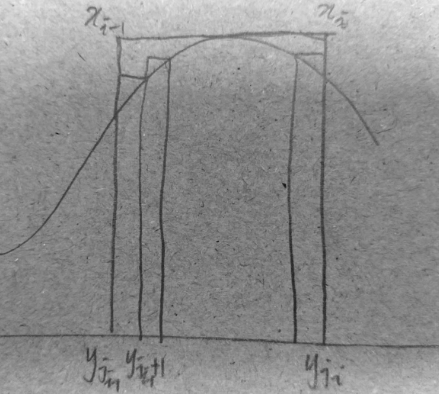
\includegraphics[width=0.5\linewidth]{images/RSintegral-partitions.png}
    \caption{Partitions}
\end{figure}

Continuing from
\[ \sup_{[x_{i-1},x_i]} f \ge \sup_{[y_{k-1},y_k]} f, \]
We then multiply by $\alpha(y_k)-\alpha(y_{k-1})$ on both sides and then take the sum from $k=j_{i-1}+1$ to $k=j_i$
:
The RHS corresponds to the (weighted) sum of the thin rectangles that you see in the above picture
:
The LHS is actually a telescoping sum, and the sum would be
\[ (\sup_{[x_{i-1},x_i]} f) \cdot [\alpha(y_{j_i})-\alpha(y_{j_{i-1}})] = (\sup_{[x_{i-1},x_i]} f) \cdot [\alpha(x_i)-\alpha(x_{i-1})] \]
Finally, we take the sum from $i=1$ to $i=n$ of the above inequality
LHS $\ge$ RHS (sorry I don't know of a better way to put it)
We then obtain $U(P,f,\alpha)\ge U(P^\prime,f,\alpha)$

(On the LHS we're collecting all the rectangles for the upper sum wrt $P$, but on the RHS we're collecting up collections of upper rectangles to obtain the entire collective of upper rectangles for the upper sum wrt $P^\prime$)
:
Lower sum is similar
:
Now, a lemma used to prove 6.5
Given any two partitions $P_1$ and $P_2$, we have
\[ L(P_1,f,\alpha)\le U(P_2,f,\alpha) \]
So a lower sum will always be no larger than any other upper sum
:
So this includes the cases where we have the most refined of $P_1$'s and $P_2$'s, with no information regarding the partition points whatsoever
To be honest, the result seems to be both intuitive and unclear at the same time

The key here is to use common refinements as a link for both sums
The idea is stated in the proof of 6.5 and I don't think I need to elaborate further

What's nice here is that now we have two completely independent partitions $P_1$ and $P_2$, so by fixing one partition, say $P_2$, and taking the 'limit' over the other (here we take the supremum over all possible $P_1$) we then obtain an inequality between a Darboux integral and a Darboux sum (here it's the lower integral and an upper sum)

Since the Darboux integral is just a number, we can then safely take the 'limit' over the other partition to obtain the inequality in 6.5
\end{proof}

\begin{proposition}
\[ \lowerint_a^bf\dd{\alpha}=\upperint_a^bf\dd{\alpha}. \]
\end{proposition}

\begin{proof}

\end{proof}

Now we move on to integrability conditions for $f$. The first one looks a lot like the $\epsilon-N$ or $\epsilon-\delta$ definition of limits:

\begin{theorem}
$f\in R_\alpha[a,b]$ if and only if for each $\epsilon>0$, there exists some partition $P$ such that
\[ U(f,\alpha;P)-L(f,\alpha;P)<\epsilon. \]
\end{theorem}
%%%%%%%%%%%%%%%%%%%%

\begin{proof} \

($\implies$) Assume $f\in R_\alpha[a,b]$. By definition,
\[ \inf_PU(f,\alpha;P)=\int_a^bf\dd{\alpha}=\sup_PL(f,\alpha;P). \]
For every $\epsilon>0$, 

($\impliedby$) 
\end{proof}



%%%%%%%%%%%%%%%%%%%%%%%%%
% Darboux sums, Darboux integrals

\begin{example}[Dirichlet function]
The Dirichlet function is given by
\[ f(x)=\begin{cases}
1 & x\in\QQ \\
0 & x\notin\QQ
\end{cases} \]
We try to calculate the two on the interval $[0,1]$.

The Dirichlet function is pathological because for each subinterval $[x_{i-1},x_i]$, the supremum is always $1$ and the infimum is always $0$.

So no matter what partition we use, $U(f,P)$ is always $1$ whereas $L(f,P)$ is always $0$. This means that $U(f)=1$ and $L(f)=0$, so there are two different values for ``the integral of $f$''.

This is like the case where we try to find the limit of the Dirichlet function where $x$ is approaching any given real number $r$, there exists two sequences approaching $r$ whose image approaches two different values.
\end{example}

Now, a very important and fun case about the more general RS-integral, which we'll discuss next week (do try the exercise yourself first)

\begin{exercise}
The Heaviside step function $H$ is a real-valued function defined by the following:
\[ H(x)=\begin{cases}
0 & x<0 \\
1 & x\ge0
\end{cases} \]
For the purpose of this question we assume the convention $\infty\cdot0=0$.
\begin{enumerate}[label=(\alph*)]
\item Let $f$ be a real-valued function over $\RR$. Show that $f\in\RR_H [a,b]$ iff $f$ is continuous at $0$, and find the RS-integral $\int_{-\infty}^\infty f\dd{H}$.
\item Suppose that the definition for $H$ is changed for $x=0$, say $H(0)=\frac{1}{2}$. Show that the above result still holds.
\item Examine the RS-integral of $f$ over $\RR\setminus\{0\}$ wrt $H$, where $f$ is a real-valued function over $\RR\setminus\{0\}$ such that $\lim_{x\to0}f(x)=\infty$ or $-\infty$.
\end{enumerate}
(You may read up on more information regarding the Heaviside function, and the (in)famous Dirac delta function)
\end{exercise}




Now we've been talking a lot about upper and lower sums because they're arguably the simplest way to define integrals, in the sense that there's not a whole lot of things that we could go wrong here
By considering only upper and lower bound, we're essentially picking the most conservative route possible

It would be nice if we could just pick like one random point within each interval and consequently calculate the Riemann(-Stieltjes) sums

This method, of course, fails to be well defined for pathological functions like the Dirichlet function
On the other hand, by using upper and lower sums, we could give a persuasive explanation as to why the Dirichlet function is not Riemann integrable

However, instead of throwing this idea away, there's actually a way for us to make this into a strict definition

When we were talking about the sequential definition for limits of functions, we noted that there are certain scenarios where the limit cannot exist because there may be two distinct sequences may give different limit
Based on this observation, we then gave a reasonable condition as follows:
"$\lim_{x\to a} f(x)$ exists and is equal to $L$ iff for all sequences $x_n$ converging but not containing a, $f(x_n)$ converges to $L$"

Well here, it's actually the same kind of scenario
Given any partition $P$, we consider the Riemann sum $\sum f(\xi_i)\Delta x_i$ where $\xi_i$ is any point where $x_{i-1}\le\xi_i\le x_i$

For the Dirichlet function over $[0,1]$, given any partition P (here we may assume that the partition points are distinct), we will always be able to specifically pick $\xi_i,\eta_i\in[x_{i-1},x_i]$ such that $\xi_i$ is rational but $\eta_i$ is irrational

Then $\sum f(\xi_i)\Delta x_i=1$ but $\sum f(\eta_i)\Delta x_i=0$

Now be very mindful that this alone cannot be evidence that f is non-integrable
The key is that this somehow occured for all partitions P, no matter how refined they are; for every single partition P, there exists two sets of 'representing points' $\xi_i,\eta_i$ such that the two Riemann sums are constantly far apart (1 and 0 in this case)

Let $\epsilon_0=1$, then this ultimately translates to the following:
The Dirichlet function cannot be Riemann integrable because
There exists some $\epsilon_0>0$, such that for any given partition $P$, there exists two sets of representing points $\xi_i,\eta_i$ such that their corresponding Riemann sums satisfy that
\[ |\sum f(\xi_i)\Delta x_i - \sum f(\eta_i)\Delta x_i|\ge\epsilon_0. \]

Now if we always pick the representatives such that $\xi_i>\eta_i$ then we can neglect the absolute value

So now, let's take the converse
A function $f$ is said to be RS-integrable if
For every $\epsilon>0$,
There exists a partition P, such that
For any two sets of representing points $\xi_i,\eta_i$,
Their corresponding Riemann sums satisfy that
\[ \sum[f(\xi_i)-f(\eta_i)]\Delta x_i<\epsilon \]
(The last one should be $\Delta \alpha_i$ for RS-integrals, not $\Delta x_i$)

Unfortunately this is still not quite the correct definition according to Apostol, but we're pretty close
The problem with this definition is that it is too weak if we're considering general $\alpha$ of bounded variation; if we were only talking about monotonically increasing $\alpha$ then this will actually be an equivalent definition

The official definition for the RS-integral wrt $\alpha$ of bounded variation is as follows:
\begin{definition}
For every $\epsilon>0$, there exists a partition $P$, such that
[For any refinement $P^\prime$ of P, and]
For any two sets of representing points $\xi_i,\eta_i$ [of $P^\prime$], their corresponding Riemann sums satisfy that
\[ \sum[f(\xi_i)-f(\eta_i)]\Delta x_i<\epsilon. \]
\end{definition}

Now this definition is what mathematicians would refer to as a 'Cauchy' definition, since it defines a notion by comparing a pair of arbitrary values that are similar to one another, and if they agree in some sense then we say that that something satisfies some property.

The integral is then obtained as follows: If $f$ were to satisfy the above Cauchy definition, then we may pick an arbitrary sequence of refinements
\[ P_1 \subset P_2 \subset P_3 \subset ...; \]
and for each partition we pick a set of representatives to obtain a sequence RS-sum
$I_1, I_2, I_3, ...$
:
This sequence will be a Cauchy sequence of real numbers, and so will converge to a specific value $I$ which we consider to be RS-integral of f
:
Now the reason why Apostol needed to strengthen the definition is that, otherwise this value $I$ may not be unique
:
So if you look at the statement you see in 6.7(b)(c), then they correspond to the Cauchy definition and the 'value-based' definition respectively
For monotonically increasing $\alpha$, it is much easier to discuss them using upper and lower sums
So your exercise today will be to read the statements and proofs in Theorem 6.7

\begin{theorem}
$f\in R_\alpha[a,b]$, $m\le f\le M$, and $\phi$ is uniformly continuous on $[m,M]$, then
\[ \phi\circ f\in R_\alpha[a,b]. \]
\end{theorem}

\begin{proof}
Choose $\epsilon>0$. Since $\phi$ is uniformly continuous on $[m,M]$, there exists $\delta>0$ such that $\delta<\epsilon$ and $|\phi(s)-\phi(t)|$
\end{proof}

\section{Properties of the Integral}
\begin{theorem} \
\begin{enumerate}[label=(\arabic*)]
\item If $f_1,f_2\in R_\alpha[a,b]$, then 
\[ f_1+f_2\in R_\alpha[a,b]; \]
$cf\in R_\alpha[a,b]$ for every $c\in\RR$, and
\[ \int_a^b(f_1+f_2)\dd{\alpha}=\int_a^bf_1\dd{\alpha}+\int_a^bf_2\dd{\alpha}, \]
\[ \int_a^b(cf)\dd{\alpha}=c\int_a^bf\dd{\alpha}. \]

\item If $f_1,f_2\in R_\alpha[a,b]$ and $f_1\le f_2$, then
\[ \int_a^bf_1\dd{\alpha}\le\int_a^bf_2\dd{\alpha}. \]

\item If $f\in R_\alpha[a,b]$ and $c\in[a,b]$, then $f\in R_\alpha[a,c]$ and $f\in R_\alpha[c,b]$, and
\[ \int_a^bf\dd{\alpha}=\int_a^c\dd{\alpha}+\int_c^b\dd{\alpha}. \]

\item If $f\in R_\alpha[a,b]$ and $|f|\le M$, then
\[ \absolute{\int_a^bf\dd{\alpha}}\le M\sqbrac{\alpha(b)-\alpha(a)}. \]

\item If $f\in R_{\alpha_1}[a,b]$ and $f\in R_{\alpha_2}[a,b]$, then $f\in R_{\alpha_1+\alpha_2}[a,b]$ and
\[ \int_a^bf\dd{(\alpha_1+\alpha_2)}=\int_a^bf\dd{\alpha_1}+\int_a^bf\dd{\alpha_2}; \]
if $f\in R_\alpha[a,b]$ and $c$ is a positive constant, then $f\in R_{c\alpha}[a,b]$ and
\[ \int_a^bf\dd{(c\alpha)}=c\int_a^bf\dd{\alpha}. \]

\item If $f\in R_\alpha[a,b]$ and $g\in R_\alpha[a,b]$, then $fg\in R_\alpha[a,b]$.
\end{enumerate}
\end{theorem}

\begin{proof} \
\begin{enumerate}[label=(\arabic*)]
\item If $f=f_1+f_2$ and $P$ is any partition of $[a,b]$, we have
\begin{align*}
L(f_1,\alpha;P)+L(f_2,\alpha;P)&\le L(f,\alpha;P)\\
&\le U(f,\alpha;P)\\
&\le U(f_1,\alpha;P)+U(f_2,\alpha;P).
\end{align*}

If $f_1\in R_\alpha[a,b]$ and $f_2\in R_\alpha[a,b]$, let $\epsilon>0$ be given. There are partitions $P_1$ and $P_2$ such that


\item 
\item 
\item 
\item 
\item 
\end{enumerate}
\end{proof}

\begin{theorem}[Triangle inequality]
$f\in R_\alpha[a,b]$, then $|f|\in R_\alpha[a,b]$,
\[ \absolute{\int_a^bf\dd{\alpha}}\le\int_a^b|f|\dd{\alpha}. \]
\end{theorem}

\begin{proof}

\end{proof}

6.14 6.15
Heaviside step function

6.16 corollary
for intinite sum, need $\sum c_n$ to converge
(23) comparison test

6.17 integration by substitution
\begin{theorem}
$\alpha$ increasing, $\alpha^\prime\in R[a,b]$, $f$ bounded on $[a,b]$, then
\[ f\in R_\alpha[a,b]\iff f\alpha^\prime\in R[a,b]. \]
\end{theorem}

6.19 change of variables

\section{Fundamental Theorem of Calculus}
6.20 6.21

\begin{theorem}

\end{theorem}

6.22 integration by parts

\chapter{Sequence and Series of Functions}
\section{Uniform Convergence}
\begin{definition}
Suppose $\{f_n\}$, $n=1,2,3,\dots$ is a sequence of functions defined on a set $E$, and suppose that the sequence of numbers $\{f_n(x)\}$ converges for every $x\in E$. We can then define a function $f$ by
\[ f(x)=\lim_{n\to\infty}f_n(x). \]
We say that $\{f_n\}$ \vocab{converges pointwise} to $f$ on $E$, denoted by $f_n\to f$.

Similarly, if $\sum f_n(x)$ converges for every $x\in E$, and if we define
\[ f(x)=\sum_{n=1}^\infty f_n(x) \]
the function $f$ is called the \vocab{sum of the series} $\sum f_n$.
\end{definition}
pointwise convergence

\begin{definition}
Assume $\{f_n\}$ is a sequence of functions defined over a set $X$ and $f$ is also a function defined over $X$. We say $\{f_n\}$ \vocab{uniformly converges} to $f$ over $X$, if for any $\epsilon>0$, there exists $N>0$ (which is independent of $x$) so that for any $x\in X$,
\[ |f_n(x)-f(x)|<\epsilon. \]
\end{definition}

\begin{notation}
We denote this uniform convergence over $X$ by $f_n\rightrightarrows f$.
\end{notation}

\section{Uniform Convergence and Continuity}

\section{Uniform Convergence and Integration}
\begin{theorem}
Assume $\{f_n\}$ is a sequence of functions defined over $[a,b]$ and each $f_n\in R_\alpha[a,b]$. If $f_n\to f$, then $f\in R_\alpha[a,b]$, and
\[ \lim_{n\to\infty}\int_a^bf_n\dd{\alpha}=\int_a^bf\dd{\alpha}. \]
\end{theorem}

\begin{proof}
Define
\end{proof}

\begin{corollary}
Assume $a_n\in R_\alpha[a,b]$ and
\[ f(x)\coloneqq\sum_{n=0}^\infty a_n(x) \]
converges uniformly. Then it follows
\[ \int_a^bf\dd{\alpha}=\sum_{n=0}^\infty a_n\dd{\alpha}. \]
\end{corollary}

\begin{proof}
Consider the sequence of partial sums 
\[ f_n(x)\coloneqq\sum_{k=0}^na_k(x), \quad n=0,1,\dots \]
It follows $f_n\in R_\alpha[a,b]$ and $f_n\rightrightarrows f$. Apply above theorem to $\{f_n\}$ and the conclusion follows.
\end{proof}

\section{Uniform Convergence and Differentiation}
\begin{theorem}
Assume $\{f_n\}$ is a sequence of functions defined over $[a,b]$ and differentiable. If $\{f_n^\prime\}$ uniformly converges on $[a,b]$ and $\{f_n\}$ converges at some point $x_0\in[a,b]$, then $\{f_n\}$ uniformly converges on $[a,b]$ to some function $f$. Moreover, $f$ is differentiable and
\[ f^\prime(x)=\lim_{n\to\infty}f_n^\prime(x) \]
for any $x\in[a,b]$.
\end{theorem}

\begin{proof}

\end{proof}

\section{Stone--Weierstrass Approximation Theorem}


\chapter{Some Special Functions}
\section{Power Series}
We derive some properties of functions represented by \vocab{power series}, i.e. functions of the form
\[ f(x)=\sum_{n=0}^\infty c_nx^n \]
or, more generally,
\[ f(x)=\sum_{n=0}^\infty c_n(x-a)^n. \]
These are called \vocab{analytic functions}.

If $f(x)$ converges for $|x-a|<R$, $f$ is said to be expanded in a power series about the point $x=a$. For convenience, we take $a=0$ without loss of generality. We call $R$ the \vocab{radius of convergence}.

\begin{theorem}
Suppose the series 
\[ \sum_{n=0}^\infty c_nx^n \]
converges for $x\in(-R,R)$. Then
\begin{enumerate}[label=(\arabic*)]
\item $\sum_{n=0}^\infty c_nx^n$ converges uniformly on the closed interval $[-R,R]$;
\item $f(x)$ is continuous and differentiable on $(-R,R)$, and 
\[ f^\prime(x)=\sum_{n=1}^\infty nc_nx^{n-1}. \]
\end{enumerate}
\end{theorem}

\begin{proof} \
\begin{enumerate}[label=(\roman*)]
\item 
\item 
\end{enumerate}
\end{proof}
%\part{Topology}
\chapter{$n$-dimensional Euclidean space}
\section{Topology in Euclidean Space}
\begin{itemize}
\item Basic constructions
\item 
The \textbf{interior} of a set $A$, denoted by $A^\circ$, is the set of all interior points in $A$.

A set $A\subset\RR^n$ is called an \textbf{open set} if $A^\circ=A$, i.e. all points in $A$ are interior points.

\item Limit points, closure and closed sets

An element $x\in A$ is called a limit point of $A$ if $B_0(x,\epsilon)\cap A\neq\emptyset$ for all $\epsilon>0$.

The induced set of a set, denoted by $A^\prime$, is the set of all limit points of $A$.

The closure of a set $A$, denoted by $\bar{A}$, is the union set $A\cup A^\prime$.

A set $A\subset RR^n$ is called a closed set if $\bar{A}=A$, i.e. all limit points of $A$ are contained in $A$

\item Further topological constructions of points

An element $x\in A$ is called an isolated point of $A$ if it is not a limit point of $A$.

The boundary of a set $A$, denoted by $\partial A$, is the set difference $\bar{A}\setminus A^\circ$.

An element $x\in\RR^n$ is called a boundary point of $A$ if it is in $\partial A$.

An element $x\in\RR^n$ is called an exterior point of $A$ if it is an interior point of $A^c$.

\item Further topological constructions of sets

A set $A\subset\RR^n$ is compact if it is a bounded closed set.

A subset $B\subset A$ is called a dense subset of $A$ if $\bar{B}=A$.

A set $A\subset\RR^n$ is nowhere dense its closure has no interior, i.e. $(\bar{A})^\circ=\emptyset$.
\end{itemize}

In general topology, these are the axioms used to define open and closed sets. At the moment we only consider them to be certain properties regarding open and closed sets in $\RR^n$.
\begin{enumerate}[label=\textbf{P\arabic*}]
\item $A$ is open if and only if $A^c$ is closed.

\begin{proof}
\textbf{Forward direction}:
Let $A$ be open, we consider the punctured balls of $x \notin A$ (if $x \notin A$, we consider the punctured balls centered at $x$).

Our goal is to show that $B_0(x,r)$ always intersects with $A^c$

So suppose otherwise that $B_0(x,\epsilon)$ is a subset of A for some $\epsilon>0$

Ah no sorry, we consider x not in $A^c$

The thing is we want to show that $A^c$ is closed, i.e. all limit points of $A^c$ are in $A^c$

So suppose otherwise that $x$ is a limit point of $A^c$ that is not in $A^c$

$x$ is a limit point of $A^c$, hence for all $\epsilon>0$, $B_0(x,\epsilon)$ always intersects with $A^c$

This is equivalent to saying that $B_0(x,\epsilon)$ is never a subset of $(A^c)^c=A$

However, $x$ is not in $x \notin A^c$, so $x \in A$.

But if A is open, then there exists $\epsilon>0$ such that $B(x,\epsilon)$ is a subset of $A$, a contradiction

\textbf{Backward direction}: Let $A^c$ be closed. Suppose otherwise that $A$ is not open, i.e. there is a point $x\in A$ such that $B(x,\epsilon)$ is never a subset of $A$; that is to say, $B(x,\epsilon)$ always intersects with $A^c$

Since $x \in A$, then $B(x,\epsilon) \cap A^c = B_0(x,\epsilon) \cap A^c$

But this means that $B_0(x,\epsilon) \cap A^c$ is never empty, hence $x$ is a limit point of $A^c$.

However, $x \in A$, contradictory to $A^c$ being closed and thus should contain all of its limit points
\end{proof}

\item An arbitrary union of open sets is open; a finite intersection of open sets is open.

\begin{proof}
Let $A$ be an arbitrary union of open sets $\{U_i\}_{i \in I}$.

Then for any $x \in A$, suppose that $x \in U_i$, then since $U_i$ is open we can pick $B(x,\epsilon)$ subset of $U_i$ subset of $A$

On the other hand, let $U$ and $V$ be open sets and let $x \in U \cap V$. 
Since $U$ and $V$ are open, we can pick $\epsilon_1$ and $\epsilon_2$ such that $B(x,\epsilon_1)$ is in $U$ whereas $B(x,\epsilon_2)$ is in $V$. 
Then we simply pick $\epsilon=\min\{\epsilon_1,\epsilon_2\}$ so that $B(x,\epsilon)$ is in $U \cap V$.
\end{proof}

\item An arbitrary intersection of closed sets is closed; a finite union of closed sets is closed.

\begin{proof}
This follows from de Morgan's Law on P1 and P2.
\end{proof}
\end{enumerate}

\begin{prbm}\label{sizes}
Compare the sizes of the following pairs of sets, i.e. determine if they are equal, or if one set may be a subset of the other.
\begin{enumerate}
\item $(A\cup B)^\circ$, $A^\circ\cup B^\circ$
\item $(A\cap B)^\circ$, $A^\circ\cap B^\circ$
\item \label{size} $\overline{A\cup B}$, $\bar{A}\cup\bar{B}$
\item $\overline{A\cap B}$, $\bar{A}\cap\bar{B}$
\end{enumerate}
\end{prbm}

\begin{proof} \
\begin{enumerate}
\item $(A\cup B)^\circ$ may be bigger

In $\RR$ we consider the intervals $A=(-1,0]$ and $B=[0,1)$, then
\[ A^\circ\cup B^\circ=(-1,0)\cup(0,1), \quad (A\cup B)^\circ=(-1,1) \]

For $x \in A^\circ \cup B^\circ$, we have either $x \in A^\circ$ or $x \in B^\circ$, so there is some ball centered at $x$ that is contained in either $A$ or $B$ and thus must be contained in $A\cup B$ as well.

\item Equal

If $x \in (A\cap B)^\circ$, then there exists a ball $U$ centered at $x$ such that $U$ is in both $A$ and $B$, so $x$ is in both $A^\circ$ and $B^\circ$.

On the other hand, $A^\circ\cap B^\circ$ is a subset of $A\cap B$; taking the interior of both sides, then since the intersection between two open sets is open we find that $A^\circ\cap B^\circ$ is a subset of $(A\cap B)^\circ$.

\item Equal

\item $\bar{A}\cap\bar{B}$ may be bigger
\end{enumerate}
\end{proof}

\begin{prbm}
Prove that the set of exterior points, $(A^c)^\circ$ is the same as $(\bar{A})^c$.
\end{prbm}

\begin{proof}
\begin{align*}
x \in (A^c)^\circ 
&\iff \exists \epsilon>0 \text{ such that } B(x,\epsilon) \subset A^c \\
&\iff B(x,\epsilon) \cap A = \emptyset \\
&\iff x \notin A \text{ and } B_0(x,\epsilon) \cap A=\emptyset \\
&\iff x \notin A \cup A^\prime = \bar A \\
&\iff x \in (\bar A^c)
\end{align*}
\end{proof}

\begin{prbm}
Regarding alternative descriptions:
\begin{enumerate}
\item $A$ is a neighbourhood of x if and only if there exists an open set U such that x is in U, U is subset of A (trivial except you'll actually need to prove that balls are open sets).
\item If $x$ is a limit point of $A$, then in fact for any $\epsilon>0$, $B(x,\epsilon)$ contains infinitely many elements of $A$ (you don't need to mention the punctured ball here because of obvious reasons; converse is trivial but a good and intuitive description).
\item $x$ is a boundary point of $A$ if and only if for all $\epsilon>0$, $B(x,\epsilon)$ intersects with both $A$ and $A^c$.
\end{enumerate}
\end{prbm}

\begin{proof} \
\begin{enumerate}
\item We show that $B(x,\epsilon)$ is open:

$\forall y \in B(x,\epsilon)$, 
\[ |y-x|<\epsilon \]

$\forall z \in B(y,\epsilon-|y-x|)$, 
\[ |z-x|\le|z-y|+|y-x|<\epsilon-|y-x|+|y-x|=\epsilon \]

$\therefore\:B(y,\epsilon-|y-x|) \subset B(x,\epsilon)$

\item We construct a sequence $\{x_n\}$ recursively as follows:
\begin{itemize}
\item Pick $x_1 \in B_0(x,\epsilon) \cap A$
\item Pick $x_{n+1} \in B_0(x,|x_n-x|) \cap A$
\end{itemize}
It is easy to see that the balls above are getting smaller so all $x_n$ are both mutually distinct and all contained in $B(x,\epsilon)$.

\item $x$ is a boundary point if and only if $x \in \bar{A} \setminus A^\circ$

\textbf{Forward direction}: 

We consider two cases
\begin{itemize}
\item $x \in A$, then all $B(x,\epsilon)$ intersects with $A$ at $x$, but since x is not in $A^\circ$ they must always intersect with $A^c$ as well.
\item $x \notin A$, then all $B(x,\epsilon)$ intersect with $A^c$ at $x$, but since $x \in \bar{A}$, $x$ is a limit point of $A$ and thus $B(x,\epsilon)$ always intersects with $A$.
\end{itemize}

\textbf{Backward direction}:

We consider two cases
\begin{itemize}
\item $x \in A$, then since $B(x,\epsilon)$ always intersects with $A^c$, $x$ cannot be in $A^\circ$.
\item $x \notin A$, then since $B(x,\epsilon)$ always intersects with $A$, $x$ must be in $\bar{A}$.
\end{itemize}

In fact we can describe the closure without referring to punctured balls and induced sets:
$x \in \bar{A}$ if and only if $B(x,\epsilon)$ always intersects with $A$

Also as a side note, $A\circ\cup \partial A\cup (A^c)\circ=\RR^n$
\end{enumerate}
\end{proof}

\begin{prbm}
Regarding closures (The following properties are relatively nontrivial compared to its 'open-set' counterparts):
\begin{enumerate}[label=(\alph*)]
\item $A^\prime$ is closed.
\item $\bar{A}$ is closed, i.e. bar(barA)=barA
\end{enumerate}
\end{prbm}

\begin{proof} \
\begin{enumerate}[label=(\alph*)]
\item In order to show that $A^\prime$ is closed, we need to show that if $x$ is a limit point of $A^\prime$, then $x\in A^\prime$, i.e. $x$ is a limit point of $A$.

So we need to show that limit points of $A^\prime$ are always limit points of $A$: 
Let $x$ be a limit point of $A^\prime$, then for all $\epsilon>0$, $B_0(x,\epsilon/2)$ intersects with $A^\prime$ and we may pick $y \in B_0(x,\epsilon/2)\cap A^\prime$

Now here's the tricky part
Since $y \in A^\prime$, y is a limit point of $A$, hence $B_0(y,|y-x|)$ intersects with $A$ and thus we may pick $z \in B_0(y,|y-x|)\cap A$.

We show that $z \in B_0(x,\epsilon)$:
\[ |z-x|\le|z-y|+|y-x|<2|y-x|<\epsilon, \]
hence $z \in B(x,\epsilon)$.
\[ |z-y|<|x-y|, \]
hence $z \neq x$

$\therefore\:z \in B_0(x,\epsilon)$

\item As for (b), it is just (a) and \cref{sizes} \cref{size}.
\end{enumerate}
\end{proof}

For homework, you'll work out some properties regarding dense sets

1. $A$ is a dense set in $X$ if and only if $A$ intersects with all open sets in $X$.
2. If $A$ is dense in $X$ and $B$ is dense in $A$, then $B$ is dense in $X$
3. If $A$ and $B$ are dense in $X$ where $A$ is open, then $A\cap B$ is dense in $X$

\section{Important Theorems}
\begin{thrm}{Cantor's Intersection Theorem}{}
Given a decreasing sequence of compact sets $A_1\supset A_2 \supset \cdots$, there exists a point $x\in\RR^n$ such that $x$ belongs to all $A_i$. In other words, $\bigcap_{i=1}^\infty A_i\neq\emptyset$. Moreover, if for all $i\in\NN$ we have $\diam A_{i+1}\le c\cdot\diam A_k$ for some constant $c<1$, then such a point must be unique, i.e. $\bigcap_{i=1}^\infty A_k=\{x\}$ for some $x\in\RR^n$.
\end{thrm}

\begin{thrm}{Heine--Borel Theorem}{}
A set $A\subset\RR^n$ is compact if and only if every open covering has a finite subcover, i.e. for any family of open sets $\mathscr{U}=\{U_i\}_{i\in I}$ satisfying $A\subset\bigcup_{i\in I}U_i$, there exists $\{U_1,\dots,U_n\}\subset\mathscr{U}$ such that $A\subset\bigcup_{i=1}^n U_i$.
\end{thrm}

\begin{thrm}{Bolzano--Weierstrass Theorem}{}
Infinite bounded sets in $\RR^n$ must contain limit points.
\end{thrm}

We will follow a very specific sequence of steps to prove these three theorems:
\begin{enumerate}[label=(\alph*)]
\item Cantor Intersection for $n=1$
\item Bolzano--Weierstrass for $n=1$
\item Bolzano--Weierstrass for general $n$
\item Cantor Intersection for general $n$
\item Heine--Borel for general $n$
\end{enumerate}

\begin{proof} \
\begin{enumerate}[label=(\alph*)]
\item Suppose that there is a decreasing sequence of compact sets $A_1, A_2, \dots$ in the real numbers

Since $A_k$ are bounded, we may let $a_k=\inf A_k$
Also since $A_k$ are closed, $a_k \in A_k$

Note that since $A_k$ is a decreasing sequence of sets we have $a_1\le a_2\le\dots$

Also, whenever we have $n>k$, we have $a_n \in A_n$, but $A_n \subset A_k$ and thus $a_n \in A_k$.

Let $b_1=\sup A_1$, then $a_k \in A_1$ and thus $a_k\le b_1$ for all $k$.

This tells us that the sequence $\{a_k\}$ is bounded above, and thus we may let $a=\sup a_k$.

Our goal is to show that the number $a$ appears in all $A_k$, thus showing that the entire intersection $\bigcap A_k$ contains $a$ and thus must be non-empty.

Now we split this in two cases, which asks whether a is simply made from isolated points, or if it is actually some nontrivial point obtained from the boundaries of $A_k$

\textbf{Case 1:} $a_k=a$ for some $k$
In this case we see that $a_k\le a_n\le a$ for all $n>k$ and thus $a_n=a$ in this case, therefore a is an element in $A_n$ for all $n$

In this case you can imagine that there is a possibility where a is an isolated minimum point of $A_n$ which stays there forever in the decreasing sequence of sets

\textbf{Case 2:} $a_k<a$ for all $k$; in this case we see that $a$ is the limit point of the increasing sequence $\{a_k\}$

Exercise 1: Show that $a$ is a limit point of each $A_k$.

Note that $a_n$ is in $A_k$ for each $n>k$, and since $a=\sup\{a_k\}$ where $a_k$ is increasing, we can actually show that a is a limit point of $\{a_n \mid n \le k\}$:
For every $\epsilon>0$, we pick $n_0$ such that $0 < a-a_{n_0} < \epsilon$
Pick $n\prime > \max\{k,n_0\}$, then $a_{n^\prime} \ge a_{n_0}$ and so
\[ 0<a-a_n\prime \le a_{n_0} < \epsilon \]
This shows that there exists $a_n^\prime$ in $B_0(a,\epsilon) \cap \{a_n \mid n>k\}$ for all $\epsilon$, and so $a$ is a limit point of $\{a_n \mid n>k\}$.

Now since $\{a_n|n \ge k\}$ is a subset of $A_k$ we also see that a is a limit point of $A_k$
Finally, since $A_k$ is closed, we conclude that $a$ is in $A_k$ for all $k$, and we are done

Wait hold on, I forgot about the second part

Now we consider a decreasing sequence of compact sets $A_1, A_2, \dots$ such that $\diam A_{k+1} \le c \diam A_k$ for $c<1$.

Suppose otherwise that there exists $x, y$ in $\bigcap A_k$

You can imagine that this will form a fixed distance between two points, and thus there is a constant positive lower bound for the diameters:
\[ \diam A_k \ge |x-y| > 0 \forall k \]

But this cannot be true because $\diam A_{k+1} \le c \diam A_k$ and so the diameter is controlled by a decreasing geometric sequence:
\[ \diam A_{k+1} \le c^k \diam A_1 \]

So we can simply pick a natural number $k$ such that
\[ k > \log_c \frac{|x-y|}{\diam A_1} \]

\item We consider an infinite bounded set $A$ in the real numbers. Since $A$ is bounded, we can pick a closed interval $[a_1,b_1]$ containing $A$.

We then perform a series of binary cuts: Consider the two halves of $[a_1,b_1]$. We know that at least one of these two must contain infinitely many elements in $A$, otherwise $A$ cannot be infinite. We pick this half of the interval and denote it by $[a_2,b_2]$. We continue this to pick a decreasing sequence of closed intervals $[a_n,b_n]$.

Now $\diam [a_{n+1},b_{n+1}] = \frac{1}{2} \diam [a_n,b_n]$, so by the Cantor Intersection Theorem, there exists a unique real number $c$ in the intersection $\bigcap[a_n,b_n]$.

We show that this $c$ is in fact a limit point of $A$.

For any $\epsilon>0$, we need to show that $B_0(c,\epsilon) \cap A \neq \emptyset$, i.e. we need to find an element $x \neq c$ in $A$ that is less than $\epsilon$ apart from $c$.

We then realize that we can simply exploit the decreasing sequence $[a_n,b_n]$
Since $\diam [a_n,b_n]$ is controlled by a decreasing sequence:
\[ \diam [a_{n+1},b_{n+1}] \le 1/2^n \diam [a_1,b_1] \]
We take a sufficiently large n so that $b_n-a_n<\epsilon$
Since $c$ is in $[a_n,b_n]$, for all $x$ in $[a_n,b_n]$ we have $|x-c|\le b_n-a_n<\epsilon$ and therefore $[a_n,b_n]$ is within $B(c,\epsilon)$.

Here's the funny part: $[a_n,b_n]$ contains infinitely many elements of $A$, so it must contain at least one element in A that is not $c$.

Therefore this element $x \neq c$ is in $B_0(c,\epsilon)$.

\item Now we have an infinte bounded set $A$ in $\RR^n$

The idea here is to consecutively come up with better and better sequences of points in $A$. We denote $x_i$ to be the $i$-th coordinate in $\RR^n$.

Our first wish is to pick some elements in $A$ so that they sort of converge at $x_1$.

Because such considerations of 'restricting to a single coordinate' is important here, we define the projection map to the $i$-th coordinate by
\[ f_i(x_1,\dots,x_n)=x_i \]

So, we look at $f_i(A)$ and try to apply BW for the case where $n=1$.

However, the problem is that $f_i(A)$ need not be infinite. For example, the set $\{(0,0),(0,1),(0,2),\dots\}$ projected onto the first coordinate is simply $\{0\}$.

This forces us to consider two cases

Exercise 2: Show that $f_i(A)$ is bounded
This is simple
1. $f_1(A)$ is infinite, then we can apply BW(n=1) to find a real number $c_1$ which is a limit point in $f_1(A)$

Here we can construct a sequence of points 
\[ \{x^{(1),1},x^{(1),2},...\} \]
so that their first coordinates satisfy
\[ |x^{(1),n}_1-c_1| < 1/n \]
for all natural number n
(I know this notation is cumbersome but the problem is that we need multiple sequences for this proof)

2. $f_1(A)$ is finite, then by the Pigeonhole Principle there exists a real number $c_1$ such that its preimage $f_1^{-1}(c_1)$ in $A$ is infinite

In this case we can randomly pick a sequence $\{x^{(1),1},x^{(1),2},\dots\}$ in $A$ so that their first coordinate is equal to $c_1$

I forgot to mention something that is implied, but we actually do have the need to emphasize that the sequence $\{x^{(1),1},x^{(1),2},\dots\}$ can be chosen to contain mutually distinct entries

Now that we have a sequence that behaves nice on the first coordinate, we may then move on to the second coordinate

Let $A_1=\{x^{(1),1},x^{(1),2},\dots\}$
We again consider $f_2(A_1)$ in two cases, infinite or finite

In any case, we are able to find a subsequence $\{x^{(2),1},x^{(2),2},\dots\}$, where
$x^{(2),k}=x^{(1),n_k}$ for some strictly increasing sequence of natural numbers $n_k$

So that, for the limit point/point with infinite preimage $c_2$, this sequence satisfies
\[ |f_2(x^{(2),n})-c_2| < \frac{1}{n} \]
Note that the property we have for the second case (we in fact have $f_2(x^{(2),n})=c_2$) is just a better version of this.

Now, take note that picking this subsequence does no harm whatsoever towards the first coordinate (if anything it would turn out to be better) since
\[ |f_1(x^{(2),k})-c_1| = |f_1(x^{(1),n_k}-c_1| < \frac{1}{n_k} \le \frac{1}{k} \]
($n_1<\dots<n_k$ is a strictly increasing sequence of natural numbers so $n_k \ge k$)

This continues on until we obtain a sequence of points $\{x^{(n),1},x^{(n),2},\dots\}$ in $A$ so that
\[ |f_i(x^{(n),k}-c_i|<\frac{1}{k} \quad \forall i,k \]

As we can see, the point $c=(c_1,\dots,c_n)$ is in fact a limit point of $A$ as we can always choose a big enough $k$ so that $x^{(n),k}$ is in $B(c,\epsilon) \cap A$.

Since $\{x^{(n),k}\}$ was always chosen to be a sequence of distinct entries, there is no danger for this sequence to always be c, and so c must be a limit point of $A$.

\item We may now return to the general case of Cantor.

Suppose that there is a sequence of decreasing compact sets $A_1,A_2,\dots$ in $\RR^n$. 
Note that every point is contained in $A_1$, so boundedness will never be an issue here.

Since $A_k$ are all nonempty, we can simply pick any element $a_k$ from $A_k$.

For the uncannily specific case that there are only finitely many $\{a_k\}$ chosen, we simply note that, again by Pigeonhole Principle, one of the $a_k$ appears infinitely often; thus for each $A_n$ we simply pick $n_k>n$ so that $A_{n_k}$ contains $a_k$, then $a_k$ is in $A_{n_k}$ which is a subset of $A_n$.

Otherwise, we can then note that $\{a_k\}$ is an infinite bounded set of points, so there must exist a limit point a of $\{a_k\}$.

We can now see that $a$ is always an element of $A_k$:
Using the same technique as Exercise 1, we see that a is a limit point of $\{a_n \mid n>k\}$ and so is a limit point of $A_k$, therefore a is in $A_k$ as $A_k$ is closed.

This proves the first part of the statement
The second part is completely identical to the second part of the $n=1$ case so we don't need to waste our time there either

\item We now consider a compact set A with some open covering $\mathscr{U}$.

This theorem is proved by contradiction: 
Suppose otherwise that set $A$ cannot be covered by any finite collection of open sets in $\mathscr{U}$

Since $A$ is compact, we may enclose it in a closed cube $Q_1$ (whose edges are parallel to the axes)

Now, for each step, we partition $Q$ into $2^n$ cubes by cutting it in half from each direction.

Then, starting from $Q_1$, there must exist one of these smaller cubes, denoted by $Q_2$, such that $A \cap Q_2$ cannot be covered by a finite collection of open sets in $\mathscr{U}$. 
Otherwise, if each $A \cap Q$ has a finite cover, then we simply collect all of these open sets together to form a finite cover of $A$, which violates our assumption.

We continue on to partition $Q_n$ and pick $Q_{n+1}$ so that $A_{n+1}$ has no finite cover (denote $A_n = A \cap Q_n$).

Note that $A$ and $Q_n$ are both compact, so $A_n$ is compact
Also we see that there is a decreasing sequence $A_1,A_2,\dots$
(we can't exactly obtain a relation between $\diam A_n$ and $\diam A_{n+1}$ here)

By Cantor Intersection Theorem we can always find a point $x$ in $A$ located in the intersection $\bigcap A_k$.

Now, since $\mathscr{U}$ is an open covering of $A$, there exists an open set $U$ in $\mathscr{U}$ such that $x\in U$.

The final key step is to exploit the sequence of decreasing cubes $Q_n$. So even though there isn't a clear cut way to control the sizes of $\diam A_n$, we do in fact have the property that $\diam Q_{n+1} = \frac{1}{2^n} \diam Q_1$.

Therefore, by picking a sufficiently large $n$, we can obtain $Q_n$ that is contained in $U$.

But this is a contradiction. 
This is because we've specifically chosen the sequence $A_n$ to be sets that do not possess any finite cover $\{U_1,...,U_n\}$ in $\mathscr{U}$. But here $A_n$ simply would have a one-element cover $\{U\}$.

This completes our proof.
\end{enumerate}
\end{proof}
\pagebreak

\section{Structures}\todo{to incorporate into other sections}
Let $X$ be a metric space. All points and sets mentioned below are understood to be elements and subsets of $X$ respectively.
\begin{itemize}

$A$ is \emph{open} if every point of $A$ is an interior point of $A$, i.e. $A^\circ=A$.

\item A point $x\in A$ is a \emph{limit point} of $A$ if every neighborhood of $x$ contains a point $y \neq x$ such that $y \in A$.

This means $B_0(x,\epsilon) \cap A \neq \emptyset$ for all $\epsilon>0$.

The \emph{induced set} of $A$, denoted by $A^\prime$, is the set of all limit points of $A$.

The \emph{closure} of $A$, denoted by $\bar{A}$, is the union set $A\cup A^\prime$. $A$ is \emph{closed} if all limit points of $A$ are contained in $A$, i.e. $\bar{A}=A$.

\item A point $x \in A$ is an \emph{isolated point} of $A$ if $x$ is not a limit point of $A$.

\item The \emph{boundary} of a set $A$, denoted by $\partial A$, is the set difference $\bar{A}\setminus A^\circ$.

A point $x$ is a \emph{boundary point} of $A$ if $x\in\partial A$.

\item A point $x$ is an \emph{exterior point} of $A$ if it is an interior point of $A^c$.

\item $A$ is \emph{perfect} if $A$ is closed and if every point of $A$ is a limit point of $A$.

\item $A$ is \emph{bounded} if there is a real number $M$ and a point $p \in X$ such that $d(x,p) < M$ for all $x \in A$.

\item A subset $B\subset A$ is a \emph{dense subset} of $A$ if $\bar{B}=A$.

\item $A$ is \emph{nowhere dense} if its closure has no interior, i.e. $(\bar{A})^\circ=\emptyset$.
\end{itemize}

\begin{defn}{Open set}{}
A subset $U \subset X$ is open if, for every point $x \in U$, there exists $\epsilon > 0$ such that $B_{\epsilon}(x) \subset U$.
\end{defn}

The idea is that, in a open set, there exists a ``safety margin" around every point. Given a point $p$, one can \emph{move around in the set a certain distance and remain} in the sense.

\begin{figure}[H]
    \centering
    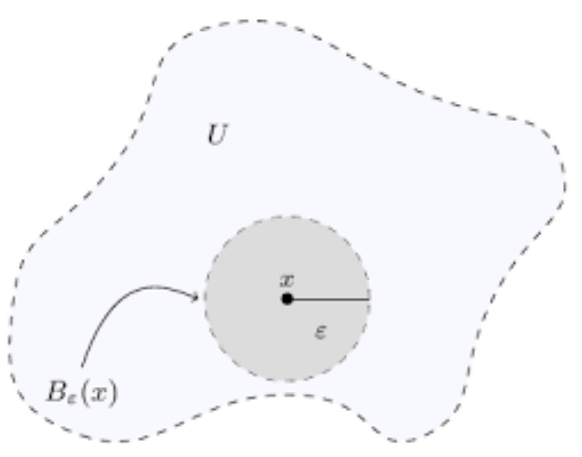
\includegraphics[width=8cm]{images/open_set.png}
    \caption{Open set}
\end{figure}
%\part{Calculus (Single Variable)}

%applications of calculus involving parametric, polar and vector functions

\chapter{Limits}
\section{Precise Definition of a Limit}
The reader is assumed to know how a limit is defined intuitively. However, this definition is imprecise: phrases such as ``$x$ is close to $a$'' and ``$f(x)$ gets closer and closer to $L$'' are vague. In order to be able to prove limits conclusively, we must make the definition of a limit precise.

\begin{definition}
Let $f(x)$ be a function defined on an open interval around $x_0$. We say that the \vocab{limit} of $f(x)$ as $x$ approaches $x_0$ is $L$, that is $\displaystyle\lim_{x \to x_0}f(x)=L$, if for every $\epsilon>0$ there exists $\delta > 0$ such that $\forall x \in \RR$, 
\[ 0<\absolute{x-x_0}<\delta \implies \absolute{f(x)-L}<\epsilon \] 
\end{definition} 

Visualising this graphically, as $\epsilon$ becomes smaller and smaller, there always exists a $\delta$ that satisfies the property that for any $x$ in the open interval $(x_0-\delta,x_0+\delta)$, the value of $f(x)$ lies in the interval $(L-\epsilon, L+\epsilon)$.

\begin{figure}[H]
	\centering
	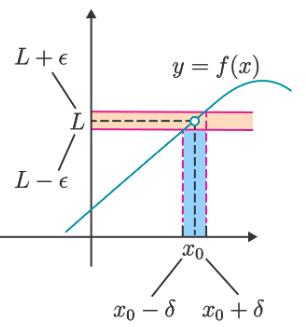
\includegraphics[width=0.3\linewidth]{images/Epsilon_delta_definition.png}
    \caption{Epsilon--delta definition}
\end{figure}

\begin{exercise}{}{} 
Prove that \[ \lim_{x\to3}2x+4=10. \]
\end{exercise}

Before the proof, we work backwards to find the value of $\delta$ in terms of $\epsilon$ and $x_0$, which we then declare in our proof.

$\forall \epsilon > 0$, $\exists \delta > 0$, $\forall x \in \RR$,
\[ |x-3| < \delta \implies |f(x)-10| < \epsilon \]
Let $\epsilon > 0$ be given.
\[ |f(x)-10| = |2x+4-10| = |2x-6| = 2|x-3| < \epsilon \]
Notice $|x-3| < \dfrac{\epsilon}{2}$. We can thus define $\delta \coloneqq \dfrac{\epsilon}{2}$. We now write our proof.

\begin{proof}
Let $\epsilon > 0$ be given. Choose $\delta = \dfrac{\epsilon}{2}$.

Then $\forall x \in \RR$, 
\begin{align*}
|x-3| &< \delta = \frac{\epsilon}{2} \\
2|x-3| &< \epsilon \\
|2x-6| &< \epsilon \\
|2x+4-10| &< \epsilon \\
|f(x)-10| &< \epsilon
\end{align*}
\end{proof}

\begin{exercise}{}{}
Use the formal definition of the limit to verify that 
\[ \lim_{x \to 3} \sqrt{2x+3} = 3. \]
\end{exercise}

We must prove that $\forall \epsilon > 0$, $\exists \delta > 0$ such that $\sqrt{2x+3} - 3 < \epsilon$ whenever $|x-3|<\delta$.
\begin{align*}
\sqrt{2x+3} - 3 &= \absolute{\frac{(2x+3)-3^2}{\sqrt{2x+3} + 3}} = \absolute{\frac{2x-6}{\sqrt{2x+3} + 3}} \\
&\le \absolute{\frac{2(x-3)}{3}} \\
&= \frac{2}{3} \absolute{x-3} < \frac{2}{3} \delta
\end{align*}
Hence, we can define 
\[ \epsilon \coloneqq \frac{2}{3} \delta \]
which we can use in our proof.

\begin{proposition}[Sum Law]
If $\lim_{x\to a}f(x)=L$ and $\lim_{x\to a}g(x)=M$ both exist, then
\[ \lim_{x\to a}[f(x)+g(x)]=L+M. \]
\end{proposition}

\begin{proof}
Let $\epsilon>0$ be given. We must find $\delta>0$ such that
\[ 0<|x-a|<\delta \implies |f(x)+g(x)-(L+M)|<\epsilon. \]
Using the Triangle Inequality we can write
\begin{align*}
\absolute{f(x)+g(x)-(L+M)}&=\absolute{\brac{f(x)-L}+\brac{g(x)-M}}\\
&\le|f(x)-L|+|g(x)-M|
\end{align*}
We make $\absolute{f(x)+g(x)-(L+M)}$ less than $\epsilon$ by making each of the terms $|f(x)-L|$ and $|g(x)-M|$ less than $\frac{\epsilon}{2}$.

Since $\frac{\epsilon}{2}>0$ and $\lim_{x\to a}f(x)=L$, there exists $\delta_1>0$ such that
\[ 0<|x-a|<\delta_1 \implies |f(x)-L|<\frac{\epsilon}{2}. \]
Similarly, since $\lim_{x\to a}g(x)=M$, there exists $\delta_2>0$ such that
\[ 0<|x-a|<\delta_2 \implies |g(x)-M|<\frac{\epsilon}{2}. \]
Let $\delta=\min\{\delta_1,\delta_2\}$, the smaller of the numbers $\delta_1$ and $\delta_2$. Notice that
\[ 0<|x-a|<\delta \implies 0<|x-a|<\delta_1 \text{ and } 0<|x-a|<\delta_2 \]
and so
\[ |f(x)-L|<\frac{\epsilon}{2} \text{ and } |g(x)-M|<\frac{\epsilon}{2}. \]
Therefore
\begin{align*}
\absolute{f(x)+g(x)-(L+M)}&\le|f(x)-L|+|g(x)-M|\\
&<\frac{\epsilon}{2}+\frac{\epsilon}{2}=\epsilon.
\end{align*}
To summarise,
\[ 0<|x-a|<\delta \implies \absolute{f(x)+g(x)-(L+M)}<\epsilon. \]
Thus by the definition of a limit,
\[ \lim_{x\to a}[f(x)+g(x)]=L+M. \]
\end{proof}
\pagebreak

\section{Limit Laws}
Let $f(x)$ and $g(x)$ be defined for all $x\neq a$ over some open interval containing $a$. Assume that $L$ and $M$ are real numbers such that $\lim_{x\to a}f(x)=L$ and $\lim_{x\to a}g(x)=M$, $c$ is a constant. Then each of the following statements holds.

\begin{itemize}
\item \textbf{Sum law}: The limit of a sum is the sum of the limits.
\[ \lim_{x\to a}(f(x)+g(x)) = \lim_{x\to a}f(x) + \lim_{x\to a}g(x) = L+M \]

\item \textbf{Difference law}: The limit of a difference is the difference of the limits.
\[ \lim_{x\to a}(f(x)-g(x)) = \lim_{x\to a}f(x) - \lim_{x\to a}g(x) = L-M \]

\item \textbf{Constant multiple law}: The limit of a constant times a function is the constant times the limit of the function.
\[ \lim_{x\to a}cf(x) = c\lim_{x\to a}f(x) = cL \]

\item \textbf{Product law}: The limit of a product is the product of the limits.
\[ \lim_{x\to a}(f(x)\cdot g(x)) = \lim_{x\to a}f(x) \cdot \lim_{x\to a}g(x) = L\cdot M \]

\item \textbf{Quotient law}: The limit of a quotient is the quotient of the limits.
\[ \lim_{x\to a}\frac{f(x)}{g(x)} = \frac{\lim_{x\to a}f(x)}{\lim_{x\to a}g(x)} = \frac{L}{M} \]
for $M \neq 0$.

\item \textbf{Power law}
\[ \lim_{x\to a}(f(x))^n = (\lim_{x\to a}f(x))^n = L^n \]
for every positive integer $n$.

\item \textbf{Root law}
\[ \lim_{x\to a}\sqrt[n]{f(x)} = \sqrt[n]{\lim_{x\to a}f(x)} = \sqrt[n]{L} \]
for all $L$ if $n$ is odd, and for $L\ge 0$ if $n$ is even.
\end{itemize}
\pagebreak

\section{Evaluating Limits}
Indeterminate forms of a limit include:
\[ \frac{0}{0} \quad \frac{\infty}{\infty} \quad 0 \times \infty \quad \infty - \infty \quad 0^0 \quad 1^{\infty} \quad \infty^0 \]
As long as limits are in indeterminate forms, they can still be evaluated.

Methods:
\begin{itemize}
\item Direct substitution

If $f$ is a polynomial or a rational function and $a$ is in the domain of $f$, then
\[ \lim_{x\to a}f(x)=f(a) \]

\item Cancel common factors
\item Multiply by the conjugate of the numerator or denominator
\end{itemize}

\begin{exercise}{}{}
Evaluate the following limit:
\[ \lim_{x\to 0} x^2\sin\brac{\frac{1}{x}} \]
\end{exercise}

\begin{solution}
If we plot the graph of the function out, we see that we can try to find two functions to apply Squeeze Theorem.

Notice that \[ -1 \le \sin\brac{\frac{1}{x}} \le 1 \]
and hence
\[ -x^2 \le x^2\sin\brac{\frac{1}{x}} \le x^2 \]
thus $x^2$ and $-x^2$ are the two functions that ``sandwich'' the given function.

Since $\lim_{x\to 0}x^2=0$ and $\lim_{x\to 0}-x^2=0$, applying Squeeze Theorem gives us 
\[ \lim_{x\to 0} x^2\sin\brac{\frac{1}{x}} = 0 \]
\end{solution}

\begin{exercise}{}{}
Evaluate the following limit:
\[ \lim_{x\to 3}\frac{-4x}{x-3} \]
\end{exercise}

\begin{solution}
Approaching from the left side,
\[ \lim_{x\to 3^-}\frac{-4x}{x-3} = +\infty \]
Approaching from the right side,
\[ \lim_{x\to 3^+}\frac{-4x}{x-3} = -\infty \]
Since $\lim_{x\to 3^-}\dfrac{-4x}{x-3} \neq \lim_{x\to 3^+}\dfrac{-4x}{x-3}$, the limit does not exist.
\end{solution}

\begin{theorem}
If $f(x) \le g(x)$ when $x$ is near $a$ (except possibly at $a$) and the limits of $f$ and $g$ both exist as $x$ approaches $a$, then
\[ \lim_{x\to a}f(x) \le \lim_{x\to a}g(x). \]
\end{theorem}

\begin{theorem}[Squeeze theorem]
Suppose that $g(x) \ge f(x) \ge h(x)$ for all $x$ in some open interval containing $c$ except possibly at $c$ itself. If $\lim_{x\to c} g(x) = L = \lim_{x\to c} h(x)$, then $\lim_{x\to c} f(x) = L$.
\end{theorem}

\begin{proof}
This can be proven using the epsilon--delta definition of limits.

Let $\epsilon > 0$ be given. We are done if we find a $\delta > 0$ such that $|f(x)-L| < \epsilon$ whenever $0 < |x-c| < \delta$.

Since $\lim_{x\to c} g(x) = L$, by definition of limits, there exists some $\delta_1 > 0$ such that for all $0 < |x-c| < \delta_1$, $|g(x)-L| < \epsilon$.
Thus, 
\[ -\epsilon < g(x)-L < \epsilon \quad \text{for all } 0 < |x-c| < \delta_1 \]
so
\begin{equation*}\tag{1}
L-\epsilon < g(x) < L + \epsilon \quad \text{for all } 0 < |x-c| < \delta_1
\end{equation*}
Similarly, since $\lim_{x\to c} h(x) = L$, by definition of limits, there exists some $\delta_2 > 0$ such that
\begin{equation*}\tag{2}
L-\epsilon < h(x) < L + \epsilon \quad \text{for all } 0 < |x-c| < \delta_2
\end{equation*}
Additionally, since $g(x) \le f(x) \le h(x)$ for all $x$ in some open interval containing $c$, there exists some $\delta_3 > 0$ such that for 
\begin{equation*}\tag{3}
g(x) \le f(x) \le h(x) \quad \text{for all } 0 < |x-c| < \delta_3
\end{equation*}
Now, we choose $\delta = \min(\delta_1, \delta_2, \delta_3)$. Then by (1), (3), and (2), we have 
\[ L-\epsilon < g(x) \le f(x) \le h(x) < L + \epsilon \quad \text{for all } 0 < |x-c| < \delta. \]
Therefore, $-\epsilon < f(x)-L < \epsilon$ for all $0 < |x-c| < \delta$, so
\[ |f(x)-L| < \epsilon \quad \text{for all } 0 < |x-c| < \delta. \]
Hence, by definition of limits, $\lim_{x\to c} f(x) = L$.
\end{proof}

\begin{theorem}[L'H\^{o}pital's Rule]
Let $f(x)$ and $g(x)$ be differentiable on an interval $I$ containing $c$, and that $g^\prime(c)\neq0$ on $I$ for $x \neq c$. Suppose that $\lim_{x\to c}\frac{f(x)}{g(x)}$ is in an indeterminate form. 

Then as long as the limits exist, we have 
\[ \lim_{x\to c}\frac{f(x)}{g(x)} = \lim_{x\to c}\frac{f^\prime(x)}{g^\prime(x)}. \]
\end{theorem}

\begin{proof}

\end{proof}

\begin{exercise}{}{}
Let $f$ be a differentiable function on $(0,\infty)$ and suppose that $\lim_{x\to\infty}\brac{f(x)+f^\prime(x)}=L$.

By considering $f(x)=\dfrac{e^xf(x)}{e^x}$, show that $\lim_{x\to\infty}f(x)=L$ and $\lim_{x\to\infty}f^\prime(x)=0$.
\end{exercise}

\begin{solution}
We may apply L'H\^{o}pital's Rule as we encounter $\dfrac{\infty}{\infty}$ in $\displaystyle\lim_{x\to\infty}\frac{e^xf(x)}{e^x}$.

\[ \lim_{x\to\infty}f(x)=\lim_{x\to\infty}\frac{e^xf(x)}{e^x}=\lim_{x\to\infty}\frac{\brac{e^xf(x)}^\prime}{\brac{e^x}^\prime}=\lim_{x\to\infty}\frac{e^xf(x)+e^xf^\prime(x)}{e^x}=L \]

Hence $\lim_{x\to\infty}f(x)=L$ and $\lim_{x\to\infty}f^\prime(x)=0$.
\end{solution}
\pagebreak

% uniqueness of the limit


\section{Important Limits}
\begin{equation}
\lim_{x \to 0} \frac{\sin x}{x} = 1
\end{equation}
\begin{proof}
This can be proven using the squeeze theorem, which will be discussed later.
\end{proof}

\begin{equation}
\lim_{x \to 0} \frac{1-\cos x}{x} = 0
\end{equation}
\begin{proof}
This can be proven using the squeeze theorem, which will be discussed later.
\end{proof}

\begin{equation}
\lim_{x\to 0} \frac{\arcsin x}{x} = 1
\end{equation}

\begin{equation}
\lim_{x\to \pm\infty} \brac{1+\frac{1}{x}}^x=e
\end{equation}
\pagebreak

\section{Continuity}
\begin{definition}
A function $f(x)$ is \vocab{continuous} at $x=a$ if 
\[ \lim_{x\to a} f(x)=f(a). \]
A function is said to be continuous on the interval $[a,b]$ if it is continuous at each point in the interval.
\end{definition}

Note that this definition is also implicitly assuming that both $f(a)$ and $\lim_{x\to a}f(x)$ exist. If either of these do not exist the function will not be continuous at $x=a$.

This definition can be turned around into the following fact.
\begin{corollary}
If $f(x)$ is continuous at $x=a$ then
\[ \lim_{x \to a} f(x) = f(a) \quad \lim_{x \to a^-} f(x) = f(a) \quad \lim_{x \to a^+} f(x) = f(a) \]
\end{corollary}

A nice consequence of continuity is the following fact.
\begin{corollary}
If $f(x)$ is continuous at $x=b$ and $\lim_{x\to a}g(x)=b$ then
\[ \lim_{x \to a} f(g(x)) = f\brac{\lim_{x \to a} g(x)} \]
\end{corollary}

\begin{exercise}{}{}
Evaluate the following limit:
\[ \lim_{x \to 0} e^{\sin x} \]
\end{exercise}

\begin{solution}
Since we know that exponentials are continuous everywhere we can use the fact above.
\[ \lim_{x \to 0} e^{\sin x} = e^{\lim_{x \to 0} \sin x} = e^0 = \boxed{1} \]
\end{solution}

Another very nice consequence of continuity is the Intermediate Value Theorem.
\begin{theorem}[Intermediate Value Theorem]
Suppose that $f(x)$ is continuous on $[a,b]$ and let $M$ be any number between $f(a)$ and $f(b)$. Then there exists $c \in (a,b)$ such that $f(c)=M$.
\end{theorem}
All the Intermediate Value Theorem is really saying is that a continuous function will take on all values between $f(a)$ and $f(b)$.
\pagebreak

\chapter{Derivative}
\section{Definitions}
\begin{definition}
The \vocab{derivative} of $f(x)$ with respect to $x$, denoted by $f^\prime(x)$, is defined as 
\begin{equation} f^\prime (x) = \lim_{h \to 0} \frac{f(x+h)-f(x)}{h}.
\end{equation}
\end{definition}

The right-hand derivative of $f(x)$ at $x=x_0$ is defined as
\[ f_+^\prime(x_0)=\lim_{h\to0^+}\frac{f(x_0+h)-f(x_0)}{h}. \]
Similarly, the left-hand derivative of $f(x)$ at $x=x_0$ is defined as
\[ f_-^\prime(x_0)=\lim_{h\to0^-}\frac{f(x_0+h)-f(x_0)}{h}. \]
A function $f$ has a derivative at $x=x_0$ if and only if $f_+^\prime(x_0)=f_-^\prime(x_0)$.

\begin{definition} 
$f(x)$ is \vocab{differentiable} at $x_0$ if $f^\prime(x_0)$ exists; $f(x)$ is differentiable on an interval $I$ if the derivative exists for every $x\in I$.
\end{definition}

\begin{theorem}
$f(x)$ is continuous at $x_0$ if $f(x)$ is differentiable at $x=x_0$.
\end{theorem}

\begin{proof}
To prove that $f$ is continuous at $x_0$, we have to show that $\lim_{x\to x_0}f(x)=f(x_0)$. We will do this by showing that the difference $f(x)-f(x_0)$ approaches $0$.

Given that $f$ is differentiable at $x_0$,
\[ f^\prime(x_0)=\lim_{x\to x_0}\frac{f(x)-f(x_0)}{x-x_0} \]
exists. We can rewrite
\[ f(x)-f(x_0)=\frac{f(x)-f(x_0)}{x-x_0}(x-x_0). \]
Then
\begin{align*}
\lim_{x\to x_0}[f(x)-f(x_0)]
&=\lim_{x\to x_0}\frac{f(x)-f(x_0)}{x-x_0}(x-x_0)\\
&=\lim_{x\to x_0}\frac{f(x)-f(x_0)}{x-x_0}\cdot\lim_{x\to x_0}(x-x_0)\\
&=f^\prime(x_0)\cdot0=0
\end{align*}
To use what we have just proved, 
\begin{align*}
\lim_{x\to x_0}f(x)
&=\lim_{x\to x_0}[f(x_0)+\brac{f(x)-f(x_0)}]\\
&=\lim_{x\to x_0}f(x_0)+\lim_{x\to x_0}[f(x)-f(x_0)]\\
&=f(x_0)+0=f(x_0)
\end{align*}
Therefore $f$ is continuous at $x_0$.
\end{proof}

\begin{remark}
This means differentiability implies continuity. However the converse is not necessarily true, one notable example being the Weierstrass function.
\end{remark}
\pagebreak

\section{Theorems}
\begin{definition}
Let $c$ be a number in the domain $D_f$ of a function $f$. Then $f(c)$ is the
\begin{itemize}
\item \vocab{absolute maximum} value of $f$ on $D_f$ if $f(c)\ge f(x)$ for all $x\in D_f$.
\item \vocab{absolute minimum} value of $f$ on $D_f$ if $f(c)\le f(x)$ for all $x\in D_f$.
\end{itemize}
\end{definition}

An absolute maximum or minimum is sometimes called a \emph{global} maximum or minimum. The maximum and minimum values of $f$ are called \vocab{extreme values} of $f$.

\begin{definition}
$f(c)$ is a
\begin{itemize}
\item \vocab{local maximum} value of $f$ if $f(c)\ge f(x)$ when $x$ is near $c$.
\item \vocab{local minimum} value of $f$ if $f(c)\le f(x)$ when $x$ is near $c$.
\end{itemize}
\end{definition}

We have seen that some functions have extreme values, whereas others do not. The following theorem gives conditions under which a function is guaranteed to possess extreme values.

\begin{theorem}[Extreme Value Theorem]
For a function $f$ continuous on $[a,b]$, it attains its maximum and minimum values on $[a,b]$.
\end{theorem}

\begin{proof}
We prove the case that $f$ attains its maximum value on $[a,b]$.

Since $f$ is continuous on $[a,b]$, we know it must be bounded on $[a,b]$ by the Boundedness Theorem. Let $M = \sup f$.

If there is some $c \in [a,b]$ where $f(c)=M$ there is nothing more to show -- $f$ attains its maximum on $[a,b]$.

Suppose otherwise, that there is no such $c$. Then $f(x)<M$ for all $x \in [a,b]$.

We define a new function $g$ by 
\[ g(x) = \frac{1}{M-f(x)}. \]

Note that $g(x)>0$ for every $x \in [a,b]$ and $g$ is continuous on $[a,b]$, and thus also bounded on this interval, again by the Boundedness theorem.

Given that $g$ is bounded on $[a,b]$, there must exist some $K>0$ such that $g(x) \le K$ for every $x \in [a,b]$.

Consequently,
\[ \frac{1}{M-f(x)} \le K \implies f(x) \le M - \frac{1}{K} \]
for every $x \in [a,b]$. This contradicts the assumption that $M$ is the least upper bound.

That leaves as the only possibility that there is some $c$ in $[a,b]$ where $f(c)=M$. That is to say, $f$ attains its maximum on $[a,b]$.

The proof that $f$ attains its minimum on the same interval is argued similarly and is left as an exercise for the reader.
\end{proof}

\begin{theorem}[Fermat's Theorem]
If $f$ has a local maximum or minimum at $c$, and if $f^\prime(c)$ exists, then $f^\prime(c)=0$.
\end{theorem}

\begin{proof}
Suppose, for the sake of definiteness, that $f$ has a local maximum at $c$. Then $f(c)\ge f(x)$ if $x$ is sufficiently close to $c$. This implies that if $h$ is sufficiently close to $0$, with $h$ being positive or negative, then
\[ f(c)\ge f(c+h) \]
and thus
\[ f(c+h)-f(c)\le0. \]
We can divide both sides of an inequality by a positive number. Thus, if $h>0$ and $h$ is sufficiently small, we have
\[ \frac{f(c+h)-f(c)}{h}\le0. \]
Taking the right-hand limit of both sides of the inequality,
\[ \lim_{h\to0^+}\frac{f(c+h)-f(c)}{h}\le\lim_{h\to0^+}0=0 \]
but since $f^\prime(c)$ exists, we have
\[ f^\prime(c)=\lim_{h\to0}\frac{f(c+h)-f(c)}{h}=\lim_{h\to0^+}\frac{f(c+h)-f(c)}{h} \]
and so we have show that $f^\prime(c)\le0$.

On the other hand, if $h<0$, then the direction of the inequality is reversed when we divide by $h$:
\[ \frac{f(c+h)-f(c)}{h}\ge0 \]
so taking the left-hand limit, we have
\[ f^\prime(c)=\lim_{h\to0}\frac{f(c+h)-f(c)}{h}=\lim_{h\to0-}\frac{f(c+h)-f(c)}{h}\ge0 \]
thus $f^\prime(c)\ge0$.

Since $f^\prime(c)\ge0$ and $f^\prime(c)\le0$, we have $f^\prime(c)=0$.

We have proved Fermat's Theorem for the case of a local maximum. The case of a local minimum can be proved in a similar manner.
\end{proof}

\begin{theorem}[Rolle's Theorem]
Let $f:[a,b]\to\RR$ be continuous on $[a,b]$ and differentiable on $(a,b)$, and $f(a)=f(b)$. Then there exists $c \in (a,b)$ such that 
\[ f^\prime(c)=0. \]
\end{theorem}
\begin{remark}
Rolle's Theorem is simply a special case of the Mean Value Theorem, where $f(a)=f(b)$.
\end{remark}

\begin{proof}
\textbf{Case 1:} $f(x)=k$ where $k$ is a constant

Then $f^\prime(x)=0$, so the number $c$ can be taken to be any number in $(a,b)$.

\textbf{Case 2:} $f(x)>f(a)$ for some $x\in(a,b)$

By the Extreme Value Theorem, $f$ has a maximum value somewhere in $[a,b]$. Since $f(a)=f(b)$, it must attain this maximum value at a number $c$ in the open interval $(a,b)$. Then $f$ has a local maximum at $c$, thus $f$ is differentiable at $c$. Therefore $f^\prime(c)=0$ by Fermat's Theorem.

\textbf{Case 3:} $f(x)<f(a)$ for some $x\in(a,b)$

By the Extreme Value Theorem, $f$ has a minimum value in $[a,b]$ and, since $f(a)=f(b)$, it attains this minimum value at a number $c\in(a,b)$. Again $f^\prime(c)=0$ by Fermat's Theorem.
\end{proof}

\begin{theorem}[Mean Value Theorem]
Let $f:[a,b]\to\RR$ be continuous on $[a,b]$ and differentiable on $(a,b)$. Then there exists $c\in(a,b)$ such that 
\[ f^\prime(c)=\frac{f(b)-f(a)}{b-a}. \]
\end{theorem}

\begin{figure}[H]
    \centering
    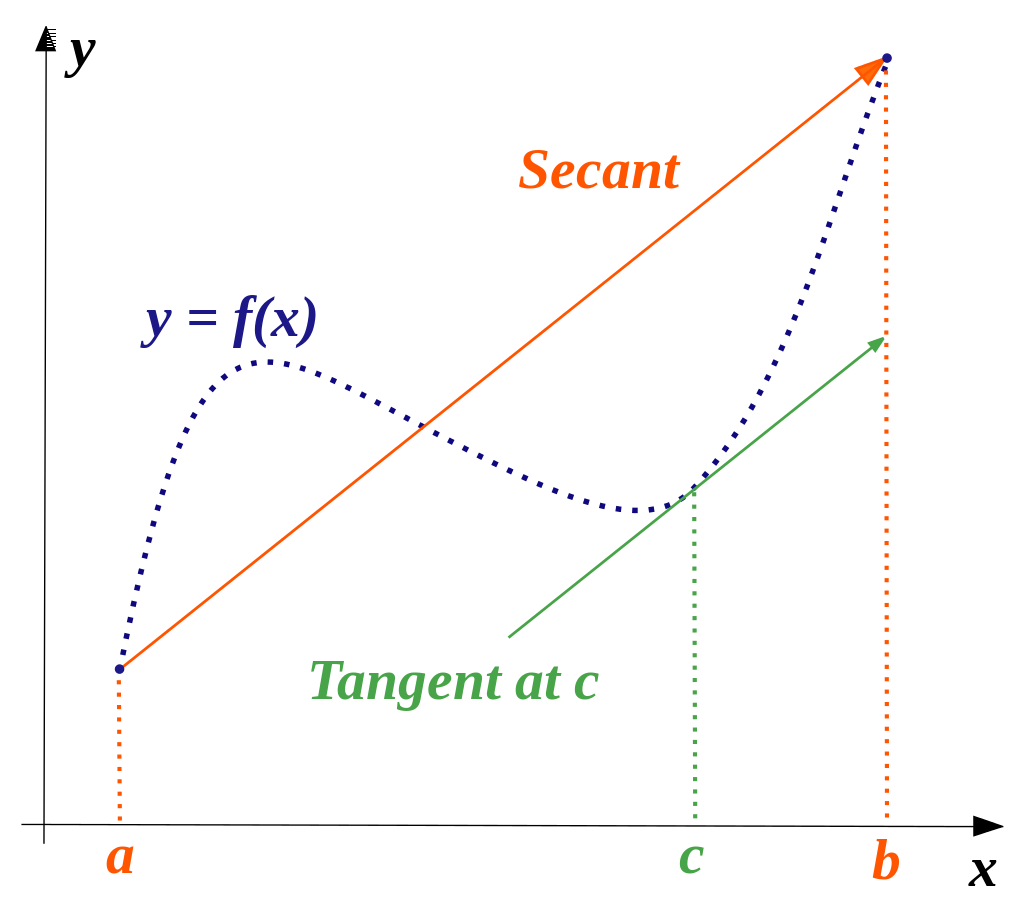
\includegraphics[width=8cm]{images/mean_value_thrm.png}
    \caption{Mean value theorem}
\end{figure}

\begin{theorem}[Cauchy's Generalised Theorem of the Mean]
Let $f$ and $g$ be continuous on $[a,b]$ and differentiable on $(a,b)$, and where $g(x)\neq0$ in $(a,b)$. Then there exists $c\in(a,b)$ such that
\[ \frac{f^\prime(c)}{g^\prime(c)}=\frac{f(b)-f(a)}{g(b)-g(a)}. \]
\end{theorem}

In layman's term, the theorem states that given two differentiable functions, there is some point $c$ where the ratio of their average rates of change agrees with the ratio of their instantaneous rates of change.

\begin{remark}
When $g(x)=x$, it reduces to the Mean Value Theorem.
\end{remark}

\begin{exercise}{}{}
Let $f(x)=\dfrac{x^e}{e^x}$, where $x>0$. Find the maximum value of $f(x)$ and hence prove that $e^\pi>\pi^e$.
\end{exercise}

\begin{proof}
\[ f^\prime(x)=x^{e-1}e^{-x}(e-x) \]
Since $x^{e-1}e^{-x}>0$ for all $x>0$, we have
\[ f^\prime(x)=\begin{cases}
>0 & x<e\\
0 & x=e\\
<0 & x>e
\end{cases}. \]
Hence the maximum value of $f$ occurs at $x=e$ since $f$ is a continuous function, with maximum value $f(e)=\dfrac{e^e}{e^e}=1$.

Therefore $\dfrac{x^e}{e^x}<1$ for all $x\in\RR^+\setminus\{e\}$, i.e. $\dfrac{\pi^e}{e^\pi}<1$ and thus $e^\pi>\pi^e$.
\end{proof}

\begin{exercise}{}{}
By applying Rolle's Theorem on the function $f(x)=e^{-x}-\sin x$, show that there is at least one real root of $e^x\cos x=-1$ between any two real roots of $e^x\sin x=1$.
\end{exercise}

\begin{proof}
Let the two real roots involved of $e^x\sin x=1$ be $a$ and $b$ with $a<b$.

Then $f(a)=f(b)=0$. By Rolle's Theorem, there exist a value $c$ with $a<c<b$ such that $f^\prime(c)=0$, i.e. $-e^{-c}-\cos c=0$ which reduces to $e^c\cos c=-1$.
\end{proof}

\begin{exercise}{}{}
By using the Theorem of the Mean, show that
\[ \frac{\pi}{6}+\frac{\sqrt{3}}{15}<\sin^{-1}0.6<\frac{\pi}{6}+\frac{1}{8}. \]
\end{exercise}

\begin{proof}
Let $f(x)=\sin^{-1}x$, we have $f^\prime(x)=\dfrac{1}{\sqrt{1-x^2}}$.

By the Theorem of the Mean, we have, for $a<c<b$,
\[ \frac{1}{\sqrt{1-a^2}}<\frac{1}{\sqrt{1-c^2}}=\frac{\sin^{-1}(b)-\sin^{-1}(a)}{b-a}<\frac{1}{\sqrt{1-b^2}}. \]
i.e. Interval min grad / Interval average grad/ Interval max grad

Using $a=0.5$ and $b=0.6$,
\begin{align*}
&\frac{1}{\sqrt{1-0.5^2}}<\frac{\sin^{-1}0.6-\sin^{-1}0.5}{0.6-0.5}<\frac{1}{\sqrt{1-0.6^2}} \\
&\frac{2}{\sqrt{3}}<\frac{\sin^{-1}0.6-\frac{\pi}{6}}{0.1}<\frac{1}{0.8} \\
&\frac{\sqrt{3}}{15}<\sin^{-1}0.6-\frac{\pi}{6}<\frac{1}{8} \\
&\frac{\pi}{6}+\frac{\sqrt{3}}{15}<\sin^{-1}0.6<\frac{\pi}{6}+\frac{1}{8}
\end{align*}
\end{proof}
\pagebreak

\section{Differentiation Rules}
For a constant $c\in\RR$ and functions $f$ and $g$ of $x$, the following rules hold.

\begin{itemize}
\item \textbf{Scalar multiplication}
\[ (cf)^\prime = cf^\prime \]

\item \textbf{Addition rule}
\[ (f+g)^\prime = f^\prime + g^\prime \]

\begin{proof}
\begin{align*}
(f + g)^\prime (x) &= \lim_{h \to 0} \frac{(f+g)(x+h) - (f+g)(x)}{h}\\
&= \lim_{h \to 0} \frac{f(x+h) + g(x+h) - f(x) - g(x)}{h}\\
&= \lim_{h \to 0} \left[ \frac{f(x+h) - f(x)}{h} + \frac{g(x+h) - g(x)}{h} \right] \\
&= \lim_{h \to 0} \frac{f(x+h) - f(x)}{h} + \lim_{h \to 0} \frac{g(x+h) - g(x)}{h}\\
&= f^\prime (x) + g^\prime (x)
\end{align*}
\end{proof}

\item \textbf{Power rule}
\[ \dv{x} x^n = n x^{n-1} \]

\begin{proof}
Using implicit differentiation,
\begin{align*}
y &= x^n \\
\ln y &= \ln x^n \\
\ln y &= n \ln x \\
\frac{y^\prime}{y} &= n \frac{1}{x}
\end{align*}
\[ y^\prime = y \frac{n}{x} = x^n \brac{\frac{n}{x}} = n x^{n-1} \]
\end{proof}

\item \textbf{Product rule}
\[ (fg)^\prime = f^\prime g + f g^\prime \]

\begin{proof}
\begin{align*}
(fg)^\prime (x) &= \lim_{h \to 0} \frac{(fg)(x+h) - (fg)(x)}{h}\\
&= \lim_{h \to 0} \frac{f(x+h) g(x+h) - f(x) g(x)}{h}\\
&= \lim_{h \to 0} \frac{f(x+h) g(x) - f(x) g(x) + f(x+h) g(x+h) - f(x+h) g(x)}{h}\\
&= \lim_{h \to 0} \frac{f(x+h) g(x) - f(x) g(x)}{h} + \lim_{h \to 0} \frac{f(x+h) g(x+h) - f(x+h) g(x)}{h}\\
&= \lim_{h \to 0} \frac{f(x+h) - f(x)}{h}g(x) + \lim_{h \to 0} \frac{g(x+h) - g(x)}{h}f(x+h)\\
&= \left[\lim_{h \to 0} \frac{f(x+h) - f(x)}{h}\right] g(x) + \left[\lim_{h \to 0} \frac{g(x+h) - g(x)}{h}\right] f(x)\\
&= f^\prime (x) g(x) + f(x) g^\prime (x)
\end{align*}
\end{proof}

\item \textbf{Quotient rule}
\[ \brac{\frac{f}{g}}^\prime = \frac{f^\prime g - fg^\prime}{g^2} \] 

\begin{proof}
\begin{align*}
\left[\frac{f(x)}{g(x)}\right]^\prime &= \lim_{h \to 0} \frac{\frac{f(x+h)}{g(x+h)} - \frac{f(x)}{g(x)}}{h}\\
&= \lim_{h \to 0} \frac{1}{h} \frac{f(x+h) g(x) - f(x) g(x+h)}{g(x+h) g(x)}\\
&= \lim_{h \to 0} \frac{1}{h} \frac{f(x+h) g(x) - f(x) g(x) + f(x) g(x) - f(x) g(x+h)}{g(x+h) g(x)}\\
&= \lim_{h \to 0} \frac{1}{g(x+h) g(x)} \left[ \frac{f(x+h)g(x) - f(x)g(x)}{h} + \frac{f(x)g(x) - f(x)g(x+h)}{h} \right] \\
&= \lim_{h \to 0} \frac{1}{g(x+h) g(x)} \left[ g(x)\frac{f(x+h) - f(x)}{h} - f(x)\frac{g(x) + g(x+h)}{h} \right] \\
&= \frac{1}{g^2(x)} [g(x) f^\prime(x) - f(x) g^\prime(x)] \\
&= \frac{f^\prime(x) g(x) - f(x) g^\prime(x)}{g^2(x)}
\end{align*}
\end{proof}

\item \textbf{Chain rule}
\begin{theorem}[Chain rule] 
If $f$ and $g$ are both differentiable functions and we define $F(x)=(f\circ g)(x)$, then the derivative of $F(x)$ is
\begin{equation}
F^\prime (x) = f^\prime(g(x)) g^\prime(x) 
\end{equation}
\end{theorem}
\end{itemize}

\section{Applications of Differentiation}
\subsection{Implicit differentiation}
\textbf{Implicit differentiation} simply means differentiating both sides of the equation with respect to a variable.

\subsection{Newton's Method}
In this section we are going to look at a method for approximating solutions to equations.

\begin{figure}[H]
    \centering
    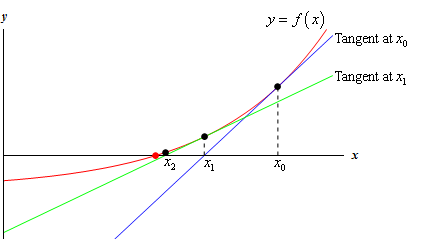
\includegraphics[width=10cm]{images/newton_method.png}
\end{figure}

Suppose that we want to approximate the solution to $f(x)=0$. Suppose that we have somehow found an initial rough approximation to the solution: $x=x_0$. The tangent line to $f(x)$ at $x=x_0$ is
\[ y = f(x_0) + f^\prime(x_0)(x-x_0) \]

This tangent line crosses the $x$-axis much closer to the actual solution to the equation than $x_0$ does. Let the tangent at $x_0$ intersect $x$-axis at $x_1$. We use this point as our new approximation to the solution. $x_1$ is given by:
\[ x_1 = x_0 - \frac{f(x_0)}{f^\prime(x_0)} \]

Repeat the process; form up the tangent line at $x_1$ and use its root $x_2$ as a new approximation:
\[ x_2 = x_1 - \frac{f(x_1)}{f^\prime(x_1)} \]

Here is the general Newton's Method:
\begin{thrm}{Newton's Method}{}
If $x_n$ is an approximation of a solution of $f(x)=0$ and if $f^\prime(x_n) \neq 0$, then the next approximation is given by
\[ x_{n+1} = x_n - \frac{f(x_n)}{f^\prime(x_n)} \]
\end{thrm}
\pagebreak

\chapter{Integral}
\section{Definition}
We use the \textbf{Riemann} definition of an integral:
\begin{definition}
An \vocab{integral} is defined as an infinite sum over an interval.
\begin{equation}
\int_a^b f(x) \dd{x} = \lim_{n \to \infty} \sum_{i=1}^n f(x_i) \Delta x
\end{equation}
\end{definition}

A Riemann sum is an approximation of an integral by a finite sum.

Let $f$ be defined on the closed interval $[a,b]$ and let $\Delta x$ be a partition of $[a,b]$, with
\[ a=x_1 < x_2 < \cdots < x_n < x_{n+1}=b.\]

Let $\Delta x_i$ denote the length of the $i$th subinterval $[x_i,x_{i+1}]$ and let $c_i$ denote any value in the $i$th subinterval.

The sum
\[ \sum_{i=1}^n f(c_i)\Delta x_i\]
is a Riemann sum of $f$ on $[a,b]$.

As the subinterval becomes infinitesimally small, 
\[ \int _{a}^{b}f(x) \dd{x} = \lim _{\Delta x \to 0} \sum _{i=1}^{n} f(x_{i}) \Delta x_{i} \]

\begin{figure}[H]
	\centering
	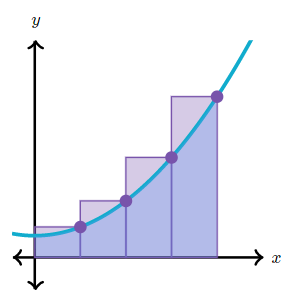
\includegraphics[width=8cm]{Riemanns_sums}
\end{figure}

\begin{thrm}{Fundamental Theorem of Calculus}{}
The fundamental theorem of (single variable) calculus states that if $f^\prime$ is continuous on $[a,b]$, then the integral of the derivative across the bounds is equal to the original function at the bounds:
\begin{equation}
\int_a^b f^\prime(x) \dd{x} = f(b)-f(a)
\end{equation}
or equivalently,
\begin{equation}
\dv{x} \int_{a}^{x} f(s) \dd{s} = f(x)
\end{equation}
\end{thrm}

% https://www2.clarku.edu/faculty/djoyce/ma121/FTCproof.pdf

Using the definition of the derivative, we differentiate the following integral:
\begin{align*}
\dv{x} \int_{a}^{x} f(s) \dd{s} &= \lim_{h \to 0} \frac{\int_{a}^{x+h} f(s) \dd{s} - \int_{a}^{x} f(s) \dd{s}}{h}\\
&= \lim_{h \to 0} \frac{\int_{x}^{x+h} f(s) \dd{s}}{h}\\
&= \lim_{h \to 0} \frac{h f(x)}{h}\\
&= f(x)
\end{align*}
% https://math.libretexts.org/Bookshelves/Calculus/Calculus_3e_(Apex)/05%3A_Integration/5.04%3A_The_Fundamental_Theorem_of_Calculus

\section{Integration Rules}
For constant $k\in\RR$ and functions $f(x)$ and $g(x)$, the following rules hold.
\begin{itemize}
\item \textbf{Sum and difference rule}
\[ \int f(x)\pm g(x) \dd{x} = \int f(x) \dd{x} \pm \int g(x) \dd{x} \]

\item \textbf{Scalar multiplication}
\[ \int kf(x) \dd{x} = k\int f(x) \dd{x} \]

\item \textbf{Power rule}
\[ \int x^n \dd{x} = \frac{x^{n+1}}{n+1} + C \]

\item \textbf{Constant rule}
\[ \int a\dd{x} = ax + C \]
\end{itemize}

\section{Integration Techniques}
\subsubsection{Integrals of powers and of trigonometric functions}
Reciprocal rules:
\[ \int \frac{1}{x} \dd{x} = \ln|x| + C \]
\[ \int \frac{1}{ax+b} \dd{x} = \frac{1}{a} \ln(ax+b) + C \]

Exponential functions:
\[ \int e^x \dd{x} = e^x + C \]
\[ \int a^{x} \dd{x} = \frac{a^x}{\ln a} + C \]

Natural log rule:
\[ \int \ln x \dd{x} = x\ln x - x + C \]

Trigonometric functions:
\[ \int \sin x \dd{x} = -\cos x + C \]

\[ \int \cos x \dd{x} = \sin x + C \]

\[ \int \tan x \dd{x} = \ln|\sec x| + C \]

\[ \int \cosec x \dd{x} = \ln|\cosec x - \cot x| + C \]

\[ \int \cosec^2x \dd{x} = -\cot x + C \]

\[ \cosec x \cot x \dd{x} = -\cosec x + C \]

\[ \sec x \dd{x} = \ln|\sec x + \tan x| + C \]

\[ \int \sec^2 x \dd{x} = \tan x + C \]

\[ \int \sec x \tan x \dd{x} = \sec x + C \]

\[ \int \cot x \dd{x} = \ln|\sin x| + C \]

Inverse trigonometric functions:
\[ \int\frac{1}{\sqrt{1-x^2}}\dd{x} = \sin^{-1}x + C \]
\[ \int-\frac{1}{\sqrt{1-x^2}}\dd{x} = \cos^{-1}x + C \]
\[ \int\frac{x}{1+x^2}\dd{x} = \tan^{-1}x + C \]

\subsubsection{Splitting the Numerator}
\begin{exercise}{}{}
Evaluate exactly
\[ \int_0^1\frac{x+2}{\sqrt{x+1}}\dd{x}. \]
\end{exercise}
\begin{solution}
\begin{align*}
\int_0^1\frac{x+2}{\sqrt{x+1}}\dd{x}
&= \int_0^1\brac{\sqrt{x+1}+\frac{1}{\sqrt{x+1}}}\dd{x} \\
&= \sqbrac{\frac{2}{3}(x+1)^\frac{3}{2}+2(x+1)^\frac{1}{2}}_0^1 \\
&= \boxed{\frac{2}{3}\brac{5\sqrt{3}-4}}
\end{align*}
\end{solution}

\subsubsection{Substitution}
\begin{equation}
\int f(g(x)) g^\prime (x)\dd{x} = \int f(u) \dd{u}
\end{equation}
where $u=g(x)$.

The most common way of doing a integral by substitution, and the only way for indefinite integrals, is as follows:
\begin{enumerate}
\item Change variables from $x$ to $u$ (hence the common name ``$u$-substitution'')
\item Keep track of the relation between $\dd{x}$ and $\dd{u}$
\item If you chose correctly you can now do the $u$-integral
\item When you are done, substitute back for $x$
\end{enumerate}

\begin{exercise}{}{}
Compute $\int\sin^nx\cos x\dd{x}$.
\end{exercise}
\begin{solution}
Substitute $u = \sin x$ and $\dd{u} = \cos x\dd{x}$. This turns the integral into $\int u^n\dd{u}$ which is easily valuated as $u^{n+1}/(n+1)$. Now plug back in $u = \sin x$ and you get the answer
\[ \frac{\sin^{n+1}x}{n+1}. \]
\end{solution}

\begin{exercise}{}{}
Compute $\displaystyle\int_1^2\frac{x}{x^2+1}\dd{x}$.
\end{exercise}
\begin{solution}
Let $u=x^2+1$ then $\dd{u} = 2x\dd{x}$, so the integrand becomes $(1/2)\dd{u}/u$. If $x$ goes
from 1 to 2 then $u$ goes from 2 to 5, thus the integral becomes
\[ \int_2^5\frac{1}{2}\frac{\dd{u}}{u} = \frac{1}{2}(\ln5-\ln2). \]
\end{solution}

\begin{exercise}{}{}
Compute $\int xe^{x^2}\dd{x}$.
\end{exercise}
\begin{solution}
To do this integral we'll use the following substitution.
\[ u=x^2 \implies \dd{u}=2x\dd{x} \implies x\dd{x}=\frac{1}{2}\dd{u} \]
\[ \int x e^{x^2}\dd{x} = \frac{1}{2}\int e^u \dd{u} = \frac{1}{2}e^u + c = \frac{1}{2}e^{x^2} + c \]
\end{solution}

\begin{exercise}{}{}
Prove the following result for $a>0$:
\begin{equation*}\tag{*}
\int_0^af(x)\dd{x}=\int_0^af(a-x)\dd{x}
\end{equation*}
Hence evaluate
\begin{enumerate}[label=(\alph*)]
\item $\displaystyle\int_0^\frac{\pi}{2}\frac{\cos^nx}{\sin^nx+\cos^nx}\dd{x}$, where $n$ is a real constant,
\item $\displaystyle\int_0^a\frac{x^4}{x^4+(x-a)^4}\dd{x}$, where $a$ is a positive real constant.
\end{enumerate}
\end{exercise}
\begin{solution}
Substitute $x=a-u\implies\dv{x}{u}=-1$.

For the lower and upper limits, $x=0\implies u=a$ and $x=a\implies u=0$ respectively.

Using the substitution, we have
\[ \int_0^af(x)\dd{x}=\int_a^0f(a-u)(-1)\dd{u}=\int_0^af(a-u)\dd{u}=\int_0^af(a-x)\dd{x}. \]

\begin{enumerate}[label=(\alph*)]
\item For $f(x)=\dfrac{\cos^nx}{\sin^nx+\cos^nx}$ with $a=\frac{\pi}{2}$,
\[ f\brac{\frac{\pi}{2}-x}=\frac{\cos^n\brac{\frac{\pi}{2}-x}}{\sin^n\brac{\frac{\pi}{2}-x}+\cos^n\brac{\frac{\pi}{2}-x}}=\frac{\sin^nx}{\cos^nx+\sin^nx}. \]
By (*), 
\[ \int_0^\frac{\pi}{2}f(x)\dd{x}=\int_0^\frac{\pi}{2}f\brac{\frac{\pi}{2}-x}\dd{x} \]
So we have
\[ \int_0^\frac{\pi}{2}\frac{\cos^nx}{\sin^nx+\cos^nx}\dd{x}=\int_0^\frac{\pi}{2}\frac{\sin^nx}{\sin^nx+\cos^nx}\dd{x} \]
Let $\displaystyle I=\int_0^\frac{\pi}{2}\frac{\cos^nx}{\sin^nx+\cos^nx}\dd{x}=\int_0^\frac{\pi}{2}\frac{\sin^nx}{\sin^nx+\cos^nx}\dd{x}$.

Then
\[ 2I=I+I=\int_0^\frac{\pi}{2}\frac{\sin^nx+\cos^nx}{\sin^nx+\cos^nx}\dd{x}=\int_0^\frac{\pi}{2}1\dd{x}=\frac{\pi}{2} \]
Hence $\displaystyle I=\int_0^\frac{\pi}{2}\frac{\cos^nx}{\sin^nx+\cos^nx}\dd{x}=\boxed{\frac{\pi}{4}}$

\item Let $f(x)=\dfrac{x^4}{x^4+(x-a)^4}$.

Then $f(a-x)=\frac{(a-x)^4}{(a-x)^4+(-x)^4}=\frac{(x-a)^4}{x^4+(x-a)^4}$.

By (*),
\[ I=\int_0^a\frac{x^4}{x^4+(x-a)^4}\dd{x}=\int_0^a\frac{(x-a)^4}{x^4+(x-a)^4}\dd{x} \]

Similarly, 
\[ 2I=\int_0^a\frac{x^4+(x-a)^4}{x^4+(x-a)^4}\dd{x}=\int_0^a1\dd{x}=a \]
Hence $I=\boxed{\frac{a}{2}}$
\end{enumerate}
\end{solution}

\subsubsection{Integration by parts}
Recall that the product rule for differentiation is given by
\[ (fg)^\prime=fg^\prime+f^\prime g. \]
Integrating both sides and rearranging gives us
\begin{equation}
\int f g^\prime\dd{x} = fg - \int f^\prime g\dd{x}
\end{equation}
Alternatively, we can rewrite this as 
\begin{equation}
\int u \dd{v} = uv - \int v \dd{u}
\end{equation}

DI method

Note that after applying integration by parts multiple times, we may obtain a multiple of the original integral. A simple rearrangement of the integral gives the required solution.

\begin{exercise}{}{}
Evaluate $\int e^x\cos x\dd{x}$.
\end{exercise}
\begin{solution}
Integrating by parts twice,
\begin{align*}
\int e^x\cos x\dd{x}
&= e^x\cos x-\int(e^x)(-\sin x)\dd{x}=e^x\cos x+\int e^x\sin x\dd{x} \\
&= e^x\cos x+\brac{e^x\sin x-\int e^x\cos x\dd{x}}
\end{align*}
Rearranging terms gives us
\[ 2\int e^x\cos x\dd{x}=e^x\cos x+e^x\sin x+c \]
Hence $\displaystyle\int e^x\cos x\dd{x}=\boxed{\frac{1}{2}\brac{e^x\cos x+e^x\sin x}+C}$
where $c$ and $C$ are arbitrary constants.
\end{solution}

Finally in this section we look at an example of a \textbf{reduction formula}.

\begin{exercise}{}{}
Consider $I_n=\int\cos^nx\dd{x}$ where $n$ is a non-negative integer. Find a reduction formula for $I_n$ and then use this formula to evaluate $\int\cos^7x\dd{x}$.
\end{exercise}
\begin{solution}
The aim here is to write $I_n$ in terms of other $I_k$ where $k<n$, so that eventually we are reduced to calculating $I_0$ or $I_1$, say, both of which are easily found. Using integration by parts we have:
\begin{align*}
I_n &= \int\cos^{n-1}x \times \cos x\dd{x} \\
&= \cos^{n-1}x\sin x-\int(n-1)\cos^{n-2}x(-\sin x)\sin x\dd{x} \\
&= \cos^{n-1}x\sin x+(n-1)\int\cos^{n-2}x(1-\cos^2x)\dd{x} \\
&= \cos^{n-1}x\sin x+(n-1)(I_{n-2}-I_n)
\end{align*}
Rearranging this to make $I_n$ the subject we obtain
\[ I_n=\frac{1}{n}\cos^{n-1}x\sin x+\frac{n-1}{n}I_{n-2}, \quad n\ge2. \]
With this reduction formula, $I_n$ can be rewritten in terms of simpler and simpler integrals until we are left only needing to calculate $I_0$ if $n$ is even, or $I_1$ if $n$ is odd.

Therefore, $I_7$ can be found as follows:
\begin{align*}
I_7 &= \frac{1}{7}\cos^6x\sin x+\frac{6}{7}I_5 \\
&= \frac{1}{7}\cos^6x\sin x+\frac{6}{7}\brac{\frac{1}{5}\cos^4x\sin x+\frac{4}{5}I_3} \\
&= \frac{1}{7}\cos^6x\sin x+\frac{6}{35}\cos^4x\sin x+\frac{24}{35}\brac{\frac{1}{3}\cos^2x\sin x+\frac{2}{3}I_1} \\
&= \frac{1}{7}\cos^6x\sin x+\frac{6}{35}\cos^4x\sin x+\frac{24}{105}\cos^2x\sin x+\frac{48}{105}\sin x+c
\end{align*}
\end{solution}

\subsubsection{Partial fraction decomposition}

\subsubsection{Trigonometric substitutions}
\begin{itemize}
\item Pythagorean identity: $\sin^2x + \cos^2x = 1$

\item Double-angle formulae

These can be used in the integrals of $\sin^2x$ and $\cos^2x$.

\item Product-to-sum identities
\end{itemize}

\subsubsection{Integrals of powers of trigonometric functions}

\subsubsection{Integrals of hyperbolic functions}

\subsubsection{Completing the square}

\subsubsection{Elimination of radicals by substitution}

\subsubsection{Weierstrass substitution}
Substituting the tangent of a half-angle: $t=\tan\dfrac{\theta}{2}$

Through trigonometric identities and manipulation, we have
\[ \sin\theta = \frac{2t}{1+t^2} \quad \cos\theta = \frac{1-t^2}{1+t^2} \quad \dd{\theta} = \frac{2\dd{t}}{1+t^2} \]

Some examples here: % https://math.unt.edu/integration-bee-examples

Useful info here:
% https://artofproblemsolving.com/community/c5h3108982p28119885
% https://www.quora.com/How-can-I-prepare-for-an-integration-bee
% https://tutorial.math.lamar.edu/pdf/calculus_cheat_sheet_integrals.pdf
% https://lehman.edu/faculty/rbettiol/old_teaching/110notes/notes04.pdf
% https://www2.math.upenn.edu/~rimmer/math104/ch8sc2notes.pdf
More info to be found on Youtube.

More problems here: % https://artofproblemsolving.com/community/c4h3164398_hmmt_integration_bee_mock_problems_2

\subsubsection{Odd and even functions}
An odd function $f(x)$ satisfies $f(x)=-f(-x)$ for all $x$. Hence for any finite $a$,
\[ \int_{-a}^a f(x)\dd{x} = 0 \]

An even function $f(x)$ satisfies $f(x)=f(-x)$ for all $x$. Hence for any finite $a$,
\[ \int_{-a}^a f(x)\dd{x} = 2\int_0^a f(x)\dd{x} \]

\begin{exercise}{}{}
Evaluate $\displaystyle\int_{-\frac{\pi}{4}}^\frac{\pi}{4}\frac{x\cos x-2\sin x+1}{\cos^2x}\dd{x}$.
\end{exercise}
\begin{solution}
Breaking up into individual terms, we have
\[ \int_{-\frac{\pi}{4}}^\frac{\pi}{4}\frac{x\cos x}{\cos^2x}\dd{x}-\int_{-\frac{\pi}{4}}^\frac{\pi}{4}\frac{2\sin x}{\cos^2x}\dd{x}+\int_{-\frac{\pi}{4}}^\frac{\pi}{4}\frac{1}{\cos^2x}\dd{x} \]
Notice that $\dfrac{x\cos x}{\cos^2x}$ and $\dfrac{2\sin x}{\cos^2x}$ are off functions, whose definite integrals equal to $0$.

Hence we are left with 
\[ \int_{-\frac{\pi}{4}}^\frac{\pi}{4}\frac{1}{\cos^2x}\dd{x}=\sqbrac{\tan x}_{-\frac{\pi}{4}}^\frac{\pi}{4}=\boxed{2} \]
\end{solution}

\begin{exercise}{}{}
Integrate a suitable Maclaurin series to obtain the value of
\[ \frac{1}{\sqrt{2\pi}}\int_{-1}^1e^{-\frac{1}{2}x^2}\dd{x}. \]
\end{exercise}
\begin{solution}
1
\end{solution}

\subsubsection{Reflections}
This is known as \textbf{King's property}, which states that we can revere the interval of integration: to ``integrate backwards''.
\begin{equation}
\int_a^b f(x)\dd{x} = \int_a^b f(a+b-x)\dd{x}
\end{equation}
Instead of the function being centred at 0, the function is now centred at $\frac{a+b}{2}$. Then
\[ \int_a^b f(x)\dd{x} = \frac{1}{2} \int_a^b f(x) + f(a+b-x)\dd{x} \]

\subsubsection{Inversions}
Suppose the function $f$ has bounded anti-derivative on $[0,\infty]$. Then via the u-substitution $x\to\frac{1}{x}$,
\[ \int_0^\infty f(x)\dd{x} = \frac{1}{2}\int_0^\infty f(x) + \frac{f(\frac{1}{x})}{x^2}\dd{x} \]

\subsubsection{Inverse functions}
Suppose the function $f$ is one-to-one and increasing. Then a geometric equivalence may be established:


\subsubsection{Feynman's integration trick}
DIfferentiating under the integral sign

\section{Approximation of Integral}
\subsection{Trapezium Rule}
We can sample the integrand at regular integrals and carry out an estimate based on this. One way of doing that is to approximate the function by a sequence of straight line segments. The area between each segment and the $x$-axis is a \emph{trapezium}, meaning that if the width of the interval is $h$, and the $y$-values at each end of the interval are $y_i$ and $y_{i+1}$, then the area of the trapezium is
\[ \frac{h}{2}(y_i+y_{i+1}). \]
The entire area between the curve and the $x$-axis, which is to say the integral, can be approximated by adding together several such trapezia. If there are $n$ trapezia, and n+1 y-values (ordinates) running from $y_0$ to $y_n$, then the integral is approximately
\begin{equation}
T_n=\frac{h}{2}\,(y_0+2\,y_2+2\,y_2+\dots+2\,y_{n-2}+2\,y_{n-1}+y_n)
\end{equation}

\subsection{Simpson's Rule}
\vocab{Simpson's Rule} is based on the fact that given any three points, you can find the \emph{equation of a quadratic} through those points. 

This fact inspired Simpson to approximate integrals using quadratics, as follows.

If you want to integrate $f(x)$ over the interval $[a,b]$:
\begin{enumerate}
\item Find $f(a)$, $f(b)$ and $f(m)$ where $m=\dfrac{a+b}{2}$.
\item Find a quadratic $P(x)$ that goes through these three points.
\end{enumerate}

Since quadratics are easy to integrate, you simply need to integrate the quadratic over the interval. It turns out that the integral of the quadratic over the interval $[a,b]$ always comes out to 
\begin{equation}
\frac{b-a}{6}[f(a)+4f(m)+f(b)]
\end{equation}

For even $n$ subdivisions,
\begin{equation}
\int_a^bf(x)x' \approx \frac {\Delta x}{3} (f(x_0) + 4f(x_1) + 2f(x_2) + \cdots + 4f(x_{n-1} )+ f(x_n))
\end{equation}
where $\Delta x = \dfrac{b-a}{n}$, $x_i =a+ i\Delta x$.

\section{Applications of integrals}
\subsection{Arc Length}
The \textbf{arc length} of a function $y=f(x)$ in the interval $[a,b]$ is given by
\begin{equation}
L = \int\dd{s} = \int_a^b\sqrt{1+\brac{\dv{y}{x}}^2}\dd{x}
\end{equation}

Similarly, the arc length of a function $x=g(y)$ in the interval $[c,d]$ is given by
\[ L = \int\dd{s} = \int_c^d\sqrt{1+\brac{\dv{x}{y}}^2}\dd{y} \]

\begin{proof}
These formulae can be proven easily using Pythagoras' theorem.

Considering one small section of the arc,
\[ \dd{s}=\sqrt{(\dd{x})^2+(\dd{y})^2} \]

Hence arc length is given by
\[ L = \int\dd{s} = \int\sqrt{(\dd{x})^2+(\dd{y})^2} = \int\sqrt{1+\brac{\dv{y}{x}}^2}\dd{x} \]
\end{proof}

\subsection{Surface Area}
A solid of revolution is a solid obtained by rotating a region bounded by two curves about a vertical or horizontal axis.

The surface area of the solid of revolution formed by rotating $y=f(x)$ in the interval $[a,b]$ by $2\pi$ about the $x$-axis is given by
\begin{equation}
S = \int2\pi y\dd{s} = \int_a^b 2\pi y \sqrt{1+\brac{\dv{y}{x}}^2}\dd{x}
\end{equation}

\chapter{Sequences and Series}
\section{Sequences}
\begin{definition}
A \vocab{sequence} can be thought of as a list of numbers written in a definite order:
\[ a_1, a_2, a_3, a_4, \dots, a_n, \dots \]
\end{definition}

The number is called the first term, is the second term, and in general is the $n$-th term. We will deal exclusively with infinite sequences and so each term $a_n$ will have a successor $a_{n+1}$.

Notice that for every positive integer $n$ there is a corresponding number $a_n$ and so a sequence can be defined as a function whose domain is the set of positive integers. But we usually write $a_n$ instead of the function notation $f(n)$ for the value of the function at the number $n$.

\begin{notation}
The sequence $\{a_1,a_2,a_3,\dots\}$ is also denoted by
\[ \{a_n\} \text{ or } \{a_n\}_{n=1}^\infty \]
\end{notation}

\begin{example}
The Fibonacci sequence $\{f_n\}$ is defined recursively by the conditions
\[ f_1=1, f_2=1, f_n=f_{n-1}+f_{n-2} \text{ where } n\le3. \]
\end{example}

Using the ideas that we developed for limits of functions we can write down the following (informal) working definition for limits of sequences.
\begin{itemize}
\item We say that $\lim_{n\to\infty}a_n=L$ if we can make an as close to $L$ as we want for all sufficiently large $n$. In other words, the value of the $a_n$'s approach $L$ as $n$ approaches infinity.
\item We say that $\lim_{n\to\infty}a_n=\infty$ if we can make an as large as we want for all sufficiently large $n$. Again, in other words, the value of the $a_n$'s get larger and larger without bound as $n$ approaches infinity.
\item We say that $\lim_{n\to\infty}a_n=-\infty$ if we can make an as large and negative as we want for all sufficiently large $n$. Again, in other words, the value of the $a_n$'s are negative and get larger and larger without bound as $n$ approaches infinity.
\end{itemize}

Formally, we have the following precise definition.
\begin{defn}{Limit of sequence}{}
We say that $\lim_{n\to\infty}a_n=L$ if for every number $\epsilon>0$ there exists an integer $N$ such that
\[ |a_n-L|<\epsilon \quad \forall n>N. \]

Similarly, we say that $\lim_{n\to\infty}a_n=\infty$ if for every $M>0$ there exists integer $N$ such that $a_n>M$ whenever $n>N$; $\lim_{n\to\infty}a_n=-\infty$ if for every $M<0$ there exists integer $N$ such that $a_n<M$ whenever $n>N$.
\end{defn}

Note that both definitions tell us that in order for a limit to exist and have a finite value all the sequence terms must be getting closer and closer to that finite value as $n$ increases.

If $\lim_{n\to\infty}a_n$ exists and is finite we say that the sequence is \textbf{convergent}. If $\lim_{n\to\infty}a_n$ does not exist or is infinite we say the sequence \textbf{diverges}.

So just how do we find the limits of sequences? Most limits of most sequences can be found using one of the following theorems.

\begin{thrm}{}{}
Given the sequence $\{a_n\}$ if we have a function $f(x)$ such that $f(n)=a_n$ and $\lim_{x\to\infty}f(x)=L$ then $\lim_{n\to\infty}a_n=L$.
\end{thrm}

So, now that we know that taking the limit of a sequence is nearly identical to taking the limit of a function we also know that all the properties from the limits of functions will also hold. If $\{a_n\}$ and $\{b_n\}$ are both convergent sequences then
\begin{itemize}
\item $\lim_{n\to\infty}(a_n\pm b_n)=\lim_{n\to\infty}a_n\pm\lim_{n\to\infty}b_n$
\item $\lim_{n\to\infty}ca_n=c\lim_{n\to\infty}a_n$
\item $\lim_{n\to\infty}(a_nb_n)=\brac{\lim_{n\to\infty}a_n}\brac{\lim_{n\to\infty}b_n}$
\item $\lim_{n\to\infty}\dfrac{a_n}{b_n}=\dfrac{\lim_{n\to\infty}a_n}{\lim_{n\to\infty}b_n}$, provided $\lim_{n\to\infty}b_n\neq0$
\item $\lim_{n\to\infty}{a_n}^p=\brac{\lim_{n\to\infty}a_n}^p$, provided $a_n\ge0$.
\end{itemize}

Next, just as we had a Squeeze Theorem for function limits we also have one for sequences and it is pretty much identical to the function limit version.

\begin{thrm}{Squeeze Theorem for sequences}{}
If $a_n\le c_n\le b_n$ for all $n>N$ for some $N$ and $\lim_{n\to\infty}a_n=\lim_{n\to\infty}b_n=L$ then $\lim_{n\to\infty}c_n=L$.
\end{thrm}

As we’ll see not all sequences can be written as functions that we can actually take the limit of. This will be especially true for sequences that alternate in signs. While we can always write these sequence terms as a function we simply don’t know how to take the limit of a function like that. The following theorem will help with some of these sequences.

Theorem 2
If $\lim_{n\to\infty}|a_n|=0$ then $\lim_{n\to\infty}a_n=0$.

Note that in order for this theorem to hold the limit MUST be zero and it won’t work for a sequence whose limit is not zero. This theorem is easy enough to prove so let’s do that.
\pagebreak

\section{Series}
\begin{definition}
A \vocab{series} is formed when the terms of a sequence are added, i.e. $a_1+a_2+\cdots+a_n=\sum_{i=1}^na_i$ for a finite series, and $\sum_{i=1}^\infty a_i$ for an infinite series.
\end{definition}

An \vocab{arithmetic progression} (AP) is a sequence in which each term differs from the preceding term by a constant called the \textbf{common difference} $d$.

A \vocab{geometric progression} (GP) is a sequence in which each term other than the first is obtained from the preceding one by multiplying by a non-zero constant called the common ratio $r$.

\subsection{Special series}
In this section we are going to take a brief look at three special series.
\begin{itemize}
\item \vocab{Geometric series}
\[ \sum_{n=0}^\infty ar^n \]

\item \vocab{Telescoping series}

\item \vocab{Harmonic series}
\[ \sum_{n=1}^\infty\frac{1}{n} \]
The harmonic series is divergent, which we will prove in the subsequent sections.
\end{itemize}

\subsection{Convergence Tests}
There are several convergence tests to determine if a series converges or diverges.

\begin{itemize}
\item \textbf{Divergence Test}

If $\lim_{n\to\infty}a_n\neq0$, then $\sum a_n$ will diverge.

\item \textbf{Comparison Test}

Suppose that we have two series $\sum a_n$ and $\sum b_n$ with $a_n,b_n\ge0$ for all $n$ and $a_n\le b_n$ for all $n$. Then
\begin{itemize}
\item if $\sum_{n=1}^\infty b_n$ converges, so does $\sum_{n=1}^\infty a_n$;
\item if $\sum_{n=1}^\infty a_n$ diverges, so does $\sum_{n=1}^\infty b_n$.
\end{itemize}

\textbf{Limit Comparison Test}

Suppose that we have two series $\sum a_n$ and $\sum b_n$ with $a_n,b_n\ge0$ for all $n$. Define
\[ c=\lim_{n\to\infty}\frac{a_n}{b_n}. \]
If $c$ is positive (i.e. $c>0$) and is finite (i.e. $c<\infty$), then either both series converge or both series diverge.

\item \textbf{Monotone Convergence Theorem}

If a sequence of real numbers is increasing and bounded above, then its supremum is the limit.

If a sequence of real numbers is decreasing and bounded below, then its infimum is the limit.

\item \textbf{Absolute Convergence Test}

A series $\sum a_n$ is \vocab{absolutely convergent} if $\sum|a_n|$ is convergent. If $\sum a_n$ is convergent and $\sum|a_n|$ is divergent we call the series \vocab{conditionally convergent}.

If $\sum a_n$ is absolutely convergent then it is also convergent.

\item \textbf{Alternating Series Test}

Suppose that we have a series $\sum a_n$ and either $a_n=(-1)^nb_n$ or $a_n=(-1)^{n+1}b_n$ where $b_n\ge0$ for all $n$. Then if
\begin{itemize}
\item $\lim_{n\to\infty}b_n=0$ and
\item $\{b_n\}$ is a decreasing sequence,
\end{itemize}
the series $\sum a_n$ is convergent.

\item \textbf{Integral Test}

Suppose that $f(x)$ is a continuous, positive and decreasing function on the interval $[k,\infty)$ and that $f(n)=a_n$ then
\begin{itemize}
\item If $\int_k^\infty f(x)\dd{x}$ is convergent so is $\sum_{n=k}^\infty a_n$.
\item If $\int_k^\infty f(x)\dd{x}$ is divergent so is $\sum_{n=k}^\infty a_n$.
\end{itemize}

\item \textbf{Ratio Test}

Suppose we have the series $\sum a_n$. Define
\[ L=\lim_{n\to\infty}\absolute{\frac{a_{n+1}}{a_n}}. \]
Then
\begin{itemize}
\item if $L<1$, the series is absolutely convergent (and hence convergent);
\item if $L>1$, the series is divergent;
\item if $L=1$, the series may be divergent, conditionally convergent, or absolutely convergent.
\end{itemize}

\item \textbf{Root Test}

Suppose that we have the series $\sum a_n$. Define
\[ L = \lim_{n\to\infty}\sqrt[n]{|a_n|}=\lim_{n\to\infty}|a_n|^\frac{1}{n}. \]
Then
\begin{itemize}
\item if $L<1$, the series is absolutely convergent (and hence convergent);
\item if $L>1$, the series is divergent;
\item if $L=1$, the series may be divergent, conditionally convergent, or absolutely convergent.
\end{itemize}
\end{itemize}

\begin{exercise}{}{}
Determine if the following series is convergent or divergent:
\[ \sum_{n=0}^\infty  \frac{4n^2-n^3}{10+2n^3} \]
\end{exercise}

\begin{solution}
The first thing that we should do is take a look at the series terms and see if they go to zero or not. If it's clear that the terms don't go to zero use the Divergence Test and be done with the problem.
\[ \lim_{n\to\infty}\frac{4n^2-n^3}{10+2n^3}=-\frac{1}{2}\neq0 \]
The limit of the series terms is not zero and so by the Divergence Test the series diverges.
\end{solution}

\begin{exercise}{}{}
Determine if the following sequence converges or diverges:
\[ u_n=\frac{n^3}{3^n} \]
\end{exercise}

\begin{solution}
Consider $f(x)=\dfrac{x^3}{3^x}$. Then
\[ f^\prime(x)=\frac{(3x^2)(3^x)-(x^3)(\ln3)(3^x)}{3^{2x}}=\frac{x^2(3-x\ln3)}{3^x}. \]
Observe that for $x>3$, we have $x^2>0$, $3^x>0$ and $3-x\ln3>0$. Thus $f^\prime(x)<0$ for $x>3$.

Also, note that $f(x)\ge0$ for $x>3$. 

Thus $f(x)$ converges to a certain value as $x\to\infty$, i.e. $u_n$ converges as $n\to\infty$.

(Bounded Convergence, provides the conclusion that the sequence converges but not providing the actual limit, which can be obtained from L'Hopital)
\end{solution}

\begin{exercise}{}{}
Show that the following series is divergent:
\[ 5+\sqrt{5}+\sqrt[3]{5}+\sqrt[4]{5}+\cdots \]
\end{exercise}

\begin{solution}
The $n$-th term of the series is $u_n=\sqrt[n]{5}=5^\frac{1}{n}\to5^0=1$ as $n\to\infty$.

Since $u_n\not\to0$ as $n\to\infty$, the series diverges.
\end{solution}

\subsection{Power Series}
\begin{definition}
A \vocab{power series} about $a$ is any series that can be written in the form
\[ \sum_{n=0}^\infty c_n(x-a)^n \]
where $a_i$ and $c_i$ are constants. $c_i$ are known as the coefficients of the series.
\end{definition}

As we will see later, we will be able to show that there exists a number $R$, known as the \vocab{radius of convergence}, such that the power series converges for $|x-a|<R$ and diverges for $|x-a|>R$.

Secondly, the interval of all $x$'s, including the endpoints if need be, for which the power series converges is called the \vocab{interval of convergence} of the series.

These two concepts are fairly closely tied together. If we know that the radius of convergence of a power series is $R$ then we have the following:
\begin{itemize}
\item the power series converges if $a-R<x<a+R$, and
\item the power series diverges if $x>a+R$.
\end{itemize}

\subsubsection{Power Series And Functions}


\subsubsection{Taylor Series}
A function $f$ can be represented as a Taylor series about position $a$ if
\begin{itemize}
\item it is continuous near $a$ and
\item all of its derivatives are continuous near $a$
\end{itemize}

Using the notation $\Delta x = x-a$:
\[ f(x)=f(a)+\Delta xf^\prime(a)+\frac{\Delta x}{2!}f^{\prime\prime}(a) + \frac{\Delta x}{3!}f^{(3)}(a) + \cdots + \frac{\Delta x}{n!}f^{(n)}(a) + \cdots \]

If infinitely many terms are used, this approximation is exact near $a$.

If all terms of order $n$ and above are discarded then the error is approximately proportional to $\Delta x^n$ (assuming that $\Delta x$ is small). Then the approximation is said to be $n$-th order accurate. For example, a third order accurate approximation for $f(x)$ has error proportional to $\Delta x^3$. We say that  the error is of order $\Delta x^3$ or $O(\Delta x^3)$.
\[ f(x)=f(a)+\Delta xf^\prime(a)+\frac{\Delta x}{2!}f^{\prime\prime}(a) + O(\Delta x^3) \]


Maclaurin series,  determine radius and interval
of convergence of a power series


Taylor Series – In this section we will discuss how to find the Taylor/Maclaurin Series for a function. This will work for a much wider variety of function than the method discussed in the previous section at the expense of some often unpleasant work.

\subsubsection{Binomial Series}
Binomial Series – In this section we will give the Binomial Theorem and illustrate how it can be used to quickly expand terms in the form 
(
a
+
b
)
n
 when 
n
 is an integer. In addition, when 
n
 is not an integer an extension to the Binomial Theorem can be used to give a power series representation of the term.

% https://tutorial.math.lamar.edu/Classes/CalcII/SeriesIntro.aspx


\chapter{Ordinary Differential Equations}
% Refer to oxford notes
% Computation of ordinary differential equations - Euler's method and proof of convergence. Multistep methods, including order, the root condition and the concept of convergence. Runge-Kutta schemes. Stiff equations and A-stability.

\section{Definitions and Terminology}
\subsection{Definition}
\begin{definition}
An \vocab{ordinary differential equation} (ODE) is an equation relating a variable, say $x$, a function, say $y$, of the variable $x$, and finitely many of the derivatives of $y$ with respect to $x$.

That is, an ODE can be written in the form
\[ f\brac{x,y,\dv{y}{x},\dv[2]{y}{x},\cdots,\dv[k]{y}{x}} = 0 \]
for some function $f$ and some natural number $k$. Here $x$ is the \textbf{independent variable} and the ODE governs how the \textbf{dependent variable} $y$ varies with $x$. 
\end{definition}

\begin{remark}
The equation may have no, one or many functions $y(x)$ which satisfy it; the problem is usually to find the most general solution $y(x)$, a function which satisfies the differential equation.
\end{remark}

\subsection{Classification}
The derivative $\dv[k]{y}{x}$ is said to be of order $k$. We say that an ODE has \textbf{order} $k$ if it involves derivatives of order $k$ and less. Hence, a first-order differential equation involves up to the first derivative $\dv{y}{x}$, whereas a second-order differential equation involves up to the second derivative $\dv[2]{y}{x}$.
\begin{example} \
\begin{itemize}
\item $\displaystyle y\dv{y}{x}-x^2=2$ is a first order differential equation.
\item $\displaystyle\dv[2]{y}{x}-2\dv{y}{x}+x=e^x$ is a second order differential equation.
\end{itemize}
\end{example}

The \textbf{degree} of a differential equation is the highest degree of the dependent variable and its highest derivatives.
\begin{example} \
\begin{itemize}
\item $\displaystyle\dv[2]{y}{x}+2\dv{y}{x}-y=\sin x$ is a first degree differential equation.
\item $\displaystyle7\brac{\dv{y}{x}}^3-4\dv{y}{x}+x^2=1$ is a third degree differential equation.
\end{itemize}
\end{example}

A \textbf{linear} ODE takes the general form
\[ a_n(x)\dv[n]{y}{x}+a_{n-1}(x)\dv[n-1]{y}{x}+\cdots+a_1(x)\dv{y}{x}+a_0(x)y=f(x) \]
where the power/degree of each term involving $y$ and its derivatives is 1.
\begin{example} \
\begin{itemize}
\item $\displaystyle\dv{y}{x}+y\sin e^x$ is a linear first order differential equation.
\item $\displaystyle y\dv[2]{y}{x}=x+3$ is a non-linear second order differential equation.
\end{itemize}
\end{example}

In general, a $k$-th order \textbf{inhomogeneous linear ODE} takes the form
\[ a_k(x)\dv[k]{y}{x} + a_{k-1}(x)\dv[k-1]{y}{x} + \cdots + a_1(x)\dv{y}{x} + a_0(x)y = f(x) \]
where $a_k(x) \neq 0$. The equation is \textbf{homogeneous} if $f(x) = 0$. 

\subsection{Solution}
A \textbf{solution} of a differential equation is a function of the independent variable which, when substituted into the equation as the dependent variable, satisfies the equation for all values of the independent variable.

A \textbf{general solution} is a solution with an arbitrary constant (unknown); a \textbf{particular solution} is a solution where conditions are given to obtain the value of the arbitrary constant.
\pagebreak

\section{First-order ODEs}
\textbf{First-order differential equations} take the form
\[ \dv{y}{x} = f(x,y) \]
There are several standard methods for solving first order ODEs and we look at some of these now.

\subsection{Direct integration}
If the ODE takes the form
\[ \dv{y}{x} = f(x) \]
in other words the derivative is a function of $x$ only, then we can integrate directly.

\begin{exercise}{}{}
Find the general solution of
\[ \dv{y}{x} = x^2\sin x \]
\end{exercise}

\begin{solution}
By direct integration,
\[ y = \int x^2\sin x \dd{x} = (2-x^2) \cos x + 2x \sin x + c \]
which is done using integration by parts.
\end{solution}

\subsection{Separation of variables}
This method is applicable when the first order ODE takes the form
\[ \dv{y}{x} = a(x)b(y) \]
where $a$ is a function of $x$ and $b$ is a function of $y$. 

Such an equation is called \textbf{separable}. These equations can be rearranged and solved as follows. First
\[ \frac{1}{b(y)}\dv{y}{x} = a(x) \]
and then integrating with respect to $x$ we find
\[ \int \frac{1}{b(y)} \dd{y} = \int a(x) \dd{x} \]
Here we have assumed that $b(y) \neq 0$; if $b(y) = 0$ then the solution is $y = c$ where $c$ is a constant.

\begin{exercise}{}{}
Find the general solution to the separable differential equation
\[ x(y^2-1) + y(x^2-1)\dv{y}{x} = 0 \]
where $0<x<1$.
\end{exercise}

\begin{solution}
We rearrange to obtain
\[ \frac{y}{y^2-1}\dv{y}{x} = -\frac{x}{x^2-1} \]
After integration we obtain
\[ \frac{1}{2}\ln|y^2-1| = -\frac{1}{2}\ln|x^2-1| + c \]
where $c$ is a constant. This can be arranged to give
\[ (x^2-1)(y^2-1) = c. \]
Note that the constant functions $y=1$ and $y=-1$ are also solutions of the differential equation, but are already included in the given general solution, for $c=0$.
\end{solution}

\begin{exercise}{}{}
Find the general solution of the differential equation 
\[ \dv{y}{x}=-\frac{2x}{y} \]
and sketch the family of solution curves.
\end{exercise}

\begin{solution}
Separating variables,
\begin{align*}
\int y\dd{y}&=\int-2x\dd{x}\\
\frac{y^2}{2}&=-x^2+C\quad\text{where $C$ is an arbitrary constant}\\
y^2&=-2x^2+A\quad\text{where $A=2C$}
\end{align*}
Hence the general solution is $y^2=-2x^2+A$ where $A$ is a positive arbitrary constant.

Rewriting this gives 
\[ \frac{y^2}{A}+\frac{x^2}{\frac{A}{2}}=1 \]
thus the family of solution curves a set of ellipses.

\begin{figure}[H]
    \centering
    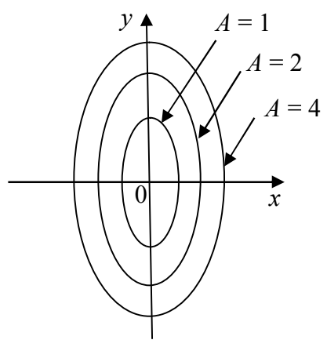
\includegraphics[width=0.3\linewidth]{images/family-soln.png}
\end{figure}
\end{solution}

\subsection{Reduction to separable form by substitution}
Some first order differential equations can be transformed by a suitable substitution into separable form.

\begin{exercise}{}{}
Find the general solution of
\[ \dv{y}{x} = \sin(x+y+1) \]
\end{exercise}

\begin{proof}[Solution]
Let $u(x) = x + y(x) + 1$ so that $\dv{u}{x} = 1 + \dv{y}{x}$. Then the original equation can be written as $\dv{u}{x} = 1 + \sin u$, which is separable. We have
\[ \frac{1}{1+\sin u}\dv{u}{x} = 1 \]
which integrates to
\[ \int \frac{1}{1+\sin u} \dd{u} = x+c \]
Let us evaluate the integral on the left hand side:
\begin{align*}
\int \frac{1}{1+\sin u} \dd{u}
&= \int \frac{1-\sin u}{(1+\sin u)(1-\sin u)} \dd{u} \\
&= \int \frac{1-\sin u}{1-\sin^2u} \dd{u} = \int \frac{1-\sin u}{\cos^2u} \dd{u} \\
&= \int \frac{1}{\cos^2u} \dd{u} - \int \frac{\sin u}{\cos^2u} \dd{u} \\
&= \tan u - \frac{1}{\cos u} + c
\end{align*}
Therefore 
\[ \tan u - \frac{1}{\cos u} = x+c \]
In terms of $x$ and $y$, the solution is given by
\[ \tan (x+y+1) - \frac{1}{\cos (x+y+1)} = x+c \]
or
\[ \sin (x+y+1) - 1 = (x+c) \cos (x+y+1). \]
This solution, where we have not found $y$ in terms of $x$, is called an \textbf{implicit solution}.
\end{proof}

A special group of first order differential equations is those of the form
\[ \dv{y}{x} = f\brac{\frac{y}{x}} \]
These differential equations are called \textbf{homogeneous} and they can be solved with a substitution
of the form
\[ y(x) = xv(x) \]
to get a new equation in terms of x and the new dependent variable $v$. This new equation will be
separable:
\[ \dv{y}{x} = v + x\dv{v}{x} \]
which becomes
\[ x\dv{v}{x} = f(v) - v \]

\subsection{Exact solutions}
LHS is an exact derivative.
\begin{exercise}{}{}
Solve 
\[ \sin x\dv{y}{x}+y\cos x=3x^2. \]
\end{exercise}
\begin{proof}[Solution]
Notice that the LHS is an exact derivative.
\begin{align*}
\sin x\dv{y}{x}+y\cos x &= \dv{x}y\sin x \\
\dv{x}y\sin x &= 3x^2 \\
y \sin x &= \int 3x^2\dd{x} = x^3+c \\
y &= \frac{x^3+c}{\sin x}
\end{align*}
\end{proof}

\subsection{Integrating Factor}
Looking specifically at first order linear ODEs, which take the general form
\[ \dv{y}{x} + P(x)y = Q(x) \]
we see that the homogeneous form, that is when $Q(x)=0$, is separable. On the other hand, the inhomogeneous form can be solved using an \textbf{integrating factor} $I(x)$ given by
\[ I(x) = e^{\int P(x) \dd{x}} \]
\begin{proof}
Simply multiply the general equation for first-order linear ODEs through by the integrating factor to obtain
\[ e^{\int P(x) \dd{x}} \dv{y}{x} + P(x) e^{\int P(x) \dd{x}}y = e^{\int P(x) \dd{x}} Q(x) \]
Using the product rule for derivatives, we see that this gives
\[ \dv{}{x}\brac{e^{\int P(x) \dd{x}}y} = e^{\int P(x) \dd{x}} Q(x) \]
and we can now integrate directly and rearrange, to obtain
\[ y = e^{-\int P(x) \dd{x}} \sqbrac{\int e^{\int P(x)dx} Q(x) \dd{x} + c}. \]
\end{proof}

\begin{exercise}{}{}
Solve the linear differential equation 
\[ \dv{y}{x} + 2xy = 2xe^{-x^2}. \]
\end{exercise}
\begin{solution}
We can easily see that the given differential equation is in the form of a first-order linear ODE.

First we find the integrating factor:
\[ I(x) = e^{\int 2x \dd{x}} = e^{x^2} \]

Multiplying the given differential equation through by the integrating factor this gives
\[ e^{x^2} \dv{y}{x} + 2xe^{x^2}y = 2x \]
that is
\[ \dv{}{x}\brac{e^{x^2}y}= 2x \]
Integrating this gives us
\[ e^{x^2}y = x^2 + c \]
so the general solution is $y = (x^2+c)e^{-x^2}$.
\end{solution}

\subsection{Qualitative approach}
\subsubsection{Slope field}


\subsubsection{Bifurcation diagram}

\subsection{Numerical methods}
\subsubsection{Euler's method}
The key principle in Euler's method is the use of a linear approximation for the tangent line to the actual solution curve $y(t)$ to approximate a solution.

Given an initial value problem
\[ \dv{y}{t}=f(t,y), \quad y(t_0)=y_0, \]
we start at $(t_0,y_0)$ on the solution curve as shown in the figure below. The equation of the tangent line through $(t_0,y_0)$ is given by
\begin{align*}
\frac{y-y_0}{t-t_0}&=f(t_0,y_0)\\
y-y_0&=(t-t_0)f(t_0,y_0)\\
y&=y_0+(t-t_0)f(t_0,y_0)
\end{align*}

\begin{figure}[H]
    \centering
    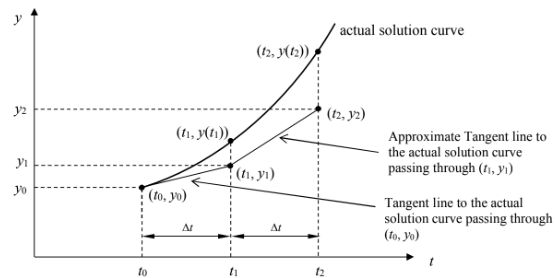
\includegraphics[width=0.75\linewidth]{images/euler-method-de.png}
\end{figure}

If we choose a step size of $\Delta t$ on the $t$-axis, then $t_1=t_0+\Delta t$. By using Euler's method, at $t=t_1$, we can obtain an approximate value $y_1$ from
\[ y_1=y_0+(t_1-t_0)f(t_0,y_0). \]
The point $(t_1,y_1)$ on the tangent line is an approximation to the point $(t_1,y(t_1))$ on the actual solution curve; that is, $y_1\approx y(t_1)$. From the figure, it is observed that the accuracy of the approximation depends heavily on the size of $\Delta t$. Hence we must choose an increment $\Delta t$ which is ``reasonably small''.

At $t=t_2$, we can similarly find the approximate valye $y_2$ from
\[ y_2=y_1+(t_2-t_1)f(t_1,y_1). \]
In general, at $t=t_{n+1}$, it follows that
\[ y_{n+1}=y_n+(t_{n+1}-t_n)f(t_n,y_n). \]
Substituting $\Delta t=t_{n+1}-t_n$, we have Euler's formula as follows:
\begin{equation}
y_{n+1}=y_n+\Delta t\cdot f(t_n,y_n)
\end{equation}
for $n=0,1,2,\dots$

\subsubsection{Improved Euler's method}
The improved Euler's method works as follows: We first apply Euler's method to find an approximation to an intermediate $y$ value and denote it as $\bar{y}_{n+1}$. We then apply Euler's method again, but now we use a linear line segment whose slope is the average of $f(t_n,y_n)$ and $f(t_{n+1},\bar{y}_{n+1})$.

\begin{figure}[H]
    \centering
    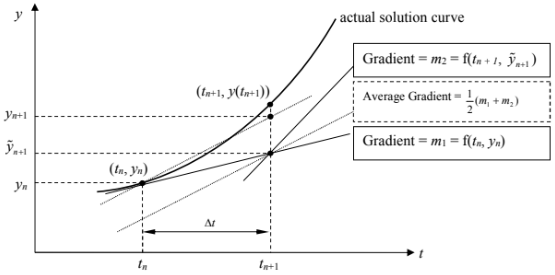
\includegraphics[width=0.75\linewidth]{images/euler-method-de-improved.png}
\end{figure}

The Improved Euler's method (also known as the Heun’s formula) consists of two steps:
\begin{equation}
\begin{split}
\bar{y}_{n+1}&=y_n+\Delta t\cdot f(t_n,y_n)\\
y_{n+1}&=y_n+\Delta t\cdot\sqbrac{\frac{f(t_n,y_n)+f(t_{n+1},\bar{y}_{n+1})}{2}}
\end{split}
\end{equation}
\pagebreak

\section{Second-order homogeneous linear ODEs}
This section introduces a method for finding a second solution to a second order homogeneous linear ODE, when one solution has already been found. Suppose $z(x)\neq0$ is a non-trivial solution to the second order homogeneous linear differential equation
\[ P(x)\dv[2]{y}{x}+Q(x)\dv{y}{x}+R(x)y=0. \]
We can make the substitution $y(x)=u(x)z(x)$, so that
\[ \dv{y}{x}=\dv{u}{x}z+u\dv{z}{x} \quad \text{and} \quad \dv[2]{y}{x}=\dv[2]{u}{x}z+2\dv{u}{x}\dv{z}{x}+u\dv[2]{z}{x}. \]
Substituting these into the above equation and using the prime to denote the derivative with respect to $x$ we obtain
\[ P(x)\brac{u^{\prime\prime}z+2u^\prime z^\prime+uz^{\prime\prime}}+Q(x)\brac{u^\prime z+uz^\prime}+R(x)uz=0. \]
If we now rearrange the above equation and use the fact that $z$ is a solution to the given equation then we get
\[ P(x)zu^{\prime\prime}+\brac{2P(x)z^\prime+Q(x)z}u^\prime=0, \]
which is a homogeneous differential equation of first order for $u^\prime$. In theory this can be solved, to obtain the general solution to the given equation. The following example illustrates this technique.

\begin{exercise}{}{}
Verify that $z(x)=\frac{1}{x}$ is a solution to
\[ x\dv[2]{y}{x}+2(1-x)\dv{y}{x}-2y=0, \]
and hence find its general solution.
\end{exercise}
\begin{solution}

\end{solution}


\todo{To edit}
\subsection{Linear with constant coefficients}
For equations in the form 
\[ a\dv[2]{y}{x} + b\dv{y}{x} +cy = 0 \]
we can write out the \textbf{auxiliary equation}
\[ am^2+bm+c=0 \]
which has roots
\[ m_{1,2}=\frac{-b\pm \sqrt{b^2-4ac}}{2a}. \]

From the nature of the roots of the auxiliary equation, we can deduce the corresponding type of general solution.
\begin{table}[H]
\centering
\begin{tabular}{c|c}
\hline\hline
\textbf{Roots of auxiliary equation} & \textbf{General solution} \\
\hline
real and distinct & $y=Ae^{m_1x}+Be^{m_2x}$ \\
real and repeated & $y=e^{mx}(A+Bx)$ \\
imaginary: $m=\alpha\pm i\beta$ & $y=e^{\alpha x}(A\cos\beta x+B\sin\beta x)$ \\
\hline\hline
\end{tabular}
\end{table}

\subsection{Non-linear}
Equation
\[ a\dv[2]{y}{x} + b\dv{y}{x} +cy = f(x) \]
where $a\neq0$, $f(x)\neq0$

General solution y=Complementary Function (CF)+Particular Integral (PI)
Complementary function: solution of the homogeneous equation

Particular integral (PI)
find by seeing different cases of f(x) and then y,dy/dx,d2y/dx2 of general PI into DE to find unknown constants of PI
If f(x) is a polynomial of degree n, $y=a_nx^n+a_{n-1}x^{n-1}+\cdots+a_1x+a_0$
When DE is a*d2y/dx2+b*dy/dx=f(x),
method 1: find CF and let PI be
\[ y=x(a_nx^n+a_{n-1}x^{n-1}+\cdots+a_1x+a_0) \]
method 2: integrate both sides wrt x and then solve accordingly

If $f(x)=qe^{kx}$ where $k$ and $q$ are constants, 

If $f(x)=k\cos ax$ or $f(x)=k\sin ax$ or $f(x)=k\cos ax+k\sin ax$

If $f(x)$ is the sum of various functions

\begin{example}[Vibrating springs]
Restoring force is given by $F=-kx$. By Newton's 2nd Law, we have $m\dv[2]{x}{t}=-kx$, or
\[ m\dv[2]{x}{t}+kx=0. \]
Hence we have auxilliary equation $mr^2+k=0$ with roots $r=\pm\omega i$ where angular frequency $\omega=\sqrt{\frac{k}{m}}$.

Thus the general solution is
\[ x(t)=c_1\cos\omega t+c_1\sin\omega t. \]
Using R-formula,
\[ x(t)=R\cos(\omega t+\delta) \]
where amplitude $R=\sqrt{c_1^2+c_2^2}$, $\cos\delta=\frac{c_1}{R}$, $\sin\delta=-\frac{c_2}{R}$, $\delta$ is known as phase angle. Period $T=\frac{2\pi}{\omega}=2\pi\sqrt{\frac{m}{k}}$.
\end{example}

\begin{example}[Damping vibrations]
Damping force is given by $F=-c\dv{x}{t}$. By Newton's 2nd law, $m\dv[2]{x}{t}=-kx-c\dv{x}{t}$, or
\[ m\dv[2]{x}{t}+c\dv{x}{t}+kx=0 \]
which has auxilliary equation $mr^2+cr+k=0$.
\begin{itemize}
\item Case 1: $c^2-4mk>0$ (over-damping)

Solution is
\[ x=c_1e^{r_1t}+c_2e^{r_2t}. \]

\item Case 2: $c^2-4mk=0$ (critical damping)

Solution is
\[ x=(c_1+c_2)e^{rt}. \]

\item Case 3: $c^2-4mk<0$ (under-damping)

Roots of auxilliary equation are $r=-\frac{c}{2m}\pm\omega i$ where $\omega=\frac{\sqrt{4mk-c^2}}{2m}$.

Solution is
\[ x=e^{-\frac{c}{2m}t}(c_1\cos\omega t+c_2\sin\omega t). \]

Amplitude follows the graph
\[ x=\pm Ae^{-\frac{c}{2m}t} \]
where $A=\sqrt{c_1^2+c_2^2}$.

For damped forced vibrations,
\[ m\dv[2]{x}{t}+c\dv{x}{t}+kx=F(t) \]
where $F(t)$ is external force.
\end{itemize}

\end{example}

\begin{example}[Electric circuits]
\[ L\dv{I}{t}+RI+\frac{Q}{C}=E \]
where $L$ is inductance, $R$ is resistance, $C$ is capacitance, $Q$ is charge, $I=\dv{Q}{t}$ is current, $E(t)$ is e.m.f.

Rewriting and taking time derivative,
\[ L\dv[2]{I}{t}+R\dv{I}{t}+\frac{1}{C}I=E^\prime(t). \]
\end{example}



Population Dynamics and Population Growth Models\todo{To look for info from F Maths notes}
• exponential growth model
• logistic growth model, equilibrium points and
their stability, and harvesting

\section{Laplace Transforms}
\subsection{Definition}
\begin{definition}
Suppose that $f(t)$ is a piecewise continuous function. The Laplace transform of $f(t)$ is denoted $\mathcal{L}\{f(t)\}$ and defined as
\begin{equation}
\mathcal{L}\{f(t)\}=\int_0^\infty e^{-st}f(t)\dd{t}.
\end{equation}
\end{definition}

\begin{notation}
For the sake of convenience we will often denote Laplace transforms as
\[ \mathcal{L}\{{f(t)}\}=F(s). \]
\end{notation}

\section{Systems of Differential Equations}
\pagebreak

\part{Calculus (Multivariable)}
\chapter{Partial Derivatives}
In multivariable calculus, we extend notions of differential calculus from functions of one variable to more general functions
\[ f:\RR^n\to\RR^m. \]

\section{Computation of partial derivatives}
Let $f:\RR^n\to\RR$ be a function of $n$ variables $x_1,x_2,\dots,x_n$. Then the \vocab{partial derivative}
\[ \pdv{f}{x_i}(p_1,\dots,p_n) \]
is the rate of change of $f$, at $(p_1,\dots,p_n)$, when we vary only the variable $x_i$ about $p_i$ and keep all of the other variables constant. Precisely, we have
\begin{equation}\label{eqn:partial-diff}
\pdv{f}{x_i}(p_1,\dots,p_n)=\lim_{h\to0}\frac{f(p_1,\dots,p_{i-1},p_i+h,p_{i+1},\dots,p_n)-f(p_1,\dots,p_n)}{h}.
\end{equation}

\begin{notation}
We shall occasionally write $f_x$ for $\delta f/\delta x$, etc.
\end{notation}

Derivatives such as \cref{eqn:partial-diff}, where $f$ has been differentiated once, are called \vocab{first order} partial derivatives. We will look at higher orders in a moment.

\begin{exercise}{}{}
Find all the first order derivatives of
\[ f(x,y,z)=x^2+ye^{2x}+\frac{z}{y}. \]
\end{exercise}

\begin{solution}
Keep in mind that we only need to find the derivative of functions with respect to one variable by keeping the rest of the variables constant.

Thus we have
\[ \pdv{f}{x}=2x+2ye^{2x}, \quad \pdv{f}{y}=e^{2x}-\frac{z}{y^2}, \quad \pdv{f}{z}=\frac{1}{y}. \]
\end{solution}

We define second and higher order partial derivatives in a similar manner to how we define them for full derivatives. So, in the case of second order partial derivatives of a function $f(x,y)$ we have
\[ \begin{split}
f_{xx} &= \pdv{}{x}\brac{\pdv{f}{x}} = \pdv[order={2}]{f}{x} \\
f_{yy} &= \pdv{}{y}\brac{\pdv{f}{y}} = \pdv[order={2}]{f}{y} \\
f_{xy} &= \pdv{}{y}\brac{\pdv{f}{x}} = \pdv{f}{x,y} \\
f_{yx} &= \pdv{}{x}\brac{\pdv{f}{y}} = \pdv{f}{y,x}
\end{split} \]

Observe that
\[ \pdv{f}{y,x}=\pdv{f}{x,y}, \quad \pdv{f}{z,x}=\pdv{f}{x,z}, \quad \pdv{f}{z,y}=\pdv{f}{y,z}. \]
This will typically be the case in the examples we will see in this course, but it is not guaranteed unless the derivatives in question are continuous.

we might have a function $f(u,v)$ of two variables $u$ and $v$, each of which is itself a function of $x$ and $y$. We can make the composition
\[ F(x,y)=f(u(x,y),v(x,y)) \]
which is a function of $x$ and $y$, and we might then want to calculate the partial derivatives
\[ \pdv{F}{x}\text{ and }\pdv{F}{y}. \]

\begin{theorem}[Chain rule]
Let $F(t)=f(u(t),v(t))$ with $u$ and $v$ differentiable and $f$ being continuously differentiable in each variable. Then
\begin{equation}
\dv{F}{t}=\pdv{f}{u}\pdv{u}{t}+\pdv{f}{v}\pdv{v}{t}
\end{equation}
\end{theorem}

\begin{corollary}
Let $F(x,y)=f(u(x,y),v(x,y))$ with $u$ and $v$ differentiable in each variable and $f$ being continuously differentiable in each variable. Then
\[ \pdv{F}{x}=\pdv{f}{u}\pdv{u}{x}+\pdv{f}{v}\pdv{v}{x}, \quad \pdv{F}{y}=\pdv{f}{u}\pdv{u}{y}+\pdv{f}{v}\pdv{v}{y}. \]
\end{corollary}

\begin{exercise}{}{}
A particle $P$ moves in three dimensional space on a helix so that at time $t$,
\[ x(t)=\cos t, \quad y(t)=\sin t, \quad z(t)=t. \]
The temperature $T$ at $(x,y,z)$ equals $xy+yz+zx$. Use the chain rule to calculate $\dv{T}{t}$.
\end{exercise}

\begin{solution}
The chain rule in this case says that
\begin{align*}
\dv{T}{t} &= \pdv{T}{x}\dv{x}{t}+\pdv{T}{y}\dv{y}{t}+\pdv{T}{z}\dv{z}{t} \\
&= (y+z)(-\sin t)+(x+z)\cos t+(y+x)(1) \\
&= (\sin t+t)(-\sin t)+(\cos t+t)\cos t+(\cos t+\sin t) \\
&= -\sin^2t+\cos^2t+\sin t+\cos t+t\cos t-t\sin t.
\end{align*}
\end{solution}

\begin{exercise}{}{}
Let $z=f(xy)$, where $f$ is an arbitrary differentiable function in one variable. Show that
\[ x\pdv{z}{x}-y\pdv{z}{y}=0. \]
\end{exercise}

\begin{solution}
By the chain rule,
\[ \pdv{z}{x}=yf^\prime(xy) \quad \text{and} \quad \pdv{z}{y}=xf^\prime(xy), \]
where the prime denotes the derivative with respect to $xy$. Hence we have
\[ x\pdv{z}{x}-y\pdv{z}{y}=xyf^\prime(xy)-yxf^\prime(xy)=0. \]
\end{solution}

\section{Directional Derivatives}
To this point we've only looked at the two partial derivatives $f_x(x,y)$ and $f_y(x,y)$. Recall that these derivatives represent the rate of change of $f$ as we vary x (holding $y$ fixed) and as we vary $y$ (holding $x$ fixed) respectively. 

We now discuss how to find the rate of change of $f$ if we allow both $x$ and $y$ to change simultaneously. The problem here is that there are many ways to allow both $x$ and $y$ to change. For instance, one could be changing faster than the other and then there is also the issue of whether or not each is increasing or decreasing. So, before we get into finding the rate of change we need to get a couple of preliminary ideas taken care of first. The main idea that we need to look at is just how are we going to define the changing of $x$ and/or $y$.

Let's start off by supposing that we wanted the rate of change of $f$ at a particular point, say $(x_0,y_0)$. Let's also suppose that both $x$ and $y$ are increasing and that, in this case, $x$ is increasing twice as fast as $y$ is increasing. So as $y$ increases one unit of measure, $x$ increases two units of measure.

Let's suppose that a particle is sitting at $(x_0,y_0)$ and the particle will move in the direction given by the changing 
$x$ and $y$. At this point, the particle can be said to be moving in the direction
\[ \vec{v} = \langle {2,1} \rangle \]

There is still a small problem with this however. There are many vectors that point in the same direction. For instance, all of the following vectors point in the same direction as $\vec v = \langle {2,1} \rangle$:
\[ \vec{v} = \left\langle {\frac{1}{5},\frac{1}{10}}\right\rangle \quad \vec{v} = \langle {6,3}\rangle \quad \vec{v} = \left\langle {\frac{2}{\sqrt{5}},\frac{1}{\sqrt{5}}}\right\rangle \]

We need a way to consistently find the rate of change of a function in a given direction. We will do this by insisting that the vector that defines the direction of change be a unit vector. This means that for the example that we started off thinking about we would want to use
\[ \vec{v} = \left\langle {\frac{2}{\sqrt{5}},\frac{1}{\sqrt{5}}}\right\rangle \]

\begin{defn}{Directional derivative}{}
Rate of change of $f(x,y)$ in the direction of the unit vector $\vec{u}=\langle{a,b}\rangle$ is called the directional derivative and is denoted by $D_{\vec{u}} f(x,y)$.

The definition of the directional derivative is
\begin{equation}
{D_{\vec u}}f(x,y) = \lim_{h\to0} \frac{f(x + ah,y + bh) - f(x,y)}{h}
\end{equation}
\end{defn}

To derive an equivalent formula for taking directional derivatives, we define a new function of a single variable
\[ g(z) = f(x_0+az,y_0+bz) \]
where $x_0$, $y_0$, $a$, $b$ are some fixed numbers. Note that this really is a function of a single variable $z$.

Then by the definition of the derivative for functions of a single variable we have
\[ g^\prime(z) = \lim_{h\to0} \frac{g(z+h)-g(z)}{h} \]
and the derivative at $z=0$ is given by
\[ g^\prime(0) = \lim_{h\to0} \frac{g(h)-g(0)}{h} \]
If we now substitute in for $g(z)$ we get
\[ g^\prime(0) = \lim_{h\to0} \frac{g(h)-g(0)}{h} = \lim_{h\to0} \frac{f(x_0+ah,y_0+bh) - f(x_0,y_0)}{h} = D_{\vec u}f(x_0,y_0) \]
This gives us
\begin{equation}\tag{1}
g^\prime(0) = D_{\vec u}f(x_0,y_0)
\end{equation}

Now, let's look at this from another perspective. Let's rewrite $g(z)$ as $g(z) = f(x,y)$ where $x=x_0+az$ and $y=y_0+bz$. Applying chain rule,
\[ g^\prime(z) = \odv{g}{z} = \pdv{f}{x}\odv{x}{z} + \pdv{f}{y}\odv{y}{z} = f_x (x,y)a + f_y (x,y)b \]
This gives us
\[ g^\prime(z) = f_x (x,y)a + f_y (x,y)b \]
If we take $z=0$ we get $x=x_0$ and $y=y_0$. Plugging these into the above equation gives
\begin{equation}\tag{2}
g^\prime(0) = f_x (x_0,y_0)a + f_y (x_0,y_0)b
\end{equation}
Equating (1) and (2) gives
\[ {D_{\vec u}}f(x_0,y_0) = f_x(x_0,y_0)a + f_y(x_0,y_0)b \]
Allowing $x$ and $y$ to be any number we get the following formula for computing directional derivatives:
\[ {D_{\vec u}}f(x,y) = f_x(x,y)a + f_y(x,y)b \]
For three variables, directional derivative of $f(x,y,z)$ in the direction of the unit vector $\vec{u}=\langle{a,b,c}\rangle$ is given by
\begin{equation}
{D_{\vec u}}f(x,y,z) = f_x (x,y,z)a + f_y (x,y,z)b + f_z (x,y,z)c
\end{equation}

We can write the directional derivative as a \textbf{dot product} and notice that the second vector is nothing more than the unit vector $\vec u$ that gives the direction of change.
\begin{equation}
{D_{\vec u}} f(x,y,z) = \langle {f_x,f_y,f_z} \rangle \cdot \langle {a,b,c} \rangle
\end{equation}

Now let's give a name and notation to the first vector in the dot product since this vector will show up fairly regularly.
\begin{defn}{Gradient vector}
The gradient vector of $f$ is defined to be
\begin{equation}
\nabla f = \langle f_x,f_y,f_z \rangle
\end{equation}
\end{defn}

With the definition of the gradient we can now say that the directional derivative is given by
\[ {D_{\vec u}}f = \nabla f\cdot \vec u \]

\begin{thrm}{}{}
Maximum value of $D_{\vec u} f(\vec{x})$ (and hence then the maximum rate of change of the function $f(\vec{x})$) is given by $\left\|\nabla f(\vec{x})\right\|$ and will occur in the direction given by $\nabla f(\vec{x})$.
\end{thrm}

\begin{proof}

\end{proof}
\pagebreak

\chapter{Partial Differential Equations}
\section{Definitions and Terminology}
\begin{definition}
A \vocab{partial differential equation} is an equation involving a function and/or its partial derivatives. 
\end{definition}

We can classify PDEs based on:
\begin{itemize}
\item \textbf{Order.}

The order is the number corresponding to the order of the highest partial derivative in the equation. 

For instance, the order of the following PDE is 2. 
\[ \pdv[order={2}]{f}{x}=\pdv{f}{t} \]

This also applies to mixed partial derivatives. For instance, the order of the following PDE is 3.
\[ \pdv[order={2,1}]{f}{x,y}=\pdv{f}{t} \]

\item \textbf{Number of independent variables.}

An independent variable is what we differentiate with respect to. 

\item \textbf{Linearity.}

A linear PDE is one in which the \emph{dependent} variable (the one being differentiated) appears only in a linear fashion.

For instance, the two PDEs above are linear as the partial derivatives are not being raised to a power or multiplied with each other.

The following PDE is non-linear.
\[ f\pdv[order={2}]{f}{x}=\pdv{f}{t} \]

\item \textbf{Homogeneity.}

A homogenous PDE is one in which every term only involves the dependent variable and/or its derivatives.

The first two PDEs above are homogenous as every term contains $f$ or its derivatives.

The following PDE is non-homogenous as there are two terms that do not contain $f$.
\[ \pdv[order={2}]{f}{x}=\pdv{f}{t}+x^2+\tan t \]

\item \textbf{Coefficient type.}

The coefficient here refers to the coefficient of the term involving the dependent variable and its derivatives. It can be either constant or variable.

For instance, the coefficients of the terms in the first two examples are 1. We say that these two PDEs have constant coefficients.

The following PDE has variable coefficients.
\[ \tan x\pdv[order={2}]{f}{x}=\pdv{f}{t} \]

\item \textbf{Parabolic, Hyperbolic, or Elliptic.}

We can do this classification for linear 2nd order PDEs which take the form of 
\[ A\pdv[order={2}]{f}{x} + B\pdv{f}{x,y} + C\pdv[order={2}]{f}{y} + D\pdv{f}{x} + E\pdv{f}{y} + Ff = G \]
where the coefficients are generally functions of $x$ or $y$.

For a \textbf{hyperbolic} PDE, $B^2-4AC>0$. Using variable substitutions to change $x$ and $y$ to $\eta$ and $\epsilon$ respectively, we can reduce the PDE to \[ \pdv[order={2}]{f}{\eta} - \pdv[order={2}]{f}{\epsilon} + g = 0 \] where $g$ denotes the first and lower order terms. This is similar to the equation of a hyperbola: $x^2-y^2=1$.

For a \textbf{parabolic} PDE, $B^2-4AC=0$. Using variable substitutions, we can reduce the PDE to \[ \pdv[order={2}]{f}{\eta} + g = 0. \] This is similar to the equation of a parabola: $x^2+y=0$.

For an \textbf{elliptic} PDE, $B^2-4AC<0$. Using variable substitutions, we can reduce the PDE to \[ \pdv[order={2}]{f}{\eta} + \pdv[order={2}]{f}{\epsilon} + g = 0. \] This is similar to the equation of an ellipse: $x^2+y^2=1$.

Note that if the coefficients are constants, the PDE can be hyperbolic, parabolic or elliptic. However, if the coefficients are variables, then it is possible for the PDE to be hyperbolic in some regions, and elliptic or parabolic in some regions.
\end{itemize}

\section{Solutions and Auxiliary Conditions}
\begin{exercise}{}{}
Show that $f(x,y)=\tan^{-1}\frac{y}{x}$ satisfies Laplace's equation in the plane:
\[ \pdv{[order={2}]}{f}{x}+\pdv{[order={2}]}{f}{y}=0. \]
\end{exercise}

\begin{solution}
The first order partial derivatives are
\[ \pdv{f}{x}=\frac{1}{1+\brac{\frac{y}{x}}^2}\brac{-\frac{y}{x^2}}=-\frac{y}{x^2+y^2} \]
and
\[ \pdv{f}{y}=\frac{1}{1+\brac{\frac{y}{x}}^2}\brac{\frac{1}{x}}=\frac{x}{x^2+y^2}. \]
Hence we have
\[ \pdv{[order={2}]}{f}{x}=\frac{2xy}{x^2+y^2} \quad \text{and} \quad \pdv{[order={2}]}{f}{y}=-\frac{2xy}{(x^2+y^2)^2}, \]
from which we see that
\[ \pdv{[order={2}]}{f}{x}+\pdv{[order={2}]}{f}{y}=0 \]
as required.
\end{solution}

In the above example we verified that a given solution satisfied a given PDE. We now look at how to find solutions to simple PDEs.

\begin{exercise}{}{}
Find all the solutions of the form $f(x,y)$ of the PDEs
\begin{enumerate}[label=(\alph*)]
\item $\pdv{f}{y,x}=0$,
\item $\pdv{[order={2}]}{f}{x}=0$.
\end{enumerate}
\end{exercise}

\begin{solution} \
\begin{enumerate}[label=(\alph*)]
\item We have
\[ \pdv{}{y}\brac{\pdv{f}{x}}=0. \]
Those functions $g(x,y)$  which satisfy $\delta g/\delta y=0$ are functions which solely depend on $x$. So we have
\[ \pdv{f}{x}=p(x), \]
where $p$ is an arbitrary function of $x$. We can now integrate again, but this time with respect to $x$ rather than $y$. Now, $\delta/\delta x$ sends to zero any function which solely depends on $y$. The solution to the PDE is therefore
\[ f(x,y)=P(x)+Q(y), \]
where $Q(y)$ is an arbitrary function of $y$ and $P(x)$ is an anti-derivative of $p(x)$, i.e. $P^\prime(x)=p(x)$.
\end{enumerate}
\end{solution}

If a PDE involves derivatives with respect to one variable only, we can treat it like an ODE in that variable, holding all other variables constant. The difference, as noted above, is that our arbitrary ``constants'' will now be arbitrary functions of the variables that we have held constant.

\begin{exercise}{}{}
Find solutions $u(x,y)$ of the PDE
\[ u_{xx}-u=0. \]
\end{exercise}

\begin{solution}
Since there are no derivatives with respect to $y$, we can solve the associated ODE
\[ \dv[2]{u}{x}-u=0, \]
where $u$ is treated as being a function of $x$ only. This ODE has solution $u(x)=C_1e^x+C_2e^{-x}$, where $C_1$ and $C_2$ are constants, and so the solution to the original PDE is
\[ u(x,y)=A(y)e^x+B(y)e^{-x}, \]
where $A$ and $B$ are arbitrary functions of $y$ only.
\end{solution}

we look at one specific method for solving PDEs, that of \textbf{separating the variables}.

\begin{exercise}{}{}
Find all solutions of the form $T(x,t)=A(x)B(t)$ to the one-dimensional heat/diffusion equation
\[ \pdv{T}{t}=\kappa\pdv{[order={2}]}{T}{x}, \]
where $\kappa$ is a positive constant, called the thermal diffusivity.
\end{exercise}

Solutions of the form $A(x)B(t)$ are known as separable solutions

There are a lot of solutions to a given PDE, hence it is important for us to know the auxiliary conditions, i.e. boundary and initial conditions, which dictate which technique we use to solve the PDE.
\begin{itemize}
\item A boundary condition expresses the behavior of a function on the boundary (border) of its area of definition. An initial condition is like a boundary condition, but then for the time-direction.
\end{itemize}
\pagebreak

\chapter{Multiple Integrals}
\section{Double Integrals}
To motivate the idea of double integrals, we give an example of calculating areas.

We want to integrate a function of two variables, $f(x,y)$. With functions of one variable we integrated over an \emph{interval} (i.e. a one-dimensional space) and so it makes some sense then that when integrating a function of two variables we will integrate over a \emph{region} of $\RR^2$ (two-dimensional space). 

\begin{exercise}{}{}
Calculate the area of the disc $x^2+y^2\le a^2$.
\end{exercise}

\begin{solution}
we know the answer, namely $\pi a^2$. If we wish to capture all of the disc's area then we let $x$ vary from $-a$ to $a$ and, at each $x$ we let $y$ vary from $-\sqrt{a^2-x^2}$ to $\sqrt{a^2-x^2}$.

Thus we have
\begin{align*}
A &= \int_{x=-a}^{x=a}\int_{y=-\sqrt{a^2-x^2}}^{y=\sqrt{a^2-x^2}}\dd{y}\dd{x} \\
&= \int_{x=-a}^{x=a}2\sqrt{a^2-x^2}\dd{x} \\
&= \int_{\theta=-\frac{\pi}{2}}^{\theta=\frac{\pi}{2}}2\sqrt{a^2-a^2\sin^2\theta}a\cos\theta\dd{\theta} \quad [x=a\sin\theta] \\
&= a^2\int_{\theta=-\frac{\pi}{2}}^{\theta=\frac{\pi}{2}}2\cos^2\theta\dd{\theta}=\pi a^2
\end{align*}
\end{solution}

\begin{definition}
Let $R\subset\RR^2$. Then we define the \vocab{area} of $R$ to be
\[ A(R)=\iint_{(x,y)\in R}\dd{x}\dd{y}. \]
\end{definition}

% https://tutorial.math.lamar.edu/classes/calciii/DoubleIntegrals.aspx

Recall that given a function $f(x)$, the definite integral $\int_a^bf(x)\dd{x}$ evaluates the area under the curve $y=f(x)$ between $x=a$ and $x=b$. Similarly given a function $f(x,y)$, the volume of the solid below the graph $z=f(x,y)$ and above the region $R$ in the $xy$-plane is given by 
\begin{equation}
V=\iint_Rf(x,y)\dd{A}.
\end{equation}

\begin{remark}
You can think of $\iint$ as a sum of heights $f(x,y)$ and areas $\dd{A}$, which evaluates to give a volume.
\end{remark}

\begin{exercise}{}{}
Let $R$ be the triangle whose vertices are $(0,0,0)$, $(0,1,0)$ and $(1,0,0)$. Evaluate $\iint_R1\dd{A}$.
\end{exercise}

\begin{solution}
$\iint_R1\dd{A}$ is the volume of a prism with height $1$ and base of area $R$. Hence
\[ \iint_R1\dd{A}=\text{Area of }R\times1=\frac{1}{2}\times1\times1\times1=\boxed{\frac{1}{2}} \]
\end{solution}

To evaluate double integrals we need a notion called iterated integrals, which are basically two integrals with one nested inside the other.

\begin{exercise}{}{}
Evaluate 
\begin{enumerate}[label=(\alph*)]
\item $\displaystyle\int_0^1\int_1^2x+2y\dd{x}\dd{y}$
\item $\displaystyle\int_{-1}^1\int_0^x3x^2+2y\dd{y}\dd{x}$
\end{enumerate}
\end{exercise}

\begin{solution}
\begin{enumerate}[label=(\alph*)]
\item 
\begin{align*}
\int_0^1\int_1^2x+2y\dd{x}\dd{y}
&= \int_0^1\brac{\int_1^2x+2y\dd{x}}\dd{y} \\
&= \int_0^1\sqbrac{\frac{x^2}{2}+2yx}_{x=1}^{x=2}\dd{y} \\
&= \int_0^12y+\frac{3}{2}\dd{y} \\
&= \sqbrac{y^2+\frac{3}{2}y}_{y=0}^{y=1}=\boxed{\frac{5}{2}}
\end{align*}

\item 
\begin{align*}
\int_{-1}^1\int_0^x3x^2+2y\dd{y}\dd{x}
&= \int_{-1}^1\brac{\int_0^x3x^2+2y\dd{y}}\dd{x} \\
&= \int_{-1}^1\sqbrac{3x^2y+y^2}_{y=0}^{y=x}\dd{x} \\
&= \int_{-1}^13x^3+x^2\dd{x} \\
&= \sqbrac{\frac{3x^4}{4}+\frac{x^3}{3}}_{x=-1}^{x=1}=\boxed{\frac{2}{3}}
\end{align*}
\end{enumerate}
\end{solution}

\section{Iterated Integrals}
Now we are going to discuss the relation between double integrals and iterated integrals.

$R$ is called simple if $R$ is a rectangle given by $a\le x\le b$ and $c\le y\le d$, in which case
\[ \iint_Rf(x,y)\dd{A}=\int_a^b\int_c^df(x,y)\dd{y}\dd{x}=\int_c^d\int_a^bf(x,y)\dd{x}\dd{y}. \]
This is known as Fubini's Theorem.

$R$ is called vertically simple if $R$ is given by $a\le x\le b$, $g(x)\le y\le h(x)$, in which case
\[ \iint_Rf(x,y)\dd{A}=\int_a^b\int_{g(x)}^{h(x)}f(x,y)\dd{y}\dd{x}. \]

$R$ is called horizontally simple if $R$ is given by $c\le y\le d$, $g(y)\le x\le h(y)$, in which case
\[ \iint_Rf(x,y)\dd{A}=\int_c^d\int_{g(y)}^{h(y)}f(x,y)\dd{x}\dd{y}. \]

% https://tutorial.math.lamar.edu/Classes/CalcIII/DIGeneralRegion.aspx
\pagebreak

\chapter{Line Integrals}
\section{Vector fields}
A vector field is basically what you get when associating each point in space with a vector.

\begin{definition}
A \vocab{vector field} on two (or three) dimensional space is a function $\vec{F}$ that assigns eahc point $(x,y)$ (or $(x,y,z)$) a two (or three) dimensional vector given by $\vec{F}(x,y)$ (or $\vec{F}(x,y,z)$).
\end{definition}

The standard notation for the function $\vec{F}$ is:
\begin{align*}
\vec{F}(x,y) &= P(x,y)\hat{i} + Q(x,y)\hat{j} \\
\vec{F}(x,y,z) &= P(x,y,z)\hat{i} + Q(x,y,z)\hat{j} + R(x,y,z)\hat{k}
\end{align*}
depending on whether or not we're in two or three dimensions. The functions $P$, $Q$, $R$ are called \textbf{scalar functions}.

\begin{exercise}{}{}
Sketch the following vector field:
\[ \vec{F}(x,y) = -y\hat{i} + x\hat{j} \]
\end{exercise}
\begin{solution}
To graph the vector field we need to get some ``values'' of the function. This means plugging in some points into the function. Here are a couple of evaluations:
\begin{align*}
\vec{F}\brac{{\frac{1}{2},\frac{1}{2}}} &=  -\frac{1}{2}\hat{i} + \frac{1}{2}\hat{j} \\
\vec{F}\brac{{\frac{1}{2},-\frac{1}{2}}} &=  -\brac{{-\frac{1}{2}}}\hat{i} + \frac{1}{2}\hat{j} = \frac{1}{2}\hat{i} + \frac{1}{2}\hat{j} \\
\vec{F}\brac{{\frac{3}{2},\frac{1}{4}}} &=  -\frac{1}{4}\hat{i} + \frac{3}{2}\hat{j}
\end{align*}
So what do these evaluations tell us? The first one tells us that at the point $\brac{\dfrac{1}{2},\dfrac{1}{2}}$ we plot the vector $-\frac{1}{2}\hat{i} + \frac{1}{2}\hat{j}$.

Plotting points gives us the following sketch of the vector field:

\begin{figure}[H]
    \centering
    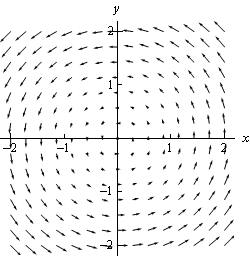
\includegraphics[width=8cm]{images/vec_field2.png}
\end{figure}
\end{solution}

Recall that given a function $f(x,y,z)$ the gradient vector is defined as such:
\begin{definition}
Given a function $f(x,y,z)$, the gradient vector is defined by
\[ \nabla f\coloneqq\left\langle {{f_x},{f_y},{f_z}} \right\rangle. \]
This is a vector field and is often called a \vocab{gradient vector field}.
\end{definition}

\section{Types of line integrals}

\section{Fundamental Theorem for Line Integrals}
\begin{thrm}{Fundamental Theorem of Line Integrals}{}
Suppose that $C$ is a smooth curve from points $A$ to $B$ parameterised by $\vb{r}(t)$ for $t\in[a,b]$. Let $f$ be a differentiable function whose domain includes $C$ and whose gradient vector $\nabla f$ is continuous on $C$. Then
\begin{equation}
\int_C \nabla f \dd{\vb{r}} = f(\vb{r}(b)) - f(\vb{r}(a)) = f(B) - f(A)
\end{equation}
\end{thrm}
\begin{remark}
Similar to the fundamental theorem of calculus, the primary change is that gradient $\nabla f$ takes the place of the derivative $f^\prime$.
\end{remark}
% https://www.math.uci.edu/~ndonalds/math2e/16-3fundthm.pdf
% https://www.youtube.com/watch?v=_60sKaoRmhU

\section{Conservative Vector Fields}

\section{Green's Theorem}


to compute arc lengths, areas of curves 

applications of integrals to find area and volume

\chapter{Surface Integrals}


\part{Differential Geometry}
\textbf{Readings:}
\begin{itemize}
\item \href{https://aetemad.iut.ac.ir/sites/aetemad.iut.ac.ir/files/files_course/william_m._boothby_an_introduction_to_differentibookfi.org_.pdf}{Introduction to Differentiable Manifolds and Riemannian Geometry}
\item \href{http://www2.ing.unipi.it/griff/files/dC.pdf}{Differential Geometry of Curves and Surfaces}
\end{itemize}
\part{Complex Analysis}
\chapter{Complex Numbers}
\section{The Algebra of Complex Numbers}
\subsection{Arithmetic Operations}
\vocab{Imaginary unit} $i=\sqrt{-1}$. A \vocab{complex number} $z=\alpha+i\beta$ where $\alpha,\beta\in\RR$; $\alpha$ and $\beta$ are the real and imaginary parts of the complex number respectively. If $\alpha=0$, the number is said to be purely imaginary; if $\beta=0$, it is real. Zero is the only number which is at once real and purely imaginary.

Two complex numbers are equal if and only if they have the same real part and the same imaginary part.

Addition and multiplication do not lead out from the system of complex numbers. Assuming that the ordinary rules of arithmetic apply to complex numbers we find indeed
\[(\alpha+i\beta)+(\gamma+i\delta)=(\alpha+\gamma)+i(\beta+\delta)\]
and
\[(\alpha+i\beta)(\gamma+i\delta)=(\alpha\gamma-\beta\delta)+i(\alpha\delta+\beta\gamma),\]
making use of the relation $i^2=-1$.

It is less obvious that division is also possible. We wish to show that $\dfrac{\alpha+i\beta}{\gamma+i\delta}$ is a complex number, provided that $\gamma+i\delta\neq0$. Denoting the quotient by $x+iy$, we have
\begin{align*}
\alpha+i\beta&=(\gamma+i\delta)(x+iy)\\
&=
\end{align*}

\subsection{Square Roots}
\subsection{Justification}
\subsection{Conjugation, Absolute Value}
\subsection{Inequalities}
%\part{Harmonic Analysis}
\chapter{Fourier Analysis}
While developing the theory of heat conduction in the early 19th century, Jean--Baptiste Joseph Fourier kick-started a mathematical revolution by claiming that ``every'' real-valued function defined on a finite interval could be expanded as an infinite series of elementary trigonometric functions -- cosines and sines.

\section{Fourier Series}
Given a function $f:\RR\to\RR$ that is periodic with period $2\pi$, Fourier's claim is equivalent to the assertion that there exists constants $a_0,a_1,\dots$ and $b_1,b_2,\dots$ in terms of which $f$ may be expanded in the form
\begin{equation}\label{eqn:fourier-series}
f(x)=\frac{a_0}{2}+\sum_{n=1}^\infty\brac{a_n\cos nx+b_n\sin nx} \text{ for } x\in\RR
\end{equation}
the infinite series on the RHS being the \vocab{Fourier series} for $f$.

\begin{remark}
In later sections it will become apparent that the choice to focus on functions of period $2\pi$ and the factor of $\frac{1}{2}$ in the leading term in \cref{eqn:fourier-series} are both for algebraic convenience.
\end{remark}

\subsection{Periodic, even and odd functions}
The building blocks that form the partial sums of a Fourier series are cosines and sines. Not only are cosines and sines infinitely differentiable on $\RR$, their graphs have important periodicity and symmetry properties: $\cos$ is an even periodic function, while $\sin$ is an odd periodic function. We therefore start with a refresher of what it means for a function to have these properties.

\begin{definition}
The function $f:\RR\to\RR$ is a \vocab{periodic function} if there exists $p>0$ such that
\[ f(x+p)=f(x) \quad \text{for all }x\in\RR. \]
In this case $p$ is a \vocab{period} for $f$ and $f$ is called \vocab{$p$-periodic}. A period is not unique, but if there exists a smallest such $p$ it is called the \vocab{prime period}.
\end{definition}

If a function is defined on a half-open interval of length $p>0$, i.e. on $(\alpha,\alpha+p]$ or $[\alpha,\alpha+p)$ for some $\alpha\in\RR$, then we can extend it to a unique periodic function by demanding it to be periodic with period $p$. Formally, we define as follows the periodic extension of such a function.

\begin{definition}
The \vocab{periodic extension} of the function $f:(\alpha,\alpha+p]\to\RR$ is the function $F:\RR\to\RR$ defined by
\[ F(x) = f\brac{x-m(x)p} \quad \text{for }x\in\RR \]
where, for each $x\in\RR$, $m(x)$ is the unique integer such that $x-m(x)p\in(\alpha,\alpha+p]$.
\end{definition}

\begin{definition}
The function $g:\RR\to\RR$ is \vocab{even} if $g(x)=g(-x)$ for all $x\in\RR$.
\end{definition}

\begin{definition}
The function $h:\RR\to\RR$ is \vocab{odd} if $h(x)=-h(-x)$ for all $x\in\RR$.
\end{definition}

\begin{proposition}
Given a function $f:\RR\to\RR$ there exist unique functions $g:\RR\to\RR$ and $h:\RR\to\RR$ with $g$ even and $h$ odd such that $f(x)=g(x)+h(x)$ for $x\in\RR$.
\end{proposition}

\begin{proof}
To prove existence note that the following functions have the required properties:
\[ g(x)=\frac{1}{2}\brac{f(x)+f(-x)}, \quad h(x)=\frac{1}{2}\brac{f(x)-f(-x)} \quad \text{for }x\in\RR. \]
To prove uniqueness suppose that $f=g_1+h_1$ and $f=g_2+h_2$, with $g_1,g_2$ even and $h_1,h_2$ odd; then $g_1-g_2=h_2-h_1$ is both even and odd, and hence must vanish on $\RR$.
\end{proof}

\subsection{Fourier series for functions of period $2\pi$}
Suppose \cref{eqn:fourier-series} is true and that we can integrate it term-by-term over a period, so that
\[ \int_{-\pi}^\pi f(x)\dd{x}=\frac{a_0}{2}\int_{-\pi}^\pi\dd{x}+\sum_{n=1}^\infty\brac{a_n\int_{-\pi}^\pi\cos nx\dd{x}+b_n\int_{-\pi}^\pi\sin nx\dd{x}}. \]
Since, for positive integers $n$,
\[ \int_{-\pi}^\pi\dd{x}=2\pi, \quad \int_{-\pi}^\pi\cos nx\dd{x}=0, \quad \int_{-\pi}^\pi\sin nx\dd{x}=0, \]
we must have
\begin{equation}\label{eqn:fourier-leading}
a_0=\frac{1}{\pi}\int_{-\pi}^\pi f(x)\dd{x}
\end{equation}
which determines $a_0$ in terms of $f$.

\begin{remark}
Since $f$ is $2\pi$-periodic we could have integrated over any interval of length $2\pi$.
\end{remark}

\begin{remark}
The leading term $\frac{a_0}{2}$ in the Fourier series \cref{eqn:fourier-leading} is equal to the mean of $f$ over a period.
\end{remark}

In order to determine the higher-order Fourier coefficients we will need the following lemma.

\begin{lemma}
Let $m$ and $n$ be positive integers. Then we have the orthogonality relations:

\end{lemma}

% https://courses.maths.ox.ac.uk/pluginfile.php/93584/mod_resource/content/1/FSPDE-Lectures-Notes.pdf

\subsection{Cosine and sine series}
\subsection{Tips for evaluating the Fourier coefficients}
\subsection{Convergence of Fourier series}
\subsection{Rate of convergence}
\subsection{Gibb's phenomenon}
\subsection{Functions of any period}
\subsection{Half-range series}


%\part{Discrete Mathematics}
\chapter{Graph Theory}
% Clear this first: https://web.evanchen.cc/notes/SJSU179.pdf
% https://web.mit.edu/yufeiz/www/imo2008/tang-graph.pdf
% https://yufeizhao.com/211/graph_theory_notes.pdf
% https://courses.maths.ox.ac.uk/pluginfile.php/29835/mod_resource/content/2/GraphTheoryPartA-notes-2023.pdf

\section{Definitions}
\subsection{Preliminary Definitions}
\begin{definition}
A \vocab{graph} $G = (V(G),E(G))$ consists of two sets $V(G)$ (the \vocab{vertex} set) and $E(G)$ (the \vocab{edge} set), where each element of $E(G)$ consists of a pair of elements of $V(G)$. 
\end{definition}

\begin{notation}
$|G|=|V(G)|$ denotes the number of vertices and $e(G) =|E(G)|$ denotes the number of edges.
\end{notation}

The \vocab{order} of a graph $G$ is $|V(G)|$. The \vocab{size} of $G$ is $|E(G)|$.

We represent $G$ visually by drawing a point for each vertex and a line between any pair of points that form an edge.

The \vocab{complement} of $G$, denoted by $\overline{G}$, is a graph with the same vertex set as $G$ and $E(\overline{G}) = \{e \notin E(G)\}$, i.e. $\overline{G}$ has edges exactly where there are no edges in $G$.

\begin{definition}
A loop is an edge $(v,v)$ for some $v \in V$. An edge $e=(u,v)$ is a multiple edge if it appears multiple times in $E$. 

A graph is \vocab{simple} if it has no loops or multiple edges.
\end{definition}

\begin{remark}
Unless explicitly stated otherwise, we will only consider simple graphs. General (potentially non-simple) graphs are also called multigraphs.
\end{remark}

Vertices $u$ and $v$ are \vocab{neighbours} if $(u,v) \in E(G)$; we also say that $u$ and $v$ are \vocab{adjacent}. An edge $e \in E(G)$ is \vocab{incident} to a vertex $v \in V(G)$ if $v \in e$. Edges $e, e^\prime$ are \vocab{incident} if $e \cap e^\prime = \emptyset$.

Given a vertex $v$, the \vocab{degree} of $v$, denoted by $d(v)$, is the number of neighbours of $v$ in $G$. If the degree of each vertex is the same, we can call that the degree of the graph. A \vocab{leaf} is a vertex of degree one, i.e. with a unique neighbour.

\begin{remark}
A trivial graph is a graph with order 1. An empty graph is a graph of size 0. 
Note that a graph must have at least one vertex by definition. But a graph can certainly have no edges!
\end{remark}

\subsection{Subgraph}
\begin{definition}
$H$ is a \vocab{subgraph} of $G$ if $V(H) \subseteq V(G)$ and $E(H) \subseteq E(G)$.
\end{definition}

$H$ is a \vocab{spanning subgraph} if $V(H)=V(G)$.

$H$ is an \vocab{induced subgraph} if $(u,v) \in E(H) \iff (u,v) \in E(G) \forall u, v \in V(H)$.

\subsection{Walks}
\begin{definition}
A \vocab{$u-v$ walk} in $G$, denoted by $W$, is a finite sequence of vertices $u=v_0,v_1,\dots,v_k=v$ such that $v_i v_{i+1} \in E(G)$ for all $0 \le i < k-1$.
\end{definition}

A walk is \vocab{closed} if and only if $u=v$. Otherwise, it is \vocab{open}.

A \vocab{trail} is an open walk without repeating vertices.

A \vocab{path} is an open walk without repeating edges.
Note that paths are trails, but not vice-versa.

A \vocab{circuit} is a closed walk without repeating edges, i.e. $u=v$, it begins and ends with the same vertex.

A \vocab{cycle} is a closed walk without repeating vertices, other than the initial and terminal vertices, i.e. $u=v$ but the vertices are otherwise distinct and $W$ has at least 3 vertices. If a graph $G$ has no cycle we call it \vocab{acyclic}.

A \vocab{trail} is a walk in which no two vertices appear consecutively (in either order) more than once; that is, no edge is used more than once. A \vocab{tour} is a closed trail.

\subsection{Connectedness}
\begin{definition}
A graph $G$ is \vocab{connected} if $\forall u,v \in V(G)$ there exists a $u-v$ path.
\end{definition}

Let $G$ be a connected graph. Then $d(u,v)$ is the \vocab{smallest length} of any $u-v$ path if $u \neq v$, or 0 if $u=v$.

The \vocab{diameter} of a connected graph $G$, denoted by $\diam G$, is defined as
\[ \diam G = \max_{u\neq v} d(u,v). \]
By construction, $d(u,v) \le \diam G \forall u,v \in V(G)$.

We say that two vertices $u$ and $v$ of a graph $G$ lie in the same \vocab{component} if they are joined by an $u-v$ walk. Clearly this forms an equivalence relation and the partition of $V(G)$ into equivalence classes expresses $G$ as a union of disjoint connected graphs called its components.

$G$ is \vocab{complete} if every pair of vertices in $G$ is joined by an edge. A complete graph on $n$ vertices is denoted by $K_n$.

\subsection{Classes of graphs}
\vocab{Empty graph}: We let $E_n$ denote the empty graph with order $n$ and size 0. This graph is disconnected if and only if $n \ge 2$.

\vocab{Path graph}: We let $P_n$ be the graph of order $n$ and size $n-1$. You can guess what this is: It is connected with diameter $n-1$.

\vocab{Cycle graph}: We let $C_n$ denote the graph of order $n$ and size $n$ which consists of a single
cycle. Note that $n \ge 3$. It is connected with diameter $\floor{\frac{1}{2}n}$.

\vocab{Complete graph}: We let $K_n$ denote the complete graph, with order $r$ and size $\binom{n}{2}$. It is extremely connected with diameter 1 (for $n \ge 2$). Note that this is the only class of connected graphs with diameter 1.

Note that $E_1 = K_1 = P_1$, $K_2 = P_2$ and $K_3 = C_3$.

\subsection{Bipartite Graphs}
$G$ is \vocab{bipartite} if $V(G)$ can be partitioned into two non-empty disjoint sets $A$ and $B$ such that no edge has both endpoints in the same set. A graph is said to be \vocab{complete bipartite} if $G$ is bipartite and all possible edges between the two sets $A$ and $B$ are drawn. In the case where $|A|=m, |B|=n$, such a graph is denoted by $K_{m,n}$.

Let $k \ge 2$. A graph $G$ is said to be \vocab{$k$-partite} if $V(G)$ can be partitioned into $k$ pairwise disjoint sets $A_1, \dots, A_k$ such that no edge has both endpoints in the same set. A \vocab{complete $k$-partite} graph is defined similarly as a complete bipartite. In the case where $|A_i| = n_i$, such a graph is denoted by $K_{n_1,n_2,\dots,n_k}$.

A graph is \vocab{planar} if it can be drawn such that a pair of edges can only cross at a vertex.

\begin{thrm}{Euler's Characteristic Formula}{}
For any connected planar graph, the number of vertices $V$ minus the number of edges $E$ plus the number of regions $R$ equals 2. 
\begin{equation} V-E+R = 2 \end{equation}
\end{thrm}

(or V-E+F=2 for 3 dimensional polyhedra)
To prove this, 
for trivial graph, V=1, F=1, E=0
Adding one edge, we either introduce a new vertex or face (if edge is connected to preexisting vertex)



\subsection{Isomorphism}
\begin{defn}{Isomorphism}{}
Let $G_1 = (V_1, E_1)$ and $G_2 = (V_2, E_2)$ be graphs. An isomorphism $\phi : G_1 \to G_2$ is a bijection (a one-to-one correspondence) from $V_1$ to $V_2$ such that $(u,v) \in E_1$ if and only if $(\phi(u),\phi(v)) \in E_2$. We say $G_1$ is isomorphic to $G_2$ if there is an isomorphism between them.
\end{defn}



\section{Trees and Balancing}
A \vocab{tree} is defined to be a connected graph that does not contain any cycles; to put it simply, it is a minimally connected graph.

A \vocab{cycle} in a graph means there is a path from an object back to itself.

Characterisation of trees: Let $G$ be a connected graph with $n$ vertices. The following statements are equivalent.
\begin{enumerate}
\item $G$ does not contain any cycles
\item $G$ contains exactly $n-1$ edges
\item For any two vertices, there exists exactly one path joining the two vertices
\item The removal of any edge disconnects the graph
\end{enumerate}

\begin{lemma}\label{acyclic}
Any tree is acyclic.
\end{lemma}
\begin{proof}
Let $G$ be a tree, i.e. $G$ is minimally connected. Suppose for a contradiction that $G$ contains a cycle $C$. Let $e \in E(C)$. We will obtain our contradiction by showing that $G-e \coloneqq (V(G),E(G)\setminus\{e\})$ is connected. 

Let $P$ be the path obtained by deleting $e$ from $C$. Consider any $u,v$ in $V(G)$. As $G$ is connected, there is an $u-v$ walk $W$ in $G$. Replacing any use of $e$ in $W$ by $P$ gives an $u-v$ walk in $G-e$. Thus $G-e$ is connected, a contradiction.
\end{proof}

There are many equivalent characterisations of trees, any of which could be taken as the definition. Here is one:

\begin{lemma}\label{tree_iff}
$G$ is a tree if and only if $G$ is connected and acyclic.
\end{lemma}
\begin{proof}
If $G$ is a tree then $G$ is connected by definition and acyclic by \cref{acyclic}. Conversely, let $G$ be connected and acyclic. Suppose for a contradiction that $G-e$ is connected for some $e = (u,v) \in E(G)$.

Let $W$ be a shortest $u-v$ walk in $G-e$. Then $W$ must be a path, i.e. have no repeated vertices, otherwise we would find a shorter walk by deleting a segment of $W$ between two visits to the same vertex. Combining $W$ with $(u,v)$ gives a cycle, which is a contradiction.
\end{proof}

\begin{remark}
The fact that a shortest walk between two points is a path is often useful. More generally, considering an extremal (shortest, longest, minimal, maximal, \dots) object is often a useful proof technique.
\end{remark}

\begin{lemma}
Any two vertices in a tree are joined by a unique path.
\end{lemma}
\begin{proof}
Suppose for a contradiction that this fails for some tree $G$. 

Choose $u,v$ in $V(G)$ so that there are distinct $u-v$ paths P1, P2, and P1 is as short as possible over all such choices of $u$ and $v$.

Then P1 and P2 only intersect in $u$ and $v$, so their union is a cycle, contradicting \cref{acyclic}.
\end{proof}

\begin{lemma}\label{tree_leaves}
Any tree with at least two vertices has at least two leaves.
\end{lemma}
\begin{proof}
Consider any tree $G$. Let $P$ be a longest path in $G$. The two ends of $P$ must be leaves. Indeed, an end cannot have a neighbour in $V(G) \setminus V(P)$, or we could make $P$ longer, and cannot have any neighbour in $V(P)$ other than the next in the sequence of $P$, or we would have a cycle.

The existence of leaves in trees is useful for inductive arguments, via the following lemma. Given $v \in V(G)$, let $G-v$ be the graph with $V(G-v) = V(G)\setminus\{v\}$ and $E(G-v) = \{(u,v) \in E(G) \mid v \notin \{u,v\}\}$.
\end{proof}

\begin{lemma}\label{tree_leaf}
If $G$ is a tree and $v$ is a leaf of $G$ then $G-v$ is a tree.
\end{lemma}
\begin{proof}
By \cref{tree_iff} it suffices to show that $G-v$ is connected and acyclic. Acyclicity is immediate from \cref{acyclic}. Connectedness follows by noting for any $u,v \in V(G)\setminus\{v\}$ that the unique $u-v$ path in $G$ is contained in $G-v$.
\end{proof}

\begin{lemma}\label{tree_edges}
Any tree on $n$ vertices has $n-1$ edges.
\end{lemma}
\begin{proof}
By induction. A tree with 1 vertex has 0 edges. Let $G$ be a tree on $n>1$ vertices. By \cref{tree_leaves}, $G$ has a leaf $v$. By \cref{tree_leaf}, $G-v$ is a tree. By induction hypothesis, $G-v$ has $n-2$ edges. Replacing $v$ gives $n-1$ edges in $G$.
\end{proof}

We conclude this section with another characterisation of trees. First we note that any connected graph $G$ contains a minimally connected subgraph (i.e. a tree) with the same vertex set, which we call a \vocab{spanning tree} of $G$.

\begin{lemma}
A graph $G$ is a tree on $n$ vertices if and only if $G$ is connected and has $n-1$ edges.
\end{lemma}
\begin{proof}
If $G$ is a tree then $G$ is connected by definition and has $n-1$ edges by \cref{tree_edges}. 

Conversely, suppose that $G$ is connected and has $n-1$ edges. Let $H$ be a spanning tree of $G$. Then $H$ has $n-1$ edges by \cref{tree_edges}, so $H = G$, so $G$ is a tree.
\end{proof}

\section{Euler Tours and Trails}
An \vocab{Euler trail} is a trail in which every pair of adjacent vertices appear consecutively. (That is, every edge is used exactly once.)

An \vocab{Euler tour} is a closed Euler trail.


vertex/edge colouring and Ramsey Theory

Regular graph
Directed graph

graph concepts such as Shortest-, Euler-, Hamilton-Paths and Cycles, coloring, planarity, weighted graphs, and directed graphs.

Topics in graph theory, including: connectivity and matchings, Hall's theorem, Menger's theorem, network flows; paths and cycles, complete subgraphs and Turán's theorem, and the Erdös-Stone theorem; graph colouring and the four-colour theorem; Ramsey theory; probabilistic methods in graph theory; and the use of software to solve graph-theoretic problems.
\pagebreak

\section*{Problems}
\begin{prbm}[K\"{o}nigsberg Bridge Problem]
K\"{o}nigsberg was a small town in Prussia. There is a river running through the town and there were seven bridges across the river. The inhabitants of K\"{o}nigsberg liked to walk around the town and cross all of the bridges:

Is it possible to walk around the town and cross every bridge, once and once only?
\end{prbm}

\begin{solution}
We replace every landmass by a vertex and every bridge by an edge to give the following graph.


\end{solution}
\pagebreak

Problems can include tournament, matching, and scheduling problems.
\begin{prbm}(Moser's circle problem) 
Determine the number of regions into which a circle is divided if $n$ points on its circumference are joined by chords with no three internally concurrent.
\end{prbm}

\begin{proof}[Solution]
Consider the graph which has points on the circumference and intersection points between chords as its vertices.

Let $V, E, F$ denote the number of vertices, edges, regions respectively.

To count the number of intersection points, note that $4$ points on the circumference give one unique intersection point between the two non-parallel chords formed by connecting two pairs of points which intersect inside the circle. Hence, number of intersection points is $\dbinom{n}{4}$. 
\[ V = n + \binom{n}{4} \]
Total number of edges includes $n$ circular arcs, number of original chords formed from connecting pairs of points on the circumference
E = no. of original lines + 2 x no. of intersection points
E = n choose 2 + 2 x n choose 4 + n
since there are n circular arcs

Using Euler's Characteristic Formula, we have 
\begin{align*}
F &= E - V - 1 \\
\Aboxed{F &= 1 + \binom{n}{2} + \binom{n}{4}}
\end{align*}
\end{proof}

\chapter{Game Theory}
\textbf{Recommended readings:} \href{https://mathematicalolympiads.files.wordpress.com/2012/08/martin_j-_osborne-an_introduction_to_game_theory-oxford_university_press_usa2003.pdf}{``An Introduction to Game Theory" by Osborne}

% games of normal form and extensive form, and their applications in economics, relations between game theory and decision making; games of complete information: static games with finite or infinite strategy spaces, Nash equilibrium of pure and mixed strategy, dynamic games, backward induction solutions, information sets, subgame-perfect equilibrium, finitely and infinitely-repeated games; games of incomplete information: Bayesian equilibrium, first price sealed auction, second price sealed auction, and other auctions, dynamic Bayesian games, perfect Bayesian equilibrium, signaling games; cooperative games: bargaining theory, cores of n-person cooperative games, the Shapley value and its applications in voting, cost sharing, etc.

Game Theory is the study of strategically interdependent behaviour.
\section{Strict Dominance}
\subsection{Prisoner's Dilemma}
To start off, we will take a look at the \vocab{Prisoner's Dilemma}, which goes as follows:

\begin{ebox}
Two thieves plan to rob a store, but the police arrest them for trespassing. The police suspect that they planned to break in but lack the evidence to support such an accusation. They require a confession to charge the suspects. The police offer them the following deal:
\begin{itemize}
\item If no one confesses, both are charged a one month jail sentence each for trespassing.
\item If a rat confesses and the other does not, the rat is not charged but the other is charged a twelve month jail sentence for robbery.
\item If both confess, both are charged an eight month jail sentence each.
\end{itemize}
If both criminals are self-interested and only care about minimising their jail time, should they take the interrogator's deal?
\end{ebox}

We condense the above information into a \vocab{payoff matrix} as shown below, where we have two players, A and B. The horizontal rows represent A's choices, while the vertical columns represent B's choices, and each cell contains a combination of their payoffs.

\begin{table}[H]
\centering
\begin{tabular}{rcc}
\multicolumn{1}{l}{}         & quiet                       & confess                     \\ \cline{2-3} 
\multicolumn{1}{r|}{quiet}   & \multicolumn{1}{c|}{$-1$, $-1$} & \multicolumn{1}{c|}{$-12$, $0$} \\ \cline{2-3} 
\multicolumn{1}{r|}{confess} & \multicolumn{1}{c|}{$0$, $-12$} & \multicolumn{1}{c|}{$-8$, $-8$} \\ \cline{2-3} 
\end{tabular}
\end{table}

\subsection{Split or Steal}
The game goes as follows:
\begin{ebox}
Each of two players, Sarah and Steve, has to pick one of two balls: inside one ball appears the word ‘\textbf{split}’ and inside the other the word ‘\textbf{steal}’ (each player is first asked to secretly check which of the two balls in front of him/her is the split ball and which is the steal ball). They make their decisions simultaneously. 
\end{ebox}

The possible outcomes are shown in the figure below, where each row is labelled with a possible choice for Sarah and each column with a possible choice for Steven. Each cell in the table thus corresponds to a possible pair of choices and the resulting outcome is written inside the cell.

\begin{figure}[H]
    \centering
    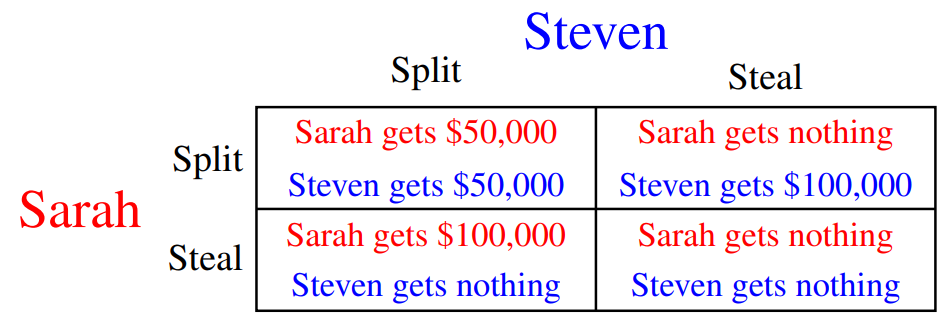
\includegraphics[width=12cm]{images/Split_or_steal.png}
\end{figure}

\section{Nash Equilibrium}
\vocab{Nash Equilibrium} is a set of optimal strategies that work against \textit{all} counter-steategies. This means that if any given player were told the strategies of all their opponents, they still would choose to retain their original strategy. 

\subsection{Matrix games}

\section{Fair Division}
\subsection{Rental harmony problem}
Sperner's lemma

https://www.cs.cmu.edu/~arielpro/15896/docs/paper19b.pdf

%\part{Statistics}
\chapter{Events and Probability}
\section{Introduction}
We will think of performing an experiment which has a set of possible outcomes $\Omega$. We call $\Omega$ the \vocab{sample space}. For example,
\begin{enumerate}[label=(\alph*)]
\item tossing a coin: $\Omega=\{H,T\}$;
\item throwing two dice: $\Omega=\{(i,j)\mid1\le i,j\le 6\}$.
\end{enumerate}

An \vocab{event} is a subset of $\Omega$. An event $A\subseteq\Omega$ occurs if, when the experiment is performed, the outcome $\omega\in\Omega$ satisfies $\omega\in A$. You should think of events as things you can decide have or have not happened by looking at the outcome of your experiment. For example,
\begin{enumerate}[label=(\alph*)]
\item coming up heads: $A=\{H\}$;
\item getting a total of 4: $A=\{(1,3),(2,2),(3,1)\}$.
\end{enumerate}

The \vocab{complement} of $A$ is $A^c\coloneqq \Omega\setminus A$ and means ``$A$ does not occur''. For events $A$ and $B$,

\begin{itemize}
\item $A\cup B$ means ``at least one of $A$ and $B$ occurs'';
\item $A\cap B$ means ``both $A$ and $B$ occur'';
\item $A\setminus B$ means ``$A$ occurs but $B$ does not''.
\end{itemize}

If $A\cap B=\emptyset$ we say that $A$ and $B$ are disjoint -- they cannot both occur.

We will assign a \vocab{probability} $\PP(A)$ to each event $A$. Later on we will discuss general rules (or ``axioms'') governing how these probabilities ought to behave. For now, let’s consider a simple and special case, where $\Omega$ is a finite set, and the probability assigned to a subset $A$ of $\Omega$ is proportional to the size of $A$; that is,
\[ \PP(A)=\frac{|A|}{|\Omega|}. \]

In that case for our examples above, we get:
\begin{enumerate}[label=(\alph*)]
\item for a fair coin, $\PP(A)=\frac{1}{2}$;
\item for the two dice, $\PP(A)=\frac{1}{12}$.
\end{enumerate}

Example (b) demonstrates illustrates the need for counting in the situation where we have a finite number of possible outcomes to our experiment, all equally likely. The sample space $\Omega$ has $36$ elements ($6$ ways of choosing $i$ and $6$ ways of choosing $j$). Since $A=\{(1,3),(2,2),(3,1)\}$ contains $3$ sample points, and all sample points are equally likely, we get $\PP(A)=\frac{3}{36}=\frac{1}{12}$.

We want to be able to tackle much more complicated counting problems.

\section{Counting}
You will have seen before the basic ideas involving permutations and combinations.

\subsection{Arranging distinguishable objects}
Suppose that we have $n$ distinguishable objects (e.g. the numbers $1,2,\dots,n$). How many ways to order them (permutations) are there? If we have three objects $a,b,c$, then the answer is $6$: $abc$, $acb$, $bac$, $bca$, $cab$ and $cba$.

In general, there are $n$ choices for the first object in our ordering. Then, whatever the first object was, we have $n-1$ choices for the second object. Carrying on, we have $n-m+1$ choices for the $m$-th object and, finally, a single choice for the $n$-th. So there are
\[ n(n-1)\cdots2\cdot1=n! \]
different orderings.

\subsection{Arrangements when not all objects are distinguishable}
The number of arrangements of $n$ objects where $\alpha_i$ appears $m_i$ times and $m_1 + \dots + m_k = n$ is
\begin{equation}
\frac{n!}{m_1!m_2!\cdots m_k!}
\end{equation}

If there are just two types of object then, since $m_1 + m_2 = n$, the expression above is just a binomial coefficient
\[ \binom{n}{m_1} = \frac{n!}{m_1!(n-m_1)!} = \binom{n}{m_2} \]
Note: we will always use the notation
\[ \binom{n}{m} = \frac{n!}{m!(n-m)!} \]
Recall the \vocab{binomial theorem}:
\begin{equation}
(x+y)^n = \sum_{m=0}^n \binom{n}{m} x^m y^{n-m}
\end{equation}
You can see where the binomial coefficient comes from because writing
\[ (x+y)^n = (x+y)(x+y)\cdots(x+y) \]
and multiplying out, each term involves one pick from each bracket. The coefficient of $x^my^{n-m}$ is the number of sequences of picks that give $x$ exactly $m$ times and $y$ exactly $n-m$ times and that's the number of ways of choosing the $m$ ``slots'' for the $x$'s.

\begin{exercise}{}{}
How many distinct non-negative integer-valued solutions of the equation
\[ x_1+x_2+\cdots+x_m=n \]
are there?
\end{exercise}
\begin{solution}
Consider a sequence of $n$ $\ast$'s and $m-1$ $|$'s. There is a bijection between such sequences and non-negative integer-valued solutions to the equation. For example, if $m=4$ and $n=3$,
\[ \ast\ast|\quad|\ast| \]
gives the solution $(2,0,1,0)$.

There are $\begin{pmatrix}n+m-1\\n\end{pmatrix}$ sequences of $n$ $\ast$'s and $m-1$ $|$'s and, hence, the same number of solutions to the equation.
\end{solution}

It is often possible to perform quite complex counting arguments by manipulating binomial coefficients. Conversely, sometimes one wants to prove relationships between binomial coefficients and this can most easily be done by a counting argument. One example here is a Vandermonde's Identity: for $k,m,n\ge0$,
\[ \begin{pmatrix}m+n\\k\end{pmatrix}=\sum_{j=0}^k\begin{pmatrix}m\\j\end{pmatrix}\begin{pmatrix}n\\k-j\end{pmatrix} \]
where we use the convention $\begin{pmatrix}m\\j\end{pmatrix}=0$ for $j>m$.

\subsection{An aside on sizes of sets}
In this course, we will often deal with finite collections of objects, as in our counting examples. We will also want to be able to deal with infinite sets, and we will want to distinguish between those that are countable and those that are uncountable.

An infinite set $S$ is called \vocab{countable} (or \vocab{countably infinite}) if there is a bijection between $S$ and the natural numbers $\NN$. That is, we can write $S$ as a list: $S=\{x_1,x_2,x_3,\dots\}=\{x_i\mid i\in\NN\}$. Otherwise $S$ is called \vocab{uncountable}. The natural numbers are themselves countable (take $x_i=i$), as are the rational numbers, but the real numbers, for example, are not.
\pagebreak

\section{The axiomatic approach}
\begin{definition}
A \vocab{probability space} is a triple $(\Omega,\mathcal{F},\PP)$ where
\begin{itemize}
\item $\Omega$ is a set, called the \vocab{sample space};
\item $\mathcal{F}$ is a collection of subsets of $\Omega$, called \vocab{events}, satisfying axioms F1--F3 below.
\item $\PP$ is a \vocab{probability measure}, which is a function $\PP:\mathcal{F}\to\RR$ satisfying axioms P1--P3 below.
\end{itemize}
Axioms of probability:
\begin{itemize}
\item $\mathcal{F}$ is a collection of subsets of $\Omega$, with:
\begin{enumerate}[label=F\arabic*:]
    \item $\Omega\in\mathcal{F}$.
    \item If $A\in\mathcal{F}$, then also $A^c\in\mathcal{F}$.
    \item If $\{A_i,i\in I\}$ is a finite or countably infinite collection of members of $\mathcal{F}$, then $\bigcup_{i\in I}A_i\in\mathcal{F}$.
\end{enumerate}
\item $\PP$ is a function from $\mathcal{F}$ to $\RR$, with:
\begin{enumerate}[label=P\arabic*:]
    \item For all $A\in\mathcal{F}$, $\PP(A)\ge0$.
    \item $\PP(\Omega)=1$.
    \item If $\{A_i,i\in I\}$ is a finite or countably infinite collection of members of $\mathcal{F}$, and $A_i\cap A_j=\emptyset$ for $i\neq j$, then $\PP\brac{\bigcup_{i\in I}A_i}=\sum_{i\in I}\PP(A_i)$.
\end{enumerate}
\end{itemize}
\end{definition}

\chapter{Discrete Random Variables}
A \vocab{discrete random variable} $X$ on a probability space $(\Omega,F,\PP)$ is a function $X : \Omega \to \RR$ such that
\begin{enumerate}[label=(\alph*)]
\item $\{\omega \in \Omega: X(\omega) = x\} \in F$ for each $x \in \RR$
\item $\Im{X} \coloneqq X(\Omega) = \{X(\omega): \omega \in \Omega\}$ is a finite or countable subset of $\RR$.

% https://courses.maths.ox.ac.uk/pluginfile.php/93417/mod_resource/content/8/PrelimsProb_MT23_26Sep2023.pdf
\end{enumerate}

\part{Appendices}
\appendix
\chapter{H3 Mathematics}
\section{A Level past year papers}
\subsection*{2023}
\begin{enumerate}
\item \begin{enumerate}[label=(\alph*)]
\item Prove that, for any real numbers $a_1,a_2,\dots,a_n$,
\[ a_1+a_2+\cdots+a_n\le\sqrt{n}\sqrt{a_1^2+a_2^2+\cdots+a_n^2}. \]
\item Prove that, for any positive real numbers $x$, $y$ and $z$,
\[ \sqrt{\frac{x+y}{x+y+z}}+\sqrt{\frac{y+z}{x+y+z}}+\sqrt{\frac{z+x}{x+y+z}}\le\sqrt{6}. \]
\item Hence solve the equation
\[ 2\sqrt{\frac{x+3}{x+6}}+\sqrt{\frac{6}{x+6}}=\sqrt{6}. \]
\end{enumerate}

\begin{solution} \
\begin{enumerate}[label=(\alph*)]
\item Square both sides, apply Cauchy--Schwarz.
\item Let 
\[ a_1=\sqrt{\frac{x+y}{x+y+z}}, \quad a_2=\sqrt{\frac{y+z}{x+y+z}}, \quad a_3=\sqrt{\frac{z+x}{x+y+z}}, \]
then apply (a) to the above three real numbers.
\item Let $y=3$, $z=3$, then apply (b).

Equality in the Cauchy--Schwarz inequality holds if and only if
\[ \brac{\sqrt{\frac{x+3}{x+6}},\sqrt{\frac{6}{x+6}},\sqrt{\frac{x+3}{x+6}}}=\lambda\brac{1,1,1} \]
for some $\lambda>0$. This happens exactly when $x=3$.
\end{enumerate}

\item 

\item 

\item Let $n$ stones be placed in fixed positions on a line. Each stone is painted using one of four colours (red, white, yellow or blue) in such a way that no two adjacent stones are the same colour. Let $r_n$ be the number of ways of painting the stones such that the first and last stones are both red. Let $s_n$ be the number of ways of painting the stones so that the first stone is red but the last stone is not red.
\begin{enumerate}[label=(\alph*)]
\item Explain why $r_1=1$, $r_2=0$, $s_1=0$ and $s_2=3$.
\item Find a formula for $r_n+s_n$ and explain why $r_{n+1}=s_n$.
\item Using mathematical induction, or otherwise, prove that for all $n\ge4$,
\[ r_n=\frac{3^{n-1}+3(-1)^{n-1}}{4}. \]
\item Now let $n$ stones, where $n>1$, be placed on a circle with numbered positions. Find the number of ways of painting these stones, using at most four distinct colours, in such a way that no two adjacent stones are the same colour.
\end{enumerate}
\end{solution}

\begin{solution} \
\begin{enumerate}[label=(\alph*)]
\item If $n=1$, then the first stone is also the las stone, and there is thus only $1$ way to paint the stone red. So
\[ r_1=1. \]
Since the first stone is red and the last stone, which is the first stone, is red, there is no way to paint the stone such that the last (first) stone is not red. So
\[ s_1=0. \]
If $n=2$, then the first and last (second) stones must be painted red but in doing so they will become adjacent stones painted red, which violates the condition that no two adjacent stones are the same colour. Hence
\[ r_2=0. \]

\item We use the following notation:
\begin{align*}
R&\coloneqq\{\text{painting arrangements such that first and last stones are red}\};\\
S&\coloneqq\{\text{painting arrangements such that first stone is red and last stone is not red}\};\\
T&\coloneqq\{\text{painting arrangements such that first stone is red}\}.
\end{align*}
By definition of $r_n$ and $s_n$,
\[ |R|=r_n, \quad |S|=s_n. \]
Since $R$ and $S$ are mutually exclusive such that $R\cup S=T$, we have
\[ |T|=|R\cup S|=|R|+|S|=r_n+s_n. \]
On the other hand,
\[ T=1\times\underbrace{3\times3\times\cdots\times3}_{n-1}=3^{n-1}. \]
Thus \[ r_n+s_n=3^{n-1}. \]
Observe that if $n+1$ stones are painted in such a way that the first and last stones are both red, then the $n$-th stone must necessarily be non-red since no two adjacent stones can share the sae colour. Therefore, the number of ways to paint $n+1$ stones such that the first and last stones are both red is equal to the number of ways to paint $n$ stones such that the first stone is red and the last stone is not red. Thus, $r_{n+1}=s_n$.

\item 
\item 
\end{enumerate}
\end{solution}

\end{enumerate}

\pagebreak

\subsection*{2022}
\begin{enumerate}
\item 

\item 

\item 

\item \begin{enumerate}[label=(\alph*)]
\item Let $a$ and $b$ be positive numbers such that $a+b=1$. Using a sketch graph of $y=\ln x$, for $x>0$, show that
\[ u^av^b\le au+bv \]
for positive $u$ and $v$.

\item Let $a_1,a_2,a_3,\dots$ be a sequence of positive numbers. Define
\[ G_n=\sqrt[n]{a_1a_2\cdots a_n}\text{ and }A_n=\frac{a_1+a_2+\cdots+a_n}{n}. \]
\begin{enumerate}[label=(\roman*)]
    \item Use the result of part (a) to prove that the sequence $\brac{n(G_n-A_n)}$ is non-increasing.
    \item Let the first 3 terms of the sequence $(a_n)$ be 1, 2 and 4. Define a suitable $a_n$, for $n\ge4$, so that $\brac{n(G_n-A_n)}$ is constant for $n\ge3$.
\end{enumerate}
\end{enumerate}

\begin{solution} \
\begin{enumerate}[label=(\alph*)]
\item Sketch the graph $y=\ln x$ for $x>0$, defined on the closed bounded interval $[u,v]$ for two positive real numbers $u<v$.

Since $a+b=1$, the real number $au+bv$ lies in the interval $[u,v]$; that is,
\[ u\le au+bv\le v. \]

Note that the equation of the straight line joining $(u,\ln u)$ and $(v,\ln v)$ is given by
\[ y-\ln u=\frac{\ln v-\ln u}{v-u}\cdot(x-u). \]

When $x=au+bv$, the $y$-value on this straight line reads off
\[ y=a\ln u+b\ln v. \]

Since $y=\ln x$ is concave, the $y$-value read off the straight line is at most the $y$-value read off the curve $y=\ln x$, and thus it follows that
\[ a\ln u+b\ln v\le\ln(au+bv) \]
or equivalently,
\[ u^ab^v\le a+bv. \]

\item 
\end{enumerate}
\end{solution}

\item 
\item 
\item \begin{enumerate}[label=(\alph*)]
\item The diagram below shows a $3\times3$ array of circles, five of which are shaded. Of the 20 edges linking pairs of adjacent (including diagonally adjacent) circles, 11 link a shaded and an unshaded circle.
\begin{enumerate}[label=(\roman*)]
    \item Describe or draw a $3\times3$ array of circles for which more than 11 edges link a shaded and an unshaded circle and state the number of such edges.
\end{enumerate}
The second diagram shows how the edges for a $4\times4$ array of circles can be grouped into square blocks (consisting of 6 edges) along a diagonal and arrowhead shapes (consisting of 4 edges) elsewhere. For clarity the circles are not shown.
\begin{enumerate}[resume*]
    \item For the edges of an $n\times n$ array of circles grouped as in the second diagram, state the number of square blocks and arrowhead shapes that would be required.
    \item Explain why at most 3 of the edges in an arrowhead shape can link a shaded and an unshaded circle.
\end{enumerate}
\item In the $3\times3$ grid below, some of the squares are shaded. The number in each unshaded square shows the number of shaded squares with which the unshaded square shares a vertex. The sum of all the numbers, 12, is the score of this arrangement of shaded and unshaded squares.
\begin{enumerate}[label=(\roman*)]
    \item Explain, why, for any such arrangement, the score is unaltered by shading each unshaded square and vice versa.
    \item Find the maximum possible score for an $n\times n$ grid and prove that it can be attained.
\end{enumerate}
\end{enumerate}
\end{enumerate}
\pagebreak

\subsection*{2021}
\begin{enumerate}
\item 

\item Let $a$, $b$, $c$ and $r$ be positive real numbers.
\begin{enumerate}[label=(\alph*)]
\item Prove that
\[ a^r(a-b)(a-c)+b^r(b-c)(b-a)+c^r(c-a)(c-b)\ge0. \]
\item Hence, or otherwise, prove that
\begin{enumerate}[label=(\roman*)]
    \item $a^3+b^3+c^3+3abc\ge a^2(b+c)+b^2(c+a)+c^2(a+b)$,
    \item $\displaystyle\frac{1}{a^5}+\frac{1}{b^5}+\frac{1}{c^5}+\frac{a+b+c}{a^2b^2c^2}\ge\frac{b^2+c^2}{a^3b^2c^2}+\frac{c^2+a^2}{a^2b^3c^2}+\frac{a^2+b^2}{a^2b^2c^3}$.
\end{enumerate}
\end{enumerate}

\begin{solution} \
\begin{enumerate}[label=(\alph*)]
\item WLOG assume $a\ge b\ge c$. Then the given expression can be rewritten as
\[ \underbrace{a^r(a-b)(a-c)}_{(1)}+\underbrace{(b-c)[b^r(b-a)-c^r(c-a)]}_{(2)}. \]
For (1), since $a\ge b$ and $a\ge c$, we have $a-b\ge0$ and $a-c\ge0$. Since $a>0$, we then have
\[ a^r(a-b)(a-c)\ge0. \]
Now for (2), since $b\ge c$ we have
\[ b^r(b-a)-c^r(c-a)\ge c^r(b-a-c+a)=c^r(b-c)\ge0. \]
Thus we have proven the given statement.

\item Choose $r=1$, by (a), we have
\[ a(a-b)(a-c)+b(b-c)(b-a)+c(c-a)(c-b)\ge0. \]
Expanding LHS gives us the desired statement.

\item The term $\dfrac{a+b+c}{a^2b^2c^2}$ can be seen as $\dfrac{1}{ab^2c^2}+\dfrac{1}{bc^2a^2}+\dfrac{1}{ca^2b^2}$. This term can be compared to the term $3abc$ in the first part. From this observation, we consider Schur's inequality exhibited by
\[ \frac{1}{a}\brac{\frac{1}{a^2}-\frac{1}{b^2}}\brac{\frac{1}{a^2}-\frac{1}{c^2}}+\frac{1}{b}\brac{\frac{1}{b^2}-\frac{1}{c^2}}\brac{\frac{1}{b^2}-\frac{1}{a^2}}+\frac{1}{c}\brac{\frac{1}{c^2}-\frac{1}{a^2}}\brac{\frac{1}{c^2}-\frac{1}{b^2}}\ge0. \]
Expanding gives us
\begin{align*}
&\frac{1}{a^5}-\frac{1}{a^3c^2}-\frac{1}{a^3b^2}+\frac{1}{ab^2c^2}\\
&+\frac{1}{b^5}-\frac{1}{b^3a^2}-\frac{1}{b^3c^2}+\frac{1}{bc^2a^2}\\
&+\frac{1}{c^5}-\frac{1}{c^3b^2}-\frac{1}{c^3a^2}+\frac{1}{ca^2b^2}\ge0.
\end{align*}
Thus
\begin{align*}
\brac{\frac{1}{a^5}+\frac{1}{b^5}+\frac{1}{c^5}}+\brac{\frac{1}{ab^2c^2}+\frac{1}{bc^2a^2}+\frac{1}{ca^2b^2}}\\
&\ge\brac{\frac{1}{a^3c^2}+\frac{1}{a^3b^2}}+\brac{\frac{1}{b^3a^2}+\frac{1}{b^3c^2}}+\brac{\frac{1}{c^3b^2}+\frac{1}{c^3a^2}}.
\end{align*}
which gives us the desired inequality.
\end{enumerate}
\end{solution}

\item Let $u$ and $v$ be quadratic functions of $x$ and let
\[ y=\frac{u}{v}. \]
\begin{enumerate}[label=(\alph*)]
\item Use mathematical induction to prove that
\[ v\dv[n+2]{y}{x}+(n+2)\dv{v}{x}\dv[n+1]{y}{x}+\binom{n+2}{2}\dv[2]{v}{x}\dv[n]{y}{x}=0, \]
for $n\ge1$.
\item Now assume that $v=(\alpha-x)^2$ for some real number $\alpha$ and, for all positive integers $n$, define
\[ z_n=\frac{(\alpha-x)^{n+2}}{n!}\dv[n]{y}{x}. \]
Use the result of part (a) to prove that $z_1,z_2,z_3,\dots$ is an arithmetic progression. By writing $y$ as partial fractions, or otherwise, show that the common difference is $u(\alpha)$.
\end{enumerate}
\end{enumerate}
\pagebreak

\subsection*{2020}
\begin{enumerate}
\item \begin{enumerate}[label=(\roman*)]
\item For any positive integer $n$ and positive numbers $x$ and $y$, prove that
\[ \brac{(n-1)x+y}^n\ge n^nx^{n-1}y. \]
\item Hence, for any positive numbers $a$, $b$ and $c$ such that $abc=1$, prove that
\[ (1+a)^2(1+b)^3(1+c)^4>256. \]
\end{enumerate}

\begin{solution} \
\begin{enumerate}[label=(\roman*)]
\item Apply AM--GM on $\underbrace{x+\cdots+x}_{n-1}+y$.

\item Watching out for the various powers of 2, 3 and 4, we rewrite
\begin{align*}
&(1+a)^2(1+b)^3(1+c)^4\\
&=\brac{(2-1)1+a}^2\cdot\brac{(3-1)\frac{1}{2}+b}^3\cdot\brac{(4-1)\frac{1}{3}+c}^4\\
&\ge\brac{2^2\cdot1^{2-1}\cdot a}\cdot\brac{3^3\cdot\brac{\frac{1}{2}}^{3-1}\cdot b}\cdot\brac{4^4\cdot\brac{\frac{1}{3}}^{4-1}\cdot c}\\
&=256abc=256
\end{align*}
where equality (for AM--GM) holds if and only if $a=\frac{1}{2}$, $b=\frac{1}{3}$ and $c=\frac{1}{4}$, which is impossible as it contradicts the given condition of $abc=1$. Thus equality never holds, and so the inequality is a strict one.
\end{enumerate}
\end{solution}

\item 

\item For any non-negative integer $n$, the function $P_n$ is defined by
\[ P_n(t)=\sum_{i=0}^n\frac{t^i}{i!}. \]
\begin{enumerate}[label=(\roman*)]
\item Use mathematical induction to prove that
\[ \int_0^tx^ne^{-x}\dd{x}=n!\brac{1-e^{-t}P_n(t)}. \]
\item State the value of 
\[ \int_0^\infty x^ne^{-x}\dd{x}, \]
and briefly justify your answer.
\item For $n>t>0$, prove that
\[ \brac{1+\frac{t}{n}}^n\le P_n(t)<\brac{1-\frac{t}{n}}^{-n}. \]
\end{enumerate}

\begin{solution} \
\begin{enumerate}[label=(\roman*)]
\item Formalise by stating the statement we want to prove:
\[ P(n):\int_0^tx^ne^{-x}\dd{x}=n!\brac{1-e^{-t}P_n(t)}, \quad n=0,1,\dots \]
When $n=0$, we must prove that
\[ \int_0^tx^0e^{-x}\dd{x}=0!\brac{1-e^{-t}P_0(t)}. \]
The working is direct:
\begin{align*}
\int_0^tx^0e^{-x}\dd{x}&=\int_0^te^{-x}\dd{x}\\
&=\sqbrac{-e^{-x}}_0^t\\
&=-e^{-t}+1\\
&=\underbrace{0!}_{=1}(1-e^{-1}\underbrace{P_0(t)}_{=1})
\end{align*}

Assume that $P(n)$ holds, we want to prove that
\[ P(n+1):\int_0^tx^{n+1}e^{-x}\dd{x}=(n+1)!\brac{1-e^{-t}P_{n+1}(t)} \]
holds.

Integrating by parts, let
\[ u=x^{n+1}, \quad \dv{v}{x}=e^{-x}, \]
we have
\begin{align*}
&\int_0^tx^{n+1}e^{-x}\dd{x}\\
&=\sqbrac{-x^{n+1}e^{-x}}_0^t-\int_0^t(n+1)x^n\brac{-e^{-x}}\dd{x}\\
&=\brac{-t^{n+1}e^{-t}}+(n+1)\int_0^tx^ne^{-x}\dd{x}\\
&=(n+1)!\brac{1-e^{-t}\brac{P_n(t)+\frac{t^{n+1}}{(n+1)!}}}\\
&=(n+1)!\brac{1-e^{-t}P_{n+1}(t)}
\end{align*}

\item \[ \int_0^\infty x^ne^{-x}\dd{x}=\lim_{t\to\infty}n!\brac{1-e^{-t}P_n(t)}=n! \]
since $\displaystyle\lim_{t\to\infty}\frac{P_n(t)}{e^t}=0$.

\item We start by proving the LHS:
\[ \brac{1+\frac{t}{n}}^n\le P_n(t). \]
Using binomial expansion,
\[ \brac{1+\frac{t}{n}}^n=\sum_{k=0}^n\binom{n}{k}\frac{t^k}{n^k}. \]
We want to show that 
\[ \sum_{k=0}^n\binom{n}{k}\frac{t^k}{n^k}\le\sum_{k=0}^n\frac{t^k}{k!}. \]
This can be achieved if we are able to prove that
\[ \frac{\binom{n}{k}}{n^k}\le\frac{1}{k!} \]
for $k=0,1,2,\dots,n$. And this is best approached by working backwards: since for all $j=0,1,2,\dots,n$, it holds that
\[ \frac{n-(j-1)}{n}\le1, \]
we must have that
\[ \frac{n\times(n-1)\times\cdots\times(n-(k-1))}{n\times n\times\cdots\times n}\le1. \]
Thus,
\[ \frac{n!}{(n-k)!k!}\frac{1}{n^k}\le\frac{1}{k!} \]
and we have proved that
\[ \frac{\binom{n}{k}}{n^k}\le\frac{1}{k!} \]
for $k=0,1,2,\dots,n$, as planned. This then implies that
\[ \brac{1+\frac{t}{n}}^n=\sum_{k=0}^n\binom{n}{k}\frac{t^k}{n^k}\le\sum_{k=0}^n\frac{t^k}{k!}. \]

\

We now prove the RHS:
\[ P_n(t)<\brac{1-\frac{t}{n}}^{-n}. \]
Note that $n>t>0$, which implies that $-n$ is a negative integer and $\absolute{-\frac{t}{n}}<1$, flagging out the warrant for us to apply Newton's binomial expansion:
\begin{align*}
\brac{1-\frac{t}{n}}^{-n}&=1+(-n)\brac{-\frac{t}{n}}+\frac{(-n)(-n-1)}{2!}\brac{-\frac{t}{n}}^2+\frac{(-n)(-n-1)(-n-2)}{3!}\brac{-\frac{t}{n}}^3+\cdots\\
& +\frac{(-n)(-n-1)(-n-2)\cdots(-n-(k-1))}{k!}\brac{-\frac{t}{n}}^k+\cdots\\
&=1+t+\frac{n(n+1)}{2!}\brac{\frac{t}{n}}^2+\frac{n(n+1)(n+2)}{3!}\brac{\frac{t}{n}}^3+\cdots\\
&+\frac{n(n+1)(n+2)\cdots(n+(k-1))}{k!}\brac{\frac{t}{n}}^k+\cdots\\
&=1+t+\frac{1\brac{1+\frac{1}{n}}}{2!}t^2+\frac{1\brac{1+\frac{1}{n}}\brac{1+\frac{2}{n}}}{3!}t^3+\cdots+\frac{1\brac{1+\frac{1}{n}}\brac{1+\frac{2}{n}}\cdots\brac{1+\frac{k-1}{n}}}{k!}t^k+\cdots\\
&>1+t+\frac{t^2}{2!}+\frac{t^3}{3!}+\cdots+\frac{t^n}{n!}\\
&=P_n(t)
\end{align*}
\end{enumerate}
\end{solution}

\end{enumerate}
\pagebreak

\subsection*{2019}
\begin{enumerate}
\item 

\item 

\item A sequence is defined by
\[ x_1=1\text{ and }x_{i+1}=\brac{\frac{i+a}{i+1}}x_i,\:i\ge1. \]
\begin{enumerate}[label=(\roman*)]
\item Assume that $a\ge0$.
\begin{enumerate}[label=(\alph*)]
    \item Prove that $x_i\ge\frac{1}{i}$, for all positive integers $i$.
    \item Prove that
    \[ \sum_{i=n+1}^{2n}x_i\ge\frac{1}{2}, \]
    for all positive integers $n$.
    \item Hence prove that $\displaystyle\sum_{i=1}^\infty x_i$ is unbounded.
\end{enumerate}
\item Assume that $a<0$.
\begin{enumerate}[label=(\alph*)]
    \item Prove that
    \[ a\sum_{i=m}^nx_i=(n+1)x_{n+1}-mx_m \]
    for all positive integers $m$ and $n$ such that $n>m$.
    \item For any sufficiently large integers $m$ and $n$, prove that $x_mx_n\ge0$.
\end{enumerate}
\end{enumerate}

\begin{solution} \
\begin{enumerate}[label=(\roman*)]
\item \begin{enumerate}[label=(\alph*)]
\item We proceed to prove the statement
\[ P(n):x_n\ge\frac{1}{n}, \quad n=1,2,3,\dots \]
$P(1)$ is true since $x_1=1\ge\frac{1}{1}$.

Assume that $P(k)$ holds for some $k\in\ZZ^+$; that is, 
\[ x_k\ge\frac{1}{k}. \]
We want to prove $P(k+1)$ holds; that is,
\[ x_{k+1}\ge\frac{1}{k+1}. \]
Since $x_{k+1}=\brac{\dfrac{k+a}{k+1}}x_k$, by the inductive hypothesis $P(k)$ we deduce that
\[ x_{k+1}=\brac{\frac{k+a}{k+1}}x_k\ge\brac{\frac{k+a}{k+1}}\cdot\frac{1}{k}=\underbrace{\brac{1+\frac{a}{k}}}_{\ge1}\cdot\frac{1}{k+1}\ge\frac{1}{k+1}. \]
Since $P(1)$ holds and $P(k)\implies P(k+1)$ for all $k\in\ZZ^+$, by mathematical induction, $P(n)$ holds for all $n\in\ZZ^+$.

\item 
\begin{align*}
\sum_{i=n+1}^{2n}x_i&=x_{n+1}+x_{n+2}+\cdots+x_{2n}\\
&\ge\frac{1}{n+1}+\frac{1}{n+2}+\cdots+\frac{1}{2n}\\
&\ge\frac{1}{2n}+\frac{1}{2n}+\cdots+\frac{1}{2n}\\
&=\frac{1}{2n}\times n=\frac{1}{2}
\end{align*}

\item Informally, we see that
\begin{align*}
\sum_{i=1}^\infty&=x_1+x_2+\brac{x_3+x_4}+\brac{x_5+x_6+x_7+x_8}+\cdots\\
&\ge1+\frac{1}{2}+\frac{1}{2}+\frac{1}{2}+\cdots
\end{align*}
which provides compelling evidence that $\sum_{i=1}^\infty x_i$ is unbounded.

We not write this argument in a rigorous manner. To show that $\sum_{i=1}^\infty x_i$ is unbounded, one must show that for any $M>0$, there exists $N\in\ZZ^+$ such that
\[ \sum_{i=1}^Nx_i>M. \]
Indeed, given any $M>0$, there exists $k\in\ZZ^+$ so large that
\[ k>2(M-1) \iff 1+k\cdot\frac{1}{2}>M. \]
Thus it follows that
\begin{align*}
\sum_{i=1}^{2^k}x_i&=x_1+x_2+\brac{x_3+x_4}+\brac{x_5+x_6+x_7+x_8}+\cdots+\brac{x_{2^{k-1}+1}+\cdots+x_{2^k}}\\
&>1+\underbrace{\frac{1}{2}+\frac{1}{2}+\cdots+\frac{1}{2}}_{k\text{ terms}}\\
&=1+k\cdot\frac{1}{2}>M.
\end{align*}
\end{enumerate}

\item \begin{enumerate}[label=(\alph*)]
\item By definition, 
\[ x_{i+1}=\brac{\frac{i+a}{i+1}}x_i, \quad i\ge1. \]
So
\[ (i+1)x_{i+1}=(i_1)x_i \iff (i_1)x_{i+1}-ix_i=ax_i. \]
Thus, if $n>m$ we have
\begin{align*}
\sum_{i=m}^n ax_i
&=\sum_{i=m}^n[(i+1)x_{i+1}-ix_i]\\
&=(m+1)x_{m+1}-mx_m\\
&+(m+2)x_{m+2}-(m+1)x_{m+1}\\
&+\vdots\\
&+(n+1)x_{n+1}-nx_n\\
&=(n+1)x_{n+1}-mx_m
\end{align*}
by the method of difference.

\item For We want to prove that there exists a large enough $N\in\NN$ such that if $m,n\ge N$ then $x_mx_n\ge0$. Notice that in the situation when neither of $x_m$ or $x_n$ is zero these two numbers will have the same sign, i.e. either they are both negative or both positive.

By the recursive definition of $x_i$'s, if $n>m$ then
\[ x_n=\frac{n-1+a}{n}\cdot\frac{n-2+a}{n-1}\cdots\frac{m+a}{m+1}x_m. \]
Since $a<0$ is fixed, there exists a sufficiently large positive integer $N$ such that $N-a>0$. Consequently, if $n>m\ge N$, we have 
\[ x_n=\underbrace{\frac{n-1+a}{n}}_{>0}\cdot\underbrace{\frac{n-2+a}{n-1}}_{>0}\cdots\underbrace{\frac{m+a}{m+1}}_{>0}x_m. \]
Hence $x_n$ and $x_m$ are of the same sign.
\end{enumerate}
\end{enumerate}
\end{solution}

\begin{remark}
The question whether one can make use of (a) to solve (b) remains open.
\end{remark}

\item An $n$-digit number uses no digits other than 1, 2 and 3. It does not have any 2s adjacent to each other, and it does not have any 3s adjacent to each other. Let there be $T_n$ such numbers, with $X_n$ of these having first digit 1 and $Y_n$ having first digit 2.
\begin{enumerate}[label=(\alph*)]
\item Prove that, for any $n\ge2$,
\begin{enumerate}[label=(\roman*)]
    \item $Y_n=X_{n-1}+Y_{n-1}$,
    \item $X_n=X_{n-1}+2Y_{n-1}$,
    \item $X_{n+1}=2X_n+X_{n-1}$.
\end{enumerate}
\item Use mathematical induction to prove that, for $n\ge1$,
\[ X_n\equiv n^2-n+1\pmod 4. \]
\item Find and simplify an expression for $T_n\pmod4$.
\end{enumerate}

\item \begin{enumerate}[label=(\roman*)]
\item Use the substitution $t=\dv{u}{x}$ to find the general solution of the equation
\[ \dv[2]{u}{x}=\dv{u}{x}. \]
\item Show that the differential equation can be transformed into the equation
\[ f(x)\dv[2]{u}{x}-\brac{f^\prime(x)+f(x)g(x)}\dv{u}{x}=0 \]
by the substitution
\[ u=e^{-\int f(x)y\dd{x}}. \]
\item A solution curve of the differential equation
\[ \dv{y}{x}=e^{-2x}y^2+3y \]
passes through the point $\brac{0,-\frac{1}{4}}$. Find the equation of the curve.
\end{enumerate}
\end{enumerate}
\pagebreak

\subsection*{2018}
\begin{enumerate}
\item A triangle has sides of lengths $a$, $b$ and $c$ units. In each of the following cases, prove that there is a triangle having sides of the given lengths.
\begin{enumerate}[label=(\roman*)]
\item $\dfrac{a}{1+a}$, $\dfrac{b}{1+b}$ and $\dfrac{c}{1+c}$ units.
\item $\sqrt{a}$, $\sqrt{b}$ and $\sqrt{c}$ units.
\item $\sqrt{a(b+c-a)}$, $\sqrt{b(c+a-b)}$ and $\sqrt{c(a+b-c)}$ units.
\end{enumerate}

\item 
\item 
\item A clothes shop sells a particular make of T-shirt in four different colours. The shopkeeper has a large number of T-shirts of each colour.
\begin{enumerate}[label=(\roman*)]
\item A customer wishes to buy seven T-shirts.
\begin{enumerate}[label=(\alph*)]
    \item In how many ways can he do this?
    \item In how many ways can he do this if he buys at least one of each colour.
\end{enumerate}
\item The shopkeeper places seven T-shirts in a line.
\begin{enumerate}[label=(\alph*)]
    \item In how many ways can she do this?
    \item In how many ways can she do this if no two T-shirts of the same colour are to be next to each other?
    \item Use the principle of inclusion and exclusion to find the number of ways in which she can do this if she has to use at least one T-shirt of each colour but with no other restrictions.
\end{enumerate}
\end{enumerate}

\item A $p \times q$ chessboard can be tessellated with $a \times b$ tiles.

A unit square $(x,y)$ is shaded if and only if $x \equiv y \pmod a$.
\begin{enumerate}[label=(\roman*)]
\item Explain why the following are necessary conditions for such a tessellation
    \begin{enumerate}[label=(\alph*)]
    \item $ab$ is a factor of $pq$.
    \item $p$ and $q$ can be written in the form $ma+nb$ where $m$ and $n$ are non-negative integers.
    \item The $p \times q$ chessboard has $\dfrac{pq}{a}$ shaded squares.
    \end{enumerate}
\item Let $t$ be the smaller of $r$ and $s$ such that
\begin{align*}
&p \equiv r \pmod a \quad 0 \le r < a \\
&q \equiv s \pmod a \quad 0 \le s < a
\end{align*}
    \begin{enumerate}[label=(\alph*)]
    \item Explain why the number of shaded squares in the $p \times q$ chessboard is $\dfrac{pq-rs}{a}+t$.
    \item Hence prove that for a tessellation, either $a \mid p$ or $a \mid q$.
    \end{enumerate}
\end{enumerate}

\begin{solution} \
\begin{enumerate}[label=(\roman*)]
\item \begin{enumerate}[label=(\alph*)]
    \item A $p \times q$ chessboard has $pq$ squares, a $a \times b$ tile has $ab$ squares.
    
    Suppose $k$ tiles are used to tessellate the board. Then $pq=kab$. Hence $ab\mid pq$.

    \item $p$ and $q$ are the height and base of the $p \times q$ chessboard respectively, $a$ and $b$ are the height and base of each $a \times b$ tile respectively. Each tile can be places horizontally or vertically in the tessellation.
    
    If we tessellate the board at the bottom from left to right with $m$ vertical and $n$ horizontal tiles, there will be $ma+nb$ squares at the bottom row of the board. Each row of the board is made up of $q$ squares. So we get $q=ma+nb$.
    
    Similarly, if we tessellate the board on the left from bottom to top, we will get $p=sa+tb$ (with $s$ horizontal and $t$ vertical tiles).
\end{enumerate}

\item \begin{enumerate}[label=(\alph*)]
    \item 
\end{enumerate}
\end{enumerate}
\end{solution}

\item (Dirichlet's approximation theorem) Let $x$ be any positive real numbers and $n$ be any positive integer. Prove that there are integers $a$ and $b$ with $1 \le b \le n$, such that
\[ \absolute{x-\frac{a}{b}}<\frac{1}{bn}. \]

\begin{solution}
For any real number $y$, we write $y=\floor{y}+\{y\}$, where $\floor{y}$ denotes the integer part of $y$ and $\{y\}$ denotes the fractional part of $y$, $0\le \{y\}<1$.

We divide the interval $[0,1)$ into $n$ smaller intervals of measure $\frac{1}{n}$. Consider $\{x\},\{2x\},\dots,\{nx\}$. Let $I_i$ denote the interval $\sqbrac{\frac{i-1}{n},\frac{i}{n}}$, where $1\le i\le n$.

We now consider two cases:

\textbf{Case 1:} Some $\{kx\}$ falls in $I_1$

Then $kx-\floor{kx}=\{kx\}<\frac{1}{n}$.

Dividing both sides by $k$,
\[ \absolute{x-\frac{\floor{kx}}{k}}<\frac{1}{kn}. \]
By taking $a=\floor{kx}$ and $b=k$, we have the inequality.

\textbf{Case 2:} None of $\{kx\}$ falls in $I_1$

This means all $\{kx\}$ fall into $I_2,I_3,\dots,I_n$. By Pigeonhole Principle, at least two $\{kx\}$ fall in the same $I_i$.

Let $\frac{i-1}{n}\le\{px\}<\frac{i}{n}$ and $\frac{i-1}{n}\le\{qx\}<\frac{i}{n}$. Then
\begin{align*}
\absolute{\{px\}-\{qx\}} &< \frac{1}{n} \\
\absolute{(px-\floor{px})-(qx-\floor{qx})} &< \frac{1}{n} \\
\absolute{(px-qx)-(\floor{px}-\floor{qx})} &< \frac{1}{n} \\
\absolute{(p-q)x-(\floor{px}-\floor{qx})} &< \frac{1}{n}
\end{align*}
Dividing both sides by $p-q$,
\[ \absolute{x-\frac{(\floor{px}-\floor{qx})}{p-q}}<\frac{1}{(p-q)n}. \]
WLOG assume $p>q$. Then $1\le p-q<n$. By taking $a=\floor{px}-\floor{qx}$ and $b=p-q$, we have the inequality.
\end{solution}

\item The differential equation
\begin{equation*}\tag{1}
y\dv{y}{x}=x\brac{\dv{y}{x}}^2+1, \quad \text{for }x>0
\end{equation*}
has a solution curve $S$ such that $\dv[2]{y}{x}$ is non-zero for all points of $S$.
\begin{enumerate}[label=(\roman*)]
\item By substituting $t=\dv{y}{x}$ into equation (1) and differentiating with respect to $x$, show that $S$ has equation $y^2=4x$.
\item Show that a straight line is tangent to the curve $S$ if and only if it is itself a solution of the equation.
\end{enumerate}

\item For any positive real number $x$, $\mathrm{n}(x)$ is defined as the nearest integer to $x$, with halves rounded up.

For example, $\mathrm{n}(3.5)=4$, and $\mathrm{n}(\pi)=3$.

\begin{enumerate}[label=(\alph*)]
\item Show that $\sum_{r=1}^3\mathrm{n}\brac{\frac{11}{7}r}=10$.

The diagram shows the line $y=\frac{7}{11}x+\frac{1}{2}$ and the integer $(x,y)$ such that $1\le x\le 5$, $1\le y\le 3$.

\item Find $\sum_{r=1}^5\mathrm{n}\brac{\frac{7}{11}r}$ and explain the connection between your answer and the points underneath the line $y=\frac{7}{11}x+\frac{1}{2}$.

\item The line $y=\frac{7}{11}x+\frac{1}{2}$ is rotated through $180\degree$ about $(3,2)$. Find the equation of the new line in the form $x=my+c$ and hence comment on the connection between
\[ \sum_{r=1}^3\mathrm{n}\brac{\frac{11}{7}r}=\sum_{r=1}^5\mathrm{n}\brac{\frac{7}{11}r}. \]

\item Let $p$ and $q$ be odd integers greater than $1$ and consider the integer points $(x,y)$ such that $1\le x\le\frac{p-1}{2}$, $1\le y\le\frac{q-1}{2}$. Let $N$ be the number of points which lie in between the lines $y=\frac{q}{p}x+\frac{1}{2}$ and $x=\frac{p}{q}y+\frac{1}{2}$.

Explain why $\displaystyle N+\brac{\frac{p-1}{2}}\brac{\frac{q-1}{2}}\equiv0\pmod2$.
\end{enumerate}
\end{enumerate}
\pagebreak

\subsection*{2017}
\begin{enumerate}
\item 
\item \begin{enumerate}[label=(\roman*)]
\item Let $y$ be a differentiable function of $x$. For any positive integer $n$, prove that
\[ \dv[n]{}{x}\brac{xy}=x\dv[n]{y}{x}+n\dv[n-1]{y}{x}. \]
\item For any non-negative integer $n$, define
\[ y_n=e^{x^2}\dv[n]{}{x}\brac{e^{-x^2}}. \]
\begin{enumerate}[label=(\alph*)]
    \item Find $y_0$, $y_1$ and $y_2$.
    \item Prove that $y_{n+2}+2xy_{n+1}+2(n+1)y_n=0$, for $n\ge0$.
    \item Hence prove that $\dv{}{x}\brac{y_{n+1}}=-2(n+1)y_n$, for $n\ge0$.
\end{enumerate}
\end{enumerate}

\item \begin{enumerate}[label=(\alph*)]
\item Consider integer solutions of the equation
\[ 1591x+3913y=9331. \]
Show that there is no solution with $x$ prime.

\item Let $a$, $b$, $r$ and $s$ be integers such that 
\[ ra+sb=1. \]
    \begin{enumerate}[label=(\roman*)]
    \item Prove that, if $a$ and $b$ are both factors of an integer $n$, then $ab$ is a factor of $n$.
    \item Given that any integers $u$ and $v$, prove by construction that there is an integer $x$ such that both
    \[ x\equiv u\pmod a \quad \text{and} \quad x\equiv v\pmod b. \]
    \end{enumerate}
\end{enumerate}

\begin{solution} \
\begin{enumerate}[label=(\alph*)]
\item First we find $\gcd(1591,3913)$ using the Euclidean Algorithm.
\begin{align*}
3913 &= 2\times1591+731 \\
1591 &= 2\times731+129 \\
731 &= 5\times129+86 \\
129 &= 1\times86+43 \\
86 &= 2\times43+0
\end{align*}
Thus $\gcd(1591,3913)=43$. By Bezout's Lemma, there are integer solutions for $1591x+3913y=43$. Since $43\mid9331$, multiplying both sides by some constant, there are also integer solutions for $1591x+3913y=9331$.

To prove by contradiction, we assume that $x$ is prime, and there exists some integer $y$ such that $1591x+3913y=9331$. Dividing both sides by $43$,
\begin{equation*}\tag{$\star$}
37x+91y=217.
\end{equation*}
Observe that $7\mid91y$ and $7\mid217$, so $7\mid37x$.

Since $\gcd(7,37)=1$ so $7\mid x$. By our assumption, $x$ is a prime so $x=7$.

Substituting $x=7$ into ($\star$), we get $y=-\dfrac{6}{13}$, which contradicts $y$ being an integer.

Hence we conclude that $x$ cannot be a prime.

\item \begin{enumerate}[label=(\roman*)]
    \item If $a$ and $b$ are both factors of $n$, then we have $n=pa$ and $n=qb$ for some integers $p$ and $q$.

    Given $ra+sb=1$, we have
    \begin{align*}
    rna+snb &= n\\
    r(qb)a+s(pa)b &= n \\
    (rq+sp)ab &= n
    \end{align*}
    and hence $ab$ is a factor of $n$.

    \item Prove by construction.

    Given that $ra+sb=1$. Multiplying both sides by $v-u$ gives
    \begin{align*}
    ra(v-u)+sb(v-u)&=v-u\\
    ra(v-u)+u&=sb(u-v)+v
    \end{align*}
    We define $x=ra(v-u)+u=sb(u-v)+v$. Then $x\equiv u\pmod a$ and $x\equiv v\pmod b$.
    \begin{remark}
    The above proof shows the \textit{existence} of solution by a construction.
    \end{remark}
\end{enumerate}
\end{enumerate}
\end{solution}

\item Let $\displaystyle I_n=\int_0^\frac{\pi}{4}\tan^nx\dd{x}$.
\begin{enumerate}[label=(\roman*)]
\item For $n>1$, prove that $\displaystyle I_n+I_{n+2}=\frac{1}{n-1}$.
\item Justify the statement that $\tan x\le\dfrac{4}{\pi}x$ on $\sqbrac{0,\dfrac{\pi}{4}}$.
\item Hence, prove that $I_n$ tends to zero as $n$ tends to infinity.
\item Find the sum of the infinite series
\[ 1-\frac{1}{3}+\frac{1}{5}-\frac{1}{7}+\cdots \]
\end{enumerate}

\begin{solution} \
\begin{enumerate}[label=(\roman*)]
\item \begin{align*}
I_n+I_{n-2}
&=\int_0^\frac{\pi}{4}\brac{\tan^nx+\tan^{n-2}x}\dd{x}\\
&=\int_0^\frac{\pi}{4}\tan^{n-2}x\brac{\tan^2x+1}\dd{x}\\
&=\int_0^\frac{\pi}{4}\tan^{n-2}x\cdot\sec^2x\dd{x}\\
&=\sqbrac{\frac{\tan^{n-1}x}{n-1}}_0^\frac{\pi}{4}=\frac{1}{n-1}.
\end{align*}

\item Sketch the graphs of $y=\tan x$ and $y=\frac{4}{\pi}x$ over the interval $\sqbrac{0,\frac{\pi}{4}}$.

Since $y=\tan x$ is convex over $\sqbrac{0,\frac{\pi}{4}}$, it follows that
\[ \tan x\le\frac{4}{\pi}x \]
for all $x\in\sqbrac{0,\frac{\pi}{4}}$.

\item 

\item 
\end{enumerate}
\end{solution}

\item \begin{enumerate}[label=(\roman*)]
\item Explain why the number of ways to distribute $r$ distinct objects, where $r\ge2$, into 2 distinct boxes such that neither is empty is $2^r-2$.
\item Let $S(r,n)$ denote the number of ways to distribute $r$ objects into $n$ identical boxes such that no box is empty.
\begin{enumerate}[label=(\alph*)]
    \item Explain why, for $r\ge3$,
    \[ S(r,3)=2^{r-2}-1+3S(r-1,3). \]
    \item Prove that, for $r\ge3$,
    \[ S(r,3)=\begin{cases}
    0\pmod6 & \text{if }r\text{ is even,}\\
    1\pmod6 & \text{if }r\text{ is odd.}
    \end{cases} \]
\end{enumerate}
\end{enumerate}

\item 
\item 
\item The Fibonacci sequence is defined recursively by $F_{n+1}=F_n+F_{n-1}$ and $F_1=1,F_2=1$.
\begin{enumerate}[label=(\roman*)]
\item Find the periods of Fibonacci sequences modulo $3$ and $4$.
\item For any positive integer $m$, show that we can find two pairs $(F_j,F_{j+1})$ and $(F_k,F_{k+1})$ which are the same modulo $m$ with $1\le j<k\le m^2+1$.
\item For $m$, $j$ and $k$ as in (ii), explain why the Fibonacci sequence modulo $m$ is periodic
with period dividing $k-j$.
\item For any positive integer $m$, prove that there is a Fibonacci number which is a multiple of $m$.
\end{enumerate}0

\begin{solution} \
\begin{enumerate}[label=(\roman*)]
\item Modulo 3: $1, 1, 2, 0, 2, 2, 1, 0, 1, 1, \dots$ has period $8$.

Modulo 4: $1, 1, 2, 3, 1, 0, 1, 1, \dots$ has period $6$.

\item Modulo $m$, there are $m$ possible values $0,1,2,\dots,m-1$. So there are exactly $m^2$ possible distinct pairs $(a,b)$.

If we consider $m^2+1$ pairs of $(F_i,F_{i+1})$ modulo $m$ where $1\le i\le m^2+1$, we can find two pairs $(F_j,F_{j+1})$ and $(F_k,F_{k+1})$ which are the same modulo $m$, by Pigeonhole Principle.

\item This is the same as showing $F_{j+n} \equiv F_{k+n} \pmod m$ for all non negative integer $n$.

We prove using mathematical induction.

Basis step: $P(0)$ and $P(1)$
\[ F_j \equiv F_k \pmod m \quad F_{j+1} \equiv F_{k+1} \pmod m \]

Inductive step: $P(q-1)\land P(q)\implies P(q+1)$ for all $q\ge 1$

Given $F_{j+q-1} \equiv F_{k+q-1} \pmod m$ and $F_{j+q} \equiv F_{k+q} \pmod m$. Then $F_{j+q-1}+F_{j+q} \equiv F_{k+q-1}+F_{k+q}\pmod m$ so $F_{j+q+1}\equiv F_{k+q+1}\pmod m$.

By mathematical induction, the sequence repeats itself after $k-j$ terms. This implies the period of the sequence divides $k-j$.

\item For any positive $m$, by part (iii), the Fibonacci sequence modulo $m$ is periodic. That is, $(F_1,F_2)$ is congruent to $(F_i,F_{i+1})$ modulo $m$ for some $i>2$:
\[ F_i \equiv F_1 \equiv 1 \pmod m \quad F_{i+1} \equiv F_2 \equiv 1 \pmod m \]
Then $F_{i-1}=F_{i+1}-F_i\equiv1-1\equiv0\pmod m$, which means $m\mid F_{i-1}$.

We have proven that there is a Fibonacci number which is a multiple of $m$.
\end{enumerate}
\end{solution}
\end{enumerate}
\pagebreak

\subsection*{Specimen}
\begin{enumerate}
\item 
\item 
\item (Fermat's Little Theorem)
\begin{enumerate}[label=(\roman*)]
\item Let $p$ be an odd prime and let $a$ be an integer not divisible by $p$.
    \begin{enumerate}[label=(\alph*)]
    \item Let $T$ be the set of remainders for $a,2a,\dots,(p-1)a$, when divided by $p$. Show that $T=\{1,2,\dots,p-1\}$.
    \item Hence prove that $a^{p-1}\equiv1\pmod p$.
    \end{enumerate}
\item Let $x$ and $y$ be two integers such that $x^5+y^5$ is divisible by $5$. Prove that $x^5+y^5$ is divisible by $25$.
\end{enumerate}

\begin{solution} \
\begin{enumerate}[label=(\roman*)]
\item \begin{enumerate}[label=(\alph*)]
    \item Let $S=\{1,2,3,\dots,p-1\}$, the set of all non-zero positive remainders obtained when integers are divided by $p$.
    
    \textbf{Known fact:} $p\nmid k$ for all $k\in S=\{1,2,3,\dots,p-1\}$.

    Given that $T$ is the set of remainders when $a,2a,3a,\dots,(p-1)a$ are divided by $p$.
    
    Clearly, $T\subseteq S\cup\{0\}$.
    
    \textbf{Claim 1:} $0\notin T$.
    \begin{proof}
    Prove by contradiction.

    Suppose $0\in T$. Then $p\mid ka$ for some $k\in S=\{1,2,3,\dots,p-1\}$. Since $p$ is prime and $p\nmid a$, we apply Euclid’s Lemma to conclude that $p\mid k$, which contracts Fact 1.]
    
    Thus $T\subseteq S$.
    \end{proof}
    
    \textbf{Claim 2:} $T=S$ itself.
    \begin{proof}
    Prove by contradiction. 
    
    Suppose, on the contrary, that $T\neq S$.
    
    Then, $T\subset S$ (i.e. $T$ is a proper subset of $S$).
    
    Since the sets are finite sets, $n(T)<n(S)=p-1$. By the Pigeonhole Principle, there are (at least) two distinct $ia$ and $ja$ (from the list of $p-1$ terms: $a,2a,3a,\dots,(p-1)a$ -- the ``pigeons''), where $1\le i\neq j\le p-1$ that share the same remainder when divided $p$. The ``holes'' are the elements in $T$; here we get less holes: $n(T)<p-1$ based on our (wrong) assumption.
    \begin{align*}
    ia &\equiv ja \pmod p \\
    ia-ja &\equiv 0\pmod p \\
    (i-j)a &\equiv 0\pmod p
    \end{align*}
    We can cancel $a$ on both sides due to Euclid's lemma. Hence $i\equiv j\pmod p$.
    
    Since both $i$ and $j$ belong to $S$, having them share the same remainder when divided by $p$ means that they are actually the same. Thus $i=j$. This contradicts our initial choice of distinct $ia$ and $ja$.
    
    Hence $T=S=\{1,2,3,\dots,p-1\}$.
    \end{proof}

    \item Let
    \begin{align*}
    a\cdot1 &\equiv r_1 \pmod p \\
    a\cdot2 &\equiv r_2 \pmod p \\
    a\cdot3 &\equiv r_3 \pmod p \\
    &\vdots \\
    a\cdot(p-1) &\equiv r_{p-1} \pmod p
    \end{align*}
    where $r_1,r_2,r_3,\dots,r_{p-1}$ are distinct elements of $T=S=\{1,2,3,\dots,p-1\}$.

    So multiplying the LHS and RHS respectively of these congruence equations,
    \[ a^{p-1}(p-1)!\equiv r_1r_2r_3\cdots r_{p-1} \pmod p \]
    Since $r_1,r_2,r_3,\dots,r_{p-1}$ is just a rearrangement of $1,2,3,\dots,p-1$,
    \[ a^{p-1}(p-1)!\equiv1\cdot2\cdot3\cdots(p-1)\pmod p \]
    or
    \[ a^{p-1}(p-1)!\equiv(p-1)!\pmod p \]
    But $p\nmid(p-1)!$ so by Euclid's lemma,
    \[ a^{p-1}\equiv1\pmod p \]
    as desired.
    \end{enumerate}

\item Prove by cases

Given $5$ divides $x^5+y^5$.

\textbf{Case 1:} either $x$ or $y$ is divisible by 5

WLOG, assume $5\mid x$. Then $x=5k$ for some integer $k$.

Then $x^5=(5k)^5=5^2(5^3k^5)=25t$ so $25\mid x^5$.

Since we can write $y^5=(x^5+y^5)-x^5$, $5\mid y^5$ so $5\mid y$. We can then similarly show that $25\mid y^5$.

Hence $25\mid x^5+y^5$.

\textbf{Case 2:} both $x$ and $y$ are not divisible by $5$

Since $5$ is a prime, by Fermat's Little Theorem, $x^5\equiv x\pmod 5$ and $y^5\equiv y\pmod 5$, so $x^5+y^5\equiv x+y\pmod 5$.

Since $5\mid x^5+y^5$, we have also $5\mid x+y$, i.e. $x+y=5k$ for some integer $k$. We rewrite $y=5k-x$.

Then by binomial expansion,
\[ y^5=(5k-x)^5=\sum_{i=0}^5\binom{5}{i}(5k)^{5-i}(-x)^i \]
which gives $y^5\equiv(-x)^5\pmod {25}$ as all the other terms are divisible by $25$.

Hence $x^5+y^5\equiv0\pmod {25}$.
\end{enumerate}
\end{solution}

\item 
\item 
\item 
\item The figures below show, respectively, a square board of 4 unit squares with one unit square covered, and a triomino consisting of 3 unit squares.

Irrespective of which unit square is covered, a triomino can cover the remaining 3 unit squares of the square board as shown.

Consider a square board made up of $4^n$ squares, where $n\ge1$, with one of the unit squares covered. An example of such a square, with $n=3$, is shown below.

\begin{enumerate}[label=(\roman*)]
\item Explain how, irrespective of unit square is covered, a triomino can be placed on the board in such a way that each quarter of the board now has one unit square covered.
\item Use mathematical induction to prove that, irrespective of which unit square is initially covered, the remaining squares can be covered by triominoes. State the number of triominoes required.
\end{enumerate}
\end{enumerate}

\begin{prbm}[\acrshort{h3math} 2021]
Let $Q=\{1,2,\dots,p-1\}$ for some prime $p$, and let there be $N$ integers in $Q$ whose cubes are congruent to $1$ modulo $p$.
\begin{enumerate}[label=(\alph*)]
\item Use the pigeonhole principle to prove that for each integer $x\in Q$ there is precisely one integer $y\in Q$ such that $xy\equiv1\pmod p$.
\item Explain why the number of choices of integers $x,y,z\in Q$ such that $xyz\equiv1\pmod p$ is $(p-1)^2$.
\item Use the principle of inclusion and exclusion to prove that the number of choices of three different integers $x,y,z\in Q$ such that $xyz\equiv1\pmod p$ is $(p-1)(p-4)+2N$.
\item Hence prove that $N\equiv(p-1)^2\pmod 3$.
\item Given that $p\equiv1\pmod3$, prove that there is an integer $x\in Q$ such that $x^2+x+1\equiv0\pmod p$.
\end{enumerate}
\end{prbm}

\begin{solution} \
\begin{enumerate}[label=(\alph*)]
\item Note that, by Quotient Remainder Theorem, every integer not divisible by $p$ is congruent to an integer in $Q$ modulo $p$, and no two integers in $Q$ are congruent to each other modulo $p$.

We have two parts to prove: existence and uniqueness of inverse modulo $p$

\textbf{Existence:} prove by contradiction

Suppose there is an $x\in Q$ such that for all $y\in Q$, $xy\not\equiv1\pmod p$.

There are $p-1$ possible $y\in Q$, but there are less than $p-1$ possible $xy\in Q$ (since $xy\equiv1\pmod p$ is excluded).

By Pigeonhole Principle, there are two different $y_1,y_2\in Q$ such that $xy_1\equiv xy_2(\not\equiv1)\pmod p$. Then
\[ p\mid xy_1-xy_2 \implies p\mid x(y_1-y_2) \implies p\mid y_1-y_2 \implies y_1\equiv y_2\pmod p \implies y_1=y_2 \]
which is a contradiction. Hence every $x\in Q$ has a $y\in Q$ such that $xy\equiv1\pmod p$.

\textbf{Uniqueness:} prove by contradiction

Suppose there are two different $y_1,y_2\in Q$ such that $xy_1\equiv xy_2(\equiv1)\pmod p$.

The rest is similar to the above, and thus left as an exercise to the reader.

\item Use combinatorics.

There are $p-1$ ways each to choose $x$ and $y$.

By (a), there is only $1$ way to choose $z\in Q$, the modular inverse of $xy$ mod $p$, such that $(xy)z\equiv1\pmod p$.

Hence there is a total number of $(p-1)^2$ choices of $x,y,z$ such that $xyz\equiv1\pmod p$.

\item Let $U$ contain all $(x,y,z)$ such that $xyz\equiv1\pmod p$, $A$ is a subset of $U$ such that $x\equiv y\pmod p$, $B$ is a subset of $U$ such that $x\equiv z\pmod p$, $C$ is a subset of $U$ such that $y\equiv z\pmod p$.

Note that $A\cap B=A\cap C=B\cap C=A\cap B\cap C$ are all subsets of $U$ such that $x\equiv y\equiv z\pmod p$, i.e. this subset of $U$ contains all $(x,x,x)$ such that $x^3\equiv1\pmod p$.

We have $|U|=(p-1)^2$ from (b), $|A|=|B|=|C|=p-1$, and $|A\cap B\cap C|=N$.

By principle of inclusion and exclusion,
\[ |A\cup B\cup C|=3(p-1)-2N. \]
To find the complement of $A\cup B\cup C$, 
\[ |U-(A\cup B\cup C)|=(p-1)^2-\brac{3(p-1)-2N}=(p-1)(p-4)+2N. \]

\item From (c), the number of choices of three different $x,y,z\in Q$ such that $xyz\equiv1\pmod p$ is $(p-1)(p-4)+2N$.

Since the number of combinations of such $x,y,z$ are symmetrical, this number is divisible by $3$. That is,
\begin{align*}
(p-1)(p-4)+2N &\equiv 0 \pmod 3 \\
(p-1)(p-1)-N &\equiv 0 \pmod 3 \\
(p-1)^2 &\equiv N \pmod 3
\end{align*}

\item From (d), $N\equiv(p-1)^2\equiv0\pmod 3 \implies 3\mid N \implies N\ge3$.

There are at least $3$ different $x$ such that $x^3\equiv1\pmod p$. Choose such an $x\in Q$ such that $x\neq1$.
\[ x^3-1 \equiv 0\pmod p \]
Factorising this gives
\[ (x-1)(x^2+x+1) \equiv 0\pmod p \]
Hence
\[ p\mid(x-1)(x^2+x+1) \]
Since $\nmid x-1$ as $x\in\{1,2,\dots,p-1\}$,
\[ p\mid x^2+x+1 \]
thus $x^2+x+1\equiv0\pmod p$
\end{enumerate}
\end{solution}
\pagebreak

\begin{prbm}[\acrshort{h3math} Specimen]
For any positive integer $n$, if one square is removed from a $2^n\times2^n$ checkerboard, the remaining squares can be completely covered by triominoes (an L-shaped domino consisting of three squares).
\end{prbm}

\begin{solution}
Prove by induction.

\textbf{Base case}: $P(1)$ is clearly true.

\textbf{Inductive step}: $P(k)\implies P(k+1)$ is true for all $k$, i.e. if a $2^k\times2^k$ checkerboard with a square removed can be completely covered by triominoes, then a $2^{k+1}\times2^{k+1}$ checkerboard with a square removed can be completely covered by triominoes.

\begin{enumerate}[label=(\roman*)]
\item Divide the $2^{k+1}\times2^{k+1}$ checkerboard into four $2^k\times2^k$ sub-boards.
\item One of the sub-boards include the removed square.
\item WLOG, assume the top left sub-board has the removed square.
\item By induction hypothesis, this sub-board can be covered by triominoes.
\item For the top right sub-board, we cover it with trominoes with a remaining square at the bottom left corner.
\item For the bottom right sub-board, we cover it with trominoes with a remaining square at the top left corner.
\item For the bottom left sub-board, we cover it with trominoes with a remaining square at the top right corner.
\item The remaining three squares from (v) to (vii) are connected and can be covered by one triomino.
\end{enumerate}
\end{solution}

\begin{remark}
Although it is easy to visualise this by drawing it out, always produce a written proof.
\end{remark}
\pagebreak

\begin{prbm}[\acrshort{h3math} Specimen N03]
Functions $f$ and $g$ are defined for $x\in\RR$ by
\[ f(x)=ax+b, \quad g(x)=cx+d \]
where $a,b,c,d$ are constants with $a=\neq0$. Given that $gf=f^{-1}g$, show that
\begin{itemize}
\item either $g$ is a constant function, i.e. $g(x)$ is constant for all $x\in\RR$,
\item or $f^2$ is the identity function, i.e. $ff(x)=x$ for all $x\in\RR$,
\item or $g^2$ is the identity function.
\end{itemize}
\hfill \textbf{[9]}
\end{prbm}

\begin{solution}
Given that $gf=f^{-1}g$,
\begin{align*}
cf(x)+d&=f^{-1}(cx+d)\\
c(ax+b)+d&=\frac{(cx+d)-b}{a}\\
a^2cx+abc+ad&=cx+d-b
\end{align*}
Comparing coefficients,
\[ \begin{cases}
a^2c=c\\
c(a-1)(a+1)=0\\
abc+ad=d-b
\end{cases} \]
and we have three cases to work with.
\end{solution}
\pagebreak

\section{Selected problems from school papers}
\subsection{Number Theory}
\subsection{Analysis}
\begin{enumerate}
\item (2024 DHS Timed Practice Q1) Prove that for any positive real numbers $x,y,z$ satisfying $xy+yz+zx=x+y+z$,
\begin{enumerate}[label=(\alph*)]
\item $x^2+y^2+z^2\le xy+yz+zx\ge3$, and \hfill [3]
\item $\displaystyle\frac{1}{x^2+y+1}+\frac{1}{y^2+z+1}+\frac{1}{z^2+x+1}\le1$ using the Cauchy--Schwarz inequality. \hfill [4]
\end{enumerate}

\begin{solution} \
\begin{enumerate}[label=(\alph*)]
\item By AM--GM, we have $x^2+y^2\ge2xy$. Similarly, $y^2+z^2\ge2yz$ and $z^2+x^2\ge2zx$. Summing up these three equation gives
\[x^2+y^2+z^2\ge xy+yz+zx.\]
For the second part, from the given condition,
\begin{align*}
(xy+yz+zx)^2&=(x+y+z)^2\\
&=x^2+y^2+z^2+2(xy+yz+zx)\\
&\ge3(xy+yz+zx)\quad\text{from the above part}
\end{align*}
and cancelling on both sides gives us the desired inequality.

\item Considering the denominator,
\[(x+y+z)^2\le(1+y+z^2)(x^2+y+1)\]
by Cauchy--Schwarz inequality. Thus
\[\frac{1}{x^2+y+1}\le\frac{1+y+z^2}{(x+y+z)^2}.\]
Similarly,
\[\frac{1}{y^2+z+1}\le\frac{1+z+x^2}{(x+y+z)^2}\]
and
\[\frac{1}{z^2+x+1}\le\frac{1+x+y^2}{(x+y+z)^2}.\]
Summing up the three equations gives
\[\frac{1}{x^2+y+1}+\frac{1}{y^2+z+1}+\frac{1}{z^2+x+1}\le\frac{3+x+y+z+x^2+y^2+z^2}{(x+y+z)^2}.\]
From part (a), we have $xy+yz+zx=x+y+z\ge3$.
Thus
\begin{align*}
\frac{3+x+y+z+x^2+y^2+z^2}{(x+y+z)^2}
&\le\frac{2(x+y+z)+x^2+y^2+z^2}{(x+y+z)^2}\\
&=\frac{2(xy+yz+zx)+x^2+y^2+z^2}{(x+y+z)^2}=1.
\end{align*}
\end{enumerate}
\end{solution}
\end{enumerate}

\subsection{Counting}
\begin{enumerate}
\item (2019 DHS--EJC Prelim Q6) 
You have an unlimited supply of $1\times1$, $1\times2$ and $2\times2$ tiles. Tiles of the same size are indistinguishable.
\begin{enumerate}[label=(\roman*)]
\item Let $T_n$ is the number of ways of tiling a $1\times n$ path.

State the value of $T_1$ and $T_2$. Write down an appropriate recurrence relation between $T_{n+2}$, $T_{n+1}$ and $T_n$. \hfill [1]
\end{enumerate}

Consider the tilings of a $2\times n$ path. (The $1\times2$ tiles can be rotated in the tilings.)

Let $P_n$ be the number of tilings of

Let $Q_n$ be the number of tilings of

\begin{enumerate}[resume*]
\item Show that $P_{n+1}=P_n+Q_n$ for $n\ge1$. Explain your reasoning clearly. \hfill [2]
\item Show that $Q_{n+1}=2P_{n+1}+2Q_{n+1}$ for $n\ge2$. Explain your reasoning clearly. \hfill [4]
\item Use (ii) and (iii) to show that $P_{n+2}+2P_{n-1}=3P_{n+1}+2P_n$ for $n\ge2$. \hfill [2]
\end{enumerate}

It is given that the solution to the above recurrence relation is
\[ P_n=-\frac{(-1)^n}{7}+\frac{1+2\sqrt{2}}{14}(2+\sqrt{2})^n+\frac{1-2\sqrt{2}}{14}(2-\sqrt{2})^n. \]
\begin{enumerate}[resume*]
\item Find the number of distinct ways of tiling a $2\times n$ path. \hfill [2]
\end{enumerate}

\begin{solution} \
\begin{enumerate}[label=(\roman*)]
\item $T_1=1$, $T_2=2$.

$T_{n+2}=T_{n+1}+T_n$ for $n\ge1$.

\item Consider the ``odd'' tile / last tile in a tiling of $P_{n+1}$. It can only be covered by a $1\times1$ or a $1\times2$ tile.

Consider cases:
\begin{itemize}
\item If it is covered by a $1\times1$ tile, the rest for a tiling of $Q_n$.
\item If it is covered by a $1\times2$ tile, the rest form a tiling of $P_n$.
\end{itemize}
Thus $P_{n+1}=P_n+Q_n$.

\item Consider the last column of 2 tiles in a tiling of $Q_{n+1}$. The following cases are possible:
\begin{itemize}
\item $2\times2$ tile: The rest form a tiling of $Q_{n-1}$.
\item $1\times2$ tile (vertical): The rest form a tiling of $Q_n$.
\item Two $1\times1$ tiles: The rest form a tiling of $Q_n$.
\item Two $1\times2$ tiles (horizontal): The rest form a tiling of $Q_{n-1}$.
\item One $1\times1$ tile and one $1\times2$ tile (horizontal): The rest form a tiling of $P_n$. Note that this case counts twice (depending on which tile covers the top line and which tile covers the bottom line).
\end{itemize}
Thus $Q_{n+1}=2Q_n+2Q_{n-1}+2P_n=2P_{n+1}+2Q_{n-1}$ using the result from (ii).

\item Add $P_{n+1}+2P_{n-1}$ to both sides of (iii):
\[ P_{n+1}+2P_{n-1}+Q_{n+1}=P_{n+1}+2P_{n-1}+2P_{n+1}+2Q_{n-1} \]
and thus
\[ P_{n+2}+2P_{n-1}=3P_{n+1}+2P_n \]
using result from (ii).

\item Number of tilings of $2\times n$ path is $Q_n$. Thus
\begin{align*}
Q_n&=P_{n+1}-P_n\\
&=\frac{2}{7}(-1)^n+\frac{1+2\sqrt{2}}{14}(2+\sqrt{2})^n(2+\sqrt{2}-1)+\frac{1-2\sqrt{2}}{14}(2-\sqrt{2})^n(2-\sqrt{2}-1)\\
&=\frac{2}{7}(-1)^n+\frac{5+3\sqrt{2}}{14}(2+\sqrt{2})^n+\frac{5-3\sqrt{2}}{14}(2-\sqrt{2})^n
\end{align*}
\end{enumerate}
\end{solution}

\item 
\end{enumerate}
\pagebreak

%\printbibliography[type=book,title={Books}]
\printbibliography[title={Bibliography}]

%\textbf{Lecture notes:}
%\begin{itemize}
%\item Lecture notes by the University of Oxford.
%\item Lecture notes by the University of Cambridge. %https://dec41.user.srcf.net/notes/
%\item Lecture notes on MIT OpenCourseWare.
%\end{itemize}

\end{document}